% This is the Reed College LaTeX thesis template. Most of the work
% for the document class was done by Sam Noble (SN), as well as this
% template. Later comments etc. by Ben Salzberg (BTS). Additional
% restructuring and APA support by Jess Youngberg (JY).
% Your comments and suggestions are more than welcome; please email
% them to cus@reed.edu
%
% See http://web.reed.edu/cis/help/latex.html for help. There are a
% great bunch of help pages there, with notes on
% getting started, bibtex, etc. Go there and read it if you're not
% already familiar with LaTeX.
%
% Any line that starts with a percent symbol is a comment.
% They won't show up in the document, and are useful for notes
% to yourself and explaining commands.
% Commenting also removes a line from the document;
% very handy for troubleshooting problems. -BTS

% As far as I know, this follows the requirements laid out in
% the 2002-2003 Senior Handbook. Ask a librarian to check the
% document before binding. -SN

%%
%% Preamble
%%
% \documentclass{<something>} must begin each LaTeX document
\documentclass[11pt,twoside]{reedthesis}
\usepackage[paperheight=237mm,paperwidth=168mm,bottom=20mm, top=20mm, outer=1.5cm, inner=2.4cm]{geometry}
% Packages are extensions to the basic LaTeX functions. Whatever you
% want to typeset, there is probably a package out there for it.
% Chemistry (chemtex), screenplays, you name it.
% Check out CTAN to see: http://www.ctan.org/
%%
\usepackage{graphicx,latexsym}
\usepackage{amsmath}
\usepackage{amssymb,amsthm}
\usepackage{longtable,booktabs,setspace}
\usepackage{chemarr} %% Useful for one reaction arrow, useless if you're not a chem major
\usepackage[hyphens]{url}
% Added by CII
\usepackage{hyperref}
\usepackage{lmodern}
\usepackage{float}
\floatplacement{figure}{H}
% End of CII addition
\usepackage{rotating}

% Next line commented out by CII
%%% \usepackage{natbib}
% Comment out the natbib line above and uncomment the following two lines to use the new
% biblatex-chicago style, for Chicago A. Also make some changes at the end where the
% bibliography is included.
%\usepackage{biblatex-chicago}
%\bibliography{thesis}


% Added by CII (Thanks, Hadley!)
% Use ref for internal links
\renewcommand{\hyperref}[2][???]{\autoref{#1}}
\def\chapterautorefname{Chapter}
\def\sectionautorefname{Section}
\def\subsectionautorefname{Subsection}
% End of CII addition

% Added by CII
\usepackage{caption}
\captionsetup{width=5in}
% End of CII addition

% \usepackage{times} % other fonts are available like times, bookman, charter, palatino

% Syntax highlighting #22

% To pass between YAML and LaTeX the dollar signs are added by CII
\title{Global ecological drivers of transpiration regulation in trees}
\author{Víctor Flo Sierra}
% The month and year that you submit your FINAL draft TO THE LIBRARY (May or December)
\date{Dec 2020}
\degree{DOCTORADO EN ECOLOGIA TERRESTRE}
% \division{}
\advisor{Rafael Poyatos López}
\institution{Autonomous University of Barcelona}
% \degree{DOCTORADO EN ECOLOGIA TERRESTRE}
%If you have two advisors for some reason, you can use the following
% Uncommented out by CII
\altadvisor{Jordi Martínez Vilalta}
% End of CII addition

%%% Remember to use the correct department!
\department{Centre de Recerca Ecològica i Aplicacions Forestals}
% if you're writing a thesis in an interdisciplinary major,
% uncomment the line below and change the text as appropriate.
% check the Senior Handbook if unsure.
%\thedivisionof{The Established Interdisciplinary Committee for}
% if you want the approval page to say "Approved for the Committee",
% uncomment the next line
%\approvedforthe{Committee}

% Added by CII
%%% Copied from knitr
%% maxwidth is the original width if it's less than linewidth
%% otherwise use linewidth (to make sure the graphics do not exceed the margin)
\makeatletter
\def\maxwidth{ %
  \ifdim\Gin@nat@width>\linewidth
    \linewidth
  \else
    \Gin@nat@width
  \fi
}
\makeatother

\renewcommand{\contentsname}{Table of Contents}
% End of CII addition

\setlength{\parskip}{0pt}

% Added by CII

\providecommand{\tightlist}{%
  \setlength{\itemsep}{0pt}\setlength{\parskip}{0pt}}

\Acknowledgements{
\setlength{\parindent}{30pt} Mucha gente es co-responsable de este
trabajo, de haberme empujado y acompañado hasta aquí. Me gustaria
empezar agradeciendo a mis directores de tesis, Rafa y Jordi, sin los
que esta tesis no hubiera sido posible, gracias por la oportunidad de
trabajar con vosotros. He sido muy afortunado de haber contado con dos
mentores excelentes en lo profesional y en lo personal. Rafa, tu
dedicación es envidiable, gracias por todas las buenas ideas, los
comentarios y críticas, las correcciones perfectas, por los viajes a
congresos y por sufrir de mi insomnio y jet-lag. Jordi, ha sido un
privilegio tenerte como tutor, por tu conocimiento transversal y
profundo, por tu capacidad inata e inmediata de entenderlo todo, por
mejorar simpre todas las ideas y textos, y por tu calidad humana.\par
Esta tesis tampoco hubiera sido igual sin haber compartido estos quatro
años con tantos buenos compañeros. Gracias a los compañeros de despacho,
a Anna, Javi, Judit, Carlos, Manu, Aina, Marta, Pere y Pol. Creo que
habeis sido los mejores compañeros posibles y que tuve mucha suerte de
acabar en el -150. Sé que me llevo grandes amistades para toda la vida.
No quiero olvidarme tampoco de muchos otros compañeros como Jordi, Sara,
Kevin, Xavi, Vicenç, Joan, Marina, con los que hemos compartido café,
discusiones y charlas. Gracias también a Luciana por acompañarnos en ese
genial viaje relampago por el desierto americano.\par
Gracias también en especial a los compañeros que estan o han pasado por
el grupo. Maurizio, Tere, Miquel, Lucia, Víctor, Raul, Rosella, Pipo,
Mireia, Lies, David, Jacob, Aude, Antonine, Pablo, Luca y Brenda, sin
duda un grupo envidiable. Gracias por tantos buenos momentos, por la
vertiente académica, pero especialmente por las salidas de grupo, por
las barbacoas, cenas y cervezas. Me gustaria agradecer especialmente a
Víctor Granda, por su excelente trabajo, sin el que hubiera sido
imposible enfrentarnos a la dificil tarea de llevar adelante SAPFLUXNET.
Gracias por enseñarme a querer R, pero sobre todo por las risas y los
enfados jugando a basquet.\par
Durante estos años he tenido la suerte de vivir y conocer a mucha gente
lejos de casa. Muchas personas que me han enseñado otras maneras de ver
el mundo. Me gustaria mencionar especialmente a Martin y a Elena,
gracias por acojerme y hacerme sentir como en casa en Salt Lake City.
Gracias por darnos cobijo cuando nos quedamos en la calle por unos dias,
dejarme vuetro coche, y gracias por un viaje inolmidable a Glacier. No
os lo podré agradecer suficiente. Gracias a Bill Anderegg por acojerme
en su laboratorio donde he tenido la suerte de conocer a gente genial
como Kelly, Nicole, Jaycee. Me gustaria agradecer también a Kathy Steppe
por darme la oportunidad de visitar su laboratorio en Ghent y por sus
buenos consejos. A Roberto por enseñarme a intalar mi primera sonda de
flujo de sabia.\par
Gracias también a los que llevan tiempo compartiendo su camino conmigo o
han caminado alguna etapa, me han marcado y ayudado, a los amigos de
toda la vida y a mis compañeros de andanzas musicales. Gracias Pablo,
Marc, Laura, Oscar, Carles, Jordi, Larry, Cristian, Pol, Kuni, Julio,
Lorenzo, Barbara, Edgar, Jan, Arnau. También a Marta, Rosa, Florian,
Daniel Lola, Magdalena y Esther, por haber creído tanto en mi y haber
sido parte de mi vida durante muchos años.\par
Quiero agradecer también a mi familia. A mis abuelos, a mis tios y
primos, por haber sido una referencia.\par
Gracias sobre todo a quien desde hace quatro años es mi compañera de
viaje. Gracias Mari Angeles por tu sonrisa, tu apoyo incondicional y tu
amor. Esta tesis no hubiera sido sin ti. Gracias por ser brillante, por
que es un placer escucharte y por intentar ``salvar al mundo''. Gracias
por dejarme formar parte de tu familia murciana.\par
Gracias finalmente a mis padres, por dejarme decidir mi camino, por
apoyarme en cada decisión que he tomado. Me habeis hecho libre y feliz.
Mil gracias Ana por haber creido en mi, por ser un ejemplo desde que
eramos pequeños, por ser tan buena y trabajadora. Si alguien es
responsable directo de que me lanzara ha recorrer este camino esa eres
tu. Gracias Clara por ser la alegría de nuestra casa y ser una hermana
maravillosa. Gracias Marc y Jose por formar parte de nuestra vida y por
esas charlas sobre tecnologia y negocios. Para acabar, gracias Arnau, el
último fichaje de la familia. ¡Os quiero!\par
}

\Dedication{
\vspace*{4.5cm}
\begin{flushright}
\hfil \textit{“No one will protect what they don't care about;} \break
\hfil \textit{and no one will care about what they have never experiened”} \break
\hfil \textit{} \break
\hfil \text{David Attenborough}
\end{flushright}
\vspace*{\fill}
}

\Preface{

}

\Abstract{
\setlength{\parindent}{30pt} Understanding how climate affects species'
distribution and performance is a central issue in ecology since its
origins. In last decades, however, the interest in this question has
been reactivated by the current context of climate change. Species Niche
Modelling has been widely used to assess shifts in species distribution
and to test the relationship between species' climatic niche and species
physiological and demographic performance, implicitly assuming that
species occurrence portrays the environmental and biotic species'
suitable conditions. Nevertheless it is still largely undetermined
whether these models can portray population and community responses,
particularly in relation to extreme climatic episodes.\par

In this thesis I aim at exploring the capacity of niche modelling to
predict species decay under extreme climatic conditions, particularly
droughts, addressing some constraints of this approach and proposing
possible solutions. To achieve this goal, I counted with 3 vegetation
decay datasets measured in the Spanish SE after the extreme drought year
2013-2014. Two of these datasets were based on defoliation sampling of
individual plants belonging to more than 40 semiarid shrubland species
(chapters 2, 4 and 5), while the other one was based on regional
compiled data of \emph{Pinus halepensis} L. affectation in plots of
\(1 km^2\) (chapter 3). In second chapter I used different Species
Distribution Model (SDMs) algorithms to estimate species' climatic
suitability before (1950-2000) and during the extreme drought, in order
to test the possible correlation between suitability and decay, and
whether the existence of this relationship depended on the applied SDM
algorithm. I consistently found a positive correlation between remaining
green canopy and species' climatic suitability before the event,
suggesting that populations historically living closer to their species'
tolerance limits are more vulnerable to drought. Contrastingly,
decreased climatic suitability during the drought period did not
correlate with remaining green canopy, likely because of extremely low
climatic suitability values achieved during the exceptional climatic
episode. In order to test whether this extremely low suitability values
could derive as a consequence of only considering climatic averages when
calibrating SDMs, in the third chapter I developed a method to include
inter-annual climatic variability into niche characterization. I then
compared the respective capacities of climatic suitabilities obtained
from averaged-based and from inter-annual variability-based niches to
explain demographic responses to extreme climatic events. I found that
climatic suitability obtained from both niches quantifications
significantly explained species demographic responses. However, climatic
suitability from inter-annual variability-based niches showed higher
explanatory capacity, especially for populations that tend to be more
geographically marginal. In the fourth chapter I tried to overcome the
inability of the SDMs to predict populations decay during extreme
conditions, as observed in the second chapter, by using Euclidean
distances to species' niche in the environmental space. I compared the
capacities of both population distances in the climatic environmental
space and population climatic suitability derived from SDMs to explain
population observed physiological and demographic responses to an
extreme event. Additionally, I tested such relationship in populations
located in three different bedrock sites, corresponding to a gradient of
water availability. I found that SDMs-derived suitability failed to
explain population decay while distances to the niche centroid and limit
significantly explained population die-off, highlighting that population
displaced farther from species' niche during the extreme episode showed
higher vulnerability to drought. The results also suggested a relevant
role of some bedrocks buffering species decay responses to extreme
drought events mainly according to soil water holding capacity. Finally,
in the fifth chapter, I used species niche characterizations in the
environmental space and demographic data to address the impact of
extreme events at community level. Particularly, I estimated the
community climatic disequilibrium before and after a drought episode
along a gradient of water availability in three bedrock types.
Disequilibrium was computed as the difference between observed climate
and community-inferred climate, which was calculated as the mean of
species' climatic optimum weighted by species abundance collected in
field surveys. I found that extreme drought nested within a decadal
trend of increasingly aridity led to a reduction in community climatic
disequilibrium, particularly when combined with low water-retention
bedrocks. In addition, community climatic disequilibrium also varied
before the extreme event across bedrock types, according to soils
water-retention capacity. In conclusion, by developing different
techniques, derived from species distribution, that characterize
climatic accuracy at population and community level, this work reveals
the capacity of species climatic niche to explain demographic responses
under climate change-induced episodes of extreme drought.\par
}

	\usepackage{tikz}
\usepackage{parskip}
\usepackage{colortbl}
\usepackage{xcolor}
\usepackage{threeparttable}
\usepackage{pdflscape}
\usepackage{lettrine}
\usepackage{caption}
\usepackage{titlesec}
\usepackage{multirow}
\usepackage{crop}
\usepackage{pdfpages}
\usepackage{caption}
\usepackage{subcaption}
	\usepackage{booktabs}
\usepackage{longtable}
\usepackage{array}
\usepackage{multirow}
\usepackage{wrapfig}
\usepackage{float}
\usepackage{colortbl}
\usepackage{pdflscape}
\usepackage{tabu}
\usepackage{threeparttable}
\usepackage{threeparttablex}
\usepackage[normalem]{ulem}
\usepackage{makecell}
\usepackage{xcolor}
% End of CII addition
%%
%% End Preamble
%%
%
\begin{document}

% Everything below added by CII
  \maketitle

\frontmatter % this stuff will be roman-numbered
\pagestyle{empty} % this removes page numbers from the frontmatter
  \begin{acknowledgements}
    \setlength{\parindent}{30pt} Mucha gente es co-responsable de este
    trabajo, de haberme empujado y acompañado hasta aquí. Me gustaria
    empezar agradeciendo a mis directores de tesis, Rafa y Jordi, sin los
    que esta tesis no hubiera sido posible, gracias por la oportunidad de
    trabajar con vosotros. He sido muy afortunado de haber contado con dos
    mentores excelentes en lo profesional y en lo personal. Rafa, tu
    dedicación es envidiable, gracias por todas las buenas ideas, los
    comentarios y críticas, las correcciones perfectas, por los viajes a
    congresos y por sufrir de mi insomnio y jet-lag. Jordi, ha sido un
    privilegio tenerte como tutor, por tu conocimiento transversal y
    profundo, por tu capacidad inata e inmediata de entenderlo todo, por
    mejorar simpre todas las ideas y textos, y por tu calidad humana.\par
    Esta tesis tampoco hubiera sido igual sin haber compartido estos quatro
    años con tantos buenos compañeros. Gracias a los compañeros de despacho,
    a Anna, Javi, Judit, Carlos, Manu, Aina, Marta, Pere y Pol. Creo que
    habeis sido los mejores compañeros posibles y que tuve mucha suerte de
    acabar en el -150. Sé que me llevo grandes amistades para toda la vida.
    No quiero olvidarme tampoco de muchos otros compañeros como Jordi, Sara,
    Kevin, Xavi, Vicenç, Joan, Marina, con los que hemos compartido café,
    discusiones y charlas. Gracias también a Luciana por acompañarnos en ese
    genial viaje relampago por el desierto americano.\par
    Gracias también en especial a los compañeros que estan o han pasado por
    el grupo. Maurizio, Tere, Miquel, Lucia, Víctor, Raul, Rosella, Pipo,
    Mireia, Lies, David, Jacob, Aude, Antonine, Pablo, Luca y Brenda, sin
    duda un grupo envidiable. Gracias por tantos buenos momentos, por la
    vertiente académica, pero especialmente por las salidas de grupo, por
    las barbacoas, cenas y cervezas. Me gustaria agradecer especialmente a
    Víctor Granda, por su excelente trabajo, sin el que hubiera sido
    imposible enfrentarnos a la dificil tarea de llevar adelante SAPFLUXNET.
    Gracias por enseñarme a querer R, pero sobre todo por las risas y los
    enfados jugando a basquet.\par
    Durante estos años he tenido la suerte de vivir y conocer a mucha gente
    lejos de casa. Muchas personas que me han enseñado otras maneras de ver
    el mundo. Me gustaria mencionar especialmente a Martin y a Elena,
    gracias por acojerme y hacerme sentir como en casa en Salt Lake City.
    Gracias por darnos cobijo cuando nos quedamos en la calle por unos dias,
    dejarme vuetro coche, y gracias por un viaje inolmidable a Glacier. No
    os lo podré agradecer suficiente. Gracias a Bill Anderegg por acojerme
    en su laboratorio donde he tenido la suerte de conocer a gente genial
    como Kelly, Nicole, Jaycee. Me gustaria agradecer también a Kathy Steppe
    por darme la oportunidad de visitar su laboratorio en Ghent y por sus
    buenos consejos. A Roberto por enseñarme a intalar mi primera sonda de
    flujo de sabia.\par
    Gracias también a los que llevan tiempo compartiendo su camino conmigo o
    han caminado alguna etapa, me han marcado y ayudado, a los amigos de
    toda la vida y a mis compañeros de andanzas musicales. Gracias Pablo,
    Marc, Laura, Oscar, Carles, Jordi, Larry, Cristian, Pol, Kuni, Julio,
    Lorenzo, Barbara, Edgar, Jan, Arnau. También a Marta, Rosa, Florian,
    Daniel Lola, Magdalena y Esther, por haber creído tanto en mi y haber
    sido parte de mi vida durante muchos años.\par
    Quiero agradecer también a mi familia. A mis abuelos, a mis tios y
    primos, por haber sido una referencia.\par
    Gracias sobre todo a quien desde hace quatro años es mi compañera de
    viaje. Gracias Mari Angeles por tu sonrisa, tu apoyo incondicional y tu
    amor. Esta tesis no hubiera sido sin ti. Gracias por ser brillante, por
    que es un placer escucharte y por intentar ``salvar al mundo''. Gracias
    por dejarme formar parte de tu familia murciana.\par
    Gracias finalmente a mis padres, por dejarme decidir mi camino, por
    apoyarme en cada decisión que he tomado. Me habeis hecho libre y feliz.
    Mil gracias Ana por haber creido en mi, por ser un ejemplo desde que
    eramos pequeños, por ser tan buena y trabajadora. Si alguien es
    responsable directo de que me lanzara ha recorrer este camino esa eres
    tu. Gracias Clara por ser la alegría de nuestra casa y ser una hermana
    maravillosa. Gracias Marc y Jose por formar parte de nuestra vida y por
    esas charlas sobre tecnologia y negocios. Para acabar, gracias Arnau, el
    último fichaje de la familia. ¡Os quiero!\par
  \end{acknowledgements}

  \hypersetup{linkcolor=black}
  \setcounter{tocdepth}{2}
  \tableofcontents

  \listoftables

  \listoffigures
  \begin{abstract}
    \setlength{\parindent}{30pt} Understanding how climate affects species'
    distribution and performance is a central issue in ecology since its
    origins. In last decades, however, the interest in this question has
    been reactivated by the current context of climate change. Species Niche
    Modelling has been widely used to assess shifts in species distribution
    and to test the relationship between species' climatic niche and species
    physiological and demographic performance, implicitly assuming that
    species occurrence portrays the environmental and biotic species'
    suitable conditions. Nevertheless it is still largely undetermined
    whether these models can portray population and community responses,
    particularly in relation to extreme climatic episodes.\par
    
    In this thesis I aim at exploring the capacity of niche modelling to
    predict species decay under extreme climatic conditions, particularly
    droughts, addressing some constraints of this approach and proposing
    possible solutions. To achieve this goal, I counted with 3 vegetation
    decay datasets measured in the Spanish SE after the extreme drought year
    2013-2014. Two of these datasets were based on defoliation sampling of
    individual plants belonging to more than 40 semiarid shrubland species
    (chapters 2, 4 and 5), while the other one was based on regional
    compiled data of \emph{Pinus halepensis} L. affectation in plots of
    \(1 km^2\) (chapter 3). In second chapter I used different Species
    Distribution Model (SDMs) algorithms to estimate species' climatic
    suitability before (1950-2000) and during the extreme drought, in order
    to test the possible correlation between suitability and decay, and
    whether the existence of this relationship depended on the applied SDM
    algorithm. I consistently found a positive correlation between remaining
    green canopy and species' climatic suitability before the event,
    suggesting that populations historically living closer to their species'
    tolerance limits are more vulnerable to drought. Contrastingly,
    decreased climatic suitability during the drought period did not
    correlate with remaining green canopy, likely because of extremely low
    climatic suitability values achieved during the exceptional climatic
    episode. In order to test whether this extremely low suitability values
    could derive as a consequence of only considering climatic averages when
    calibrating SDMs, in the third chapter I developed a method to include
    inter-annual climatic variability into niche characterization. I then
    compared the respective capacities of climatic suitabilities obtained
    from averaged-based and from inter-annual variability-based niches to
    explain demographic responses to extreme climatic events. I found that
    climatic suitability obtained from both niches quantifications
    significantly explained species demographic responses. However, climatic
    suitability from inter-annual variability-based niches showed higher
    explanatory capacity, especially for populations that tend to be more
    geographically marginal. In the fourth chapter I tried to overcome the
    inability of the SDMs to predict populations decay during extreme
    conditions, as observed in the second chapter, by using Euclidean
    distances to species' niche in the environmental space. I compared the
    capacities of both population distances in the climatic environmental
    space and population climatic suitability derived from SDMs to explain
    population observed physiological and demographic responses to an
    extreme event. Additionally, I tested such relationship in populations
    located in three different bedrock sites, corresponding to a gradient of
    water availability. I found that SDMs-derived suitability failed to
    explain population decay while distances to the niche centroid and limit
    significantly explained population die-off, highlighting that population
    displaced farther from species' niche during the extreme episode showed
    higher vulnerability to drought. The results also suggested a relevant
    role of some bedrocks buffering species decay responses to extreme
    drought events mainly according to soil water holding capacity. Finally,
    in the fifth chapter, I used species niche characterizations in the
    environmental space and demographic data to address the impact of
    extreme events at community level. Particularly, I estimated the
    community climatic disequilibrium before and after a drought episode
    along a gradient of water availability in three bedrock types.
    Disequilibrium was computed as the difference between observed climate
    and community-inferred climate, which was calculated as the mean of
    species' climatic optimum weighted by species abundance collected in
    field surveys. I found that extreme drought nested within a decadal
    trend of increasingly aridity led to a reduction in community climatic
    disequilibrium, particularly when combined with low water-retention
    bedrocks. In addition, community climatic disequilibrium also varied
    before the extreme event across bedrock types, according to soils
    water-retention capacity. In conclusion, by developing different
    techniques, derived from species distribution, that characterize
    climatic accuracy at population and community level, this work reveals
    the capacity of species climatic niche to explain demographic responses
    under climate change-induced episodes of extreme drought.\par
  \end{abstract}
  \begin{dedication}
    \vspace*{4.5cm}
    \begin{flushright}
    \hfil \textit{“No one will protect what they don't care about;} \break
    \hfil \textit{and no one will care about what they have never experiened”} \break
    \hfil \textit{} \break
    \hfil \text{David Attenborough}
    \end{flushright}
    \vspace*{\fill}
  \end{dedication}
\mainmatter % here the regular arabic numbering starts
\pagestyle{fancyplain} % turns page numbering back on

\captionsetup[figure]{font=small} \setlength{\parindent}{30pt}
\setlength{\parskip}{0.2cm plus4mm minus3mm}

\chapter{Introduction}\label{introduction}

\newpage

\section{Transpiration and earth system
functioning}\label{transpiration-and-earth-system-functioning}

Transpiration is a dynamic process in which water from plants evaporates
and diffuses into the atmosphere. Transpiration occurs as a result of
the need to incorporate carbon dioxide for assimilation in
photosynthesis. This is because the carbon dioxide molecule is larger
than the water molecule, and when it enters the plant tissues, water
escapes through the same pathway. Given that plants require proper
hydration to maintain physiological processes, water loss by
transpiration determines the need to absorb and transport large
quantities of water from the soil (Prasad et al. 2008??). Yet,
transpiration also contributes to regulate leaf temperature, keeping it
within an tolerable range for leaf functioning. Thus, carbon uptake and
transpiration water loss are inexorably linked and have to be
dynamically controlled to avoid desiccation and maintain plant function.
This control occurs on the long-term by changes in plant structure and
anatomy, and in the short-term through the regulation of stomatal
aperture in the leaves (Jones 1998). Stomata are small epidermal valves
with a pore aperture that is usually regulated by plant water status and
hydraulic characteristics (Buckley 2005, Buckley 2019). Stomata close to
protect plants from excessive water loss when atmospheric humidity or
water availability drops, but this closure increases physiological
stress due to reduced carbon gain (Bréda et al. 2006, McDowell 2008 ).
Transpiration, which is therefore determined in just a few micrometres
in the leaves, but is the outcome of the plant integrated hydraulics and
chemical signalling upstream, has crucial implications for biological
processes at the whole-plant level such as growth, competition and
survival. These influences scale up to the population and species level
and determine the water, carbon and energy cycles from the local to the
global level (Bonan et al. 2003), which are essential cycles for the
maintenance of life on Earth. Therefore, due to the relevance of
transpiration patterns on climate and Earth system function it is
crucial to correctly understand and model stomatal regulation and
vegetation water use.\par

Within the global hydrological cycle, vegetation transpiration accounts
for about 45,000 \(km^3\) \(yr^{-1}\) of water flowing from the soil to
the atmosphere (Schlesinger and Jasenchko 2014), which represents around
a 40\% of global terrestrial precipitation (Oki and Kanae, 2006).
Vegetation is thus the major user of the precipitation and directly
affects surface runoff and subsurface recharge. Transpiration accounts
for about 61\% of total terrestrial surface evapotranspiration (which is
the sum of transpiration and the abiotic evaporation from canopy and
soil surfaces). However, this proportion is highly variable within and
among regions (Schlesinger and Jasechko 2014), which is largely
explained by the different vegetation structures (e.g., leaf area index,
Wei et al. 2017) and water use strategies. Total land surface
evapotranspiration and its partition between transpiration and
evaporation drives other biosphere processes, such as vegetation
dynamics or energy balance, that in turn produce feedbacks on
evapotranspiration. For instance, transpiration is determinant of energy
balance impacting in land surface temperature through changes in latent
heat, and mediates land-atmosphere feedbacks via soil moisture depletion
(Miralles et al. 2018). It also promotes clouding formation (Aemisegger
et al. 2014) which alters regional albedo and influences large scale
precipitation regimes (Spracklen et al. 2012).\par

At the same time, climate affects vegetation physiology and how it
regulates transpiration. Different tree species have a specific control
of their stomata in response to environmental changes (Klein et al.,
2014), which means that the distribution of these species and their
physiological traits will have consequences for ecosystem functioning
and, ultimately, for global cycles. Environments with high regional
water availability and resources generally support highly diverse and
productive vegetation, whereas unfavourable environments support
slow-growing vegetation and restrict species richness. Fast-growing
plants tend to have higher transpiration rates (Smith and Sperry 2014),
and therefore accelerate the hydrological cycle. There is a large global
heterogeneity both in space and time in water availability distribution,
which drives heterogeneity in vegetation distribution and feedbacks on
the spatio-temporal variability in transpiration patterns.\par

In addition to the water and energy cycles, transpiration is intimately
linked to the carbon cycle through stomatal gas exchange. The carbon
assimilated by plants in photosynthesis depends mainly on the internal
leaves {[}\text{$CO_2$}{]}, which enters the leaves by diffusion at a
rate controlled by stomatal conductance (Ball et al. 1987 ??). At the
plant level, carbon is used for growth and metabolism but drought-driven
reductions in stomatal conductance limit the amount of carbon fixed by
vegetation (Bréda et al. 2006). Drought stress constrains ecosystem
transpiration and photosynthesis, reducing the potential \text{$CO_2$}
uptake by terrestrial ecosystems (van der Molen et al. 2011).
Transpiration could also be affected by atmospheric {[}\text{$CO_2$}{]},
because as atmospheric {[}\text{$CO_2$}{]} increases, the ratio between
carbon intake and water loss increases so that plants would
theoretically maintain similar photosynthetic rates using less water,
leading to more efficient water use (Keenan et al. 2013 ??). However,
\text{$CO_2$} effects on transpiration seem to be complex and `water
savings' not as clear (Walker et al. 2020). In addition, current
{[}\text{$CO_2$}{]} are approaching saturation levels of the Rubisco
enzyme, at least for the \text{$C_3$} plants, which implies that future
increases in atmospheric {[}\text{$CO_2$}{]} will have progressively
less impact on water use efficiency, and therefore on CO2 transpiration
constrain (Flexas et al. 2015 ??, Sage 2002 ??).\par

Stomatal conductance (\(g_s\)) is therefore a central component of
models characterizing land surface processes, since it is the main
regulator of water, energy, carbon and nutrient fluxes between the
terrestrial biosphere and atmosphere (Knauer et al. 2015, Mencuccini et
al 2019). Thus, \(g_s\) is used in many ecosystem and terrestrial
biosphere models at multiple spatial and temporal scales. For example,
it is included in Land Surface Models to resolve the effects of
vegetation (Matheny et al. 2017) on global climate models (Wang and
Dickinson 2012, Fisher and Koven 2020), or in Dynamic Global Vegetation
Models to predict plant dynamics and vegetation distribution and changes
under future climates (Smith et al. 1992). Most ecosystem and
terrestrial biosphere models are parametrized to separately estimate
transpiration --calculated using diverse formulations of stomatal or
canopy conductance (\(G\)) (Knauer et al. 2015)--, soil evaporation and
evaporation of water intercepted by the canopy or the litter layer. The
mechanisms that regulate stomatal behaviour are still not completely
understood, which is reflected in the different ways these processes are
implemented in models. There are several approaches for modelling
\(g_s\) or \(G\), from semi-empirical (Damour et al. 2010??),
mechanistical (Chuang et al. 2006) or models employing optimality
criteria (Wang et al. 2020). Early models, represented vegetation
\(g_s\) and \(G\) responses with a static set of parameters across plant
functional classes or climates (Manzoni et al. 2011). This
oversimplification of diverse species into functional classes leads
these models to great uncertainties (Poulter et al. 2011). Therefore,
new modelling approaches are moving towards a more versatile
characterization of vegetation which could represent the stomatal
responses to environment emerging from an integration of hydraulic
traits (which are increasingly available at the species level,
Mencuccini et al. 2019, Sanchez-Martinez et al. 2020) at the whole-plant
level. There is an increasing recognition that water transport from
roots to leaves play a key role defining plant water use strategy and
stomatal conductance regulation.\par

\section{Transpiration across scales}\label{transpiration-across-scales}

\subsection{Water transport in plants}\label{water-transport-in-plants}

The water in soil and plants moves under high tensions following the
framework of the cohesion-tension theory (Tyree 1997). Water flow (\(J\)
{[}\(cm^3\) \(s^{-1}\){]}) between any two points of the
soil-plant-atmosphere continuum is given by its difference in \(\Psi\)
(\(\Delta\Psi\)) and the resistance --or its inverse, the hydraulic
conductance (\(K_H\) {[}\(cm^3\) \(s^{-1}\) \(MPa^{-1}\){]})-- that the
system exerts to the flow between these two points. This relationship
can be expressed as \(J = K_H·\Delta\Psi\) which is an expression of
Darcy's law (Scheidegger 1974). Within the plant, water moves along a
gradient of water potential (\(\Psi\); normally negative in plant
tissues) from high \(\Psi\) in the soil (i.e.~less negative) to lower
\(\Psi\) (i.e.~more negative) in the leaves. Similarly, water diffuses
out of the leaf and into the atmosphere following a gradient of water
vapour concentration (\(\Delta\Psi\), the difference in water mole
fraction in the air, which could also be expressed as water potential,
see e.g.~Tyree \& Ewers 1991). Water potential --measured as water
pressure in Pascals (Pa)-- is the energy of water per unit volume
compared to pure water and, along the soil-plant-atmosphere system, is
the sum of hydrostatic potential, osmotic potential and gravitational
potential. Hydrostatic potential is the physical pressure that the
system exerts to the water and is positive inside turgid living cells
but negative inside xylem conduits, a tissue conformed by dead cells and
where water is under tension. The osmotic potential is related to a
difference in solute concentration across a semi-permeable membrane,
where the solution with more solutes has a lower \(\Psi\). The
gravitational potential arises because water ascent from soils to leaves
must overcome gravity, but it is only important for tall trees (Franks
2004).\par

Transport of water in unsaturated soil also follows mass conservation
and Darcy's law. Water enters the roots mainly due to a gradient in
hydrostatic pressure maintained largely by the transpiration stream
(Passioura 1988). As soils dry out, the \(\Psi\) of soils decreases
because the matrix potential, i.e.~the negative hydrostatic potential
produced by the force by which water molecules are hold on surfaces,
becomes more negative as the water layer covering soil particles becomes
thinner. This decrease in soil \(\Psi\) produces a parallel decrease in
plant \(\Psi\) in order to maintain water movement into the plant. Water
absorbed by roots reaches xylem vessels, which by the hydrostatic
pressure gradient generated by water evaporation in the leaves
transported downstream. Water transport in plant tissues is therefore
controlled by the combination of water potentials and plant-specific
hydraulic conductivity (\(k\)), which is a measure of conductance per
unit path length. Xylem \(k\) is in turn dependent on water potential
\(k\)(\(\Psi\)), since cavitation and subsequent embolism formation
occur at low \(\Psi\), when the plant is under drought stress. Xylem
\(k\) declines non-linearly with \(\Psi\) typically following a
sigmoidal shape (vulnerability curve), which is characteristic of each
species due to specific anatomical traits of the xylem (Venturas et al.
2017). Once in the leaves, water from the mesophyll, epidermis and guard
cells evaporate into the stomatal cavity. The difference in \(\Psi\)
between the nearly water saturated stomatal cavity and the atmosphere
represents the steepest potential gradient in all the
soil-plant-atmosphere continuum. It is in the plant-atmosphere
interface, therefore, where the control of water loss is critical to
avoid dangerous tensions in the plant tissues. Stomatal control and its
link with plant hydraulics --but also anatomy, size, density and
location of stomata-- determine plant water status (McCulloh et al.
2019). The mechanistic control of stomata in response to environmental
drivers is still not fully understood, although it appears quite evident
that there are feedback processes (and probably feedforward processes)
between stomatal conductance and leaf water status (Jones 1998, Franks
2004), and hormonal or chemical signalling from the roots to the leaves
(Tardieu et al. 1993 ??).\par

Quantification of transpiration and stomatal control by leaves and
canopies also require a careful consideration of aerodynamic processes
involved in the vapour transfer between the leaves and the atmosphere.
Leaf boundary layer conductance also controls the vapour transport
between the leaf and the surrounding air, as this conductance occurs in
series with \(g_s\). Leaf boundary layer conductance depends on
atmospheric turbulent flux inside the canopy and it is generally much
higher than \(g_s\), especially for trees and forests under
well-ventilated conditions. Under these conditions, canopies are
considered well-coupled to the atmosphere and transpiration is largely
controlled by stomata. However, for large-leaved species under poor
ventilation boundary layer conductance can be similar to stomatal
conductance and this can affect estimations of the degree of stomatal
control based on transpiration measurements. When dealing with whole
plants and canopies, not with individual leaves, the sum of all the
plant stomatal conductances and the boundary layer conductance can be
considered as the whole-plant canopy conductance (Jarvis \& McNaughton
1986, Raupach \& Finnigan 1988).\par

\subsection{Upscaling to the stand and ecosystem
levels}\label{upscaling-to-the-stand-and-ecosystem-levels}

The quantification of water transport in the soil-plant-atmosphere
continuum from a micro-scale perspective (i.e.~at the stomata-level) is
a complex challenge due to the heterogeneity of the transporting medium
and the different temporal scales of the water flux drivers (Katul et al
2007). Therefore, most studies on plant water transport have been
undertaken at the organ (leaves) and the plant levels, observing
emergent macroscopic responses of transpiration to environmental
changes. Upscaling from the leaf to the ecosystem level requires
consideration of processes that occur at the level of individual plants
such as hydraulics. In addition, by using a whole-plant level
perspective, the micro-environmental and physiological gradients within
the canopy are integrated, so we can focus on compositional,
size-related patterns that influence the upscaling to the ecosystem.
However, there is further challenge when trying to upscale both in space
and time, due to the heterogeneity of the distribution of processes and
the non-linearities of whole-plant responses shaped by the link between
physiology and ecosystem functioning (Jarvis 1995). Thus, to scale up to
ecosystem, regional or global level, we should make simplifications to
allow a proper estimation of those processes distributions, either by a
representation of the vegetation by functional types, or a description
by hydraulic or functional traits. Both vegetation classes and traits
are suitable for scaling up, but the latter is a more flexible approach
since they are continuous variables, which overcome the rigidness of
vegetation classes (i.e.~functional type or species), and also allows to
include intra-species environmental gradients and variability, and
diversity within the ecosystem (Anderegg et al. 2018).\par

\section{Transpiration
quantification}\label{transpiration-quantification}

There are several methods to quantify evaporative fluxes from the leaf
to the ecosystem level (Shuttleworth 2008), which differ in their
spatial and temporal domain and in their ability to separately measure
transpiration and evapotranspiration. At the ecosystem level, continuous
sub-daily estimations of evapotranspiration are usually performed using
micrometeorological methods such as Bowen ration energy balance (Bowen
1926) and, mainly, Eddy covariance methods (Brutsaert 1982), which are
based on the measure of turbulence fluxes of latent heat and moisture
(see Wang and Dickinson 2012, Kool et al. 2014, Stoy et al. 2019, for
further details). These methods have been standardized, and currently
there is a global network of measuring stations (FLUXNET) that includes
more than 900 sites worldwide (Pastorello et al. 2020). The FLUXNET
network initiative provides a valuable tool to study global land
hydrological fluxes. However, micrometeorological methods do not allow
to easily and directly separate transpiration from evaporation fluxes,
thus requiring partitioning isotopic methods (Kool et al. 2014) or
complex algorithms to isolate the contribution of transpiration (Nelson
et al. 2020). Since some seminal works such as Sellers (1985), several
attempts have been made to estimate regional transpiration and
evapotranspiration patterns using remote sensing (Miralles et al. 2011,
Miralles et al. 2016). Although remote sensing is the best method for
containing continuous estimates of transpiration at large spatial
scales, these estimations (e.g., GLEAM, Miralles et al. 2011) are
indirect and based on the combination of remotely-sensed variables and
models of vegetation responses and surface energy balance.\par

Since the 1970s, several methods have been developed to independently
measure plant level transpiration, however most of them are impractical
in the field, either because of their low temporal resolution and low
ecological representativeness such as leaf gas exchange methods (Evans
\& Santiago 2014), or because of their limited use on a broad scale due
to their elevated cost such as whole-tree gas exchange chambers (Corelli
\& Magnanini 1993) or lysimeters (Howell 2005). Yet one method that can
be applied continuously, unsupervised, for extended periods and at
relatively low cost, is the measurement of sap flow rate (from now on
Sap Flow Methods, see \textbf{Chapter 2 and 3} for details). Sap flow
methods are thermal-based techniques that were first developed by Huber
(1932), which have diversified into different methodologies since then
(e.g.~Cermak 1973, Swanson and Whitfied 1981, Granier 1985). Sap flow
methods basically apply to woody plants and estimate transpiration by
measuring the water flowing through stems (Schulze et al. 1985). To do
that, semi-invasive probes are installed in the trunk and heat is
applied as a tracer of the sap flux. The quantification of the flux can
be largely characterized using 4 major variants: heat balance, heat
dissipation, heat pulse or heat field deformation methods, which follow
different operation principles, probe configuration, and method specific
flux quantification (see \textbf{Chapter 2}, Vandegehuchte and Steppe
2013). Despite their advantages, all sap flow methods suffer from
potential methodological issues, they assume that the sensors
installation does not alter the sap flow, and they rely on a correct
determination of sapwood cross-sectional area to scale punctual
measurements to the whole-tree level (Vandegehuchte and Steppe 2013, see
\textbf{Chapter 2}). However, most of these issues can be addressed
using specific calibration and applying suitable corrections
(e.g.~Clearwater et al. 1999, Richards et al. 2020). Also, sap flow
methods error have been associated with wood properties but not
consistent patterns have been found (Wullschleger et al. 2011).\par

Despite the potential of sap flow measures, the lack of a global
compilation of sap flow measurements has precluded their use to scale up
plant water use strategies and generalize actual transpiration responses
to environmental drivers, at the regional or global scale. Similarly, a
global sap flow database would allow a much better characterization of
species' water use strategies and the underlying functional traits.
Seminal works of sap flow data synthesis have only been able to focus on
answering partial questions, such as the characterization of
transpiration responses along climatic gradients within a species
(Poyatos et al. 2007), or across a few species, typically addressing
responses to single hydroclimatic factors (Oren et al. 1999), or the
various studies focused on maximum water use (Manzoni et al. 2013).
However, increased data availability and the growing trend of data
sharing for reuse, has paved the way to the creation of a global
collaborative database of sap flow measurements (Poyatos et al. 2016). A
preliminary survey conducted in December 2015 showed that potential
contributors could provide data sets for \textgreater{}160 species and
\textgreater{}120 globally distributed sites (Poyatos et al. 2016).
Thus, in 2016 the design of the first global database of sap flow
measurements (SAPFLUXNET) was initiated, with the intention of
gathering, harmonizing and homogenizing the largest possible number of
sap flow data sets at the whole-plant level together with
hydrometeorological variables at the stand-level, and making them freely
available to the scientific community.\par

\section{Transpiration in a changing
world}\label{transpiration-in-a-changing-world}

Forests are changing rapidly in response to climate change and all
models predict that these changes will accelerate in the future
(Anderegg et al. 2020, McDowell et al. 2020). Importantly an improved
understanding of the regulation of tree water use is key to assess both
species vulnerability and the functional changes expected under new
climate regimes (Choat et al. 2018, Brodribb et al. 2020). The
SAPFLUXNET database will allow us to study, for the first time, the
regulation of whole-plant transpiration to environmental changing
conditions from a global perspective. It will enable the observation of
broad patterns of the water use strategies of woody plants and generate
the knowledge to improve predictions of vegetation responses to future
climate scenarios. A first approach to understand global dynamics of
regulation of transpiration at the whole-plant level can be achieved by
using semi-empirical models of sap flow or canopy conductance (\(G\))
responses to key environmental drivers, including atmospheric vapour
pressure deficit, soil moisture and solar radiation. This approach would
allow us to parameterize the plant's transpiration response, obtaining
species-specific maximum values and sensitivities to hydroclimatic
variables, and thus characterizing the corresponding water use
strategies, their spatial distribution and their physiological and
ecological determinants. In addition, this approach may help to study
which hydrometeorological variables are the main drivers of the
regulation of transpiration globally, as well as its bio-geographical
patterns. In this way, modelling efforts, such as LSMs, could be
optimized and focused on the responses to the environmental variables
with greater predictive power.\par

It is expected that water transport through the soil-plant-atmosphere
and its regulation require of a coordination between stomatal behaviour
and hydraulic traits (Meinzer 2002). This coordination is expected
because vegetation has evolved to be adapted to the conditions of its
typical climate (Sanchez‐Martinez et al. 2020), achieving a balance in
its traits in such a way that they optimize the transport of water and
nutrients while maximizing \text{$CO_2$} uptake and fitness (Manzoni et
al. 2013). This coordination of traits at the organ level would be a
good basis to study the water use strategy that entire plant use to cope
with drought, and would pave the way to trait-based models of vegetation
water use at large spatial scales (Eller et al. 2020, Sperry et al.
2019). Thus, if there was a clear correlation between hydraulic traits
(some of which are relatively easily to measure) and water use
strategies, they could be used for parameterization of \(G\) on a
continuous basis.\par

Therefore, a better understanding of transpiration and its regulation is
key under the Earth's system uncertainty added by global change and the
expected increase in drought conditions (Dai 2013). It is expected that
evaporation and precipitation will be globally intensified but unevenly
distributed, which could trigger large forest mortality events, even in
cold or wet places (Allen et al. 2015). This motivates further work to
improve the predictability of global transpiration estimates and
vegetation drought responses, in order to obtain better predictions of
vegetation dynamics and climate, so as to assist in decision-making for
water resource management, climate change mitigation and forest
management.\par

\section{Research aims and outline}\label{research-aims-and-outline}

In this thesis I address the question of whether we can find global
patterns in daily transpiration regulation at the plant level in
response to hydrometeorological drivers using a global database of sap
flow measurements. The ultimate goal is to characterize the global
variation in plant water use strategies and to relate this variation to
ecosystem eco-hydrological conditions and to species traits, emphasizing
plant water relations and hydraulics (\textbf{Chapter 4 and 5}). Prior
to this synthesis work, I first assessed the suitability of sap flow
methods as reliable estimators of the variation in plant water use
(\textbf{Chapter 2}). And, last, but not least, together with the rest
of the members of the sapfluxnet core team, I worked on the compilation
and harmonization of the datasets in SAPFLUXNET database, which is also
presented as part of this thesis (\textbf{Chapter 3}). The specific
objectives for each research chapter are listed bellow:\par

\textbf{Chapter 2}: To test whether there is systematic variability in
sap flow measurements associated with the sap flow method employed.
Here, (i) I compile all sap flow methodological calibrations obtained
under laboratory or field conditions and perform a meta-analysis to
obtain the mean systematic bias, the proportional bias, the linearity,
and the precision of each method. In addition, I test whether (ii) the
performance of each method is associated to wood anatomy or wood
density.\par

\textbf{Chapter 3}: To introduce SAPFLUXNET and explain how the database
was built from individual data sets contributed by the scientific
community. I (i) explain the data structure design, the data
harmonization and quality control process and the overall workflow, (ii)
summarise the main hydrometeorological drivers and metadata documented
in each dataset, and (iii) discuss the potential applications of the
database, its limitations, and future perspectives.\par

\textbf{Chapter 4}: To test the absolute and relative importance of
vapour pressure deficit, soil moisture and solar radiation as drivers of
tree transpiration at the global scale. I quantify the predictive
capacity of each hydrometeorological driver of plant-level canopy
conductance (\(G\)) using empirical models. I explain the differences in
hydrometeorological coupling of \(G\) (i) across biomes and (ii) their
biogeographical patterns as a function of climate, soil properties and
vegetation structure.\par

\textbf{Chapter 5}: To explore water use strategies across tree species
using a trait-based approach, by parameterizing the response of \(G\) to
vapour pressure deficit and soil water content at the species level and
for major taxonomic groups (Angiosperms vs.~Gymnosperms). I aim to
understand how water use strategies emerge from the covariation between
traits, accounting for the influence of tree size and climate. I also
characterize the relationships between transpiration regulation
parameters and key hydraulic and allocation traits among species,
controlling also for the effect produced by differences in
precipitation.\par

\chapter[Bias and uncertainty in sap flow methods]{A synthesis of bias and uncertainty in sap flow methods}

\setlength{\parindent}{0pt} Victor Flo, Jordi Martinez-Vilalta, Kathy
Steppe, Bernhard Schuldt, Rafael Poyatos \newpage
\setlength{\parindent}{30pt}

\section*{Abstract}

Sap flow measurements with thermometric methods are widely used to
measure transpiration in plants. Different method families exist
depending on how they apply heat and track sapwood temperature (heat
pulse, heat dissipation, heat field deformation or heat balance). These
methods have been calibrated for many species, but a global assessment
of their uncertainty and reliability has not yet been conducted. Here we
perform a meta-analysis of 290 individual calibration experiments
assembled from the literature to assess calibration performance and how
this varies across methods, experimental conditions and wood properties
(density and porosity types). We used different metrics to characterize
mean accuracy (closeness of the measurements to the true, reference
value), proportional bias (resulting from an effect of measured flow on
the magnitude of the error), linearity in the relationship between
measurements and reference values, and precision (reproducibility and
repeatability). We found a large intra- and inter-method variability in
calibration performance, with a low proportion of this variability
explained by species. Calibration performance was best when using stem
segments. We did not find evidence of strong effects of wood density or
porosity type in calibration performance. Dissipation methods showed
lower accuracy and higher proportional bias than the other methods but
they showed relatively high linearity and precision. Pulse methods also
showed significant proportional bias, driven by their overestimation of
low flows. These results suggest that Dissipation methods may be more
appropriate to assess relative sap flow (e.g., treatment effects within
a study) and Pulse methods may be more suitable to quantify absolute
flows. Nevertheless, all sap flow methods showed high precision,
allowing potential correction of the measurements when a study-specific
calibration is performed. Our understanding of how sap flow methods
perform across species would be greatly improved if experimental
conditions and wood properties, including changes in wood moisture, were
better reported.\par

\newpage

\section{Introduction}\label{introduction}

Quantifying transpiration of vegetation is of major importance for
hydrological, ecological, and agricultural sciences, since it represents
60-80\% of the water that returns from the land surface to the
atmosphere (Jasechko et al. (2013); Schlesinger \& Jasechko (2014); Wei
et al. (2017)). The study of transpiration and its environmental
sensitivity is essential to understand vegetation water cycling (D. C.
Frank et al. (2015); Konings, Williams, \& Gentine (2017); Novick et al.
(2016)) and to forecast changes in vegetation functioning and
composition under climate change (C. D. Allen, Breshears, \& McDowell
(2015)). Addressing these questions requires non-destructive
measurements of whole-plant transpiration at multiple timescales (S. D.
Wullschleger, Meinzer, \& Vertessy (1998)). Thermal methods of sap flow
measurement show a number of advantages over other methods such as those
based on isotopes tracing or leaf gas exchange (D. M. Smith (1995)), and
have become the most widely used approach to estimate tree-level
transpiration (Poyatos et al. (2016)) (Fig. A1). When compared against
independent estimates of evapotranspiration components, sap flow methods
have provided reasonable qualitative and quantitative results (Diawara,
Loustau, \& Berbigier (1991), Hogg et al. (1997), Kool et al. (2014),
Schlesinger \& Jasechko (2014), Zhang, Manzoni, Katul, Porporato, \&
Yang (2014), but see K. B. Wilson, Hanson, Mulholland, Baldocchi, \&
Wullschleger (2001), A. C. Oishi, Oren, \& Stoy (2008), T. Shimizu et
al. (2015)). However, sap flow measurements may be subject to various
potential sources of error. Some of these errors are related to scaling
sap flow variability both within trees and from tree to stand level (T.
J. Hatton, Moore, \& Reece (1995); Hernandez-Santana,
Hernandez-Hernandez, Vadeboncoeur, \& Asbjornsen (2015); Mitchell,
Irwin, Flanagan, \& Karron (2009)), while others are related to
intrinsic limitations of the methods or to how these methods are applied
(see Vandegehuchte \& Steppe (2013)). Although these biases have been
studied, they have not yet been quantified globally and there is no
conclusive assessment of how they differ across methods or species
characteristics, including wood properties (Poyatos et al. (2016)).\par

Sap flow methods (Vandegehuchte \& Steppe (2013)) can measure sap flow
rate (SF, g h-1 or equivalent units) or sap flux density (i.e., sap flow
rate per unit sapwood area, SFD, cm3 cm-2 h-1 or equivalent units) in a
plant's conductive tissue and can be classified in four families
depending on how they heat the sapwood and how they measure sapwood
temperatures: (1) the Dissipation family, including thermal dissipation
(TD; Granier \& Une (1985)) and transient thermal dissipation (Do \&
Rocheteau (2002), TTD ({\textbf{???}})) methods, which measure the
dissipation of heat from a heated probe inserted in the sapwood with
reference to a reference, non-heated probe; (2) the Pulse family,
including the compensation heat pulse (CHP; Swanson \& Whitfield
(1981)), heat ratio (HR; S. S. Burgess et al. (2001)), T-max (Y. Cohen,
Fuchs, \& Green (1981)), calibrated average gradient (CAG; Testi \&
Villalobos (2009)), sapflow+ (SF+; Vandegehuchte \& Steppe (2012b),
Vandegehuchte, Steppe, \& Phillips (2012)), single probe heat pulse
(SPHP; ({\textbf{???}})) and dual heat pulse methods (Dual; Pearsall,
Williams, Castorani, Bleby, \& Mcelrone (2014)), which all apply heat in
pulses and track sapwood temperature changes caused by thermal
convection and conduction; (3) the Field family, including the heat
field deformation (HFD; N. Nadezhdina (2018); N. Nadezhdina, Cermák, \&
Nadezhdin (1998)) and its derivatives, which measure the shape changes
of a continuous heat field in the sapwood, using axial and tangential
probes; and (4) the Balance family, represented by stem heat balance
(SHB; ({\textbf{???}}); Sakuratani (1981); ({\textbf{???}})) and trunk
heat balance (THB; Čermák, Kučera, \& Nadezhdina (2004); Čermák1973)
methods, which measure the energy balance across a heated wood section.
This latter family is the only one directly measuring sap flow rate,
while all the others measure sap flux density.\par

Methodological errors in sap flux density measurements may be caused by
wounding following probe insertion into the sapwood (except for the
miniaturized non-invasive ones; see (Michael J. Clearwater, Luo, Mazzeo,
\& Dichio (2009); Hanssens, De Swaef, Nadezhdina, \& Steppe (2013);
Schreel \& Steppe (2018)), biological variation in wood parameters and
diverse raw data processing approaches (A. C. Oishi, Hawthorne, \& Oren
(2016); Peters et al. (2018); Vergeynst, Vandegehuchte, McGuire, Teskey,
\& Steppe (2014)). Wounding affects heat and water transport and thus
may disrupt sap flow measurements (Barrett, Hatton, Ash, \& Ball (1995);
S. S. Burgess et al. (2001); S. Green, Clothier, \& Perie (2009); Steve
Green, Clothier, \& Jardine (2003); S. R. Green \& Clothier (1988);
Steppe, Vandegehuchte, Tognetti, \& Mencuccini (2015)), especially
during long-term installations (S. Marañón-Jiménez et al. (2018); A
Wiedemann, Jiménez, Rebman, Cuntz, \& Herbst (2013)). While wound
corrections have been available for a long time for some Pulse family
methods (Steve Green et al. (2003); Swanson \& Whitfield (1981)), they
have only become recently available for other methods such as TD
(Andreas Wiedemann et al. (2016)). Sap flux density methods are also
affected by changes in radial patterns, which are not constant over
time, so these methods have to measure the entire sapwood depth by
sufficiently large probes, or by individual measurement points at
different depths (T. Hatton (1990)). Although some methods have a more
solid theoretical background based on the physics of thermal transport
(Pulse and Balance methods), all of them rely on a certain degree of
empiricism, which may introduce errors caused by biological variability
and/or variation in signal processing approaches: species-specific
empirical calibrations in Dissipation methods (S. Fuchs, Leuschner,
Link, Coners, \& Schuldt (2017)), zero-flow determination or baselining
(Ping Lu, Urban, \& Zhao (2004); Peters et al. (2018)), and different
parameterization of thermal sapwood properties in Pulse and Field
methods (Chen, Miller, Rubin, \& Baldocchi (2012)). These thermal
sapwood parameters could change over time, introducing further errors in
the measurements (e.g.~changes in stem water content; Vergeynst et al.
(2014)). Within the Balance family, those using external heating do not
suffer from potential errors due to wounding, but they all require
zero-flow determination (D. Smith \& Allen (1996)). Balance methods have
often been considered to better integrate spatial variability in sap
flow (Čermák et al. (2004)), but whether they perform generally better
than sap flux density methods remains unknown.\par

Other errors in sap flow measurement may result from not accounting
properly for method-specific assumptions. For many sap flow methods,
natural temperature gradients (NTG) need to be minimized and/or
accounted for to obtain unbiased estimates of sap flow (Reyes-Acosta,
Vandegehuchte, Steppe, \& Lubczynski (2012); Vandegehuchte, Burgess,
Downey, \& Steppe (2015)). Incorrect sensor geometry (misalignment)
affects the accuracy of the measurements (S. S. Burgess et al. (2001);
Cabibel \& F (1991); Ren et al. (2017); Swanson (1983); Swanson \&
Whitfield (1981)). Other application errors, such as those arising from
the incomplete contact of TD probes with the sapwood (Michael J
Clearwater, Meinzer, Andrade, Goldstein, \& Holbrook (1999)) are
difficult to prevent, though they can be reasonably corrected a
posteriori (e.g.~Clearwater correction, K. R. Hultine et al. (2010);
Paudel, Kanety, \& Cohen (2013)). Despite that these application errors
have been well described in individual studies, a general quantification
of these errors for the most employed sap flow methods is currently
lacking.\par

Comparisons of sap flow measurements with respect to a reference method
(hereafter, for simplicity, `sap flow calibrations') are usually aimed
at obtaining species-specific calibrations (Vandegehuchte \& Steppe
(2013)) to assess different parameterizations of wood thermal properties
(Vandegehuchte \& Steppe (2012a)) or to validate empirical corrections
(e.g., wounding, NTG, changes in water content, misalignment; S. S.
Burgess et al. (2001); Vergeynst et al. (2014)). Although few studies
calibrate multiple sap flow methods for different species (S. Fuchs et
al. (2017)), collectively these calibration studies have shown the
inherent limitations of different sap flow methods to deal with low
(Steve Green et al. (2003)) or high flows (S. Green et al. (2009)).
Variability and quality in calibration performance may also be related
to specific wood properties such as wood density (Suleiman, Larfeldt,
Leckner, \& Gustavssor (1999); Wullschleger, Childs, King, \& Hanson
(2011)), especially given the fact that wood density enters the
calculation of sap flux density for some methods (Vandegehuchte \&
Steppe (2012a)) and co-varies with wood moisture content (Looker,
Martin, Jencso, \& Hu (2016)). Because thermal properties of wood are
dependent on both, i.e.~wood density and moisture content (MacLean
(1941)), they might additionally be influenced by wood anatomical traits
such as wood porosity type, i.e.~coniferous, diffuse-porous or
ring-porous wood. In conifers, however, no clear effects of wood density
on calibration variability have been reported (Peters et al. (2018)).
Therefore, a quantitative synthesis of sap flow calibrations, accounting
for variation caused by different flow ranges and wood properties is
needed to generalize and understand the patterns observed in individual
calibration studies.\par

Here, we compile a global database of published sap flow calibrations to
quantify the measurement errors associated with different sap flow
methods and to assess the factors underlying variability across methods.
In assessing calibrations, we distinguished between mean systematic bias
(accuracy), a measure of the average degree of closeness of the
measurements to the value obtained with a reference method; proportional
bias, which occurs when the magnitude of the error is a function of the
flow; linearity in the relationship between measurements and values
obtained with a reference method; and precision, a measure of
reproducibility and repeatability. Our main objective is to assess the
differences in accuracy, proportional bias, linearity and precision
among methodological families and individual sap flow methods; in
addition, we will determine whether calibration performance across
methods is associated with species wood traits (wood density and
porosity type).\par

\section{Material and methods}\label{material-and-methods}

\subsection{Sap flow calibration
datasets}\label{sap-flow-calibration-datasets}

We retrieved sap flow calibration studies of the seven most common
methods (CHP, T-max, HR, HFD, SHB, TD, TTD) applied on trees, palms or
lianas, using standard database searching tools (i.e.~Scopus, Web of
Science and Google Scholar). The search was conducted in June 2017
applying the following keywords: sap fl*, sap flux density, calibration,
potomet*, gravimet*, thermal dissipation, heat pulse, heat balance, heat
field deformation, compensation heat pulse, T-max, and their
combinations. Other sources of data were obtained from the references of
previously collected studies. For each calibration experiment, we
obtained paired observations of sap flow, measured with a thermal method
and with an independent reference method (typically gravimetric or
volumetric). Data was digitized from published figures (using GetData
Graph Digitalizer version 2.26.0.20). We asked the authors to supply the
raw data when these were unavailable from the original publication. We
obtained data from 60 studies (see Table A1) reporting 374 individual
calibration experiments performed on 81 different shrub and trees
species (10,186 data points in total). In the analysis, we only used
calibrations that were properly applied according to our definition
below (i.e.~290 calibrations out of 374) to restrict the variability to
the intrinsic characteristics of the methods.\par

We always considered sap flow observations obtained with the original
parameters of the methods (e.g.~Granier's original calibration for TD),
without applying the coefficients derived from the calibrations
themselves. Some calibrations with TD gave measured K values (i.e.~sap
flow index, calculated from raw sapwood temperature differences) instead
of measured SFD and, in these cases, K values were transformed to SFD
using Granier's original equation and calibration coefficients (Eq. 1, a
= 42.84 \(cm^3 cm^{-2} h^{-1}\), b = 1.231) (Granier \& Une (1985)).
\begin{equation}
SFD = a\times K^b
\end{equation}
For each calibration, we recorded the type of calibration material:
whole plants, whole plants without roots or cut stem segments. We also
assessed whether the sap flow method was properly applied using the best
available protocol specified for each method. We considered a proper
application of Dissipation methods when the probe was shorter than the
sapwood depth and radial profile correction was applied, when the probe
was approximately equal to the sapwood depth, or when the probe was
longer than the sapwood depth and this effect was corrected for
following Clearwater et al. (1999). To test whether our results could
have been affected by this correction, we performed a preliminary
analysis with the same structure as the main statistical model
(cf.~section 1.3.3) comparing TD calibrations with or without the
Clearwater correction and we did not find significant effects on any of
the metrics of calibration performance (cf.~section 1.3.2) (data not
shown). We considered a proper application of Pulse methods when wound
correction was applied and either the probe had multiple measuring
points along the sapwood or a radial sap flow profile correction was
applied. We always considered Balance methods and Field methods as
properly applied, because they always integrate (or account for) spatial
variability of sap flow.\par

Finally, to analyze the influence of wood traits on calibration
performance we used wood density, defined as fresh volume over oven-dry
mass, and wood porosity type of the species employed in each study. Wood
density was supplied in only a few studies (7 species \textasciitilde{}
80 calibration experiments \textasciitilde{} 4 studies). Assuming that
for wood density between-species variability is typically larger than
within-species variability (Siefert et al., 2015; Vilà-Cabrera et al.,
2015), we retrieved wood density of each species from the TRY database
(Kattge et al., 2011). Wood densities of Carica papaya, Phoenix
dactylifera and Vitis vinifera were obtained from Kempe (2014), Fathi
(2014) and Castelan-Estrada (2002), respectively, as they were not
recorded in TRY. When wood density could not be found for a given
species, we used the phylogenetically nearest species of the same genus
if available in TRY (10 of 81 species; e.g.~Citrus sinensis for Citrus
reticulata). We could not estimate wood density for three taxa (Humulus
lupulus, Musa sp. and Siagrus romanzoffiana). A correlation between
calibration-specific and species-level wood density extracted from the
TRY database (r = 0.78, P \textless{} 0.01, n = 12 calibrations, 6
species) indicates that species-level wood density values indeed are
applicable for our purpose, but the results should be interpreted with
caution. Finally, wood porosity was obtained from the InsideWood
database (Wheeler (2011), ({\textbf{???}})), using four categories:
ring-porous, diffuse-porous (i.e.~diffuse and semi-diffuse porous),
conifer and monocots.\par

\subsection{Calibration assessment}\label{calibration-assessment}

Although the reference methods always provide an estimate of sap flow
through plants or stem segments, sap flow measurements can be reported
as SF or SFD. It was not possible for us to interconvert between SF and
SFD in all cases because sapwood areas were not always reported. This
precluded a joint analysis of all the paired observations in the same
linear model because units differ between SF and SFD. To overcome this
problem and to maximize the amount of data considered in the analyses,
we first evaluated calibration performance using four complementary
dimensionless metrics at the calibration level, which allowed us to
analyze globally all calibrations regardless of the magnitude they
reported (SF or SFD). In a second stage, we quantified the variability
in the absolute errors in sap flow measurements across methods and flow
ranges separately for SF and SFD methods. We did not expect differences
between calibrations reported with SF or SFD because the
inter-conversion between them only involves a scalar transformation. In
addition, preliminary analyses confirmed that there was no significant
difference between SF and SFD for any of the calibration performance
metrics reported in this study (Table A2).\par

For the global analysis, the following metrics were calculated for each
calibration (SF and SFD): the average ln ratio (Ln-Ratio) between
measured and reference values as a measure of overall accuracy; the
slope of the relationship between measured and reference sap flow to
characterize proportional bias (Slope); the slope of the ln-ln
relationship between measured and reference sap flow as a measure of
linearity (Slope (ln-ln)); and Z Pearson's Correlation to describe
precision (Z-Cor) (Fig. 1.1). To calculate these metrics, we filtered
out data points with measured or reference flows less or equal to 0. All
calibration metrics and subsequent statistical models were performed in
R 3.4.2 (R Core Team (2017)). For model-based metrics, we always checked
residuals to ensure they satisfied normality and homoscedasticity
assumptions. Accuracy was evaluated as the mean of the natural logarithm
of the ratio between paired measurements (j) of each calibration (i):
\begin{equation}
Ln-Ratio_i = \frac{\sum_{j=1}^{n} ln(\frac{measured_j}{reference_j})_i}{n_i}
\end{equation}
where \(measured_j\) and \(reference_j\) are the paired measurements of
sensor-estimated and reference flow, respectively, and n the number of
paired measurements for each calibration i (see Fig. 1.1). The Ln-Ratio
varies between \(-\infty\) and \(+\infty\), and equals 0 for a
calibration with perfect mean accuracy (i.e.~lack of systematic bias).
We also expressed this metric as the exponential of Ln-ratio minus one
multiplied by 100, as an indicator of accuracy deviation (in \%).\par

The slope of the linear relationship (Eq. 3) describes how the magnitude
of the error changes (linearly) as a function of the reference flow. The
slope of the ln-ln relationship (Eq. 4) captures the linearity between
the measured and the reference flow. Both slope estimates were
calculated for each calibration using a simple linear regression (lm -
package stats):
\begin{equation}
measured_{ij} \sim \beta_{0i}+\beta_{1i}\;reference_{ij}+e_{ij}
\end{equation}
\begin{equation}
ln(measured_{ij}) \sim \beta^{\prime}_{0i}+\beta^{\prime}_{1i}\;ln(reference_{ij}) +e_{ij}
\end{equation}
where \(\beta_{0i}\) and \(\beta'_{0i}\) are the intercepts and
\(\beta_{1i}\) and \(\beta'_{1i}\) are the slopes for each calibration
(\(i\)), and \(j\) indicates individual calibration points. Hereafter,
we will refer to \(\beta_{1i}\) as \(Slope\) and to \(\beta'_{1i}\) as
\(Slope (ln-ln)\); slope values equal to 1 characterize measurements
without proportional bias (Eq. 3) and with high linearity (Eq. 4),
respectively.\par

We used Pearson's correlation coefficients r between measured and
reference flow of each calibration experiment (\(i\)) as a metric to
describe the precision of the methods. The distribution of the resulting
variable was skewed due to the large amount of correlation coefficients
close to 1, so we used Fisher's Z transformation (Eq. 5) to achieve
normality:
\begin{equation}
Z-Cor_i = \frac{1}{2}ln(\frac{1+r_i}{1-r_i})
\end{equation}
Low values of \(Z-Cor\) correspond to low r correlations, and high
values of \(Z-Cor\) correspond to high \(r\) correlations and thus high
precision (data set range \(r\) = {[}0.0491 -- 0.9999{]}; \(r\)= 0.0491
\textasciitilde{} \(z\) = 0.0491; \(r\) = 0.9999 \textasciitilde{} \(z\)
= 5.1594).\par
\begin{figure}[hbt!]

{\centering 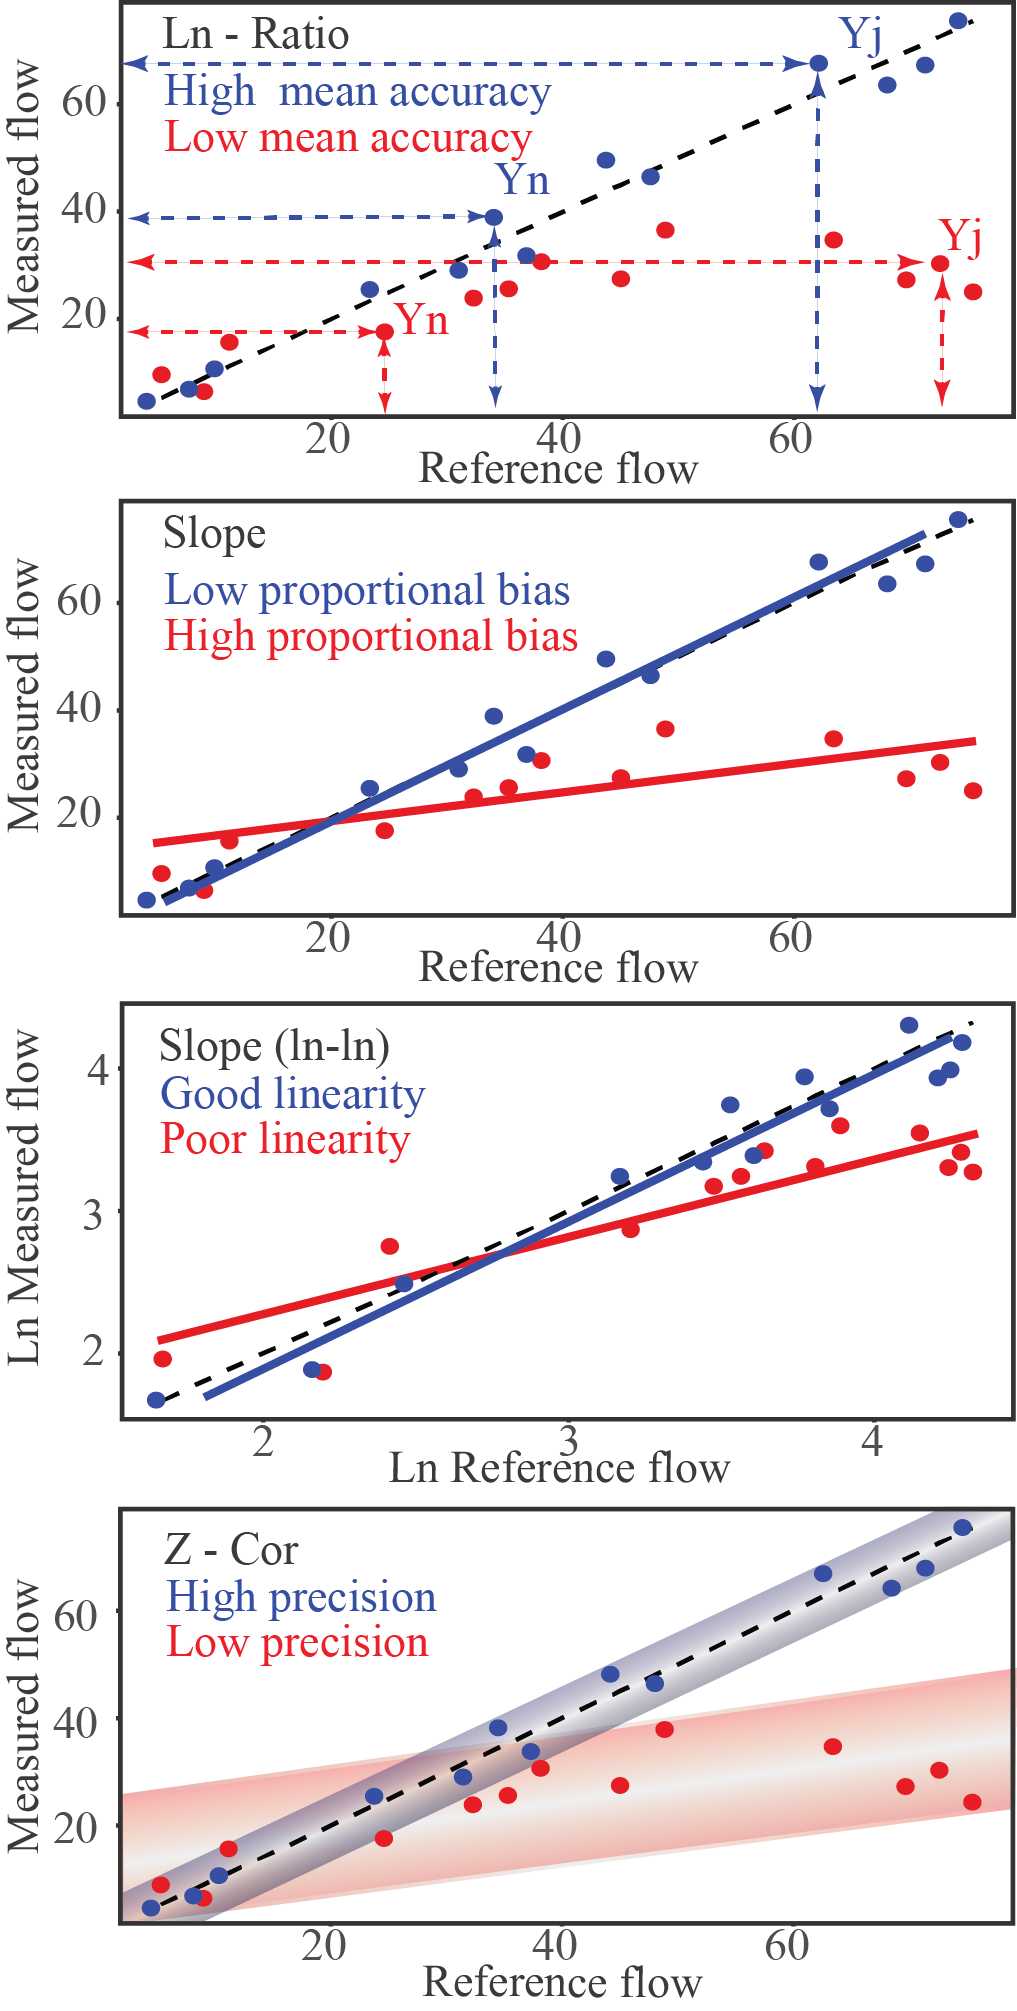
\includegraphics[width=0.55\linewidth]{figure/CH2/PLOTMETRICS} 

}

\caption[Graphical representation of the calibration performance metrics.]{Graphical representation of the calibration performance metrics used in the analyses. Each panel presents the same simulated calibration points, representing plausible data. Blue dots represent an accurate, unbiased, linear and precise calibration, while red dots represent an inaccurate, biased, non-linear and imprecise calibration.}\label{fig:ch2fig1}
\end{figure}
In the analysis of the absolute errors of sap flow measurements, we
calculated the Normalized Root Mean Square Error (NRMSE) for each
calibration (\(i\)) (Eq. 6), separately for SFD and SF methods, in order
to obtain the percentage of absolute error at the mean range of each
calibration (\(i\)).
\begin{equation}
NRMSE_i = \frac{(\sqrt \frac{\sum_{j=1}^{n} (measured_j-reference_j)^2}{n})_i\times 100}{range\;mean_i}
\end{equation}
Subsequently, from the NRMSE and the mean range of each calibration, we
fitted a linear model for each method allowing to quantify the absolute
error (RMSE) at a given sap flow and also to obtain a RMSE at a
reference flow (cf.~section 2.3).\par

\subsection{Statistical analyses}\label{statistical-analyses}

All the analyses were performed using linear mixed-effects models (LMM)
with the package lmer (Bates, Mächler, Bolker, \& Walker (2015)).
Least-square means were estimated with package lsmeans (Lenth (2016))
and used to summarise the effects of fixed factors and to test contrasts
among predictions. In all models, we used the variables Study and
Species as partially crossed random effects (Schielzeth \& Nakagawa
(2013)), as we are interested in taking into account the variability
associated with study and species, and also to analyze within- and
between-group variability. We used Study as we expect experimental
variability between researchers or laboratories, and Species because
calibration performance has been reported to vary across species (S.
Fuchs et al. (2017); D. Smith \& Allen (1996); Steppe et al. (2015)).
For each model, \(R^2_m\) and \(R^2_c\) (marginal and conditional
coefficients of determination, respectively) based on Nakagawa \&
Schielzeth (2013) were calculated using the function r.squaredGLMM of
the package MuMIn (Barton (2017)) in R. Intraclass Correlation
Coefficients (ICC) were also calculated for the random factors to
quantify the proportion of variance within and among groups (low ICC
implies high intra-group variability).\par

In a first analysis, we were interested in assessing the differences in
calibration metrics (Ln-Ratio, Slope, Slope (ln-ln), Z-Cor) between
different families of methods (Family: Pulse, Dissipation, Balance and
Field methods), because methods within a family share similar physical
principles. We also analyzed differences between individual methods with
a sufficient sample size (Method: CHP, T-max, HR, HFD, SHB, TD, TTD). As
the calibration material determines, to a large extent, the experimental
conditions, we also included this variable in our models (Material:
whole plants, whole plants without roots or cut stem segments). For the
analysis of absolute errors of sap flow measurements, we modelled NRMSE
as a function of Method and the Mean Range of SFD (or SF for Balance
methods) in each calibration, as well as their interaction. We used the
same random structure as in previous models.\par 

Finally, we assessed how each calibration metric depended on Wood
Density and Wood Porosity. A first model included all methods available,
with Method interacting with Wood Density as predictors. In order to
test Wood Porosity effects, we fitted separate models for CHP and TD
calibrations, as these two methods were the only ones that had enough
data (\textgreater{} 5 calibrations) for more than one type of porosity.
Separate models were needed because not all wood porosity types were
represented for all methods. In both models we also included Material as
an explanatory cofactor, and the same random structure as in the first
analysis explained above.\par

\section{Results}\label{results}

Most of the published calibrations were performed with Pulse and
Dissipation methods (Table 1.1). In particular, 61\% of the total number
of the properly applied calibrations were conducted using TD or CHP,
followed by HFD and HR. SHB, T-max and TTD methods were less
represented, with 8 -- 14 calibrations each. The metrics extracted from
the raw calibrations were highly variable within methods (Fig. 1.2).
Calibration metrics often followed a quasi-normal distribution, but in
most cases distributions were truncated or skewed, particularly for
methods with fewer calibrations (Fig. 1.2).\par
\begin{table}

\caption[Analysis summary for the different methods and families.]{\label{tab:Ch1T1}Analysis summary for the different methods and families of methods obtained from the LMM models (least-squares means). We provide the four dimensionless metrics: the Ln-ratio as a measure of accuracy, the accuracy deviation calculated as the exponential of the Ln-ratio minus one multiplied by 100, the Slope to characterize the proportional bias, the slope of the ln-ln-relationship, Slope (ln-ln), as a measure of linearity, and Z Pearson’s correlation (Z-Cor) to describe overall precision; n: number of calibrations; studies: number of studies of each method; species: number of different species; r is the correlation calculated as the tanh of Z-Cor.}
\resizebox{\linewidth}{!}{
\fontsize{6}{8}\selectfont
\begin{tabular}[t]{llllll>{\raggedright\arraybackslash}p{2cm}llll}
\toprule
Method & Family & n & studies & species & Ln-Ratio & Accuracy deviation \% & Slope & Slope (ln-ln) & Z-Cor & r\\
\midrule
CHP & Pulse & 63 & 16 & 21 & 0.133 & 14.225 & 0.887 & 0.783 & 1.837 & 0.950\\
T-max & Pulse & 11 & 5 & 6 & -0.053 & -5.162 & 0.614 & 0.697 & 1.755 & 0.942\\
HR & Pulse & 23 & 6 & 7 & -0.145 & -13.498 & 0.845 & 0.841 & 2.000 & 0.964\\
HFD & Field & 57 & 3 & 4 & -0.073 & -7.040 & 0.901 & 0.782 & 2.378 & 0.983\\
SHB & Balance & 8 & 5 & 6 & -0.242 & -21.494 & 0.847 & 0.967 & 2.287 & 0.980\\
TD & Dissipation & 115 & 18 & 35 & -0.519 & -40.488 & 0.683 & 1.066 & 1.711 & 0.937\\
TTD & Dissipation & 14 & 2 & 6 & -0.493 & -38.921 & 0.669 & 0.985 & 1.464 & 0.899\\
all & Pulse & 97 & NA & 30 & 0.012 & 1.167 & 0.844 & 0.787 & 1.874 & 0.954\\
all & Field & 57 & NA & 4 & -0.008 & -0.820 & 0.896 & 0.762 & 2.322 & 0.981\\
all & Balance & 8 & NA & 6 & -0.244 & -21.650 & 0.854 & 0.972 & 2.294 & 0.980\\
all & Dissipation & 129 & NA & 37 & -0.464 & -37.153 & 0.681 & 1.052 & 1.666 & 0.931\\
\bottomrule
\end{tabular}}
\end{table}
\begin{figure}[hbt!]

{\centering 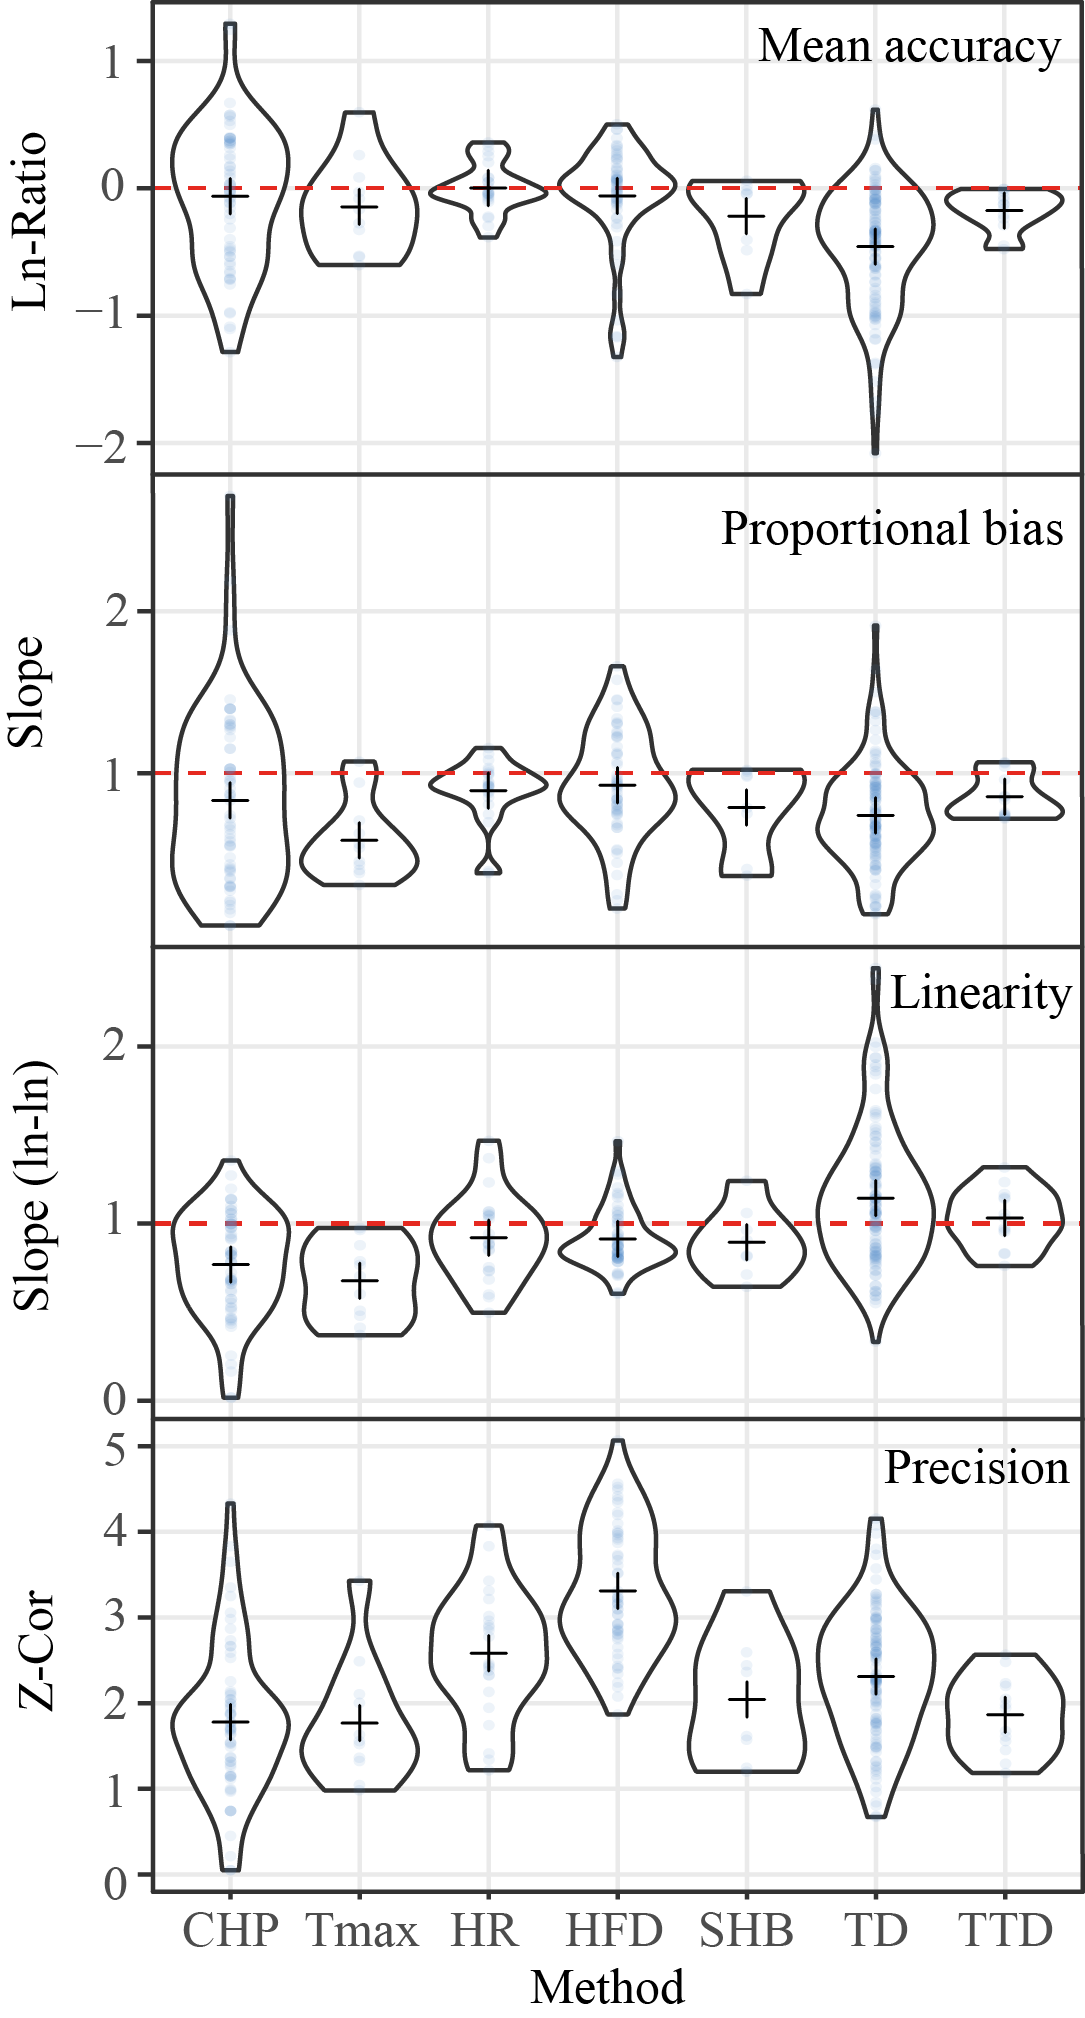
\includegraphics[width=0.55\linewidth]{figure/CH2/Distribution-metrics-orderedV4} 

}

\caption[Distribution of the calibration performance metrics for each method.]{Distribution of the calibration performance metrics for each method. Dots represents the value of each individual calibration metric. Crosses represent the average of the metric for each method. Horizontal, dashed lines specify reference, perfect calibration values for a given metric.}\label{fig:ch2fig2}
\end{figure}
\subsection{Calibration performance compared among methods and families
of
methods}\label{calibration-performance-compared-among-methods-and-families-of-methods}

The average accuracy deviation across sap flow methods (properly
applied) ranged between 14.2\% for CHP and -40.5\% for TD (Table 1.1).
There were significant differences in accuracy (Ln-Ratio) among families
of methods and for methods but not for calibration materials (Fig. 1.3).
The Dissipation family in general and the TD and TTD methods in
particular were the only cases for which the Ln-Ratio was significantly
different from 0 (p\textless{}0.001) (Fig. 1.3), indicating systematic
bias (underestimation).\par

Proportional bias, estimated by Slope, varied among methods and families
of methods (p\textless{}0.01). Among families, Dissipation methods
showed a significantly smaller Slope than Pulse and Field methods (Fig.
1.3(a)), which was largely driven by the low value of TD (Fig. 1.3(b)).
Also, both Pulse and Dissipation families had slopes significantly
different from 1 (p\textless{}0.01 and p\textless{}0.001, respectively),
but only the slope of the TD method was significantly lower than 1
(p\textless{}0.001) (Fig. 1.3). As for the effects of calibration
material, calibrations made with whole plants had a significant
proportional bias (Slope \textless{} 1, p\textless{}0.001) (Fig. 1.3).
\begin{figure}[p]

{\centering 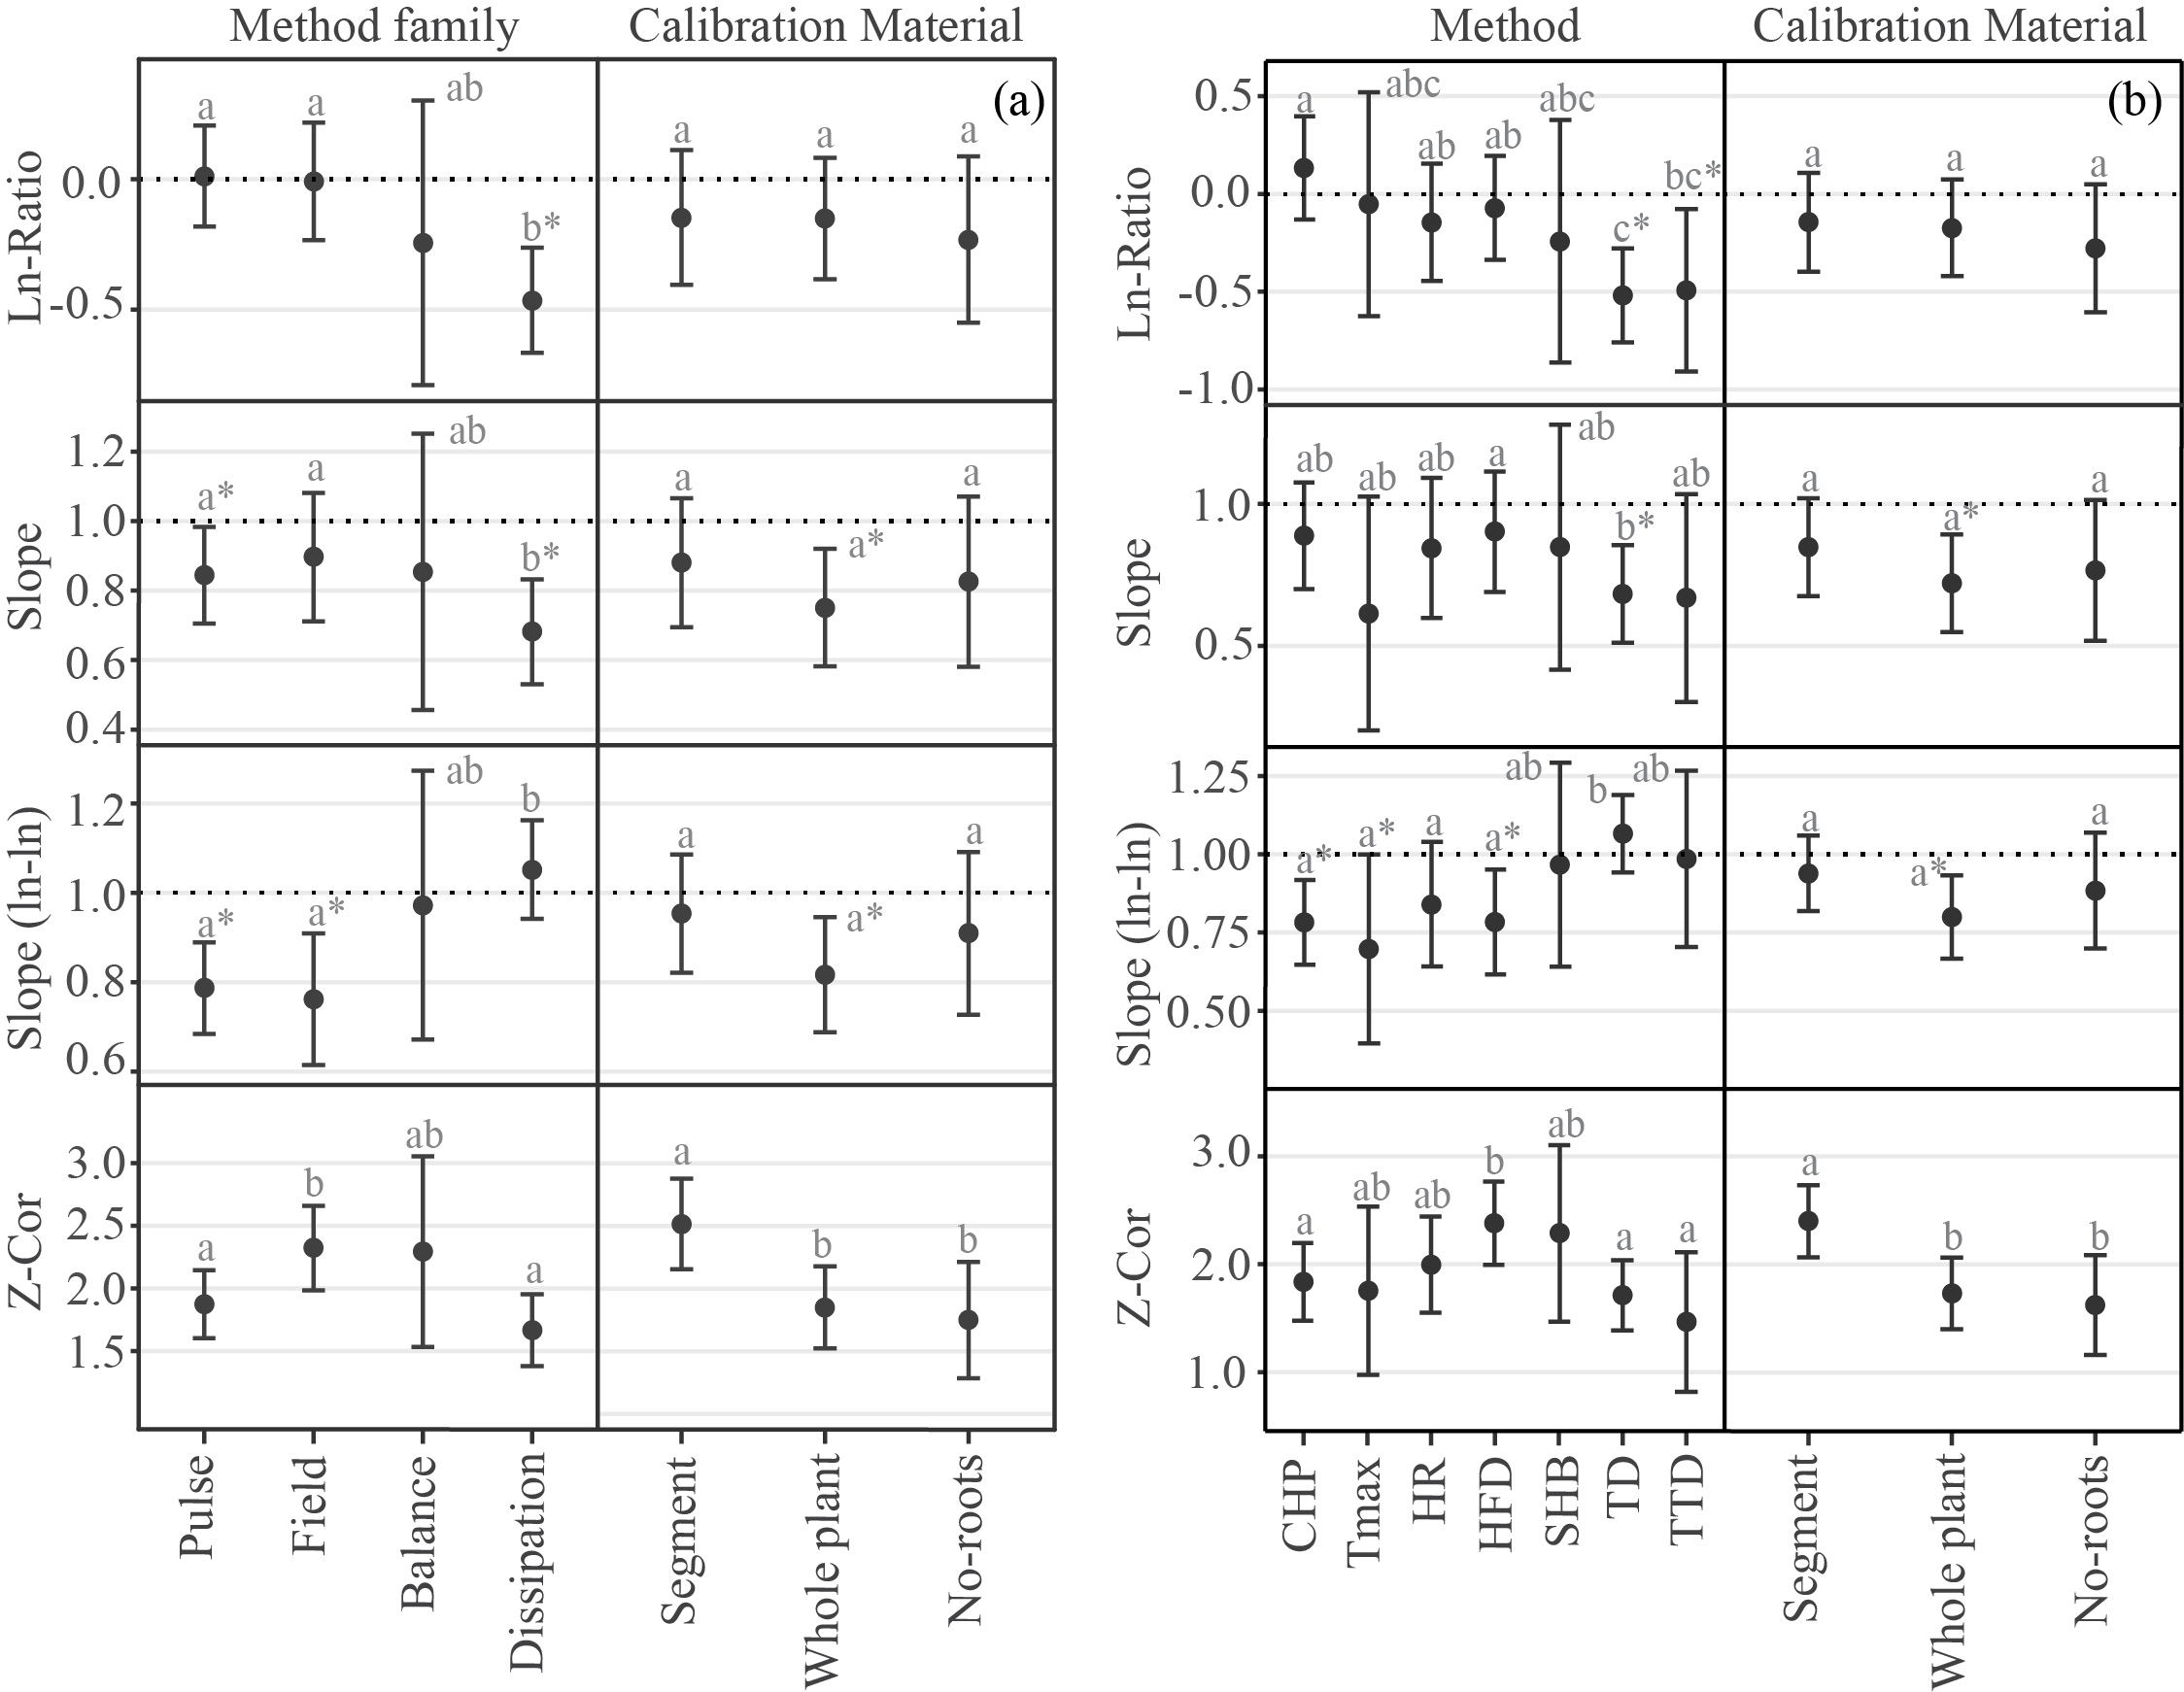
\includegraphics[width=1\linewidth]{figure/CH2/FAMILYMETHODS} 

}

\caption[Predictions of the LMM models of the four calibration metrics.]{Predictions of the LMM models calculated from least-squares means of the four calibration metrics (Ln-Ratio as a proxy for mean accuracy, Slope for proportional bias, Slope (ln-ln) for linearity and Z-Cor for precision) for (a) different families of sap flow methods or for (b) different sap flow methods and for different calibration materials (Segment: stem segment; Whole plant: whole plant on a container or lysimeter; No-roots: whole plant without roots). 95\% confidence intervals of the estimates are also shown. Different letters indicate significant differences between factors levels evaluated with Tukey's test. Horizontal, dotted lines indicate reference, perfect calibration values for a given metric. Asterisks (*) indicate significant departure from those reference values.}\label{fig:ch2fig3}
\end{figure}
Calibration linearity, as denoted by Slope (ln-ln), varied across
methods and families of methods (p\textless{}0.001). We observed higher
values of Slope (ln-ln) for the TD method compared to CHP, T-max, HR and
HFD. Consistently, the Dissipation family in general also had a higher
Slope (ln-ln) than the Pulse and Field families (Fig. 1.3). CHP, T-max
and HFD (and Pulse and Field methods in general) had a Slope (ln-ln)
significantly lower than 1 (Table 1.1 and Fig. 1.3(b)), indicating a
convex relationship between reference and measured flow. Calibrations
performed with whole plants suffered from lack of linearity, indicated
by Slope (ln-ln) significantly lower than 1 (Fig. 1.3).\par

Precision (Z-Cor) was explained by both method and calibration material.
The HFD method (and Field methods in general) provided significantly
higher precision than either Pulse or Dissipation methods (particularly
CHP, TD and TTD) (Table 1.1 and Fig. 1.3(b)). Calibrations performed on
stem segments provided higher precision than those conducted on whole
plants (with or without roots) (Fig. 1.3).\par

In all the previous models, little variability was explained by species
(\(\tau 00\), species), relative to the higher variability associated to
Study, particularly for the Ln-Ratio and Z-Cor models (\(\tau 00\),
study, Table A3). This is consistent with the low ICC values observed
for the species factor, indicating that there is more variability within
than among species (Table A3).\par

In addition, the analysis of the normalized absolute error for the
different methods showed that NRMSE decreased linearly with increasing
measured sap flow in CHP, HFD and TTD methods and increased for T-max,
SHB and TD (Table 1.2 and Fig. A2). For HR the increase in NRMSE with
measured sap flow was not significant. For all the methods that measure
SFD, the absolute error at a typical flow of 25 cm3 cm-2 h-1 ranged
between 6.3 cm3 cm-2 h-1 for CHP and 10.7 cm3 cm-2 h-1 for the TTD
method (Table 1.2).\par
\begin{table}[!h]

\caption[Error analysis of different sap flow methods.]{\label{tab:Ch2T2}Error analysis of different sap flow methods. The normalized root mean square error (NRMSE) is modelled as a function of method and the mean flow range for each calibration (and their interaction) using a LMM model with the same random structure as the main models (cf. section 2.3). $\beta_0$ and $\beta_1$ are the corresponding intercepts and slopes, respectively ($\beta_0$ expressed as \% NRMSE; $\beta_1$ expressed as \% NRMSE per change in $cm^3$ $cm^{-2}$ $h^{-1}$ for SFD or as \% NRMSE per change in $cm^3$ $h^{-1}$ for SF). This linear model, was also used to calculate a reference NRMSE at a sap flux equivalent to the percentile 50 of the range of the data in the calibrations (SFD: 25 $cm^3$ $cm^{-2}$ $h^{-1}$; SF: 1300 $cm^3$ $h^{-1}$). The expected NRMSE and RMSE (in brackets, in $cm^3$ $cm^{-2}$ $h^{-1}$, except for SHB that is in $cm^3$ $h^{-1}$) at a typical flow are also given.}
\centering
\fontsize{10}{12}\selectfont
\begin{tabular}[t]{cccc}
\toprule
\multicolumn{1}{c}{ } & \multicolumn{3}{c}{NRMSE} \\
\cmidrule(l{3pt}r{3pt}){2-4}
Method & $\beta_0$\; \% & $\beta_1$ & reference NRMSE (and RMSE)\\
\midrule
CHP & 27.03*** & -0.08*** & 25.04\% (6.26)\\
T-max & 31.56. & 0.25*** & 37.83\% (9.46)\\
HR & 9.38 & 0.81 & 29.59\% (7.40)\\
HFD & 30.33*** & -0.12*** & 27.45\% (6.86)\\
SHB & 14.85 & 0.02*** & 42.95\% (558.36)\\
TD & 34.93*** & 0.10*** & 37.31\% (9.33)\\
TTD & 44.04*** & -0.04*** & 42.94\% (10.73)\\
\bottomrule
\multicolumn{4}{l}{\textsuperscript{} Statistical significant levels: "." p<0.1 ; "*" p<0.05; "**" p<0.01; "***"}\\
\multicolumn{4}{l}{p<0.001.}\\
\end{tabular}
\end{table}
\subsection{Influence of wood traits}\label{influence-of-wood-traits}

We did not find any significant influence of wood density on accuracy
and linearity metrics (Fig. 1.4). Nonetheless, we observed a negative
effect of wood density on proportional bias of HFD and TD calibrations
(p\textless{}0.05 and p\textless{}0.1, respectively). In addition, a
significant positive effect of wood density on the precision of HFD
measurements was observed (p\textless{}0.001), indicating that the
higher the wood density, the higher the precision (Fig. 1.4).\par

We did not find any significant difference among wood porosity types in
calibration metrics for studies using the TD or CHP methods.
Nevertheless, the non-linearity (Slope (ln-ln) \textless{} 1) observed
in general for the CHP method (Fig. 1.3(b)) was only significant for
species with diffuse-porous wood, not for conifer species (Table
1.3).\par
\begin{figure}[hbt!]

{\centering 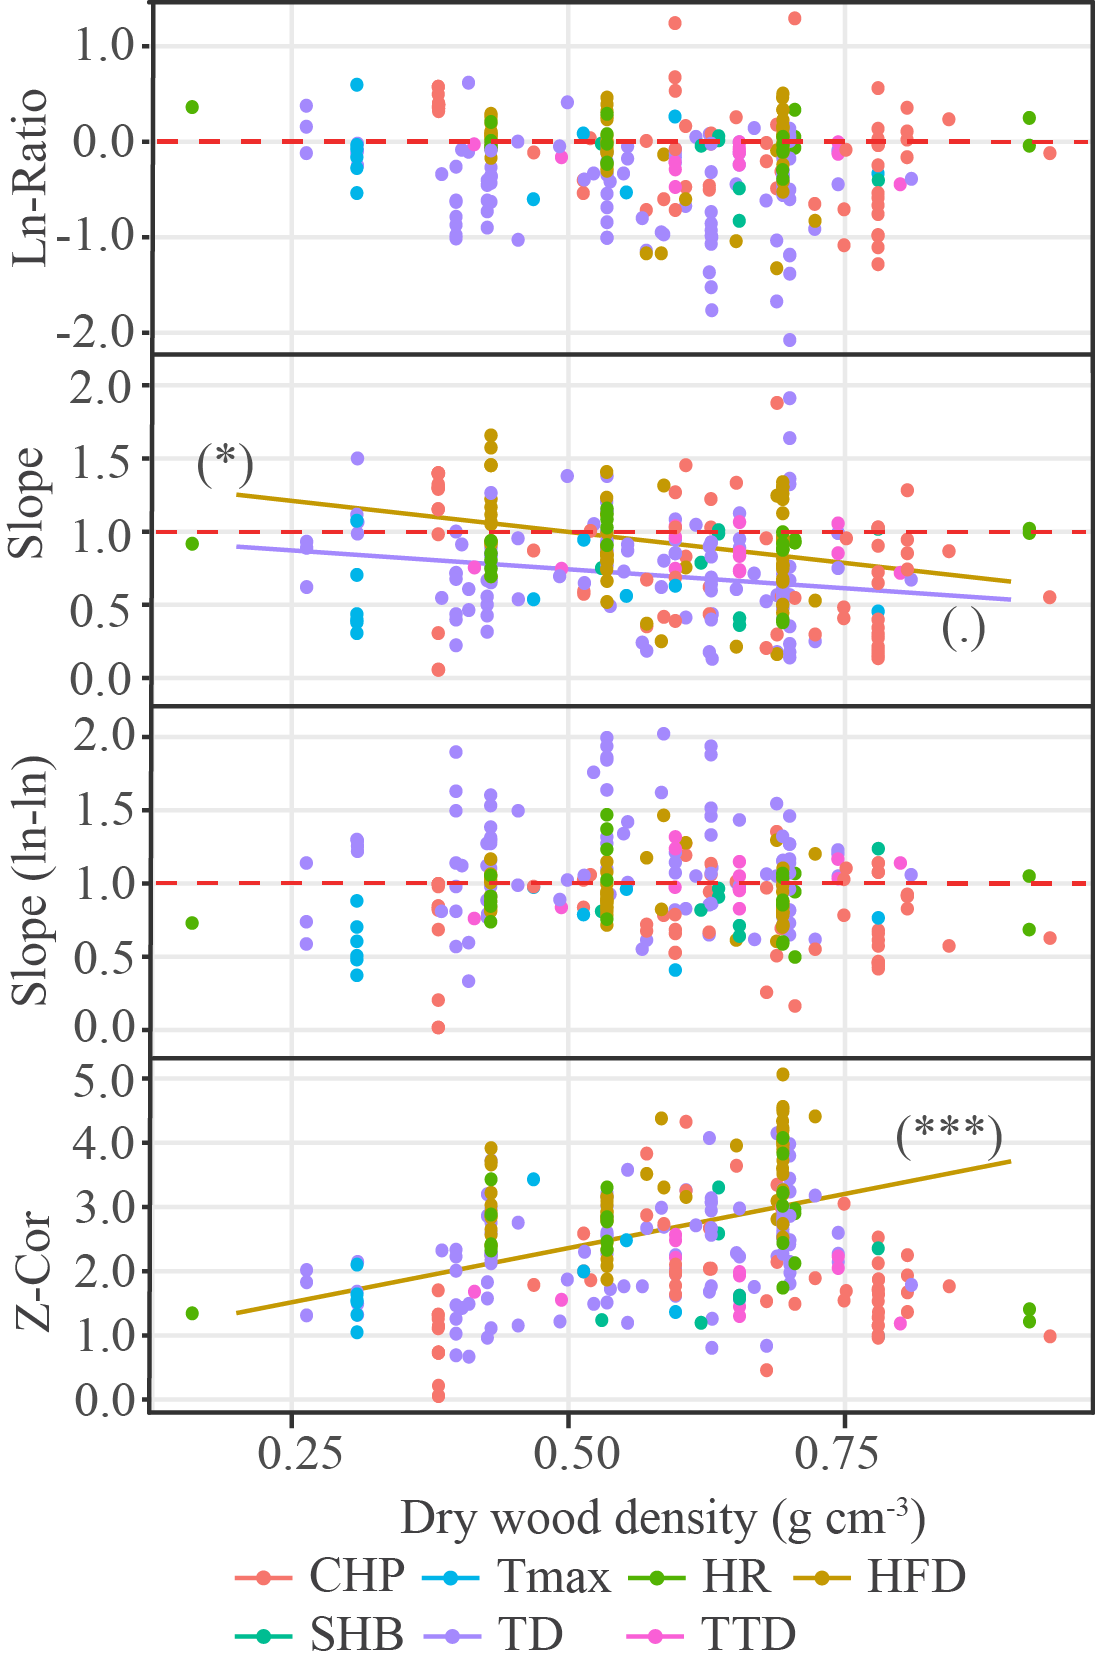
\includegraphics[width=0.55\linewidth]{figure/CH2/DENSITY} 

}

\caption[Relationship between the four calibration performance and wood density, for different sap flow methods.]{Relationship between the four calibration performance metrics (Ln-Ratio as a proxy for accuracy, Slope for proportional bias, Slope (ln-ln) for linearity, and Z-Cor for precision) and wood density, for different sap flow methods. Horizontal, dashed red lines indicate reference, perfect calibration values for a given metric. Regression lines are shown for significant effects only, and the corresponding level of significance (p-value: <0.1: (.), <0.05: (*), < 0.01: (**), < 0.001: (***)) is also reported }\label{fig:ch2fig4}
\end{figure}
\begin{table}

\caption[Least-squares means and 95\% CI calculated from the LMM models testing the effect of different wood porosity types]{\label{tab:Ch2T3}Least-squares means and 95\% CI calculated from the LMM models testing the effect of different wood porosity types (Wood porosity) on sap flow calibration performance metrics (Ln-Ratio as a proxy for accuracy, Slope for proportional bias, Slope (ln-ln) for linearity, and Z-Cor for precision) for CHP and TD methods. No differences were detected among wood anatomies. Significance levels indicate departure from an ideal calibration (Ln-Ratio = 0; Slope = 1; Slope (ln-ln) = 1)}
\centering
\resizebox{\linewidth}{!}{
\fontsize{6}{8}\selectfont
\begin{tabular}[t]{c>{\centering\arraybackslash}p{1.5cm}ccccc}
\toprule
\multicolumn{1}{c}{ } & \multicolumn{1}{c}{ } & \multicolumn{1}{c}{ } & \multicolumn{1}{c}{Accuracy} & \multicolumn{1}{c}{Proportional bias} & \multicolumn{1}{c}{Linearity} & \multicolumn{1}{c}{Precision} \\
\cmidrule(l{3pt}r{3pt}){4-4} \cmidrule(l{3pt}r{3pt}){5-5} \cmidrule(l{3pt}r{3pt}){6-6} \cmidrule(l{3pt}r{3pt}){7-7}
Method & Wood porosity & n & Ln-Ratio & Slope & Slope (ln-ln) & Z-Cor\\
\midrule
CHP & diffuse & 48 & -0.055 [-0.370 , 0.259] & 0.795 [0.557 , 1.033]. & 0.799 [0.671, 0.927] \*\* & 1.980 [1.729 , 2.231]\\
CHP & conifers & 15 & 0.066 [-0.603 , 0.734] & 1.043 [0.459 , 1.627] & 0.777 [0.469 , 1.085] & 1.381 [0.775 , 1.988]\\
TD & diffuse & 81 & -0.273 [-0.658 , 0.111] & 0.752 [0.491 , 1.014]. & 1.126 [0.917 , 1.336] & 1.672 [1.085 , 2.260]\\
TD & ring & 16 & -0.405 [-0.866 , 0.056]. & 0.743 [0.410 , 1.077]. & 0.984 [0.681 , 1.286] & 2.260 [1.572 , 2.947]\\
TD & conifers & 15 & -0.396 [-0.873 , 0.080]. & 0.808 [0.468 , 1.147] & 1.142[0.842 , 1.441] & 1.606 [0.892 , 2.321]\\
\bottomrule
\multicolumn{7}{l}{\textsuperscript{} Statistical significant levels: "." p<0.1 ; "*" p<0.05; "**" p<0.01; "***" p<0.001.}\\
\end{tabular}}
\end{table}
\section{Discussion}\label{discussion}

Our results show a large variability in the quality of sap flow
calibrations, even within the same sap flow method (Fig. 1.2),
highlighting the large variability among and even within studies. This
implies that, even if methods are properly applied (as defined in
section 2.1), sap flow measurements can still produce biased estimates
of water transport rates in plants, and these errors will need to be
considered in quantitative analyses based on this type of measurements.
On average, however, all sap flow methods assessed here produced results
that may be acceptable for qualitative use in most applications, as
shown by the typical high correlation between measured and reference
values (r \textgreater{} 0.89 for all methods and method families, Table
1.1). For quantitative use, no method appears to be suitable for all
experimental contexts, and researchers need to consider both the
inherent limitations of the methods and the need to perform
study-specific calibrations (see Implications and recommendations, Table
1.4).\par

\subsection{Sap flow measurement errors across methods and
methodological
families}\label{sap-flow-measurement-errors-across-methods-and-methodological-families}

A relatively small part of the total variability in the quality of
calibrations is related to methods and families of methods and, to a
lesser extent, to the calibration material (fixed effects explain 8 --
28\% of the variability in calibration metrics; see \(R^2_m\) values in
Table A3). Despite the high variability within methods, we detected
significant differences between methods. Dissipation methods were the
only methods for which accuracy was significantly lower than expected
for an ideal calibration. This is consistent with previous reports
(Braun \& Schmid (1999); S. E. Bush, Hultine, Sperry, Ehleringer, \&
Phillips (2010); Caterina, Will, Turton, Wilson, \& Zou (2014);
({\textbf{???}}); de Oliveira Reis, Campostrini, Sousa, \& Silva (2006);
S. Fuchs et al. (2017); Ping Lu \& Chacko (1998); McCulloh et al.
(2007); Montague \& Kjelgren (2006); Rubilar, Hubbard, Yañez, Medina, \&
Valenzuela (2017); Steppe, De Pauw, Doody, \& Teskey (2010); Taneda \&
Sperry (2008); Uddling, Teclaw, Pregitzer, \& Ellsworth (2009)) and our
synthesis confirms that most of the individual TD and all TTD
calibrations underestimate sap flow systematically (Fig. 1.5).
Interestingly, however, other studies have found the opposite result
(Cain (2009); K. R. Hultine et al. (2010); P Lu (2002); Sperling et al.
(2012); Sun, Aubrey, \& Teskey (2012)) and simulation models (Hölttä,
Linkosalo, Riikonen, Sevanto, \& Nikinmaa (2015); Wullschleger et al.
(2011)) suggest that it is difficult to state a priori whether TD will
over- or underestimate flow, as the measurements obtained are highly
dependent on wood properties and on flux conditions. Our results show
that, globally, the conditions leading to underestimation are more
frequent and support the existence of a proportional bias underlying
this systematic underestimation by TD (Fig. 1.3). It must be also noted,
however, that Dissipation methods have been tested against a much wider
range of flow conditions compared to the rest of the methods (Fig. 1.5,
Fig.6).\par
\begin{table}[!h]

\caption[Synthesis of the potential sources of error and use adequacy for each method.]{\label{tab:Ch2T4}Synthesis of the potential sources of error and use adequacy for each method. Crosses indicates that the method is sensitive to the respective source of error (updated from Vandegehuchte and Steppe, 2013). Methods are classified according to their use effectiveness under different flow conditions: dark grey, light grey and white indicate highly, partially and no recommended use, respectively. When assessing use adequacy for high/low flows, dark and light gray indicate a Normalized Root Mean Square Error (NRMSE) less than a 22\% and a 44\%, respectively, calculated with the NRMSE model (Table 1.2). In Absolute flows use recommendation, dark grey shows methods with both accuracy (Ln-Ratio) and proportional bias (Slope) not significantly different from a perfect calibration. In Relative flows use recommendation, dark grey shows methods with linearity (Slope (ln-ln)) not significantly different from a perfect calibration and with reasonable precision. Potentiality of measuring small stems diameters (< 125mm) is also reported.}
\centering
\fontsize{10}{12}\selectfont
\begin{threeparttable}
\begin{tabular}[t]{cccccccccccccccc}
\toprule
\multicolumn{1}{c}{ } & \multicolumn{9}{c}{Potential source of measure error} & \multicolumn{6}{c}{Effectiveness in measuring} \\
\cmidrule(l{3pt}r{3pt}){2-10} \cmidrule(l{3pt}r{3pt}){11-16}
\rotatebox{90}{\em{Method}} & \rotatebox{90}{\em{Wounding}} & \rotatebox{90}{\em{Radial velocity profile}} & \rotatebox{90}{\em{Wood properties}} & \rotatebox{90}{\em{Natural thermal gradients}} & \rotatebox{90}{\em{Sensor installation}} & \rotatebox{90}{\em{Sensor design}} & \rotatebox{90}{\em{Baselining}} & \rotatebox{90}{\em{Power input}} & \rotatebox{90}{\em{Pulse length}} & \rotatebox{90}{\em{Reverse flows}} & \rotatebox{90}{\em{Low flows*}} & \rotatebox{90}{\em{High flows*}} & \rotatebox{90}{\em{Absolute flows}} & \rotatebox{90}{\em{Relative flows}} & \rotatebox{90}{\em{Small stems}}\\
\midrule
CHP & x & x & x & x & x &  &  &  & x & \multicolumn{1}{c}{\cellcolor[HTML]{FFFFFF}{\textcolor[HTML]{FFFFFF}{0}}} & \multicolumn{1}{c}{\cellcolor[HTML]{BBBBBB}{\textcolor[HTML]{BBBBBB}{1}}} & \multicolumn{1}{c}{\cellcolor[HTML]{999999}{\textcolor[HTML]{999999}{2}}} & \multicolumn{1}{c}{\cellcolor[HTML]{999999}{\textcolor[HTML]{999999}{2}}} & \multicolumn{1}{c}{\cellcolor[HTML]{FFFFFF}{\textcolor[HTML]{FFFFFF}{0}}} & \multicolumn{1}{c}{\cellcolor[HTML]{FFFFFF}{\textcolor[HTML]{FFFFFF}{0}}}\\
T-max & x & x & x &  & x &  & x &  &  & \multicolumn{1}{c}{\cellcolor[HTML]{FFFFFF}{\textcolor[HTML]{FFFFFF}{0}}} & \multicolumn{1}{c}{\cellcolor[HTML]{BBBBBB}{\textcolor[HTML]{BBBBBB}{1}}} & \multicolumn{1}{c}{\cellcolor[HTML]{FFFFFF}{\textcolor[HTML]{FFFFFF}{0}}} & \multicolumn{1}{c}{\cellcolor[HTML]{999999}{\textcolor[HTML]{999999}{2}}} & \multicolumn{1}{c}{\cellcolor[HTML]{FFFFFF}{\textcolor[HTML]{FFFFFF}{0}}} & \multicolumn{1}{c}{\cellcolor[HTML]{FFFFFF}{\textcolor[HTML]{FFFFFF}{0}}}\\
HR & x & x & x &  & x &  &  &  &  & \multicolumn{1}{c}{\cellcolor[HTML]{999999}{\textcolor[HTML]{999999}{2}}} & \multicolumn{1}{c}{\cellcolor[HTML]{999999}{\textcolor[HTML]{999999}{2}}} & \multicolumn{1}{c}{\cellcolor[HTML]{FFFFFF}{\textcolor[HTML]{FFFFFF}{0}}} & \multicolumn{1}{c}{\cellcolor[HTML]{999999}{\textcolor[HTML]{999999}{2}}} & \multicolumn{1}{c}{\cellcolor[HTML]{999999}{\textcolor[HTML]{999999}{2}}} & \multicolumn{1}{c}{\cellcolor[HTML]{999999}{\textcolor[HTML]{999999}{2}}}\\
HFD & x & x &  & x & x & x & x & x &  & \multicolumn{1}{c}{\cellcolor[HTML]{999999}{\textcolor[HTML]{999999}{2}}} & \multicolumn{1}{c}{\cellcolor[HTML]{BBBBBB}{\textcolor[HTML]{BBBBBB}{1}}} & \multicolumn{1}{c}{\cellcolor[HTML]{999999}{\textcolor[HTML]{999999}{2}}} & \multicolumn{1}{c}{\cellcolor[HTML]{999999}{\textcolor[HTML]{999999}{2}}} & \multicolumn{1}{c}{\cellcolor[HTML]{FFFFFF}{\textcolor[HTML]{FFFFFF}{0}}} & \multicolumn{1}{c}{\cellcolor[HTML]{999999}{\textcolor[HTML]{999999}{2}}}\\
SHB &  &  &  & x &  &  & x & x &  & \multicolumn{1}{c}{\cellcolor[HTML]{999999}{\textcolor[HTML]{999999}{2}}} & \multicolumn{1}{c}{\cellcolor[HTML]{999999}{\textcolor[HTML]{999999}{2}}} & \multicolumn{1}{c}{\cellcolor[HTML]{FFFFFF}{\textcolor[HTML]{FFFFFF}{0}}} & \multicolumn{1}{c}{\cellcolor[HTML]{999999}{\textcolor[HTML]{999999}{2}}} & \multicolumn{1}{c}{\cellcolor[HTML]{999999}{\textcolor[HTML]{999999}{2}}} & \multicolumn{1}{c}{\cellcolor[HTML]{999999}{\textcolor[HTML]{999999}{2}}}\\
TD & x & x & x & x &  & x & x & x &  & \multicolumn{1}{c}{\cellcolor[HTML]{FFFFFF}{\textcolor[HTML]{FFFFFF}{0}}} & \multicolumn{1}{c}{\cellcolor[HTML]{BBBBBB}{\textcolor[HTML]{BBBBBB}{1}}} & \multicolumn{1}{c}{\cellcolor[HTML]{BBBBBB}{\textcolor[HTML]{BBBBBB}{1}}} & \multicolumn{1}{c}{\cellcolor[HTML]{FFFFFF}{\textcolor[HTML]{FFFFFF}{0}}} & \multicolumn{1}{c}{\cellcolor[HTML]{999999}{\textcolor[HTML]{999999}{2}}} & \multicolumn{1}{c}{\cellcolor[HTML]{FFFFFF}{\textcolor[HTML]{FFFFFF}{0}}}\\
TTD & x & x & x & x &  & x & x & x &  & \multicolumn{1}{c}{\cellcolor[HTML]{FFFFFF}{\textcolor[HTML]{FFFFFF}{0}}} & \multicolumn{1}{c}{\cellcolor[HTML]{FFFFFF}{\textcolor[HTML]{FFFFFF}{0}}} & \multicolumn{1}{c}{\cellcolor[HTML]{BBBBBB}{\textcolor[HTML]{BBBBBB}{1}}} & \multicolumn{1}{c}{\cellcolor[HTML]{FFFFFF}{\textcolor[HTML]{FFFFFF}{0}}} & \multicolumn{1}{c}{\cellcolor[HTML]{999999}{\textcolor[HTML]{999999}{2}}} & \multicolumn{1}{c}{\cellcolor[HTML]{FFFFFF}{\textcolor[HTML]{FFFFFF}{0}}}\\
\bottomrule
\end{tabular}
\begin{tablenotes}
\small
\item [*] (Low/High: SFD methods: <5 / >80 $cm^{3} cm^{-2} h^{-1}$; SF methods: <260 / >3900 $cm^3 h^{-1}$)
\end{tablenotes}
\end{threeparttable}
\end{table}
Calibration parameters of the TD method were originally considered to be
universal but subsequent studies have claimed that species-specific
calibrations are necessary to obtain correct sap flow measurements (S.
Fuchs et al. (2017); Ping Lu et al. (2004); Steppe et al. (2010)). For a
set of diffuse-porous species, using a pooled calibration also
substantially improved TD (but not HFD) performance compared to
measurements obtained with the original calibration (S. Fuchs et al.
(2017)). However, our results show that species in general and wood
porosity type in particular explain a small or even no proportion of the
variability in the calibrations (Table 1.3 and A3). This implies that
factors related to the experimental context and, possibly, to
intraspecific variability in wood properties (cf.~section 1.5.2) may
have a large contribution to overall uncertainty. Therefore, our results
suggest that calibration parameters for TD or HFD, obtained under
different experimental contexts, may not be generalizable to species
level, as also suggested by Fuchs et al. (2017).\par

In addition to Dissipation methods, Pulse methods also suffer
proportional bias, probably driven by overestimation at low flows,
although this was significant for T-max only (i.e.~positive intercepts
in linear models fitted to calibration data; Fig. 1.5 and 1.6 and A3).
It is well known that the equations of CHP and T-max cannot be solved at
sap flows close to 0, and the calibration intercepts observed here (Fig.
A3) are consistent with the detection thresholds reported for T-max
(\textasciitilde{}10 cm3 cm-2 h-1; Steve Green et al. (2003)) and CHP
(2-4 cm3 cm-2 h-1; T. M. Bleby, Burgess, \& Adams (2004); Steve Green et
al. (2003)). Our results confirm and generalize a previously reported
low-flow detectability problem for T-max (S. Green et al. (2009), Steve
Green et al. (2003); Vandegehuchte \& Steppe (2012b)), but we could not
confirm it for CHP as described before (Barrett et al. (1995); Becker
(1998); T. M. Bleby et al. (2004); Vandegehuchte \& Steppe (2012b)).
Despite overestimation at low flows, the average accuracy of CHP and
T-max is good, which implies that low-flow overestimations may be
compensated with underestimations at high flows. This is also shown by
the lack of linearity observed in both methods (Slope (ln-ln)
\textless{} 1; Fig. 1.3(b)).\par

Our analysis did not detect the saturation effect for the HR method at
high flows that has been reported elsewhere (T. Bleby, McElrone, \&
Burgess (2008); S. Green et al. (2009); Steppe et al. (2015)). This is
likely due to the fact that HR calibrations considered here include few
observations in the region where this overestimation occurs
(\textgreater{} \textasciitilde{}45 cm3 cm-2 h-1; Figs 5 and 6).
Moreover, the high variability in the calibrations probably precluded
detection of the saturation effect (Fig. 1.3 and 1.5) and of the
apparent trend of increasing NRMSE with sap flow range for HR (Table 1.3
and Fig. A2). A lack of linearity can also be observed for HFD,
consistent with the suggested tendency of this method to underestimate
at high flows (Vandegehuchte \& Steppe (2012c)).\par
\begin{figure}[p]

{\centering 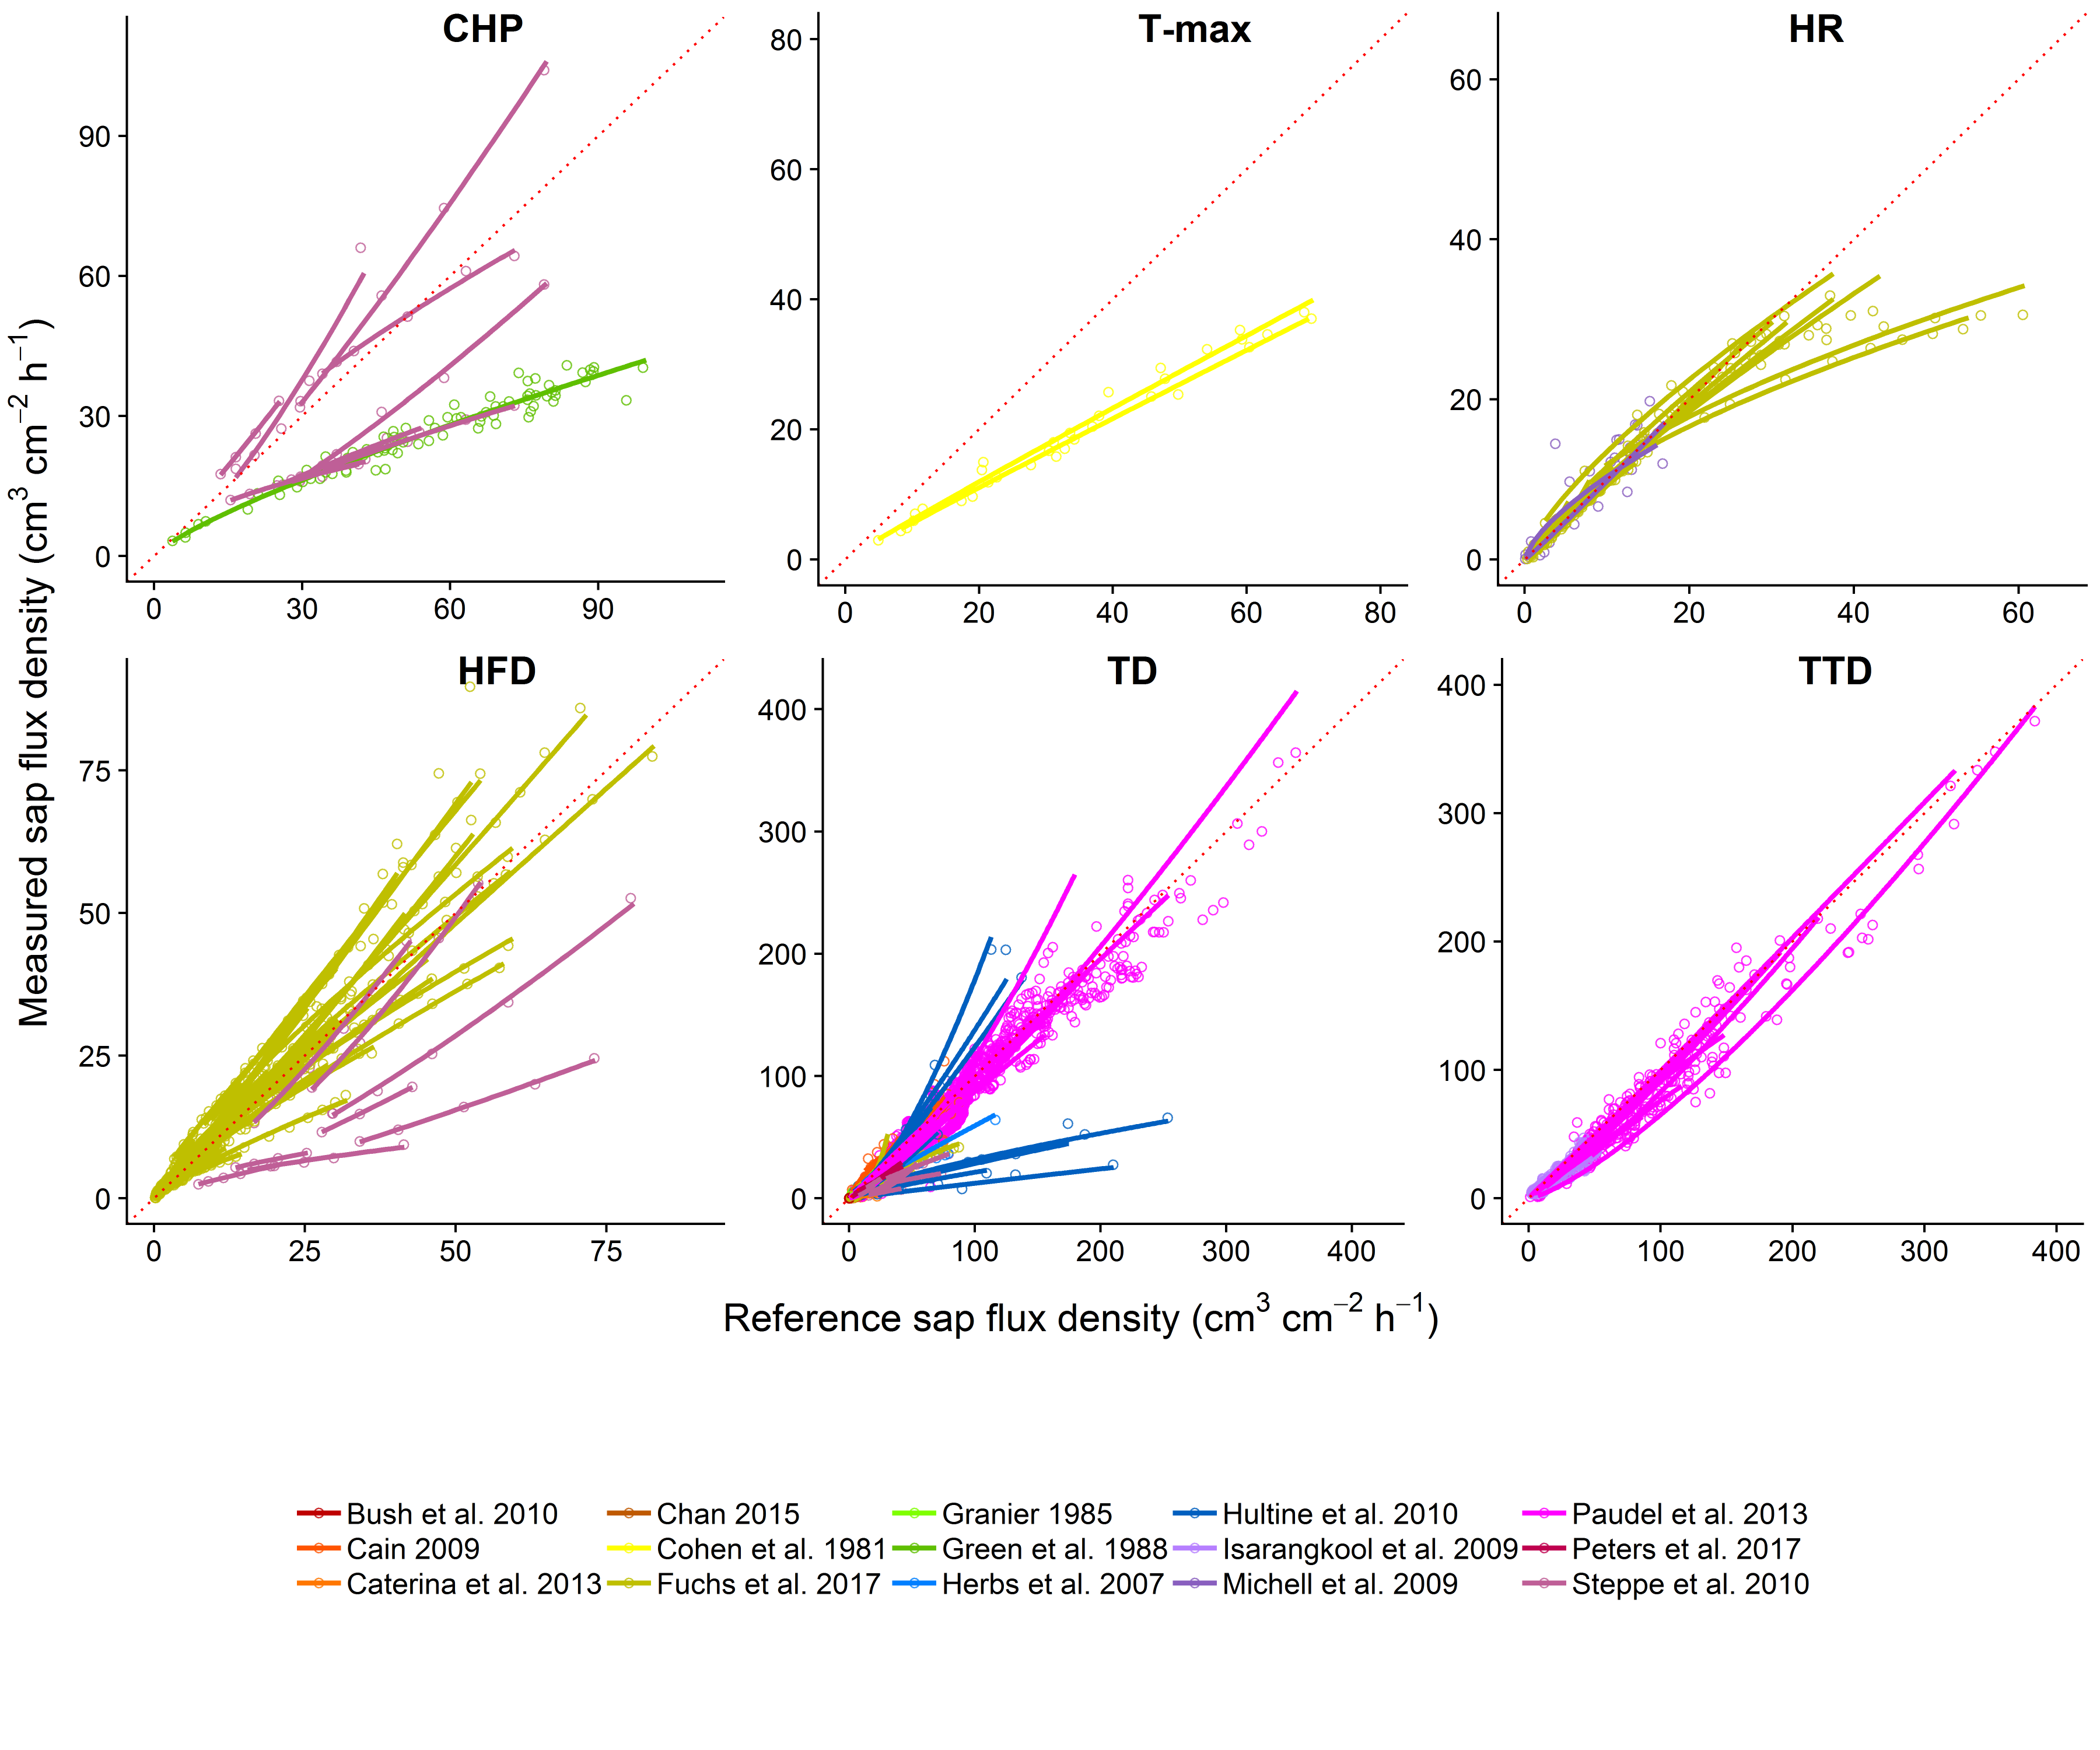
\includegraphics[width=1\linewidth]{figure/CH2/figure-density} 

}

\caption[Relationship between measured and reference sap-flux density (SFD) for different sap flow methods, studies and calibrations.]{Relationship between measured and reference sap-flux density (SFD) for different sap flow methods, studies and calibrations. The fits of ln-ln regressions (Eq. 4) for each calibration are also depicted. Different colors represent different studies that report results in sap-flux density units. Scales vary across panels to facilitate intra method comparison. The red dotted line indicates the 1:1 relationship.}\label{fig:ch2fig5}
\end{figure}
Despite the large variability in precision within methods, our results
show that calibrations performed with HFD give more precise results than
those conducted using the CHP, TD and TTD methods. Although this result
should be interpreted with care as it is based on 57 calibrations but
only from 3 studies, the higher precision observed with HFD could lie in
the second dimension included in the method, which could better capture
the effect of anisotropy of the wood structure. This would also be
consistent with the fact that SHB, a method that is assumed to integrate
sap flow variability within the stem, was the method with the second
highest precision on average, albeit precision was very variable for
this method (Fig. 1.3(b)).\par

We did not detect differences in accuracy, proportional bias or
linearity of the calibrations across calibration materials. However,
compared to an ideal calibration, we did find proportional bias and lack
of linearity in calibrations performed on whole plants, probably because
these calibrations use large scales whose sensitivity and resolution are
usually low, potentially affecting low-flow measurements and leading to
artefactual overestimation at low flows. Poor linearity may also be due
to non-linear changes in belowground hydraulic resistance as the sap
flow increases (J. Martínez-Vilalta, Korakaki, Vanderklein, \&
Mencuccini (2007)). In cut plants, we may have two opposite effects, as
cutting could eliminate belowground resistance (favoring flow) but add
resistance due to putative embolism formation after cutting. Similarly,
the higher precision of calibrations conducted on cut stems relative to
those conducted on whole plants (with and without roots), likely
reflects that cut stem calibrations are normally conducted in
laboratories with precision scales and under controlled conditions that
minimize experimental random errors.\par
\begin{figure}[p]

{\centering 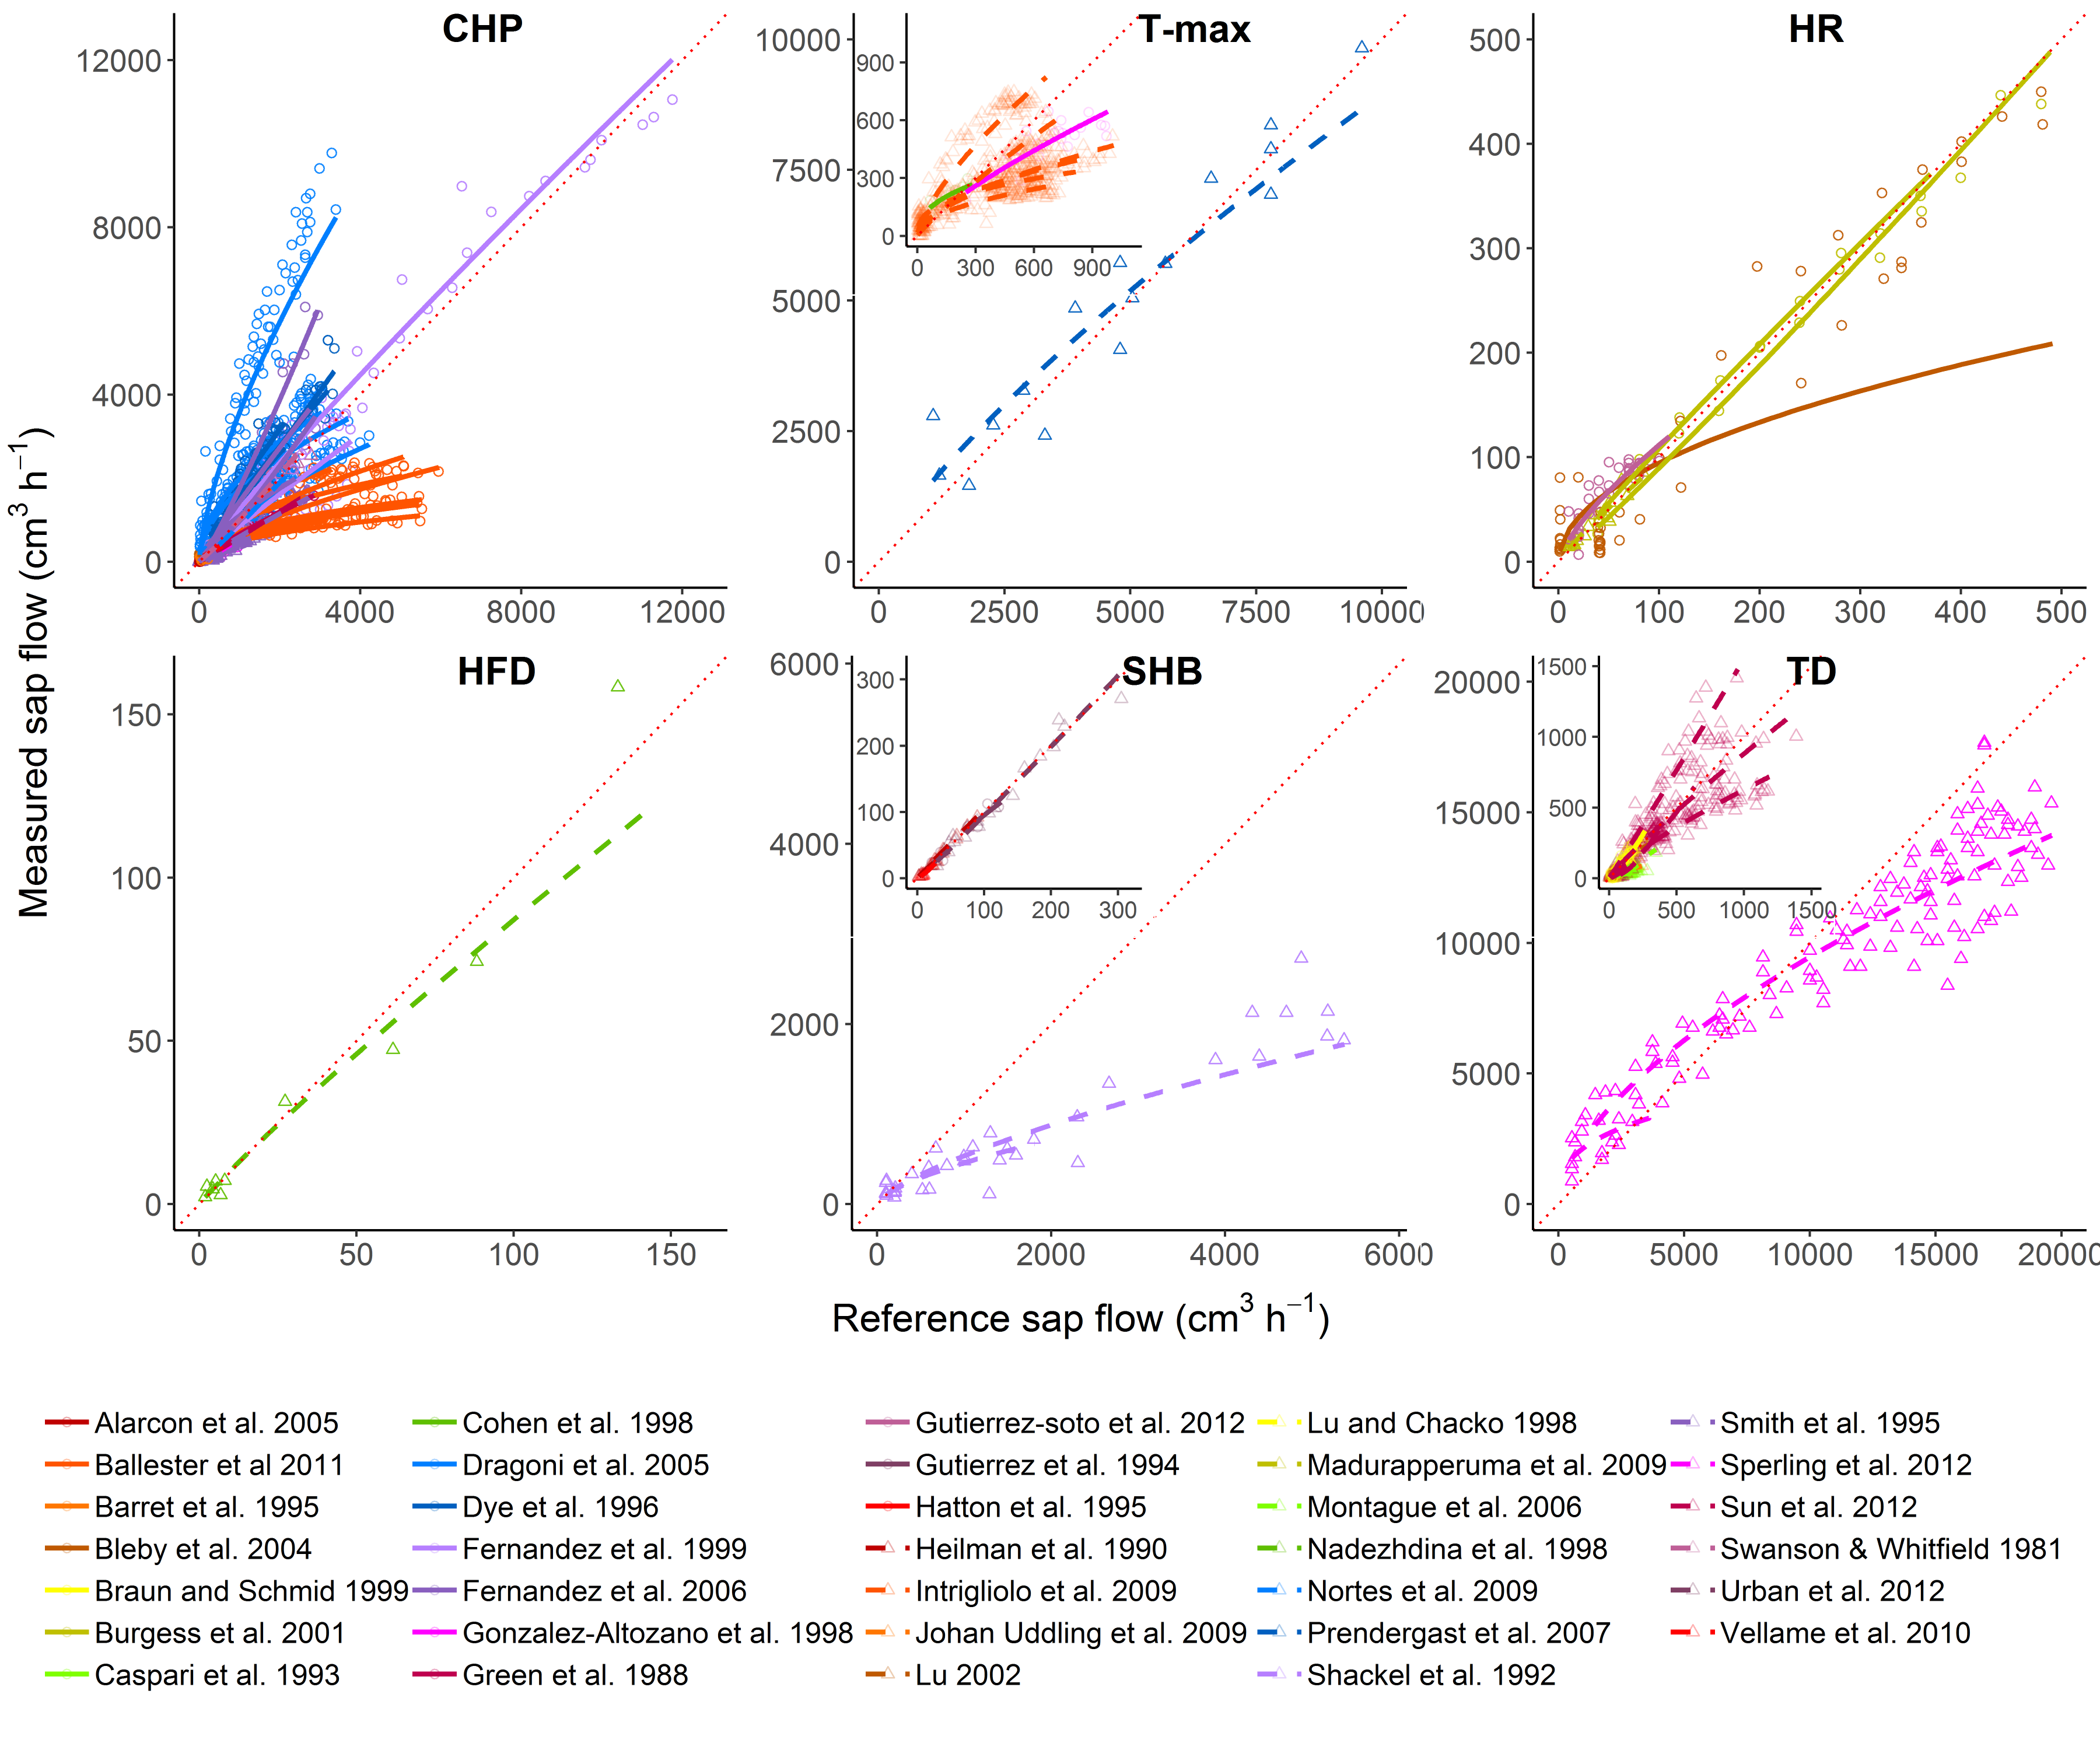
\includegraphics[width=1\linewidth]{figure/CH2/figure-totalflow} 

}

\caption[Relationship between measured and reference sap flow (SF) for different sap flow methods, studies and calibrations.]{Relationship between measured and reference sap flow (SF) for different sap flow methods, studies and calibrations. The fits of ln-ln regressions (Eq. 4) for each calibration are also depicted. Different color symbols and line types represent different studies. Scales varies across panels to facilitate intra method comparison. Insets are shown in some panels (T-max, SHB, TD) to facilitate visualization when the flow ranges differed markedly among calibrations for the same method. The red dotted line indicates 1:1 relationship.}\label{fig:ch2fig6}
\end{figure}
\subsection{The performance of sap flow calibrations is largely
unrelated to species wood
traits}\label{the-performance-of-sap-flow-calibrations-is-largely-unrelated-to-species-wood-traits}

Species-specific wood density and wood porosity type explained little
variability in overall calibration performance, although we detected
some effects of wood density for HFD and TD calibrations. Wood density
affected HFD measurements by increasing precision, which could be
related to the response time of the sensors. If we assume that maximum
sapwood water content is reduced as wood density increases (Simpson
(1993)), associated changes in thermal diffusivity could lead to a
faster sensor response (Hölttä et al. (2015)), higher correlation
between actual and measured flows. Wood density also showed a negative
relationship with proportional bias for HFD and TD, a pattern that could
be caused by the combined effects of wood density and water content on
wood thermal diffusivity (Vandegehuchte \& Steppe (2012c); Vergeynst et
al. (2014)). The fact that we did not find clear effects of wood density
on calibration accuracy and linearity, despite that wood density affects
thermal diffusivity and hence heat transport (Wullschleger et al.
(2011)), could be explained by two reasons. Firstly, we could not use
the actual wood density for most of the calibrations, because it was not
reported in the corresponding studies, and using species-level averages
instead of the wood density of the plant material specifically used on
the calibrations may mask the effect of wood density on calibration
performance. Secondly, wood density in angiosperms appears to be only
weakly correlated to some wood properties that could be important for
sap flow calibrations, such as lumen fraction (Zanne et al. (2010)).\par

Our global analysis did not show clear and consistent differences in
calibration quality between different wood porosity types (Table 1.2) as
previously suggested by several studies for both CHP (S. R. Green \&
Clothier (1988)) and TD methods (S. E. Bush et al. (2010); Sun et al.
(2012)). According to heat transport theory, we should expect declining
performance from conifer to ring-porous species (i.e.~from most
homogenous to most heterogeneous wood). For CHP, we found that
proportional bias (only marginally) and nonlinearity departed from an
ideal calibration for diffuse-porous species, but these patterns did not
differ significantly from those observed for conifers. Our results did
not clearly support either an inferior performance of TD in ring-porous
species compared to diffuse-porous or conifers, as could be expected
from the reported underestimation driven by large sap flow gradients
along sensor length or by the imperfect probe contact with hydroactive
xylem in species with narrow sapwood (Michael J Clearwater et al.
(1999); but see Wullschleger et al. (2011)). Wood porosity effects on
sap flow calibrations have been inferred in individual studies from
measurements in few species representative of each wood porosity type
(S. E. Bush et al. (2010); Sun et al. (2012); Xie \& Wan (2018)) and our
inability to detect these effects here may be caused by the high
variability in experimental context within our dataset. Furthermore, the
effect of the different anatomies may be masked by high structural
variability within wood porosity types, as for example the variation in
latewood to earlywood in conifers (Fan, Guyot, Ostergaard, \& Lockington
(2018)) and we cannot discard that calibration performance could be
related to quantitative anatomical traits not assessed in this study
(cf. Xie \& Wan (2018)). Although the low variability we observed at the
species level suggests that quantitative anatomical traits might not
explain much of the variability in sap flow calibrations, we encourage
that quantitative wood traits are measured in the same plant material
used to calibrate sap flow sensors to better understand the influence of
wood properties on the variability of sap flow calibrations.\par

\subsection{Implications and
recommendations}\label{implications-and-recommendations}

Our global analysis shows that even when the methods are applied
following standard recommendations the quality of individual
calibrations can be very low (Fig. 1.3). This result reflects, on one
hand, systematic bias in TD and lack of linearity in CHP, two of the
most widely used methods (Fig. A1) and, on the other hand, unknown
sources of error related to experimental conditions and/or sample
characteristics (Table 1.4). In our study, we could not account for all
the experimental conditions to evaluate these sources of variability,
except for the effect of the calibration material. Examples of factors
that may affect calibrations when using the same type of calibration
material include sensor design (S. Fuchs et al. (2017)), sensor
installation (T. M. Bleby et al. (2004); Ping Lu \& Chacko (1998); Ren
et al. (2017)), variation in calculations of wood thermal properties
(Looker et al. (2016)), zero flow determination (Looker et al. (2016);
Peters et al. (2018)) or the mechanism of flow generation in cut stem
calibrations (negative vs positive pressures) (S. Fuchs et al. (2017))
(Table 1.4). Previous reports, however, usually focus on only one of the
sources of experimental error. Importantly, relevant methodological
information that could be used to assess (and account for) these sources
of error is frequently not reported (Peters et al. (2018); Steppe et al.
(2015)). Clearly, further research into the effects of experimental
conditions on the quality of different sap flow methods should be a
priority, as well as more complete, standardized reporting of
experimental conditions, including information on the sources of
potential methodological errors listed in Table 1.4.\par

Our results show that calibrations may be needed to obtain correct
absolute values of sap flow, even when Pulse methods are used (see also
S. Fuchs et al. (2017); Steppe et al. (2010)). However, sap flow
calibrations provide a snapshot of the performance of a given sap flow
method under relatively stable conditions, which may greatly differ from
those experienced by plants in the field. Moreover, our analysis could
not address the methodological variability related to more dynamic
effects such as errors caused by changes in sapwood water content
(Vergeynst et al. (2014)), long-term wounding or signal dampening
(Maranon-jimenez2018; Peters et al. (2018); A Wiedemann et al. (2013)).
In this sense, more studies should assess calibration applicability to
mid- or long-term measurements (e.g., Oliveras \& Llorens (2001)),
possibly combined with independent estimates of sapwood water content
(Vandegehuchte \& Steppe (2012b)) and whether calibrations obtained from
excised segments are valid for whole-plants.\par

Considering only their performance in calibration tests (i.e.~no other
logistic or technical issues, such as sensor, datalogging, or power
constraints, which will be study-specific) we can provide some general
recommendations on the use of sap flow methods (Table 1.4). The most
widely used method, TD, appears to be consistently inaccurate, shows
proportional bias and generally underestimates sap flow, by 40\% on
average (if used with its original calibration coefficients). However,
it presents good linearity, which implies that this method can be used
when sap flow responses to environmental variables and/or treatments are
the primary focus of the study (i.e., good estimates of absolute sap
flow values are not critical). In comparison, CHP, T-max and HFD all
present a certain nonlinearity which may affect the estimation of these
environmental responses. At least for CHP and T-max (specially for the
latter) this pattern seems to be driven by overestimation at low flows
and underestimation at high flows canceling out each other. This implies
that both Pulse methods could be suitable for studies interested in
absolute values of transpiration. For the HFD method, the nonlinearity
could be influencing the estimations of radial sap flow patterns, as
these measurements would need to correctly measure both high and low
flows simultaneously. We also confirm that the HR method may not be
suitable to measure high flows but it is probably the best method for
detailed physiological studies involving low flows.\par

\section{Conclusions}\label{conclusions}

In conclusion, our global assessment contributes towards a proper
incorporation of measurement errors in the interpretation of individual
case studies and in modelling studies aimed at upscaling sap flow data
(T. J. Hatton et al. (1995); Hernandez-Santana et al. (2015)). Perhaps
even more importantly, it paves the way towards improved intercomparison
of sap flow datasets obtained with different methods to assess regional
or global patterns in plant water use (e.g., the SAPFLUXNET initiative;
Poyatos et al. (2016)). Although providing explicit correction factors
for each method is beyond the scope of this paper, the typical accuracy
deviations provided in Table 1.1 can be used as a first order correction
when combining sap flow data from different methods (and no additional
information on study-specific uncertainty sources is available).\par

\chapter[The SAPFLUXNET database]{Global transpiration data from sap flow measurements: the SAPFLUXNET database}

\setlength{\parskip}{0.2cm plus4mm minus3mm} \setlength{\parindent}{0pt}
Rafael Poyatos, Víctor Granda, Víctor Flo, Jordi Martínez-Vilalta
\emph{et al}. \newpage
\setlength{\parindent}{30pt}

\section*{Abstract}

lant transpiration links physiological responses of vegetation to water
supply and demand with hydrological, energy and carbon budgets at the
land-atmosphere interface. However, despite being the main land
evaporative flux at the global scale, transpiration and its response to
environmental drivers are currently not well constrained by
observations. Here we introduce the first global compilation of
whole-plant transpiration data from sap flow measurements (SAPFLUXNET,
\url{https://sapfluxnet.creaf.cat/}). We harmonised and
quality-controlled individual datasets supplied by contributors
worldwide in a semi-automatic data workflow implemented in the R
programming language. Datasets include sub-daily time series of sap flow
and hydrometeorological drivers for one or more growing seasons, as well
as metadata on the stand characteristics, plant attributes and technical
details of the measurements. SAPFLUXNET contains 202 globally
distributed datasets with sap flow time series for 2714 plants, mostly
trees, of 174 species. SAPFLUXNET has a broad bioclimatic coverage, with
woodland/shrubland and temperate forest biomes especially
well-represented (80\% of the datasets). The measurements cover a wide
variety of stand structural characteristics and plant sizes. The
datasets encompass the period between 1995 and 2018, with 50\% of the
datasets being at least 3 years long. Accompanying radiation and vapour
pressure deficit data are available for most of the datasets, while
on-site soil water content is available for 56\% of the datasets. Many
datasets contain data for species that make up 90\% or more of the total
stand basal area, allowing the estimation of stand transpiration in
diverse ecological settings. SAPFLUXNET adds to existing plant trait
datasets, ecosystem flux networks and remote sensing products to help
increase our understanding of plant water use, plant responses to
drought and ecohydrological processes. SAPFLUXNET version 0.1.5 is
freely available from the Zenodo repository
(\url{https://doi.org/10.5281/zenodo.3971689}, Poyatos et al. 2020a).
The `sapfluxnetr' R package, designed to access, visualise and process
SAPFLUXNET data is available from CRAN.\par

\newpage

\section{Introduction}\label{introduction}

Terrestrial vegetation transpires ca. 45000 km3 of water per year
(Schlesinger and Jasechko, 2014; Wang-Erlandsson et al., 2014; Wei et
al., 2017), a flux that represents 40\% of global land precipitation,
70\% of total land evapotranspiration (Oki and Kanae, 2006), and is
comparable in magnitude to global annual river discharge (Rodell et al.,
2015). For most terrestrial plants, transpiration is an inevitable water
loss to the atmosphere because they need to open stomata to allow CO2
diffusion into the leaves for photosynthesis. Latent heat from
transpiration represents 30--40\% of surface net radiation globally
(Schlesinger and Jasechko, 2014; Wild et al., 2015). Transpiration is
therefore a key process coupling land-atmosphere exchange of water,
carbon and energy, determining several vegetation-atmosphere feedbacks,
such as land evaporative cooling or moisture recycling. Regulation of
transpiration in response to fluctuating water availability and/or
evaporative demand is a key component of plant functioning and one of
the main determinants of a plant's response to drought (Martin‐StPaul et
al., 2017; Whitehead, 1998). Despite its relevance for earth
functioning, transpiration and its spatiotemporal dynamics are poorly
constrained by available observations (Schlesinger and Jasechko, 2014)
and not well represented in models (Fatichi et al., 2016; Mencuccini et
al., 2019). An improved understanding on how plants regulate
transpiration is thus needed to better predict future trajectories of
land evaporative fluxes and vegetation functioning under increased
drought conditions driven by global change.\par

Conceptually, transpiration can be quantified at different
organisational scales: leaves, branches and whole plants, ecosystems and
watersheds. In practice, transpiration is relatively easy to isolate
from the bulk evaporative flux, evapotranspiration, only from the leaf
to the plant levels. In terrestrial ecosystems, evapotranspiration
includes evaporation from the soil and from water-covered surfaces,
including plants. Transpiration measurements on individual leaves or
branches with gas exchange systems are difficult to upscale to the plant
level (Jarvis, 1995). Likewise, transpiration measurements using
whole-plant chambers (e.g.~Pérez-Priego et al., 2010) or gravimetric
methods (e.g.~weighing lysimeters) in the field are still challenging.
At the ecosystem scale and beyond, evapotranspiration is generally
determined using micrometeorological methods, catchment water budgets or
remote sensing approaches (Shuttleworth, 2007; Wang and Dickinson,
2012). In some cases, isotopic methods and different algorithms applied
to measured ecosystem fluxes can provide an estimation of transpiration
at the ecosystem scale (Kool et al., 2014; Stoy et al., 2019).\par

Transpiration drives water transport from roots to leaves in the form of
sap flow through the plant's xylem pathway (Tyree and Zimmermann, 2002),
and this sap flow affects heat transport in the xylem. Taking advantage
of this, thermometric sap flow methods were first developed in the 1930s
(Huber, 1932) and further refined over the following decades (Čermák et
al., 1973; Marshall, 1958) to provide operational measurements of plant
water use. These methods have become widely used in plant ecophysiology,
agronomy and hydrology (Poyatos et al., 2016), especially after the
development of simple, easily replicable methods (e.g.~Granier, 1985,
1987). Whole-plant measurements of water use using thermometric sap flow
methods provide estimates of water flow through plants from sub-daily to
interannual timescales, and have been mostly applied in woody plants
(but see Baker and Van Bavel (1987) for measurements on herbaceous
species). Xylem sap flow is measured semi-invasively (Brodersen et al.,
2019) and can be upscaled to the whole plant, obtaining a
near-continuous quantification of plant water use. Multiple sap flow
sensors can be deployed, in almost any terrestrial ecosystem, to
determine the magnitude and temporal dynamics of transpiration across
species, environmental conditions or experimental treatments. All sap
flow methods are subject to methodological and scaling issues, which may
affect the quantification of absolute water use in some circumstances
(Čermák et al., 2004; Köstner et al., 1998; Smith and Allen, 1996;
Vandegehuchte and Steppe, 2013). Nevertheless, all methods are suitable
for the assessment of the temporal dynamics of transpiration and of its
responses to environmental changes or to experimental treatments (Flo et
al., 2019).\par

The generalised application of sap flow methods in ecological and
hydrological research in the last 30 years has thus generated a large
volume of data, with an enormous potential to advance our understanding
of the spatiotemporal patterns and the ecological drivers of plant
transpiration and its regulation (Poyatos et al., 2016). However, this
large volume of data needs to be compiled and harmonised to enable
global syntheses and comparative studies across species and regions.
Across-species data syntheses using sap flow data have mostly focused on
maximum values extracted from publications (Kallarackal et al., 2013;
Manzoni et al., 2013; Wullschleger et al., 1998). Multi-site syntheses
have focused on the environmental sensitivity of sap flow, using site
means of plant-level sap flow or sap flow-derived stand transpiration
(Poyatos et al., 2007; Tor‐ngern et al., 2017). Since data sharing is
only incipient in plant ecophysiology, sap flow datasets have not been
traditionally available in open data repositories. Open data practices
are now being implemented in databases, which fosters collaboration
across monitoring networks in research areas relevant to plant
functional ecology (Falster et al., 2015; Gallagher et al., 2020; Kattge
et al., 2020) and ecosystem ecology (Bond-Lamberty and Thomson, 2010).
The success of the data sharing and data re-use policies within the
FLUXNET global network of ecosystem level fluxes has shown how these
practices can contribute to scientific progress (Bond‐Lamberty,
2018).\par

Here we introduce SAPFLUXNET, the first global database of sap flow
measurements built from individual community-contributed datasets. We
implemented this compilation in a data structure designed to accommodate
time series of sap flow and the main hydrometeorological drivers of
transpiration, together with metadata documenting different aspects of
each dataset. We harmonised all datasets and performed basic
semi-automated quality assurance and quality control procedures. We also
created a software package that provides access to the database, allows
easy visualisation of the datasets and performs basic temporal
aggregations. We present the ecological and geographic coverage of
SAPFLUXNET version 0.1.5, (Poyatos et al., 2020a) followed by a
discussion of potential applications of the database, its limitations
and a perspective of future developments. \par

\section{The SAPFLUXNET data
workflow}\label{the-sapfluxnet-data-workflow}

\subsection{An overview of sap flow
measurements}\label{an-overview-of-sap-flow-measurements}

The main characteristics of sap flow methods have been reviewed
elsewhere (Čermák et al., 2004; Smith and Allen, 1996; Swanson, 1994;
Vandegehuchte and Steppe, 2013). Given the already broad scope of the
paper, here we only provide a brief methodological overview, without
delving into the details of the individual methods. Sap flow sensors
track the fate of heat applied to the plant's conducting tissue, or
sapwood, using temperature sensors (thermocouples or thermistors),
usually deployed in the plant's main stem. Both heating and temperature
sensing can be done either internally, by inserting needle-like probes
containing electrical resistors (or electrodes for some methods) and
temperature sensors into the sapwood, or externally; these latter
systems being especially designed for small stems. Depending on how the
heat is applied and the principles underlying sap flow calculations, sap
flow sensors can be classified into three major groups: heat dissipation
methods, heat pulse methods and heat balance methods (Flo et al., 2019).
Heat dissipation and heat pulse methods estimate sap flow per unit
sapwood area and they have been called `sap flux density methods'
(Vandegehuchte and Steppe, 2013); heat balance methods directly yield
sap flow for the entire stem or for a sapwood section. Heat dissipation
methods include the constant heat dissipation (HD; Granier 1985, 1987),
the transient (or cyclic) heat dissipation (CHD; Do and Rocheteau, 2002)
and the heat deformation (HFD; Nadezhdina 2018) methods. Heat pulse
methods include the compensation heat pulse (CHP; Swanson and Whitfield,
1981), heat ratio (HR; Burgess et al. 2001), T-max (HPTM; Cohen et al.
1981) and Sapflow+ (Vandegehuchte and Steppe, 2012) methods. Heat
balance methods include the trunk sector heat balance (TSHB; Čermák et
al. 1973) and the stem heat balance (SHB; Sakuratani, 1981) methods. The
suitability of a certain method in a given application largely depends
on plant size and the flow range of interest (Flo et al., 2019), but HD
and CHP are the most widely used (Flo et al., 2019; Peters et al., 2018;
Poyatos et al., 2016). Apart from these different methodologies, within
each sap flow method variants exist in sensor design and in data
processing approaches, resulting in relatively high levels of
methodological uncertainty comparable to those in other areas of plant
ecophysiology.\par

The output from sap flow sensors is automatically recorded by
dataloggers, at hourly or even higher temporal resolution. This output
relates to heat transport in the stem and needs to be converted to
meaningful quantities of water transport, such as sap flow per plant or
per unit sapwood area. How this conversion is achieved varies greatly
across methods, with some relying on empirical calibrations and others
being more physically-based and requiring the estimation of wood thermal
properties and other parameters (Čermák et al., 2004; Smith and Allen,
1996; Vandegehuchte and Steppe, 2013). Depending on the method and the
specific sensor design, sap flow measurements can be representative of
single points, linear segments along the sapwood, sapwood area sections
or entire stems. Except for stem heat balance methods, these
measurements need to be spatially integrated to account for radial
(Berdanier et al., 2016; Cohen et al., 2008; Nadezhdina et al., 2002;
Phillips et al., 1996) and azimuthal (Cohen et al., 2008; Lu et al.,
2000; Oren et al., 1999a) variation of sap flow within the stem to
obtain an estimate of whole-plant water use (Čermák et al., 2004). At a
minimum, an estimate of sapwood area is needed to upscale the
measurements to whole-plant sap flow rates. Sap flow rates can thus be
expressed per individual (i.e.~plant or tree), per unit sapwood area
(normalising by water-conducting area), and per unit leaf area
(normalising by transpiring area).\par

Here we will use the term `sap flow' when referring, in general, to the
rate at which water moves through the sapwood of a plant and, more
specifically, when we refer to sap flow per plant (i.e.~water volume per
unit time, Edwards et al., 1996). We acknowledge that the term `sap
flux' has also been proposed for this quantity (Lemeur et al., 2009),
but more generally, `sap flux density' (e.g.~Vandegehuchte and Steppe,
2013) or just `sap flux' are used to refer to `sap flow per unit sapwood
area'. Since here we include methods natively measuring sap flow per
plant or per sapwood area, throughout this paper we will use the more
general term `sap flow', and, when necessary, we will indicate
explicitly the reference area used: `sap flow per (unit) sapwood area',
`sap flow per (unit) leaf area' or `sap flow per (unit) ground
area'.\par 

\subsection{Data compilation}\label{data-compilation}

SAPFLUXNET was conceived as a compilation of published and unpublished
sap flow datasets (Appendix Table A1) and thus the ultimate success of
the initiative critically depended on the contribution of datasets by
the sap flow community. An expression of interest showed that a critical
mass of datasets with a wide geographic distribution could potentially
be contributed and the results of this survey were used to raise the
interest of the sap flow community (Poyatos et al., 2016). The data
contribution stage was open between July 2016 and December 2017 although
a few additional datasets were updated during the data quality control
process and contain more recent data. \par

All contributed datasets had to meet some minimum criteria before they
were accepted, both in terms of content and format. We required that all
datasets contained sub-daily, processed sap flow data, representative of
whole-plant water use under different hydrometeorological conditions.
This meant that both the processing from raw temperature data to sap
flow quantities and the scaling from single-point measurements to
whole-plant data had been performed by the data contributor responsible
for each dataset. Time-series of sap flow data and hydrometeorological
drivers were required to be representative of one growing-season,
setting, as broad reference, a minimum duration of 3 months. Sap flow
could be either expressed as total flow rate per plant or per unit
sapwood area. Contributors also needed to provide metadata on relevant
ecological information of the site, stand, species and measured plants
as well as on basic technical details of the sap flow and
hydrometeorological time-series. Datasets had to be formatted using a
documented spreadsheet template (cf.
`sapfluxnet\_metadata\_template.xlsx' in the Supplement) and uploaded to
a dedicated server at CREAF, Spain, using an online form.\par

\subsection{Data harmonisation and quality control:
QC1}\label{data-harmonisation-and-quality-control-qc1}

Once datasets were received, they were stored and entered a process of
data harmonisation and quality control (Fig. 1, Supplement Fig. S1).
This process combined automatic data checks with human supervision, and
the entire workflow was governed by functions and scripts in the R
language (R Core Team, 2019), including other related tools, such as R
markdown documents and Shiny applications. All R code involved in this
QC process was implemented in the sapfluxnetQC1 package (Granda et al.,
2016). To aid in the detection of potential data issues throughout the
entire process (Fig. 1, Supplement Fig. S1), we implemented several
elements of control: (1) automatic log files tracking the output of each
QC function applied, (2) automatic creation and update of status files,
tracking the QC level reached by each dataset, (3) automatic QC summary
reports in the form of R markdown documents, (4) interactive Shiny
applications for data visualisation, (5) documentation of manual changes
applied to the datasets using manually-edited text files, (6) storage of
manual data cleaning operations in text files, and (7) automatic data
quality flagging associated with each dataset. All these items ensure a
robust, transparent, reproducible and scalable data workflow. Example
files for (2), (3) and (6) can be found in the Supplement.\par

The first stage of the data QC (QC1) performed several data checks
(Supplement Table S1) on received spreadsheet files and produced an
interactive report in an R markdown document, which signalled possible
inconsistencies in the data and warned of potential errors. These data
issues were addressed, with the help of data contributors, if needed.
Once no errors remained, the dataset was converted into an object of the
custom-designed `sfn\_data' class (Supplement Fig. S2, see also section
2.5), which contained all data and metadata for a given dataset
(Appendix Tables A2--A6 list all variable names). Data and metadata
belonging to all Level 1 datasets were further visually inspected using
an interactive R Shiny application, and, if no major issues were
detected, they were subjected to the second QC process, QC2.\par

\setlength{\abovecaptionskip}{0pt}
\begin{figure}[H]

{\centering 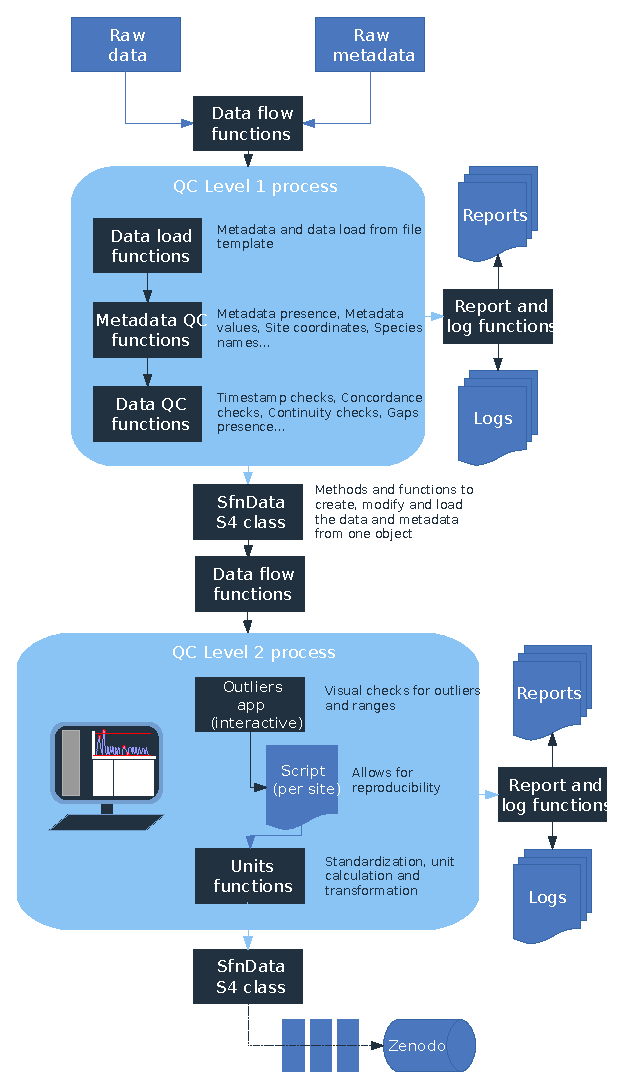
\includegraphics[width=0.7\linewidth]{figure/CH3/Figure1} 

}

\caption[Overview of the SAPFLUXNET data workflow.]{Overview of the SAPFLUXNET data workflow. Data files are received from data contributors, and undergo several quality-control processes (QC1 and QC2). Both, QC1 and QC2 produce an .RData object of the custom-designed sfn-data S4 class storing all data, metadata and data flags for each dataset. The progress and results of the QC processes are monitored through individual reports and log files. The final outcome, is stored in a folder structure with a either single .RData file for each dataset or a set of seven csv files for each dataset.}\label{fig:Ch2plot1}
\end{figure}
\subsection{Data harmonisation and quality control:
QC2}\label{data-harmonisation-and-quality-control-qc2}

Datasets entering QC2 underwent several data cleaning and data
harmonisation processes (Supplement Table S2). We first ran outlier
detection and out of range checks; these checks did not delete or modify
the data, only warned about any suspicious observation (`outlier' and
`range' warnings). The outlier detection algorithm was based on a Hampel
filter, which also estimates a replacement value for a candidate outlier
(Hampel, 1974). For the range checks, we defined minimum and maximum
allowed values for all the time series variables, based on published
values of extreme weather records and maximum transpiration rates
(Cerveny et al., 2007; Manzoni et al., 2013). The outcome of outlier and
range checks were visually inspected on the actual time series being
evaluated using an interactive R Shiny application (Supplement Fig.S3).
Following expert knowledge, visually confirmed outliers were replaced by
the values estimated by the Hampel filter. Similarly, we replaced out of
range values by NA if the variable was out of its physically allowed
range (Supplement Fig.S3). Outlier and out of range `warnings' for each
observation (e.g.~for each variable and timestep) were documented in two
data flags tables, with the same dimensions as the corresponding data
tables (Supplement Fig. S2). Likewise, those observations with confirmed
problematic values, which were removed or replaced, were also flagged;
further information can be found in the `data flags' vignettes in the
`sapfluxnetr' package Granda et al. (Granda et al., 2019)\par

Final data harmonisation processes in QC2 involved unit transformations
and the calculation of derived variables (Supplement Table S2). When
plant sapwood area was provided by data contributors, we interconverted
between sap flow rate per plant and per unit sapwood area. If leaf area
was supplied, we also calculated sap flow per unit leaf area, but note
that this transformation does not take into account the seasonal
variation in leaf area. In QC2 we estimated missing environmental
variables which could be derived from related variables in the dataset
(Appendix, Table A6). We also estimated the apparent solar time and
extraterrestrial global radiation from the provided timestamp and
geographic coordinates using the R package `solaR' (Perpiñán, 2012). All
estimated or interconverted observations were flagged as `CALCULATED' in
the `env\_flags' or `sap\_flags' table (Supplement Fig. S2).\par

\subsection{Data structure}\label{data-structure}

One of the major benefits of the SAPFLUXNET data workflow is the
encapsulation of datasets in self-contained R objects of the S4 class
with a predefined structure. These objects belong to the custom-designed
`sfn\_data' class, which display different slots to store time series of
sap flow and environmental data, their associated data flags, and all
the metadata (Supplement Fig. S2). For further information please see
the `sfn\_data classes' vignette in the `sapfluxnetr' package (Granda et
al., 2019). The code identifying each dataset was created by the
combination of a `country' code, a `site' code and, if applicable, a
`stand' code and a `treatment' code. This means that several `stands'
and/or `treatments' can be present within one `site' (Supplement Table
S3).\par

At the end of the QC process, we generated a folder structure with a
first-level storing datasets as either `sfn\_data' objects or as a set
of comma-separated (csv) text files. Within each of these formats, a
second-level folder groups datasets according to how sap flow is
normalized (per plant, sapwood or leaf area); note that the same
dataset, expressing different sap flow quantities, can be present in
more than one folder (e.g. `plant' and `sapwood'). Finally, the third
level contains the data files for each dataset: either a single
`sfn\_data' object storing all data and metadata, or all the individual
csv files. More details on the data structure can be found in the
`sapfluxnetr-quick-guide' vignette in the `sapfluxnetr' package (Granda
et al., 2019).\par

\section{The SAPFLUXNET database}\label{the-sapfluxnet-database}

\subsection{Data coverage}\label{data-coverage}

The SAPFLUXNET version 0.1.5 database harbours 202 globally distributed
datasets (Fig. 2a, Supplement Fig. S4 and Table S3), from 121
geographical locations, with Europe, Eastern USA and Australia
especially well represented. These datasets were represented in the
bioclimatic space using the terrestrial biomes delimited by Whittaker
(Fig. 2b), but note that, as any bioclimatic classification, it has its
limitations. Datasets have been compiled from all terrestrial biomes,
except for temperate rainforests, although some tropical montane sites
have been included. Woodland/shrubland and temperate forest biomes are
the most represented in the database adding up to 80\% of the datasets
(Fig. 2b). However, large forested areas in the tropics and in boreal
regions are still not well represented (Fig. 2a,b). Looking at the
distribution by vegetation type (Fig. 2c), evergreen needleleaf forest
is the most represented vegetation type (65 datasets), followed by
deciduous broadleaf forest (47 datasets) and evergreen broadleaf forest
(43 datasets).\par

SAPFLUXNET contains sap flow data for 2714 individual plants (1584
angiosperms and 1130 gymnosperms), belonging to 174 species (141
angiosperms and 33 gymnosperms), 95 different genera and 45 different
families (Supplement, Table S4-S5). All species but one, Elaeis
guineensis, a palm, are tree species. Pinus and Quercus are the most
represented genera (Fig. 3b). Amongst the gymnosperms, Pinus sylvestris,
Picea abies and Pinus taeda are the three most represented species with
data provided on 290, 178 and 107 trees, respectively (Fig. 3a). For the
angiosperms, Acer saccharum, Fagus sylvatica and Populus tremuloides are
the most represented species, with 162, 116 and 104 trees, respectively,
although most Acer saccharum data come from a single study with a very
large sample size (Fig. 3a). Some species are present in more than 10
datasets: Pinus sylvestris, Picea abies, Fagus sylvatica, Acer rubrum,
Liriodendron tulipifera and Liquidambar styraciflua (Fig. 3a, Supplement
Table S4).\par

\setlength{\abovecaptionskip}{0pt}
\begin{figure}[H]

{\centering 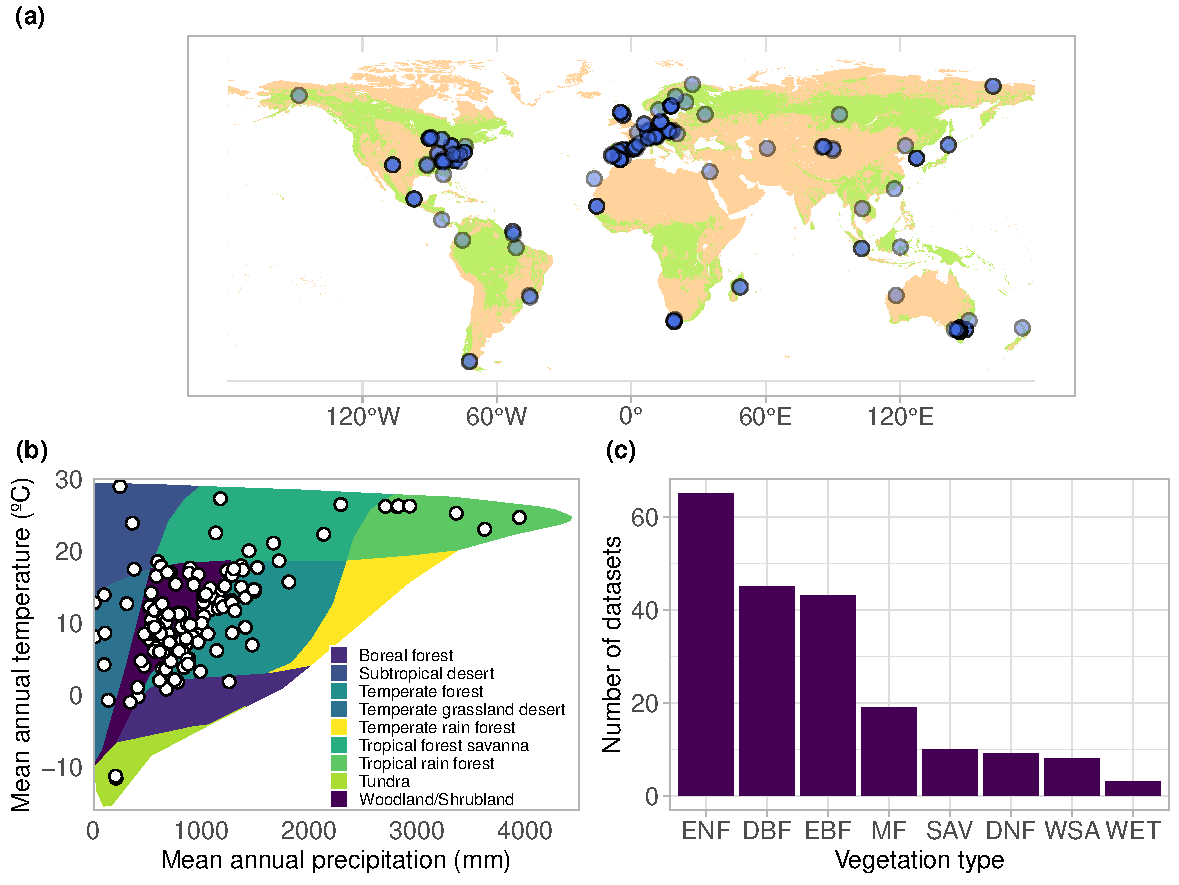
\includegraphics[width=1\linewidth]{figure/CH3/Figure2} 

}

\caption[Geographic, bioclimatic and vegetation type distribution of SAPFLUXNET datasets.]{(a) Geographic, (b) bioclimatic and (c) vegetation type distribution of SAPFLUXNET datasets. In (a) woodland area from Crowther et al. (2015) is shown in green. In (b) we represent the different datasets according to their mean annual temperature and precipitation in a Whittaker diagram showing the classification of the main terrestrial biomes. In (c) vegetation types are defined according to the International Geosphere-Biosphere Programme (IGBP) classification (ENF: Evergreen Needleleaf Forest; DBF: Deciduous Broadleaf Forest; EBF: Evergreen Broadleaf Forest; MF: Mixed Forest; DNF: Deciduous Needleleaf forest; SAV: Savannas; WSA: Woody Savannas; WET: Permanent Wetlands).}\label{fig:Ch2plot2}
\end{figure}
\setlength{\abovecaptionskip}{0pt}
\begin{figure}[H]

{\centering 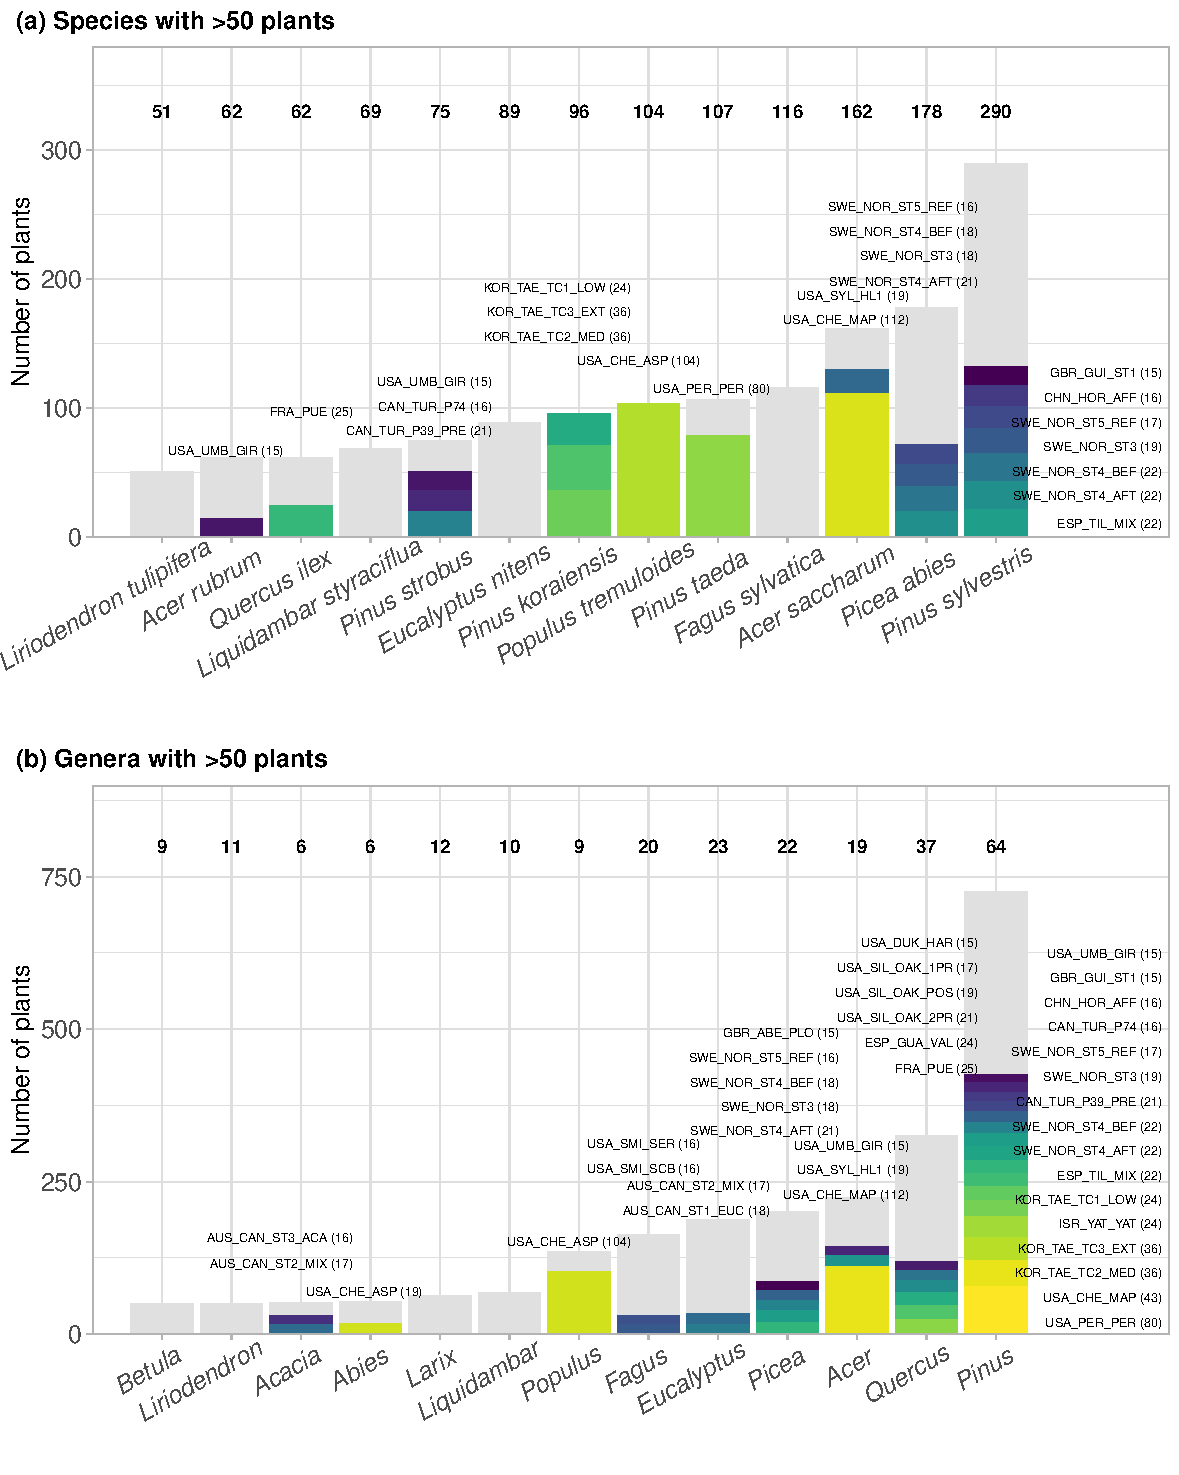
\includegraphics[width=1\linewidth]{figure/CH3/Figure3} 

}

\caption[Taxonomic distribution of genera and species in SAPFLUXNET.]{Taxonomic distribution of genera and species in SAPFLUXNET, showing (a) species and (b) genera with > 50 plants in the database. Total bar height depicts number of plants per species (a) or genera (b). Numbers on top of each bar show the number of datasets where each species (a) or genus (b) is present. Colours other than grey highlight datasets with 15 or more plants of a given species (a) or genus (b). Bar height for a given colour is proportional to the number of plants in the corresponding dataset, which is also shown in parentheses next to the dataset code.}\label{fig:Ch2plot3}
\end{figure}
\subsection{Methodological aspects}\label{methodological-aspects}

For more than 90\% of the plants, sap flow at the whole-plant level is
available (either directly provided by contributors or calculated in the
QC process); this is important for upscaling SAPFLUXNET data to the
stand level (cf.~section 4.2). Because the leaf area of the measured
plants is often not available as metadata, sap flow per unit leaf area
was estimated for only 18.6\% of the individuals (Fig. 4). The heat
dissipation method is the most frequent method in the database (HD,
66.4\% of the plants), followed by the trunk sector heat balance (TSHB,
16.4\%) and the compensation heat pulse method (CHP, 8.4\%) (Fig. 4).
This distribution is broadly similar to the use of each method
documented in the literature, although the TSHB method is
overrepresented here, compared to the current use of this method by the
sap flow community (Flo et al., 2019; Poyatos et al., 2016). Some
methods, especially those belonging to the heat pulse family and the
cyclic (or transient) heat dissipation (CHD) method are mostly used in
angiosperms, while the TSHB and the heat field deformation (HFD) methods
are more frequently used in gymnosperms (Fig. 4).\par

\setlength{\abovecaptionskip}{0pt}
\begin{figure}[hbt!]

{\centering 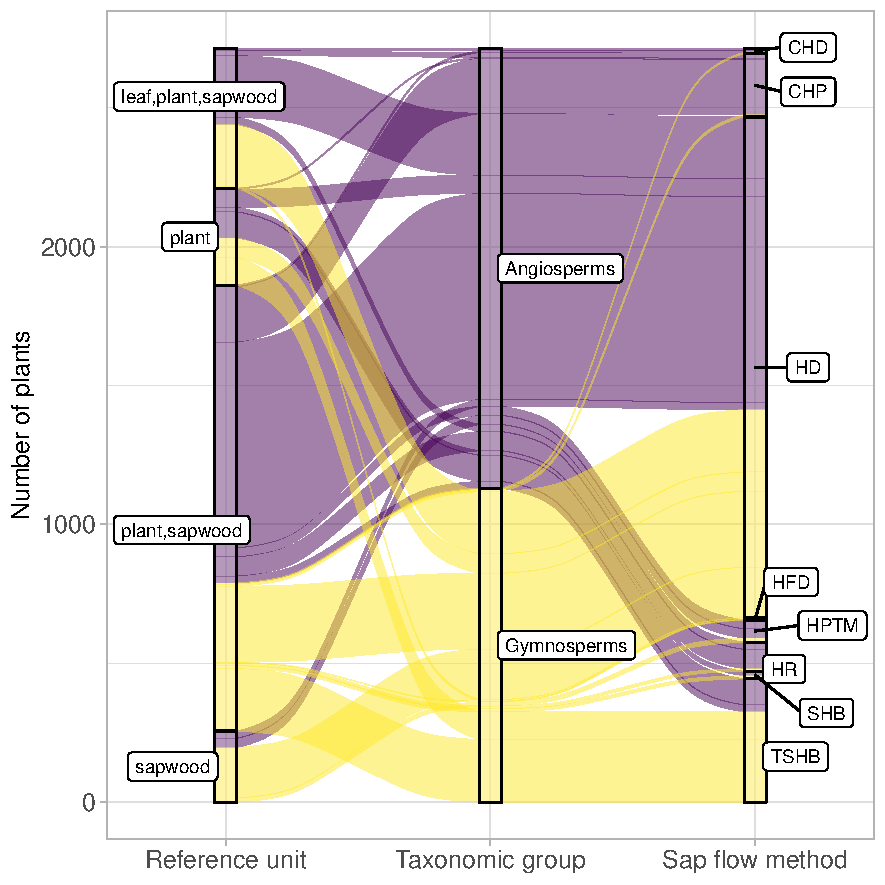
\includegraphics[width=1\linewidth]{figure/CH3/Figure4} 

}

\caption[Distribution of plants according to major taxonomic group and sap flow method.]{Distribution of plants in SAPFLUXNET according to major taxonomic group (angiosperms, gymnosperms), sap flow method (CHD:cycling heat dissipation; CHP: compensation heat pulse; HD: heat dissipation; HFD: heat field deformation: HPTM: heat pulse T-max (HPTM): HRM: heat ratio (HR); SHB: stem heat balance; TSHB: trunk sector heat balance) and reference unit for the expression of sap flow (plant, sapwood area, leaf area). Combinations of reference units imply that data are present in multiple units.}\label{fig:Ch2plot4}
\end{figure}
Calibration of sap flow sensors and scaling from point measurements to
the whole-plant can be critical steps towards accurate estimates of
absolute sap flow rates. In SAPFLUXNET, most of the sap flow time series
have not undergone a species-specific calibration, with the CHD method
showing the highest percentage of calibrated time series (Table 1). This
lack of calibrations may be relevant for the more empirical heat
dissipation methods (HD and CHD), which have been shown to consistently
underestimate sap flow rates (Flo et al., 2019; Peters et al., 2018;
Steppe et al., 2010). Radial integration of single-point sap flow
measurements is more frequent than azimuthal integration (Table 2),
except for the CHD method. A large number of plants using the HD method,
and all plants measured using the HPTM method, do not employ any radial
integration procedure. In contrast, the CHP, HR, SHB, and TSHB methods
are those which more frequently addressed radial variation in one way or
another (Table 2). Azimuthal integration procedures are also more
frequent when the TSHB method is used (Table 2).\par
\begin{table}[!h]

\caption[Number of sap flow times series in SAPFLUXNET depending on whether they were calibrated for the different sap flow methods.]{\label{tab:Ch3T1}Number of sap flow times series in SAPFLUXNET depending on whether they were calibrated (species-specific), non-calibrated or this information was not provided, for the different sap flow methods: cyclic (or transient) heat dissipation (CHD), compensation heat pulse (CHP), heat dissipation (HD), heat field deformation (HFD), heat pulse T-max (HPTM), heat ratio (HR), stem heat balance (SHB) and trunk sector heat balance (TSHB). The percentage of calibrated time series was expressed with respect to the total number of sap flow time series for each method.}
\centering
\fontsize{10}{12}\selectfont
\begin{tabular}[t]{ccccc}
\toprule
Method & Calibrated & Non-calibrated & Not provided & \% calibrated\\
\midrule
CHD & 6 & 13 & 0 & 31.6\\
CHP & 29 & 42 & 157 & 12.7\\
HD & 214 & 1491 & 98 & 11.9\\
HR & 3 & 55 & 47 & 2.9\\
TSHB & 7 & 433 & 4 & 1.6\\
HFD & 0 & 8 & 0 & 0.0\\
HPTM & 0 & 80 & 0 & 0.0\\
SHB & 0 & 27 & 0 & 0.0\\
\bottomrule
\end{tabular}
\end{table}
\begin{table}

\caption[Number of plants in the SAPFLUXNET database using different radial and azimuthal integration.]{\label{tab:Ch3T2}Number of plants in the SAPFLUXNET database using different radial and azimuthal integration approaches for the different sap flow methods: cyclic (or transient) heat dissipation (CHD), compensation heat pulse (CHP), heat dissipation (HD), heat field deformation (HFD), heat pulse T-max (HPTM), heat ratio (HR), stem heat balance (SHB) and trunk sector heat balance (TSHB).}
\centering
\resizebox{\linewidth}{!}{
\fontsize{10}{12}\selectfont
\begin{tabular}[t]{ccc>{\centering\arraybackslash}p{3.5cm}>{\centering\arraybackslash}p{2.5cm}c}
\toprule
\multicolumn{6}{l}{\textbf{Azimuthal integration}} \\
\cmidrule(l{3pt}r{3pt}){1-6}
Method & Measured & Sensor-integrated & Corrected, measured azimuthal variation & No azimuthal correction & Not provided\\
\midrule
CHD & 15 & 0 & 0 & 0 & 4\\
CHP & 61 & 0 & 0 & 167 & 0\\
HD & 216 & 0 & 520 & 1021 & 46\\
HFD & 0 & 0 & 0 & 8 & 0\\
HPTM & 0 & 0 & 0 & 80 & \vphantom{1} 0\\
HR & 7 & 0 & 2 & 88 & 8\\
SHB & 0 & 0 & 0 & 27 & 0\\
TSHB & 0 & 25 & 191 & 219 & 9\\
\addlinespace[0.5em]
\hline
\multicolumn{6}{l}{\textbf{Radial integration}}\\
\hline
\hspace{1em}Method & Measured & Sensor-integrated & Corrected, measured radial variation & No radial correction & Not provided\\
\hline
\hspace{1em}CHD & 0 & 0 & 6 & 13 & 0\\
\hspace{1em}CHP & 222 & 0 & 6 & 0 & 0\\
\hspace{1em}HD & 77 & 3 & 645 & 703 & 142\\
\hspace{1em}HFD & 2 & 0 & 0 & 6 & 0\\
\hspace{1em}HPTM & 0 & 0 & 0 & 80 & 0\\
\hspace{1em}HR & 57 & 1 & 42 & 3 & 2\\
\hspace{1em}SHB & 0 & 27 & 0 & 0 & 0\\
\hspace{1em}TSHB & 0 & 338 & 8 & 89 & 9\\
\bottomrule
\end{tabular}}
\end{table}
\subsection{Plant characteristics}\label{plant-characteristics}

Plant-level metadata is almost complete (99.5\% of the individuals) for
diameter at breast height (DBH), while sapwood area and sapwood depth,
important variables for sap flow upscaling, are not available, or could
not be estimated, for 23\% and 47\% of the plants, respectively. Plant
height and plant age are missing for 42\% and 62\% of the individuals,
respectively. Sap flow data in SAPFLUXNET are representative of a broad
range of plant sizes (Fig. 5a). The distribution of DBH showed a median
of 25.0 cm and 20.4 cm for gymnosperms and angiosperms, respectively,
with a long tail towards the largest plants, two Mortoniodendron
anisophyllum trees from a tropical forest in Costa Rica that measured
\textgreater{} 200 cm (Fig. 5a). The largest gymnosperm tree in
SAPFLUXNET (176 cm in DBH) is a kauri tree (Agathis australis) from New
Zealand. The distribution of plant heights is less skewed, with similar
medians for angiosperms (17.6 m) and gymnosperms (17.5 m). The tallest
plants are located in a tropical forest in Indonesia, where a Pouteria
firma tree reached 44.7 m. Remarkably, of the 16 plants taller than 40
m, over 60\% are Eucalyptus species. The tallest gymnosperm (36.2 m) is
a Pinus strobus from NE USA.\par

\setlength{\abovecaptionskip}{0pt}
\begin{figure}[hbt!]

{\centering 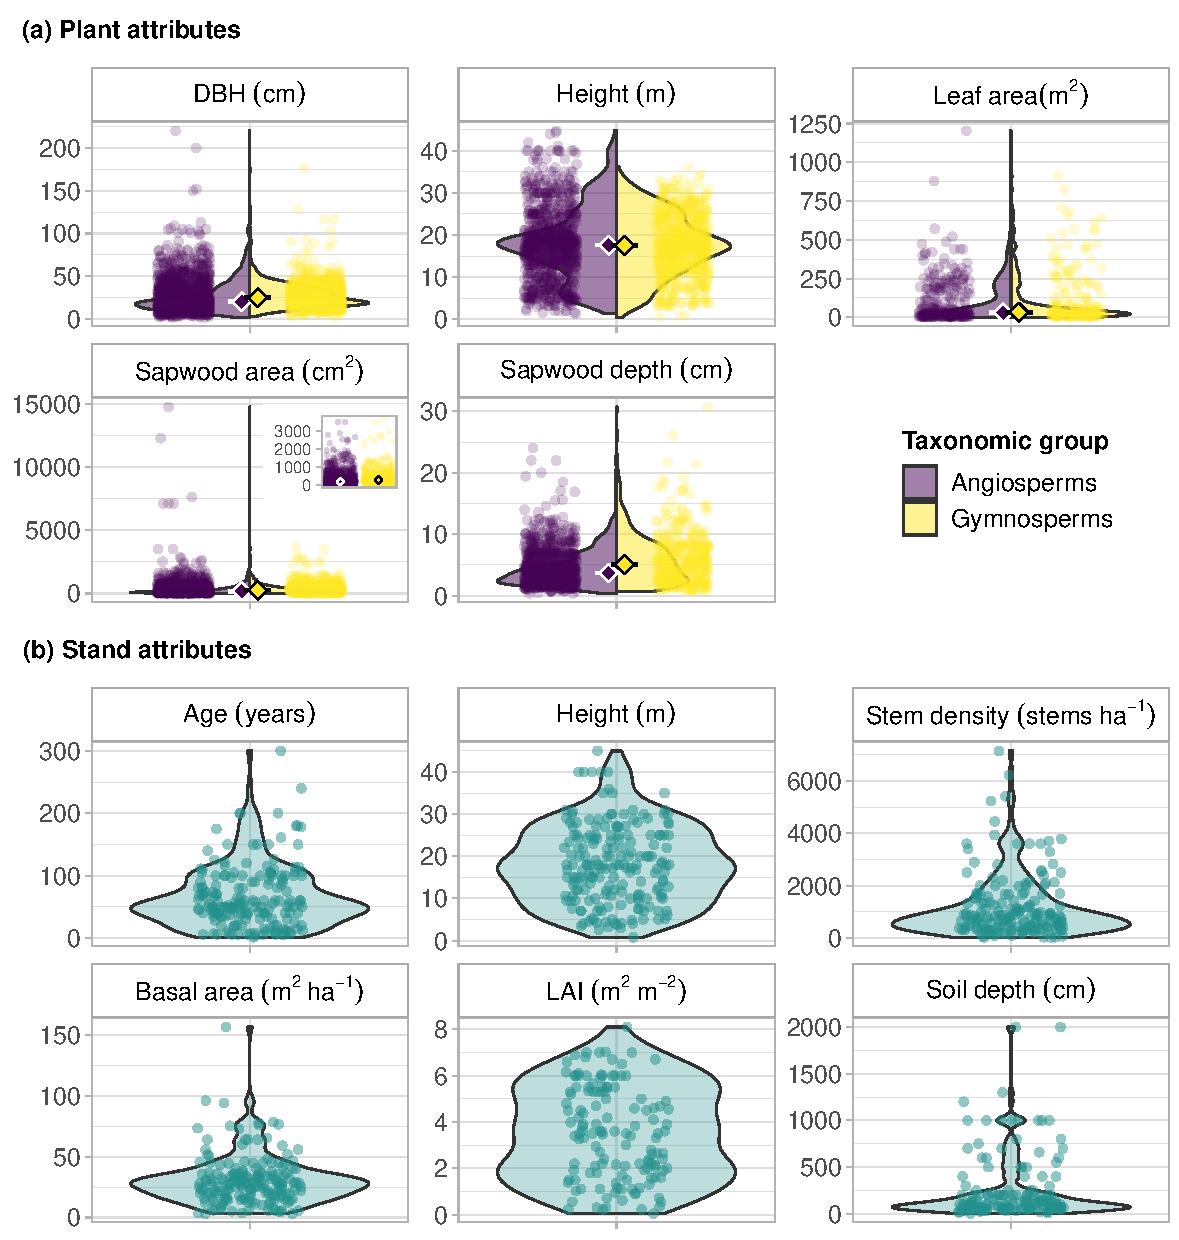
\includegraphics[width=1\linewidth]{figure/CH3/Figure5} 

}

\caption[Characteristics of trees and stands in the SAPFLUXNET database.]{Characteristics of trees and stands in the SAPFLUXNET database. Panel (a) shows plant data and kernel density plots of the main plant attributes, coloured by taxonomic group (angiosperms and gymnosperms): diameter at breast height (DBH), plant height, sapwood area, sapwood depth and leaf area. The inset in the sapwood area panel zooms in values lower than 5000 cm². Panel (b) shows stand data and kernel density plots of the main stand attributes: stand age, stand height, stem density, stand basal area,leaf area index (LAI) and soil depth.}\label{fig:Ch2plot5}
\end{figure}
Plant size metadata in SAPFLUXNET is complemented with plant-level data
of sapwood and leaf area, that provide information on the functional
areas for water transport and loss (Fig. 5a). Distributions of sapwood
and leaf area show highly skewed distributions, with long tails towards
the largest values and slightly higher median values for gymnosperms
(262 cm2 and 33.0 m2 for sapwood and leaf areas, respectively), compared
to angiosperms (168 cm2 and 29.9 m2). Accordingly, median sapwood depth
is also higher for gymnosperms (5.1 cm) compared to angiosperms (3.7
cm). The largest trees (Mortoniodendron, Pouteria, Agathis) with deep
sapwood (17--24 cm) are also those with largest sapwood areas. Many
large angiosperm trees from tropical (CRI\_TAM\_TOW, IDN\_PON\_STE,
GUF\_GUY\_ST2; see Table S3 for dataset codes) and temperate forests
(Fagus grandifolia, USA\_SMIC\_SCB) also show large sapwood areas
(\textgreater{} 5000 cm2), but the plant with the deepest sapwood is a
gymnosperm, an Abies pinsapo in Spain with 30.7 cm of sapwood depth.\par

\subsection{Stand characteristics}\label{stand-characteristics}

Stand-level metadata include several variables associated with
management, vegetation structure and soil properties. Half of the
datasets originate from naturally regenerated, unmanaged stands, and
13.9\% come from naturally regenerated but managed stands. Plantations
add up to 32.2\% and orchards only represent 4\% of the datasets.
Reporting of structural variables is mixed, with stand height, age,
density and basal area showing relatively low missingness (6.4\%,
11.4\%, 12.9\% and 13.4\%, respectively); in contrast, soil depth and
LAI are missing from 26.7\% and 33.7\% of the datasets.\par

SAPFLUXNET datasets originate from stands with diverse structural
characteristics. Median stand age is 54 years and there are several
datasets coming from \textgreater{}100 year-old forests (Fig. 5b). Stand
height shows a similar range and distribution of values compared to
individual plant height (Fig. 5a,b). The denser stands correspond to
coppiced evergreen oak stands from Mediterranean forests (FRA\_PUE,
ESP\_TIL\_OAK), species-rich tropical forests (MDG\_SEM\_TAL) or
relatively young temperate forests (e.g.~FRA\_HES\_HE1\_NON,
USA\_CHE\_MAP). The sparsest stands (\textless{} 200 stems ha-1)
correspond to tree-grass savanna systems (Spain, Portugal, Australia,
Senegal), dry woodlands (China), or oil palm plantations in Indonesia
(IDN\_JAM\_OIL). Stands with the largest basal areas (\textgreater{} 70
m2 ha-1) are mostly dominated by broadleaf species, except for a Picea
abies plantation in Sweden (SWE\_SKO\_MIN).\par

The distribution of leaf area index (LAI) shows a median of 3.5 m2 m-2,
with the largest values observed in temperate (CZE\_BIK, USA\_DUK\_HAR,
HUN\_SIK) and tropical (GUF\_GUY\_GUY, COL\_MAC\_SAF\_RAD) forests. The
stands with the lowest LAI correspond to the sparse woodlands from
Mediterranean and semi-arid locations and also those from forests near
altitudinal or latitudinal tree-lines (FIN\_PET, AUT\_TSC). SAPFLUXNET
datasets show a median soil depth of 100 cm, with only a dozen datasets
originated from sites with soils deeper than 10 m (Fig. 5b).\par

The number of plants per dataset is highly variable, with most of the
datasets (86\%) containing data for at least 4 trees and 46\% of the
datasets having data for at least 10 trees (Fig. 6a, see also Fig. 9).
\par

\setlength{\abovecaptionskip}{0pt}
\begin{figure}[hbt!]

{\centering 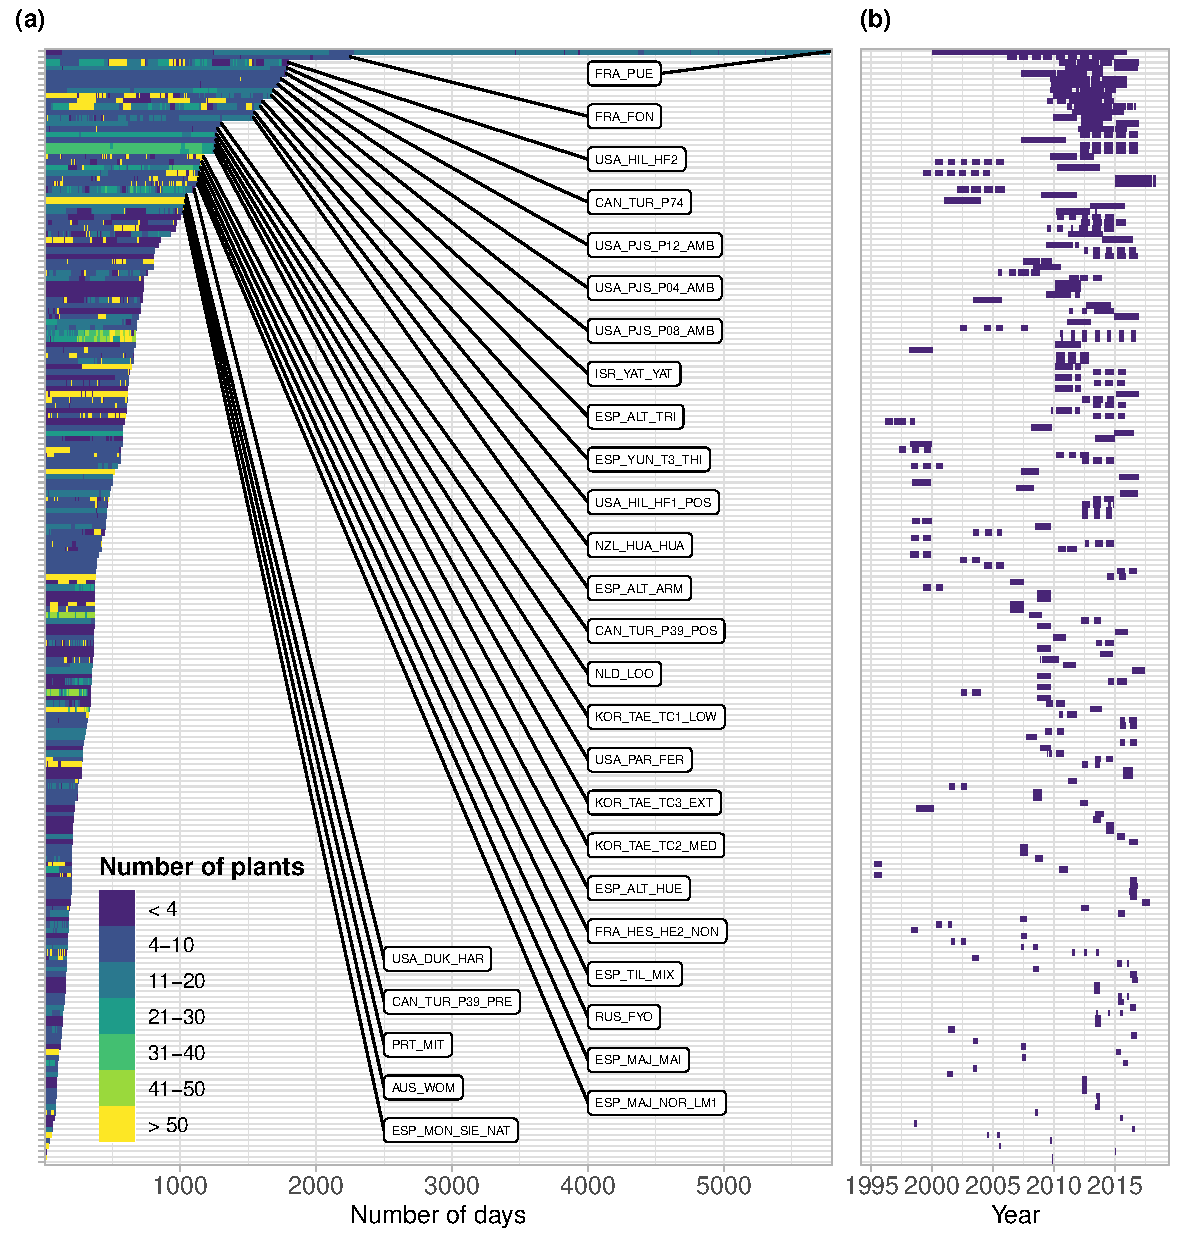
\includegraphics[width=1\linewidth]{figure/CH3/Figure6} 

}

\caption[Duration and number of plants mesured in each dataset.]{(a) Measurement duration of SAPFLUXNET datasets expressed in number of days with sap flow data and coloured by the number of plants measured on each day . The 30 longest datasets are labelled. For each dataset in panel (a), panel (b) shows its corresponding measurement period.}\label{fig:Ch2plot6}
\end{figure}
\subsection{Temporal characteristics}\label{temporal-characteristics}

The oldest datasets in SAPFLUXNET go back to 1995 (GBR\_DEV\_CON,
GBR\_DEV\_DRO) while the most recent data reach up to 2018 (datasets
from the ESP\_MAJ cluster of sites). Several multi-year datasets are
present in SAPFLUXNET (Fig. 6), with 50\% of the datasets spanning a
period of at least 3 years, and some datasets being extraordinarily long
(16 years in FRA\_PUE). Frequently, the datasets only cover the `growing
season' periods, or even shorter periods for some sites which were
eventually included because they improved the ecological and geographic
coverage of the database (e.g.~ARG\_MAZ, ARG\_TRE as representative of
deciduous Nothofagus forest in South Patagonia). In contrast, a few
datasets show continuous records over multiple years (Fig. 6b). Amongst
the longest datasets, most of them come from European or North American
sites (Fig. 6), except some datasets from Israel (ISR\_YAT\_YAT, 7
years), Russia (RUS\_FYO, 7 years), South Korea (KOR\_TAE cluster of
sites, 6 years) or New Zealand (NZL\_HUA\_HUA, 5 years).\par 

SAPFLUXNET provides an unprecedented database to study the detailed
temporal dynamics of plant transpiration across species and sites
globally. Sub-daily records of sap flow (e.g.~at least at hourly
timesteps) are available for extended periods (Fig. 6b), allowing to
address both seasonal and diel patterns in water use regulation by trees
and how these temporal patterns change across species or years across
terrestrial biomes, reflecting different phenologies and water-use
strategies. For instance, in Mediterranean forests, evergreen species
such as Quercus ilex, Arbutus unedo and Pinus halepensis show moderate
sap flow the whole year round, while the deciduous Quercus pubescens
shows higher sap flow density during a shorter period and its water use
is heavily reduced during a dry year (2012) (Fig. 7a). Temperate forests
without water availability limitations show relatively high flows during
the growing season and similar diel sap flow patterns among species
(Fig. 7b). In contrast, tropical forests show moderate to high sap flow
rates during the entire year, with different dynamics in the intradaily
water use regulation across species. For example, Inga sp. in a highly
diverse wet tropical forest in Costa Rica, reduced sap flow during
mid-day hours compared to co-existing species (Fig. 7c).\par

\setlength{\abovecaptionskip}{0pt}
\begin{figure}[hbt!]

{\centering 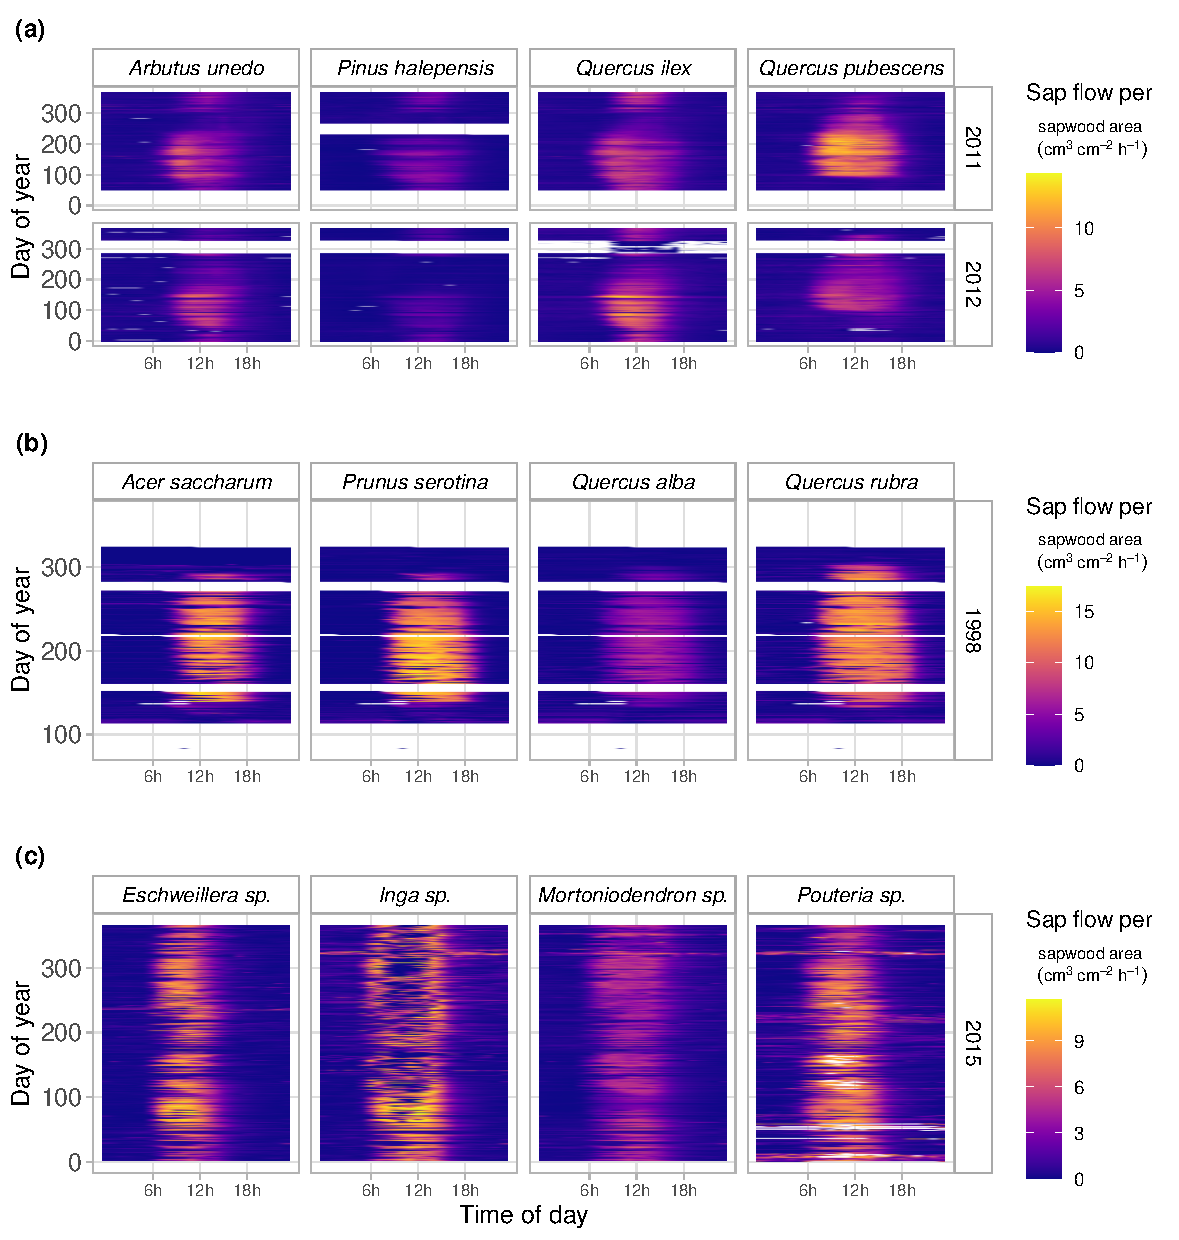
\includegraphics[width=1\linewidth]{figure/CH3/Figure7} 

}

\caption[Fingerprint plots showing hourly sap flow per unit sapwood area.]{Fingerprint plots showing hourly sap flow per unit sapwood area (colour scale) as a function of hour of day (x-axis) and day of year (y-axis) for a selection of SAPFLUXNET sites with at least four co-occurring species. Panel (a) shows data from a Woodland/Shrubland forest in NE Spain (ESP\_CAN), for an average (2011) and a dry (2012) year. Panel (b) shows data for a mesic Temperate forest (USA\_WVF) and panel (c) shows data for a Tropical forest (CRI\_TAM\_TOW). For this latter site, only 4 of the 17 measured species are shown and some of them were only identified at the genus level.}\label{fig:Ch2plot7}
\end{figure}
\subsection{Availability of environmental
data}\label{availability-of-environmental-data}

All SAPFLUXNET datasets contain ancillary time series of the main
hydrometeorological drivers of transpiration, accompanied by information
on where these variables had been measured (Fig. 8a). Air temperature is
available for all datasets. Although vapour pressure deficit (VPD) was
originally absent in 38\% of the datasets (Fig. 8a,b), we could estimate
it for those sites providing air temperature and relative humidity data
(QC Level 2, see section 2.3), and finally only 2 out of the 202
datasets have missing VPD information. For radiation variables,
shortwave radiation was most often provided, compared to
photosynthetically active and net radiation; only 8 out of 202 datasets
do not have any accompanying radiation data. Most of these environmental
variables were measured on-site, with precipitation being the variable
most frequently retrieved from nearby meteorological stations (48\% of
the datasets) (Fig. 8a). Soil water content measured at shallow depth,
typically between 0 and 30 cm below the soil surface, is provided for
56\% of the datasets, while soil moisture from deep soil layers is
available for only 27\% of the datasets.\par

\setlength{\abovecaptionskip}{0pt}
\begin{figure}[hbt!]

{\centering 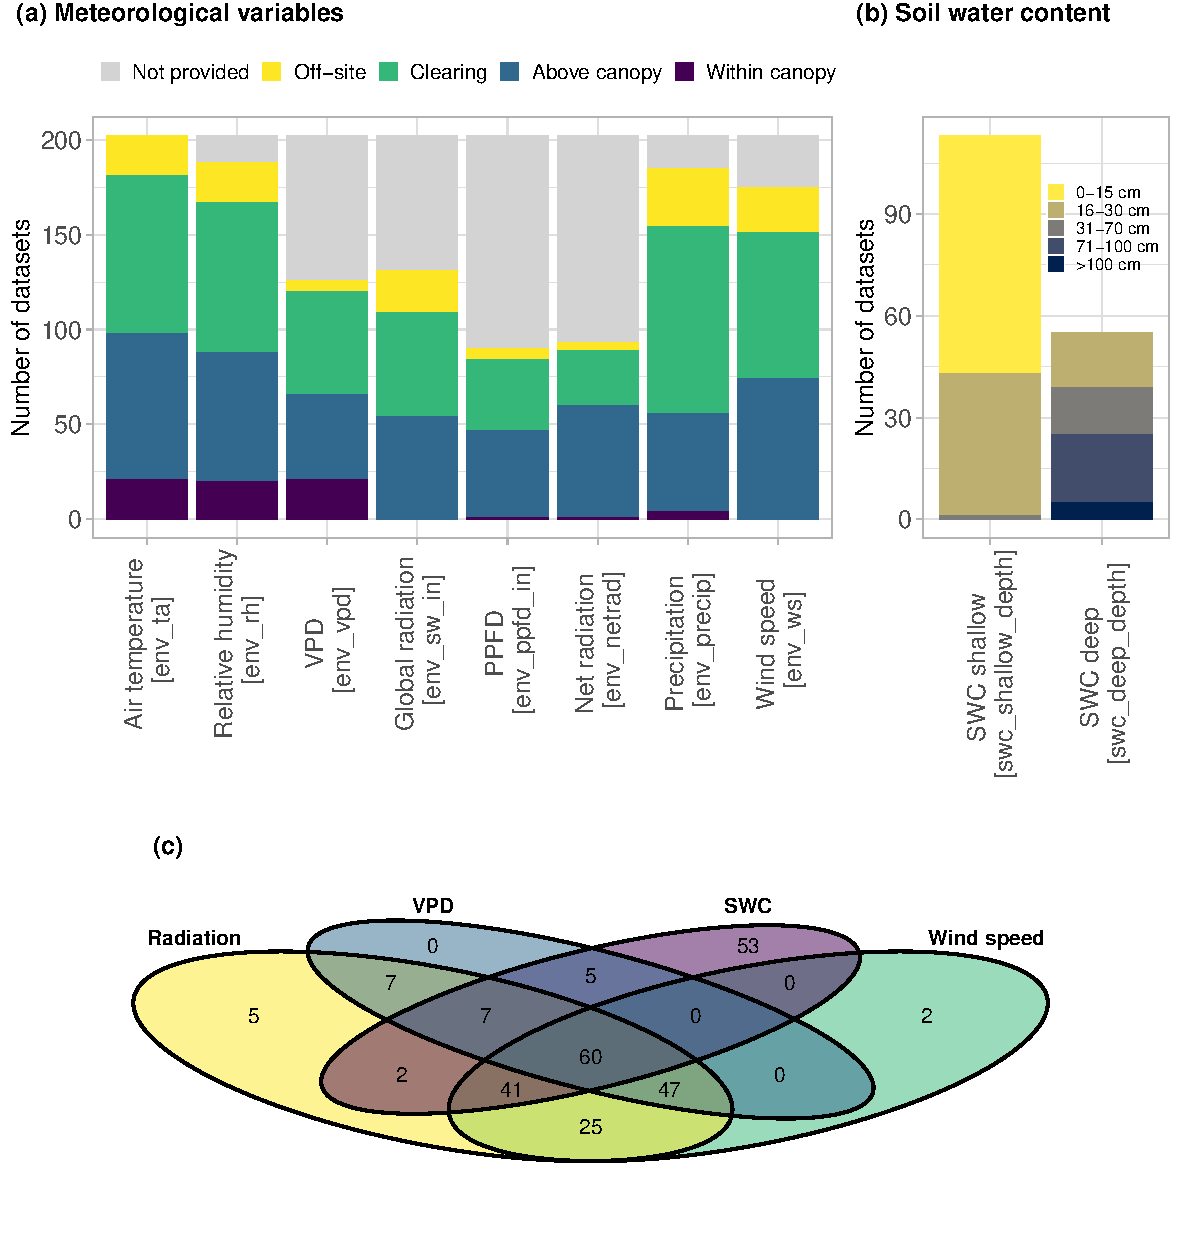
\includegraphics[width=1\linewidth]{figure/CH3/Figure8} 

}

\caption[Summary of the availability of different environmental variables in SAPFLUXNET datasets.]{Summary of the availability of different environmental variables in SAPFLUXNET datasets. (a) Distribution of meteorological variables according to sensor location (in brackets, names of the variables in the database), (b) Distribution of soil moisture variables according to the measurement depth (in brackets, names of the variables in the database). (c) Venn diagram showing the number of datasets where each combination of different environmental variables are present, grouping shortwave, PPFD and net radiation under ‘Radiation’ variables.}\label{fig:Ch2plot8}
\end{figure}
\section{Potential applications}\label{potential-applications}

\subsection{Applications in plant ecophysiology and functional
ecology}\label{applications-in-plant-ecophysiology-and-functional-ecology}

There are multiple potential applications of the SAPFLUXNET database to
assess whole-plant water use rates and their environmental sensitivity,
both across species (e.g.~Oren et al., 1999b) and at the intraspecific
level (Poyatos et al., 2007). SAPFLUXNET will allow disentangling the
roles of evaporative demand and soil water content in controlling
transpiration at the plant level, complementing recent studies looking
at how water supply and demand affect evapotranspiration at the
ecosystem level (Anderegg et al., 2018; Novick et al., 2016). The
availability of global sap flow data at sub-daily time resolution and
spanning entire growing seasons will allow focusing on how maximum water
use and its environmental sensitivity varies with plant-level attributes
such as stem diameter (Dierick and Hölscher, 2009; Meinzer et al.,
2005), tree height (Novick et al., 2009; Schäfer et al., 2000),
hydraulic (Manzoni et al., 2013; Poyatos et al., 2007) and other plant
traits (Grossiord et al., 2019; Kallarackal et al., 2013). SAPFLUXNET
thus provides an unprecedented tool to understand how structural and
physiological traits scale-up to whole-plant regulation of water fluxes
(McCulloh et al., 2019), and how this integration determines drought
responses (Choat et al., 2018) and post-drought recovery patterns (Yin
and Bauerle, 2017). Analyses of the temporal dynamics of plant water use
in response to specific drought events, as recently assessed for gross
primary productivity (e.g.~Schwalm et al., 2017), can also help to
quantify drought legacy effects, including the reversibility of
drought-induced losses of hydraulic conductivity at the plant level.\par

SAPFLUXNET will allow new insights into within-day patterns and controls
in whole-plant water use, which can disclose the fine details of its
physiological regulation. Circadian rhythms can modulate stomatal
responses to the environment, potentially affecting sap flow dynamics
(e.g.~de Dios et al., 2015). Hysteresis in diel sap flow relationships
with evaporative demand and time-lags between evaporative demand and sap
flow, are two linked phenomena likely arising from plant capacitance and
other mechanisms (O'Brien et al., 2004; Schulze et al., 1985), that also
influence diel evapotranspiration dynamics (Matheny et al., 2014; Zhang
et al., 2014). A major driver of time-lags is the use of stored water to
meet the transpiration demand (Phillips et al., 2009), which can now be
analysed across species, plant sizes or drought conditions using time
series analyses, simplified electric analogies (Phillips et al., 1997,
2004; Ward et al., 2013) or detailed water transport models (Bohrer et
al., 2005; Mirfenderesgi et al., 2016). Night-time water use can be
substantial for some species (Forster, 2014; Resco de Dios et al.,
2019). However, available syntheses rely on study-specific
quantification of what constitutes nocturnal sap flow and do not address
possible methodological influences (Zeppel et al., 2014). SAPFLUXNET
will allow applying a consistent estimation of nocturnal sap flow and
control for datasets that are less suitable for the quantification of
night-time fluxes, as information on zero-flow determination is included
in the metadata (`pl\_sens\_cor\_zero', Appendix Table A5).\par

Sap flow data have been widely employed to assess changes in tree water
use after biotic (e.g.~Hultine et al., 2010) or abiotic (Oren et al.,
1999a) disturbances. Likewise, sap flow data have been used to report
changes in species and stand water use following experimental treatments
involving resource availability modifications (e.g.~Ewers et al., 1999)
or density changes (i.e.~thinning, Simonin et al., 2007). The SAPFLUXNET
database includes datasets with experimental manipulations, applied
either at the stand or at the individual level (Table 3). The main
treatments present are related to thinning, water availability changes
(irrigation, throughfall exclusion) and wildfire impact (Table 3),
potentially facilitating new data syntheses and meta-analyses using
these datasets (e.g.~Grossiord et al., 2017).\par
\begin{table}[!h]

\caption[Number of datasets, plants and species by stand-level treatment in the SAPFLUXNET database.]{\label{tab:Ch3T3}Number of datasets, plants and species by stand-level treatment in the SAPFLUXNET database.}
\centering
\fontsize{10}{12}\selectfont
\begin{tabular}[t]{cccc}
\toprule
Treatment & N sites & N plants & N species\\
\midrule
None/control & 155 & 2198 & 170\\
Thinning & 18 & 332 & 18\\
Irrigation & 9 & 36 & 4\\
Post-fire & 6 & 18 & 4\\
CO2 fertilisation & 3 & 28 & 2\\
Drought & 3 & 9 & 2\\
Soil fertilisation & 2 & 16 & 2\\
Post-mortality & 1 & 22 & 5\\
Soil fertilisation and pruning & 1 & 12 & 1\\
Soil fertilisation and thinning & 1 & 12 & 1\\
Pruning and thinning & 1 & 11 & 1\\
Soil fertilisation, pruning and thinning & 1 & 11 & 1\\
Pruning & 1 & 9 & 1\\
\bottomrule
\end{tabular}
\end{table}
The combination of SAPFLUXNET with other ecophysiological databases can
inform on the relative sensitivity of different physiological processes
in response to drought, for example those related to growth and carbon
assimilation (Steppe et al., 2015) . Within-day fluctuations of stem
diameter can be jointly analysed with co-located sap flow measurements
to study the dynamics of stored water use under drought and its
contribution to transpiration (e.g.~Brinkmann et al., 2016), and to
infer parameters on tree hydraulic functioning using mechanistic models
of tree hydrodynamics (Salomón et al., 2017; Steppe et al., 2006;
Zweifel et al., 2007). These analyses could be carried out for a large
number of species by combining SAPFLUXNET with data from the
Dendroglobal database
(\url{http://78.90.202.92/streess/databases/dendroglobal}); there are at
least 18 SAPFLUXNET datasets with dendrometer data in Dendroglobal. This
database and the International Tree-Ring Data Bank (Zhao et al., 2018)
could also be used with SAPFLUXNET to investigate, at the species level,
the link between radial growth and water use, including their
environmental sensitivity (Morán-López et al., 2014), and how these two
processes comparatively respond to drought (Sánchez-Costa et al., 2015).
Moreover, given the tight link between water use and carbon
assimilation, combining SAPFLUXNET with water-use efficiency from plant
\textbackslash{}delta13C data could potentially be used to estimate
whole-plant carbon assimilation (Hu et al., 2010; Klein et al., 2016;
Rascher et al., 2010; Vernay et al., 2020), a quantity that is difficult
to measure directly, especially in field-grown, mature trees.\par

The two first PCA axes explained 60\% of the variability of the 12
climatic variables (Appendix B Figure B.2). The niche of \emph{P.
halepensis} characterized with inter-annual variability (inter-annual
variability-based niche) was 42\% larger than the niche estimated with
the average dataset (average-based niche). These differences implied
that during the extreme climatic year, 93.3\% of unaffected forests and
63.3\% of highly affected forests were inside the \emph{P. halepensis}
niche estimated with inter-annual variability. These values diminished
to 52.8\% for unaffected forests and 21.2\% for highly affected ones
when niche was calculated with average climate (Figure 3.2).\par

\subsection{Applications in ecosystem ecology and
ecohydrology}\label{applications-in-ecosystem-ecology-and-ecohydrology}

SAPFLUXNET will provide a global look at plant water flows to bridge the
scales between plant traits and ecosystem fluxes and properties
(Reichstein et al., 2014). Vegetation structure, species composition and
differential water use strategies among and within species scale-up to
different seasonal patterns of ecosystem transpiration, with a strong
influence on ecosystem evapotranspiration and its partitioning. Global
controls on evaporative fluxes from vegetation have been mostly
addressed using ecosystem (Williams et al., 2012) or catchment
evapotranspiration data (Peel et al., 2010). These studies have
described global patterns in evapotranspiration driven by different
plant functional types or climates, but they cannot be used to quantify
and to explain the enormous variation in the regulation of transpiration
across and within taxa.\par

The SAPFLUXNET database will provide a long-demanded data source to be
used in ecohydrological research (Asbjornsen et al., 2011). Upscaling
individual measurements to the stand level (Čermák et al., 2004; Granier
et al., 1996; Köstner et al., 1998) is necessary to quantitatively
compare sap-flow based transpiration with evapotranspiration and
transpiration estimates at the ecosystem scale and beyond. Even though
SAPFLUXNET was designed to accommodate sap flow data at the plant level,
scaling to the ecosystem level is possible for many datasets. For a
basic upscaling exercise using SAPFLUXNET data (Poyatos et al., 2020b),
whole-plant sap flow can be normalised by individual basal area (as DBH
is usually available in the metadata, cf.~section 3.3), averaged for a
given species and then scaled to stand level transpiration using total
stand basal area and the fraction of basal area occupied by each
measured species (see stand metadata, Table A3). For many datasets, sap
flow data are available for the species comprising most of the stand
basal area (often even 100\%, Fig. 9), but species-based upscaling may
be unfeasible in many tropical sites (Fig. 9b), where size-based scaling
could be applied instead (e.g.~da Costa et al., 2018). Further
refinements of the upscaling procedure could be achieved by using trunk
diameter distributions of the sap flow plots (Berry et al., 2018). This
information, however, is not readily available in SAPFLUXNET, and other
data sources (e.g.~forest inventories, LIDAR data) or additional
simplifying assumptions (i.e.~applying the size distribution of measured
individuals in the dataset) would be needed.\par

\setlength{\abovecaptionskip}{0pt}
\begin{figure}[H]

{\centering 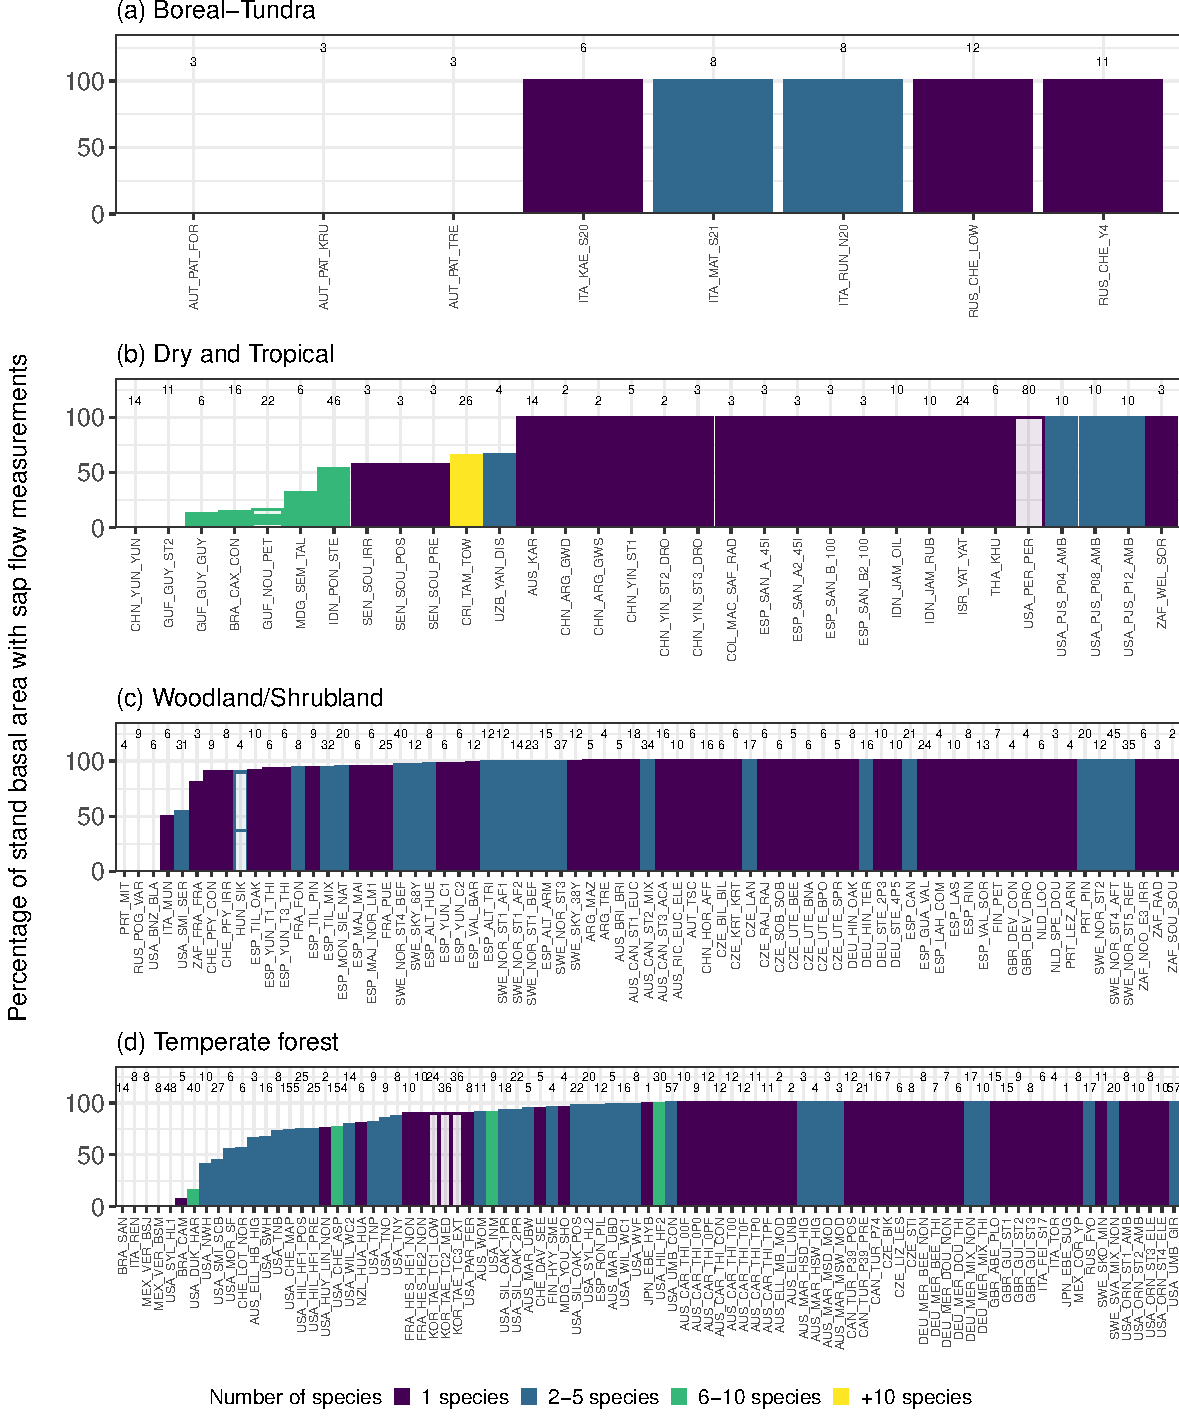
\includegraphics[width=1\linewidth]{figure/CH3/Figure9} 

}

\caption[Potential for upscaling species-specific plant sap flow to stand-level.]{Potential for upscaling species-specific plant sap flow to stand-level sap flow using SAPFLUXNET datasets. Datasets are shown using an aggregated biome classification; ‘Dry and Tropical’ include: ‘Subtropical desert’, ‘Temperate grassland desert’,‘Tropical forest savanna’ and ‘Tropical rain forest’. Each panel shows the percentage of total stand basal area that is covered by sap flow measurements for each species in the dataset. Datasets are also coloured by the number of species present. Numbers on top of each bar depict the total number of plants for a given dataset. Empty bars show datasets for which sap flow data expressed at the plant level were not available.}\label{fig:Ch2plot9}
\end{figure}
Stand-level transpiration estimates from a large number of SAPFLUXNET
sites can contribute to improve our understanding of the role of forest
transpiration in the context of stand water balance and its components
at the ecosystem (e.g.~Tor-ngern et al., 2018) and catchment levels
(Oishi et al., 2010; Wilson et al., 2001). Importantly, SAPFLUXNET can
contribute to better understand the global controls on vegetation water
use (Good et al., 2017), including the biological and climatic controls
on evapotranspiration partitioning into transpiration and evaporation
components (Schlesinger and Jasechko, 2014; Stoy et al., 2019). There is
some overlap between the FLUXNET network and SAPFLUXNET (47 datasets
from FLUXNET sites). Hence, transpiration from SAPFLUXNET can also be
used as a `ground-truth' reference for transpiration estimates from
remote sensing approaches (Talsma et al., 2018) and from eddy covariance
data (Nelson et al., accepted). Extrapolating sap flow-derived stand
transpiration to large spatial scales can be challenging due to
landscape-scale variation in forest structure (Ford et al., 2007) or
topography (Hassler et al., 2018), and to the low spatial
representativeness of sap flow measurements (Mackay et al., 2010). A
promising research avenue to help elucidate the role of vegetation in
driving hydrological changes across environmental gradients (Vose et
al., 2016) would be to combine species-specific stand transpiration data
from SAPFLUXNET with stand structural and compositional data from forest
inventories (e.g.~sapwood area index, Benyon et al., 2015).\par

Understanding the patterns and mechanisms underlying species
interactions with respect to water use within a community is necessary
to predict tree species vulnerability to drought (Grossiord, 2019).
Multispecies datasets from SAPFLUXNET (Table S4) can be used to assess
competition for water resources among species, for example by
identifying changes in seasonal water use across co-existing species and
hence characterizing the spatiotemporal segregation of their
hydrological niches (Silvertown et al., 2015). By providing a detailed
seasonal quantification of tree water use, SAPFLUXNET could also
complement isotope-based studies and contribute to interpret the large
diversity in root water uptake patterns observed worldwide (Barbeta and
Peñuelas, 2017; Evaristo and McDonnell, 2017) and to explain the
different seasonal origin of root-absorbed water across species and
environmental gradients (Allen et al., 2019).\par

Plant water fluxes and hydrodynamics are amongst the most uncertain
components of ecosystem and terrestrial biosphere models (Fatichi et
al., 2016; Fisher et al., 2018). These models are now incorporating
hydraulic traits and processes in their transpiration regulation
algorithms (Mencuccini et al., 2019), but multi-site assessments of
these algorithms are usually performed against evapotranspiration from
eddy flux data (Knauer et al., 2015; Matheny et al., 2014). Model
validation against sap flow data has been carried out typically in only
one (Kennedy et al., 2019; Williams et al., 2001) or few (Buckley et
al., 2012) sites. SAPFLUXNET can thus contribute to assess the
performance of models simulating transpiration of stands or species
within stands (e.g.~De Cáceres et al., submitted.), for a large number
of species and under diverse climatic conditions.\par

\section{Limitations and future
developments}\label{limitations-and-future-developments}

\subsection{Limitations}\label{limitations}

Sap flow data processing differs within and among methods, because
different algorithms, calibrations or parameters involved in sap flow
calculations may be applied. All of these methods contribute to
methodological uncertainty (Looker et al., 2016; Peters et al., 2018)
and this challenging methodological variability precludes the
implementation of a complete, standardised data workflow from raw to
processed data within SAPFLUXNET, as it is done for eddy flux data
(Vitale et al., 2020; Wutzler et al., 2018). Commercial software for sap
flow data processing from multiple methods is available
(i.e.~\url{http://www.sapflowtool.com/SapFlowToolSensors.html}) but it
has not yet been widely adopted. Freely available data-processing
software is only available for the HD method (Oishi et al., 2016;
Speckman et al., 2020; Ward et al., 2017).\par

Sap flow measured with thermometric methods provides a precise estimate
of the temporal dynamics of water flow through plants (Flo et al.,
2019). However, their performance in measuring absolute flows is mixed.
While some well-represented methods in SAPFLUXNET such as the CHP yield
accurate estimates (at least for moderate-to-high flows), the HD method,
the most represented method by far, can significantly underestimate
water flows (Flo et al., 2019). Because plant-level metadata contain
information that document the conversion from raw to processed data
(Appendix Table A5), a first-order correction for uncalibrated HD
measurements based on available methodological assessments can be
applied to allow intercomparability across methods. Nevertheless, given
the high unexplained variability (i.e.~by species and wood traits) in
the performance of sap flow calibrations (Flo et al., 2019), these
corrections should be applied with caution. The determination of zero
flow conditions (baselining) can also have significant impacts on the
quantification of absolute flow for several methods (Peters et al.,
2018; Smith and Allen, 1996; Steppe et al., 2010). The different
baselining approaches are also documented in the metadata to inform data
syntheses and/or to selectively apply correction factors.\par

SAPFLUXNET has been designed to store whole-plant sap flow data, and
therefore, sap flow measured at multiple points within an individual is
not available in the database. Even though this spatial variation could
be useful to describe detailed aspects of plant water transport
(Nadezhdina et al., 2009), focusing on plant-level data greatly
simplifies the data structure. Hence, SAPFLUXNET only includes data
already upscaled to the plant level by the data contributors. The main
details of how this upscaling process was done for each dataset are
provided together with other plant metadata (Table A5), but these
metadata show that within-plant variation in sap flow is often not
considered (Table 2). The impact of not accounting for radial and
circumferential variability when scaling single-point measurements of
sap flow to the whole-plant level can be important (Merlin et al.,
2020), but the estimation of sapwood area can also cause large errors
(Looker et al., 2016). SAPFLUXNET does not provide information on the
method employed to quantify sapwood area (e.g.~visual estimation with or
without the application of dyes, indirect estimation through allometries
at species or site levels) or on the accuracy of sapwood area data. This
precludes uncertainty estimation at the individual level. Future
developments in the SAPFLUXNET data structure could include this
information as metadata to better document the sensor-to-plant scaling
process.\par

While SAPFLUXNET makes global sap flow data available for the first
time, we note that spatial coverage is still sparse and some forested
regions are underrepresented in the database (Fig. 2a). We note
especially the relatively small number of datasets for boreal and
tropical forests, two important biomes in terms of global water and
carbon fluxes (Beer et al., 2010; Schlesinger and Jasechko, 2014). While
many geographic gaps are caused by the absence of sap flow studies from
such areas, some regions where sap flow studies have been conducted are
still not represented in SAPFLUXNET. For example, the recent
proliferation of Asian sap flow studies (Peters et al., 2018) has not
translated into a high representativity of Asian datasets in SAPFLUXNET
yet. Similarly, while the coverage of taxonomic and biometric diversity
is unprecedented, SAPFLUXNET lacks data for the extremely tall trees
(Ambrose et al., 2010) or for other growth forms such as shrubs (Liu et
al., 2011), lianas (Chen et al., 2015) and other non-woody species (Lu
et al., 2002).\par

\subsection{Outlook}\label{outlook}

The public release of SAPFLUXNET has set the stage for a first
generation of sap flow-based data syntheses. The work on these syntheses
will fuel new ideas and tools for future improvements of the database,
as for example new computing approaches for the processing and analysis
of sap flow datasets. One example would be the development of robust
imputation algorithms to gap-fill time series of sap flow and
environmental data, which can take advantage of tools and datasets
already developed by the ecosystem flux community (Moffat et al., 2007;
Vuichard and Papale, 2015). The dissemination of SAPFLUXNET will
encourage the use of machine-learning algorithms, only occasionally used
to analyse sap flow datasets so far (e.g.~Whitley et al., 2013). These
approaches can also be used to identify the relative importance of
different hydrometeorological drivers of transpiration (Zhao et al.,
2019), or to produce global transpiration maps, by combining SAPFLUXNET
with other data (Jung et al., 2019). This upscaling of stand
transpiration to large areas will also allow addressing broader
questions at the regional and continental scale, such as the role of
transpiration in moisture recycling (Staal et al., 2018).\par

The eventual success of this initiative, in terms of enabling data
reuse, contributing towards the understanding and modelling of tree
water use at local to global scales will likely encourage the sap flow
community to contribute new datasets to future updates of the database.
We expect that the development of open-source software for the
processing of sap flow raw data (Speckman et al., 2020), its eventual
widespread use by the sap flow community and the adoption of
standardized calibration practices will increase the quality and
intercomparability of future sap flow datasets. These new datasets will
hopefully expand the temporal, geographical and ecological
representativity of SAPFLUXNET when new data contribution periods can be
opened in the future.\par

\section{Data availability, access and
feedback}\label{data-availability-access-and-feedback}

In this paper we present SAPFLUXNET version 0.1.5 (Poyatos et al.,
2020a), which contains some small metadata improvements on version
0.1.4, the first one to be made publicly available, in March 2020. Both
versions supersede version 0.1.3 which was initially released to data
contributors in March 2019. The entire database can be downloaded from
its hosting webpage in the Zenodo repository
(\url{https://doi.org/10.5281/zenodo.3971689}, Poyatos et al. 2020a). In
this repository, we provide the database as separate .csv files and as
.RData objects; see section 2.4. for details on data structure. Together
with the initial publication of SAPFLUXNET in March 2019, we also
released the sapfluxnetr R package, available on CRAN, to enable easy
access, selection, temporal aggregation and visualisation of SAPFLUXNET
data. Feedback on data quality issues can be forwarded to the SAPFLUXNET
initiative email address:
\href{mailto:sapfluxnet@creaf.uab.cat}{\nolinkurl{sapfluxnet@creaf.uab.cat}}.
All the information about SAPFLUXNET, including the publication of new
calls for data contribution, can be found in the project website:
\url{http://sapfluxnet.creaf.cat/./par}

\section{Conclusion}\label{conclusion}

The SAPFLUXNET database provides the first global perspective of water
use by individual plants at multiple timescales, with important
applications in multiple fields, ranging from plant ecophysiology to
Earth-system science. This database has been built from
community-contributed datasets and is complemented with a software
package to facilitate data access. Both the database and the software
have been implemented following open science practices, ensuring public
access and reproducibility. Data sharing has been a key component of the
success of the FLUXNET network of ecosystem fluxes (Bond‐Lamberty,
2018), and many databases in plant and ecosystem ecology now offer open
data (Bond-Lamberty and Thomson, 2010; Falster et al., 2015; Gallagher
et al., 2020; Kattge et al., 2020). SAPFLUXNET fully aligns with this
philosophy. We expect that this initial data infrastructure will promote
data sharing among the sap flow community in the future (Dai et al.,
2018) and will allow the continued growth of the SAPFLUXNET database.

\chapter[Climate and functional traits jointly mediate tree water use strategies]{Climate and functional traits jointly mediate tree water use strategies}

\setlength{\parindent}{0pt} Victor Flo, Jordi Martínez-Vilalta, Maurizio
Mencuccini1,3, Victor Granda, William R. L. Anderegg, Rafael Poyatos

\newpage

\setlength{\parindent}{30pt}

\section*{Abstract}

Tree water use is central to plant function and ecosystem fluxes.
However, it is still unknown how organ-level water relations traits are
coordinated to determine whole-tree water use strategies in response to
drought, and if this coordination depends on climate. Here we used a
global sap flow data base (SAPFLUXNET) to study the response of water
use, in terms of whole-tree canopy conductance (\(G\)), to vapour
pressure deficit (VPD) and to soil water content (SWC) for 142 tree
species. We investigated the individual and coordinated effect of six
water relations traits (vulnerability to embolism, Huber value,
hydraulic conductivity, turgor-loss point, rooting depth and leaf size)
on water use parameters, also accounting for the effect of tree height
and climate (mean annual precipitation, MAP). Reference \(G\) and its
sensitivity to VPD were tightly coordinated with water relations traits
rather than with MAP. Species with efficient xylem transport had higher
canopy conductance but also higher sensitivity to VPD. Moreover, we
found that angiosperms had higher reference \(G\) and higher sensitivity
to VPD than gymnosperms. Our results highlight the importance of trait
coordination and the complications of defining a single, whole-plant
resource use spectrum ranging from `acquisitive' to `conservative'.\par
\newpage

\section{Introduction}\label{introduction}

Plant water use is a key component of the global water cycle (Katul et
al., 2012). Plants regulate water use across a broad range of timescales
to maintain a favourable water status under varying water availability
(Feng et al., 2017). This regulation is the result of evolutionary
processes together with environmental and biophysical constraints that
have determined a huge diversity of species-specific water use
strategies mediated by a particular suite of traits (Bacelar et al.,
2012; Lu et al., 2020). These specific strategies determine plant
survival under drought (Mitchell et al., 2013), species coexistence
(Ehleringer et al., 1991; Jackson et al., 1995) and ecosystem CO2 and
water fluxes (Mencuccini et al., 2019a). Thus, a comprehensive
understanding of how regulation of whole-plant water use relates to
organ-level water relations traits would allow for a better
characterization of plant responses to drought and improved prediction
of climate change impacts on vegetation (Anderegg, 2015).\par

Among many other traits, the sensitivity of stomata to drought stress is
a major regulator of plant water use over relatively short timescales
(Martin-StPaul et al., 2017). In the absence of effective stomatal
control under drought, water uptake by roots might not compensate water
loss, resulting in high tensions in plants' vascular system, which can
trigger the entrance of air bubbles leading to xylem embolism (Tyree \&
Zimmermann, 2002). If embolism spreads to most of the xylem conduits,
water transport becomes restricted and plants may eventually die from
hydraulic failure (Tyree \& Sperry, 1988; Choat et al., 2018). Through
stomatal closure, plants reduce whole-plant canopy conductance (\(G\))
and therefore water loss and embolism risk, and maintain water status
within tolerable limits, at the expense, however, of reducing gas
exchange. Plants close stomata in response to drops in leaf and/or soil
water potentials (see Martínez-Vilalta \& Garcia-Forner, 2017) produced
by increased atmospheric water demand (i.e., vapor pressure deficit;
VPD) and reduced soil water availability (i.e., soil water content; SWC)
(Jarvis, 1976; Grossiord et al., 2017). Stomatal responses have been
largely described using semi-empirical models (Jarvis, 1976; Oren et
al., 1999; Damour et al., 2010) and optimality approaches relying on the
coupling of photosynthesis and transpiration (Wang et al., 2020), with a
recent focus on plant hydraulics (Sperry et al., 2016). Global syntheses
of these two approaches exist (Lin et al., 2015; Hoshika et al., 2018)
but they are only at the leaf level, and they do not consider the
coordination of stomatal and hydraulic traits.\par 

Coordination among stomatal sensitivity and other hydraulic and
allocation traits is thought to underlie differences in water use
strategies among species (Meinzer, 2002; Sperry et al., 2016; McCulloh
et al., 2019). Because in woody plants water has to be transported from
the soil through the xylem to supply leaf transpiration, the hydraulic
properties of the xylem are key determinants of plant water relations
and water use strategies. Particularly, maximum sapwood hydraulic
conductivity (\(K_s\); Table 1) and vulnerability to xylem embolism
(usually quantified as \(\Psi_{P50}\); i.e.~the water potential at which
half of \(K_s\) is lost) are key determinants of maximum transpiration
rates (Manzoni et al., 2013). In addition, a vulnerable xylem (i.e.~high
\textbar{}\(\Psi_{P50}\)\textbar{}) has been related to higher
canopy-level stomatal sensitivity to VPD across (Litvak et al., 2012)
and within some species (Aspinwall et al., 2011). \(K_s\) and
\(\Psi_{P50}\) have been hypothesized to define a safety-efficiency
trade-off at the tissue level, by which species with high \(K_s\) (i.e.,
high water transport efficiency) are also more vulnerable to embolism
(low \textbar{}\(\Psi_{P50}\)\textbar{} and low safety) and vice versa
(Venturas et al., 2017). However, this trade-off appears to be weak at
the global scale across species, at least as captured with current
measurement techniques (Gleason et al., 2016; Sanchez‐Martinez et al.,
2020). At the leaf level, another key component is the water potential
at turgor-loss point (\(\Psi_{TLP}\)), which is tightly associated with
drought tolerance and habitat water availability (Bartlett et al.,
2012). \(\Psi_{TLP}\) is also closely related to water potential at
complete stomatal closure (Brodribb \& Holbrook, 2003; Martin-StPaul et
al., 2017), and thus can be used as a proxy for quantifying the
sensitivity of plant water use to changes in water availability.\par

Allocation ratios between the organs involved in water loss, transport
and uptake are also important determinants of water use strategies. The
ratio of cross-sectional sapwood area to leaf area or Huber value
(\(Hv\)) is a major trait defining water use strategies because it
expresses the water conducting area per unit transpiring area. Increased
\(Hv\) can contribute to reduce water potential gradients within the
plant and therefore potentially compensate for a species vulnerable
xylem (Mencuccini et al., 2019b). In addition, a high \(Hv\) has also
been associated to strict stomatal control in conifers (Martínez-Vilalta
et al., 2004; Poyatos et al., 2007) and to higher reference canopy
conductance (Novick et al., 2009). Similarly, increasing rooting depth
(\(R_{depth}\)) gives access to deeper water sources, which potentially
allows maintaining less negative and stable water potentials as well as
supporting high water use even under climates with high evaporative
demand (Martínez-Vilalta \& Garcia-Forner, 2017). At the leaf level, the
importance of individual leaf size (\(L_s\)) for light penetration and
crown architecture has been thoroughly studied (Sellers, 1985), but its
influence on water use strategies has been little explored, despite the
role of leaf evaporative cooling for thermoregulation (Wright et al.,
2017). Large leaves with thick leaf boundary layers and an ineffective
stomatal control of water loss (Jarvis \& McNaughton, 1986), may need to
sustain higher transpiration rates to maintain leaf temperature within
operative limits under intense radiative heating and/or heat waves
(e.g.~Drake et al., 2018). This may lead to a trade-off between leaf
thermoregulation and the conservation of water and/or hydraulic function
(Fauset et al., 2018), especially in hotter sites (Aparecido et al.,
2020).\par

Water use strategies are also mediated by plant height, community
composition, and environmental conditions, particularly climate,
topography and soil properties; as well as spatial and temporal
variability in environmental conditions (Feng et al., 2018). Plant
height increases hydraulic path length and hydraulic resistance, and
thus plays a major role in the global coordination of several water use
traits such as \(\Psi_{P50}\) or \(K_s\) (Liu et al., 2019), \(Hv\)
(Mencuccini et al., 2019b) and reference canopy conductance (Novick et
al., 2009). Likewise, increasing tree height has been related to
enhanced sensitivity of canopy conductance to VPD for some species
(Schäfer et al., 2000). Because soil water is a common resource
belowground that is influenced by water uptake from many individuals and
species, the community composition and diversity of water use strategies
in an ecological community can also affect ecosystem fluxes and drought
progression (Anderegg et al., 2018, 2019). In addition, phylogeny may
constrain flexibility in water use strategies independently of the
environment, as it has been shown for example by the consistent
differences in hydraulic traits between angiosperms and gymnosperms
(Johnson et al., 2012; Bartlett et al., 2016) and by the strong
phylogenetic conservatism reported for some hydraulic traits such as
\(\Psi_{P50}\) and \(K_s\) at the global scale (Sanchez‐Martinez et al.,
2020).\par

In this study we explore water use strategies across tree species using
a trait-based approach, which provides a simplified framework to
understand species responses to drought at the global scale (Feng et
al., 2018). Our ultimate aim is to better understand how water use
strategies emerge from the covariation between traits and the influence
of climate. To that end, we use a global database of sap flow
measurements (SAPFLUXNET) to calculate whole-tree canopy conductance
(\(G\)) for 142 tree species growing on 126 sites. We then parameterize
the response of G to VPD and SWC at the species level and for major
taxonomic groups (i.e.~angiosperms and gymnosperms). Finally, we
characterize the relationships between water use traits and key
hydraulic and allocation traits among species (i.e. \(\Psi_{P50}\),
\(K_s\), \(Hv\), \(\Psi_{TLP}\), \(R_{depth}\), \(L_s\) and tree
height), controlling also for the climatic effects produced by
differences in precipitation. We hypothesize that (i) water use and
water relations traits are coordinated to determine water use strategies
at the species level, and (ii) species occupying drier habitats will
tend to be more `conservative' in their water use and also tend to have
drought tolerance traits. (iii) After controlling for climatic effects,
a safety-efficiency trade-off is visible at the scale of whole-plant
water use, as opposed to the scale of individual xylem conduits.\par

\section{Material and methods}\label{material-and-methods}

We took a two-step approach to test the previous hypotheses. First, we
modelled species-level whole-tree canopy conductance responses to
evaporative demand and soil water availability to obtain species' water
use parameters, taking advantage of a recently-compiled global sap flow
dataset. Next, we modelled the variability of those water use parameters
as a function of species' water relations traits, mean annual
precipitation (MAP), tree height and broad functional types (i.e.,
angiosperms and gymnosperms).\par
\begin{table}[!h]

\caption[Description of variables and units in this study.]{\label{tab:Ch5T1}Description of variables and units in this study.}
\centering
\fontsize{10}{12}\selectfont
\begin{tabular}[t]{l>{\raggedright\arraybackslash}p{6cm}l}
\toprule
Variable & Description & Units\\
\midrule
VPD & Vapour pressure deficit & kPa\\
SWC & Soil water content & $\text{m}^{3}_{\text{water}} \: \text{m}^{-3}_{\text{soil}}$\\
REW & Relative extractable water & \\
Asw & Sapwood area & $\text{m}^{2}$\\
SF & Sap flow & $\text{cm}^{3} \: \text{h}^{-1}$\\
SFD & Sap flux density & $\text{cm}^3 \: \text{cm}_{\text{Asw}}^{-2} \: \text{h}^{-1}$\\
$G$ & Whole-tree canopy conductance & $\text{mol} \: \text{s}^{-1}$\\
$G_{\text{Asw}}$ & Whole-tree canopy conductance per unit of sapwood area & $\text{mol} \: \text{m}_{\text{Asw}}^{-2} \: \text{s}^{-1}$\\
$G^{'}_{\text{Asw}}$ & Whole-tree stomatal conductance (i.e., $G_{\text{Asw}}$ without aerodynamic conductance) & $\text{mol} \: \text{m}_{\text{Asw}}^{-2} \: \text{s}^{-1}$\\
MAP & Mean annual precipitation & mm\\
MAT & Mean annual temperature & \textdegree C\\
PPET & Mean annual precipitation over potential evapotranspiration & $\text{mm} \: \text{mm}^{-1}$\\
$H$ & Tree height & m\\
$\Psi_{P50}$ & water potential at which half of Ks is lost & MPa\\
$K_{\text{s}}$ & Maximum sapwood hydraulic conductivity & $\text{kg} \: \text{m}^{-1} \: \text{MPa}^{-1} \: \text{s}^{-1}$\\
$Hv$ & Huber  value:  ratio of cross-sectional sapwood area to leaf area & $\text{cm}^{2}_{\text{Asw}} \: \text{m}^{-2}_{\text{leaf area}}$\\
$\Psi_{\text{TLP}}$ & Water potential at leaf turgor-lost point & MPa\\
$R_{\text{depth}}$ & Rooting depth & m\\
$L_{\text{s}}$ & Individual leaf size & $\text{cm}^2$\\
$T$ & Temperature & \textdegree C\\
$h$ & Plot altitude & m\\
$G_{\text{REF}}$ & Reference $G_{\text{Asw}}$ at VPD = 1 kPa and SWC = 0.5 $\text{m}^3 \: \text{m}^{-3}$ & $\text{mol} \: \text{m}_{\text{Asw}}^{-2} \: \text{s}^{-1}$\\
$\beta_{\text{VPD}}$ & $G_{\text{Asw}}$ sensitivity to ln(VPD) & $\text{mol} \: \text{m}_{\text{Asw}}^{-2} \: \text{s}^{-1}$\\
$\beta_{\text{SWC}}$ & $G_{\text{Asw}}$ sensitivity to ln(SWC) & $\text{mol} \: \text{m}_{\text{Asw}}^{-2} \: \text{s}^{-1}$\\
\bottomrule
\end{tabular}
\end{table}
\subsection{Sap flow data}\label{sap-flow-data}

Data from 1929 trees belonging to 142 species on 126 plots without
experimental treatments (Table S1) and meeting data quality criteria
(see Data filtering section below) were obtained from the global
SAPFLUXNET database (Poyatos et al., 2020) (Fig. 1 and Table S2). For
each species-site combination, we extracted sub-daily sap flux density
(SFD; Table 1) or whole-tree sap flow (SF; 24 out of 126 data-sets) when
tree sapwood areas (ASW) were not available. For these datasets, SF data
were then transformed into SFD units by dividing SF values by tree ASW
estimated with an allometric relationship. This relationship was
obtained using all the SAPFLUXNET trees for which ASW data were
available and taking diameter at breast height (DBH) and functional type
(i.e., angiosperm or gymnosperm) as predictors (\(R^2\) = 0.78; n =
2262). Sub-daily SFD time-series were aggregated to daytime SFD averages
(i.e., 6am to 6pm solar time) using the sfn\_metrics function of the
sapfluxnetr R package (Granda et al., 2020). Time-series obtained from
non-calibrated thermal dissipation sensors were corrected for potential
bias in absolute SFD by applying a multiplier of 1.405, according to the
global synthesis of sap flow calibrations by Flo et al. (2019).\par
\begin{figure}[hbt!]

{\centering 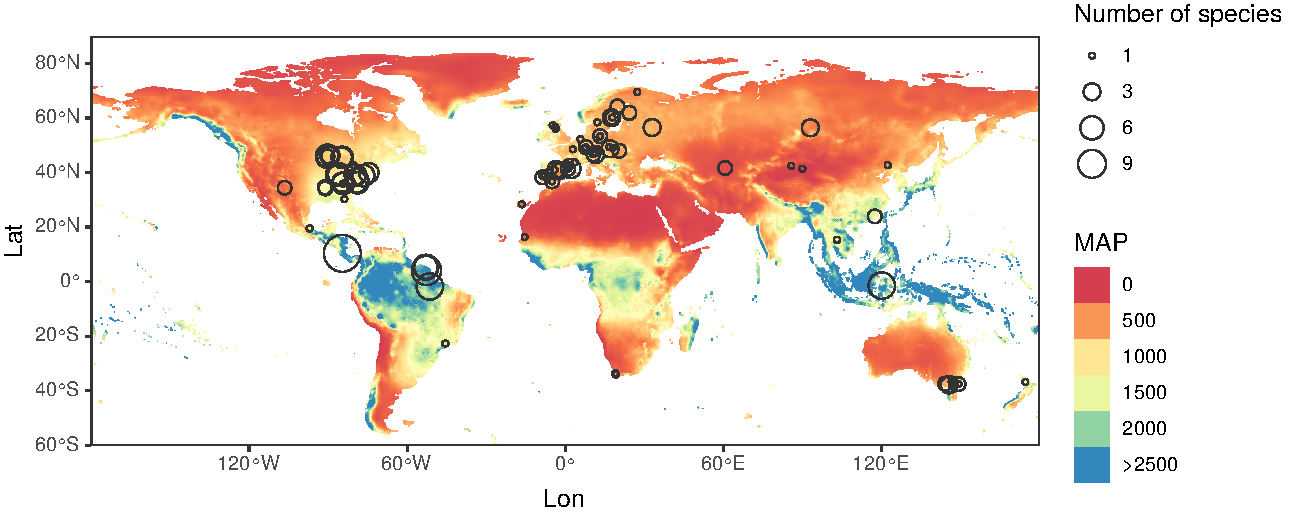
\includegraphics[width=1\linewidth]{figure/CH5/Figure_1} 

}

\caption[Distribution of the plots from the SAPFLUXNET database included in this study.]{Distribution of the plots from the SAPFLUXNET database included in this study. Size of the dots represent the number of different species in the plot. Color gradient show mean annual precipitation (MAP).}\label{fig:ch5fig1}
\end{figure}
\subsection{Evaporative demand and soil water availability
data}\label{evaporative-demand-and-soil-water-availability-data}

We used vapour pressure deficit (VPD) and soil water content (SWC) as
proxies of evaporative demand and soil water availability, respectively.
Similar to SFD, VPD was obtained from on-site sub-daily measurements
from SAPFLUXNET averaged to daytime values. Soil water content (SWC;
v/v) was obtained from the 15-30 cm depth layer at 12 am from the
ERA5-land re-analysis product (Copernicus Climate Change Service (C3S),
2019) at 9x9 km resolution. We used ERA5-land re-analyses instead of
on-site SWC measures in order to maximize the number of plots and
species included in the study, since SWC data were missing in 44\% of
the SAPFLUXNET data-sets included in this study. In addition, ERA5-land
had longer time series (1980 to 2019). We validated the use of ERA5-land
data using a linear mixed-model (LMM) regression between ERA5-land and
on-site shallow SWC measurements by letting random intercepts and slopes
of the response vary by site (n observations = 32815; n plots = 71;
\(R^2\)conditional = 0.97, \(R^2\)marginal = 0.26).\par

To complement SWC, we also calculated relative extractable water (REW),
as a normalized measure of soil water availability, as follows:
\begin{equation}
REW_{j,i} = \frac{SWC_{j,i} - SWC_{min}}{SWC_{max} - SWC_{min}}
\end{equation}
where \(REW_{j,i}\) and \(SWC_{j,i}\) are plot (\(j\)) daily (\(i\))
values, and SWCmax and SWCmin, the overall maximum and minimum SWC
measured at a plot, respectively. REW takes values between 0 and 1,
being 0 the absolute plot lowest SWC and 1 being the highest.\par

\subsection{Data filtering}\label{data-filtering}

We restricted the analysis to periods without potential phenological
changes in leaf area to minimize variations in conductance unrelated to
VPD and SWC changes. In the absence of detailed plot-specific
observations, we excluded all data for periods comprised between 15 days
prior to the first day with temperatures below 0ºC and 30 days following
the last day under 0ºC, respectively, during the cold seasons of each
plot site (similarly to Novick et al., 2016). To prevent potential
artefacts due to unstable weather conditions in the calculation of
whole-tree canopy conductance (Ewers \& Oren, 2000) or in the estimation
of model parameters, we filtered out days when SWC increased (rainy
days), as well as days when daytime-averaged VPD was below 0.3 kPa
(Anderegg et al., 2018). To ensure sufficiently contrasting conditions
of evaporative demand and soil water availability, we also discarded
species with both VPD ranges below 0.5 kPa and SWC ranges below 0.05 (n
= 8 species).\par

After data filtering, the study covers a large geographic area
\textbackslash{}fdash being Europe and the east of North America
especially well represented (Fig 1)\textbackslash{}fdash and a wide
range of climate conditions, with MAP values ranging from 14 mm to 3626
mm (mean \textbackslash{}pm SD = 953 mm \textbackslash{}pm 545 mm). Out
of the 142 species used in the analyses, 116 were angiosperms and 26
gymnosperms. The number of trees per species ranges from 215 trees
(Pinus sylvestris) to 1 (this being the case for 23 species) (Table S2).
Tree species-level heights (H) range from 2 m (Coprosma quadrifida) to
40 m (Carya glabra) (mean \textbackslash{}pm SD = 21 m
\textbackslash{}pm 9.75 m).\par

\subsection{Whole-tree canopy conductance
calculation}\label{whole-tree-canopy-conductance-calculation}

Daytime SFD was transformed from
{[}\(cm^3 \: cm_{Asw}^{-2} \: h^{-1}\){]} to
{[}\(kg \: m_{Asw}^{-2} \: s^{-1}\){]} and converted to daily whole-tree
canopy conductance normalized per unit of sapwood area
\(G_{\text{Asw}}\)\$ using Phillips and Oren (1998) and unit
transformations (eq.2).
\begin{equation}
G_{Asw,j,i,k} = \frac{115.8 + 0.4236 \: T_{j , i} \cdot SFD_{j , i , k}}{VPD_{j,i}}\cdot 44.6 \cdot \frac{273}{(273 + T_{j,i})} \cdot \frac{101.325 \: e^{0.00012 \cdot h_i}}{101.325}
\end{equation}
Where \(SFD_{j,i,k}\) is sap flux density value of each plot (\(j\)),
day (\(i\)), and tree (\(k\)); \(T_{j,i}\) is the temperature,
\(VPD_{j,i}\) is the daytime vapor pressure deficit and \(h\) is the
altitude of each plot site. When \(h\) was not available it was obtained
from The Shuttle Radar Topography Mission (SRTM) (Earth Resources
Observation And Science (EROS) Center, 2017) (n = 2 plots).\par

The conductance obtained using eq. 2 is considered a good proxy of the
tree-level stomatal conductance under the assumption that the canopy and
the atmosphere are well-coupled, i.e., when the aerodynamic conductance
is much larger than the stomatal conductance. Although this is generally
assumed in sap flow studies for both needleleaf and even broadleaf
species, there is evidence that coupling may only be partial in some
cases (Magnani et al., 1998; De Kauwe et al., 2017). Therefore, we also
calculated whole-tree stomatal conductance (\(G_{\text{Asw}}^{'}\)) by
removing the contribution of aerodynamic conductance in a subset of
plots-species (n plots = 64; n species = 47) where wind speed data were
available in SAPFLUXNET (see supplementary material for details, Chu et
al., 2018; Tan et al., 2019). We also related the environmental
sensitivity of \(G_{\text{Asw}}^{'}\) to the hydraulic and allocation
traits (see Statistical analyses section below) to assess the potential
impact of partial canopy-atmosphere coupling on our results.\par

\subsection{Traits and climatic data}\label{traits-and-climatic-data}

Species-level traits (\textbar{}\(\Psi_{P50}\)\textbar{}, \(Hv\),
\(K_s\), \textbar{}\(\Psi_{TLP}\)\textbar{}, \(R_{depth}\) and \(L_s\))
were taken from HydraTry (Mencuccini et al., 2019b; Sanchez‐Martinez et
al., 2020) and the Global Leaf Size Dataset (Wright et al., 2017) (Table
S2). \textbar{}\(\Psi_{P50}\)\textbar{}, \(Hv\), \(K_s\) and \(L_s\)
were log-transformed to achieve normality. In addition, we obtained tree
species-level height (H) as the average of SAPFLUXNET actual tree
heights, with the number of tree-days with available sap flow values as
weighting factor. The height of the stand was used when the actual
height of a tree was not available (792 out of 1929 trees).\par

To account for climatic effects on the species' water use parameters and
on water relation traits, we used mean annual precipitation (MAP), mean
annual temperature (MAT) and an aridity index defined as precipitation
over potential evapotranspiration (PPET) (Fig. 1, Fig. S6, Fig. S7).
However, for simplicity, we only included MAP in the analyses since for
the species in the study MAP was strongly correlated with PPET (\(r\) =
0.94) and MAT (\(r\) = 0.76), whereas PPET and MAT correlation was lower
(\(r\) = 0.56). MAP and MAT were obtained for all study plots from the
CHELSA data set (1x1 km resolution) (Karger et al., 2017) and averaged
at the species level weighting by the number of tree-days. PPET were
obtained from CGIAR-CSI Global Aridity index (Trabucco \& Zomer,
2019).\par

\subsection{\texorpdfstring{\(\textbf{G}_{\textbf{Asw}}\) sensitivity to
soil water availability and water
demand}{\textbackslash{}textbf\{G\}\_\{\textbackslash{}textbf\{Asw\}\} sensitivity to soil water availability and water demand}}\label{textbfg_textbfasw-sensitivity-to-soil-water-availability-and-water-demand}

In some species, \(G_{\text{Asw}}\) measurements were distributed very
heterogeneously throughout the range of VPD or SWC. To avoid the issues
associated with such unbalanced distributions we used binned data.
Specifically, we calculated the average of \(G_{\text{Asw}}\)
measurements comprised into 0.2 kPa VPD intervals and five bins spanning
the plot-species specific SWC range. For each summarized
\(G_{\text{Asw}}\) we defined a characteristic VPD and SWC as the
average values of VPD and SWC of the data in the bin. The summarized
values of \(G_{\text{Asw}}\) were fitted using LMM as a function of the
logarithm of VPD (ln(VPD)) and the logarithm of SWC (ln(SWC)) as
additive explanatory variables using uncorrelated random slopes for each
species and a random intercept for each tree nested in each species. We
log-transformed the independent variables to linearise the relationships
and ensure normal residuals. LMMs were fitted using the lmer function
from the lme4 R package (Bates et al., 2015). Using the coef function
from lme4 we obtained species parameters \(\beta_{\text{VPD}}\) and
\(\beta_{\text{SWC}}\) (i.e.~species \(G_{\text{Asw}}\) sensitivity to
VPD and to SWC, respectively), with higher values of
\(\beta_{\text{VPD}}\) or \(\beta_{\text{SWC}}\) meaning stronger G
reductions with increasing VPD or decreasing SWC, respectively. In
addition, a reference \(G_{\text{Asw}}\) (\(G_{\text{REF}}\))
characterizing water use under standard conditions for each species, was
predicted setting VPD = 1 kPa and SWC = 0.5 m3 m-3 (which is close to
the average maximum of all sites). Complementary models were also fitted
following the same procedure but with REW instead of SWC, so that soil
water content variability was normalized across sites. Additional models
were also fitted using canopy stomatal conductance
(\(G_{\text{Asw}}^{'}\)) as response variable. Finally, to remove
parameter outliers, species with \(G_{\text{REF}}\) ,
\(\beta_{\text{VPD}}\) or \(\beta_{\text{SWC}}\) outside the 99.9
percentile of their normal distribution were excluded from subsequent
analyses (2 out of 142 species excluded).\par

\subsection{Statistical analyses}\label{statistical-analyses}

We tested whether water use regulation traits (\(G_{\text{REF}}\),
\(\beta_{\text{VPD}}\) and \(\beta_{\text{SWC}}\)) differ between
angiosperms and gymnosperms using a simple linear model. Next, we
constructed bi-variate linear relationships between species' fitted
parameters and species' water relations traits. Furthermore, we repeated
these linear relationships by adding MAP and H as predictors and
applying a stepwise model selection, to discern whether the effect of
the traits remained significant once these new variables were added to
the model. In all the analyses we used the number of species' tree-days
as a weighting factor.\par

Finally, we performed a path analysis using the SEM function of the
lavaan R package (Rosseel, 2012). Path analysis accounts for direct and
indirect dependencies among variables. To account for the coordinated
effect of the species' relations traits and to maximize the number of
species (106 species), we imputed species' trait missing values (Table
S2) using the imputePCA function of the package missMDA (Josse \&
Husson, 2016) and then performed a Principal Component Analysis (PCA) to
extract the two main principal components (Fig. S1). A single path model
was built including the three parameters describing \(G_{\text{Asw}}\)
behaviour (\(G_{\text{REF}}\), \(\beta_{\text{VPD}}\) and
\(\beta_{\text{SWC}}\)) as response variables and using MAP, \(H\) and
the two dimensions of the traits' PCA as explanatory variables. In
addition to direct relationships, indirect effects of MAP and \(H\) on
the fitted parameters were also included through their effect on the PCA
dimensions (Liu et al., 2019). We also accounted for the effect of MAP
on \(H\). We included the number of tree-days per species as a weighting
factor in the model. We performed a model selection procedure to include
only paths with at least moderately strong support (P \textless{} 0.1).
Finally, we also checked that the fit of the final model was not
significantly different from the saturated model using the lavTestLRT
function of the lavaan R package (Rosseel, 2012) with Satorra and
Bentler (2001) approximation. All variables were standardized before
fitting the path models. All the analyses of the study were performed in
R3.6.1 (R Core Team, 2018).\par
\begin{figure}[H]

{\centering 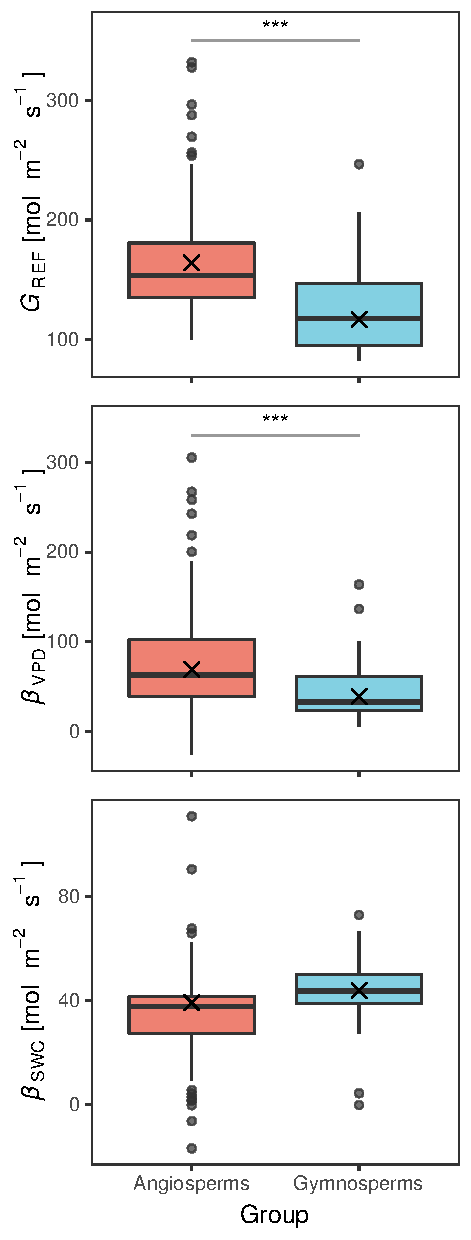
\includegraphics[width=0.5\linewidth]{figure/CH5/Figure_2} 

}

\caption[Boxplots of water use parameters for both Angiosperms and Gymnosperms.]{Boxplots of water use parameters for both Angiosperms and Gymnosperms. Crosses are weighted means of the parameters.}\label{fig:ch5fig2}
\end{figure}
\section{Results}\label{results}

\subsection{Water use parameters and differences between angiosperms and
gymnosperms}\label{water-use-parameters-and-differences-between-angiosperms-and-gymnosperms}

The model used to obtain water use parameters explained a 59.8\% of the
total conditional variance in the original data. Reference conductance
(\(G_{\text{REF}}\)) across species ranged between 82.4
\(mol\: m_{Asw}^{-2}\: s^{-1}\) (Juniperus monosperma) and 333
\(mol\: m_{Asw}^{-2}\: s^{-1}\) (Acacia longifolia),
\(\beta_{\text{VPD}}\) between -26 \(mol\: m_{Asw}^{-2}\: s^{-1}\)
(Avicennia marina) and 306 \(mol\: m_{Asw}^{-2}\: s^{-1}\) (Ulmus
americana) and \(\beta_{\text{SWC}}\) between -17.3
\(mol\: m_{Asw}^{-2}\: s^{-1}\) (Acer saccharum) and 112
\(mol \: m_{Asw}^{-2}\: s^{-1}\) (Acacia longifolia) (Fig. S2 -- S3 --
S4). Most species showed declining G with increasing VPD (positive
\(\beta_{\text{VPD}}\)) and increasing G with increasing SWC (positive
\(\beta_{\text{SWC}}\)).\par

Species showing opposite responses were two temperate (Acer saccharum,
Quercus petraea), one tropical (Ampelocera macrocarpa) and a mangrove
(Avicennia marina) species that showed negative sensitivities to one of
the variables (Fig. S2). Mean \(G_{\text{REF}}\) and
\(\beta_{\text{VPD}}\) were significantly higher for angiosperms than
for gymnosperms (Fig. 2). However, there were no differences in
\(\beta_{\text{SWC}}\) between angiosperms and gymnosperms. Across all
species (including angiosperms and gymnosperms), \(G_{\text{REF}}\) and
\(\beta_{\text{VPD}}\) were strongly and positively correlated (\(r\) =
0.75; with a weighted slope of 0.67; Fig. S5), being the species with
high \(G_{\text{REF}}\) more sensitive to VPD, but strong correlations
were not found between \(G_{\text{REF}}\) and \(\beta_{\text{SWC}}\) or
between \(\beta_{\text{VPD}}\) and \(\beta_{\text{SWC}}\)
(\textbar{}\(r\)\textbar{} \textless{} 0.34 in both cases). When
comparing water use parameters calculated considering and not
considering aerodynamic conductance, we found that \(G_{\text{REF}}\)
was strongly correlated to \(G_{\text{REF}}^{'}\) (\(r\) = 0.8);
however, \(\beta_{\text{VPD}}\) and \(\beta_{\text{VPD}}^{'}\) were
poorly correlated (\(r\) = 0.26) while \(\beta_{\text{SWC}}\) and
\(\beta_{\text{SWC}}^{'}\) showed no significant correlation.\par
\begin{figure}[H]

{\centering 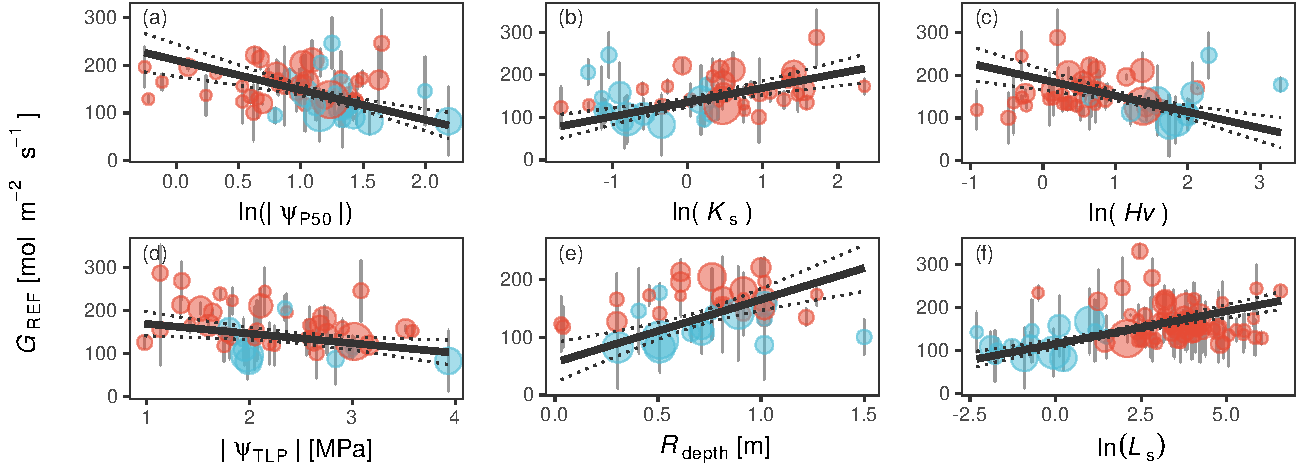
\includegraphics[width=1\linewidth]{figure/CH5/Figure_3} 

}

\caption[Bi-variate relationships between $G_{\text{REF}}$ water relations traits.]{Bi-variate relationships between $G_{\text{REF}}$ water relations traits. Individual water relation traits are shown in different panels: (a) logarithm of absolute water potential at 50\% water conductivity loss, (b) logarithm of maximum sapwood water conductivity, (c) logarithm of Huber value, (d) absolute water potential at turgor-loss point, (e) rooting depth and (f) logarithm of individual leaf area. Black continuous lines depict significant linear relationships (Table 2) and the dashed lines represent the 95\% confidence intervals of the models. Red dots are angiosperms and blue dots are gymnosperms. Size of the points is equivalent to the number of tree-days of the species. Vertical lines are the posterior standard deviation of the parameters calculated using REsim function of merTools package (Knowles \& Frederick, 2016).}\label{fig:ch5fig3}
\end{figure}
\subsection{Coordination with hydraulic and allocation
traits}\label{coordination-with-hydraulic-and-allocation-traits}

In the bi-variate models relating \(G_{\text{REF}}\) with hydraulic and
morphological traits, we found that \(G_{\text{REF}}\) showed a negative
relationship with \textbar{}\(\Psi_{P50}\)\textbar{}, \(Hv\) and
\textbar{}\(\Psi_{TLP}\)\textbar{} (Table 2 and Fig. 3a,c,d), whereby
species more resistant to embolism, with higher allocation to the
sapwood relative to leaves and with more negative turgor-loss pressures
showed lower \(G_{\text{REF}}\). Furthermore, \(G_{\text{REF}}\) was
positively related to \(K_s\), \(R_{depth}\) and \(L_s\) (Table 2 and
Fig. 3b,e,f), with species with efficient xylem, deeper roots and bigger
leaves showing higher \(G_{\text{REF}}\). For these traits, \(L_s\) was
the one explaining the largest fraction of \(G_{\text{REF}}\)
variability (\(R^2\) = 0.39). With the exception of \(\Psi_{TLP}\),
these relationships remained significant also for \(G_{\text{Asw}}^{'}\)
(Table S3).\par
\begin{table}

\caption[Results of the bi-variate linear models relating water use parameters and water relations traits]{\label{tab:Ch5T2}Results of the bi-variate linear models relating water use parameters ($G_{\text{REF}}$, $\beta_{\text{VPD}}$, $\beta_{\text{SWC}}$) and water relations traits. Parameters are explained by individual traits using simple linear models using number of species-days as weighting factor.}
\centering
\resizebox{\linewidth}{!}{
\fontsize{10}{12}\selectfont
\begin{tabular}[t]{>{\raggedright\arraybackslash}p{2cm}>{\raggedright\arraybackslash}p{3cm}rllr}
\toprule
Water use parameter & Water relations Traits & N species & Intercept & Slope & $R^{2}$\\
\midrule
 & $ln(\rvert\Psi_{\text{P50}}\rvert)$ & 55 & 210.701*** & -62.724 *** & 0.282\\
\cmidrule{2-6}
 & $ln(K_\text{s})$ & 43 & 135.527*** & 33.614 *** & 0.338\\
\cmidrule{2-6}
 & $ln(Hv)$ & 49 & 189.439*** & -37.602 *** & 0.285\\
\cmidrule{2-6}
 & $\rvert\Psi_{\text{TLP}}\rvert$ & 48 & 191.764*** & -22.702 * & 0.112\\
\cmidrule{2-6}
 & $R_{\text{depth}}$ & 37 & 56.204** & 109.296 *** & 0.366\\
\cmidrule{2-6}
\multirow{-6}{*}{\raggedright\arraybackslash $G_{\text{REF}}$} & $ln(L_\text{s})$ & 86 & 115.537*** & 15.28 *** & 0.391\\
\cmidrule{1-6}
 & $ln(\rvert\Psi_{\text{P50}}\rvert)$ & 55 & 109.201*** & -47.716 *** & 0.240\\
\cmidrule{2-6}
 & $ln(K_\text{s})$ & 43 & 50.199*** & 20.427 ** & 0.180\\
\cmidrule{2-6}
 & $ln(Hv)$ & 49 & 96.503*** & -33.817 *** & 0.363\\
\cmidrule{2-6}
 & $\rvert\Psi_{\text{TLP}}\rvert$ & 48 & 80.321*** & -12.209 . & 0.040\\
\cmidrule{2-6}
 & $R_{\text{depth}}$ & 37 & -2.190 ns & 80.383 *** & 0.260\\
\cmidrule{2-6}
\multirow{-6}{*}{\raggedright\arraybackslash $\beta_{\text{VPD}}$} & $ln(L_\text{s})$ & 86 & 34.577*** & 11.219 *** & 0.327\\
\cmidrule{1-6}
 & $ln(\rvert\Psi_{\text{P50}}\rvert)$ & 55 & 16.103 ns & 19.327 * & 0.059\\
\cmidrule{2-6}
 & $ln(K_\text{s})$ & 43 & 42.113*** & -5.021 ns & 0.000\\
\cmidrule{2-6}
 & $ln(Hv)$ & 49 & 23.952** & 13.586 * & 0.088\\
\cmidrule{2-6}
 & $\rvert\Psi_{\text{TLP}}\rvert$ & 48 & 40.468** & 1.052 ns & 0.000\\
\cmidrule{2-6}
 & $R_{\text{depth}}$ & 37 & 53.851*** & -28.471 . & 0.051\\
\cmidrule{2-6}
\multirow{-6}{*}{\raggedright\arraybackslash $\beta_{\text{SWC}}$} & $ln(L_\text{s})$ & 86 & 51.112*** & -4.095 ** & 0.087\\
\bottomrule
\multicolumn{6}{l}{\textsuperscript{} Statistical significant levels: "." p<0.1 ; "*" p<0.05; "**" p<0.01; "***" p<0.001; ns not significant.}\\
\end{tabular}}
\end{table}
\(\beta_{\text{VPD}}\) was negatively related with
\textbar{}\(\Psi_{P50}\)\textbar{} and \(Hv\) and positively with
\(K_s\) (Table 2 and Fig. 4a,b,c), i.e., species with less safe and more
efficient xylem present higher sensitivity to VPD, and hence more strict
stomatal control as atmospheric water demand increases.
\(\beta_{\text{VPD}}\) was also positively related to \(R_{depth}\) and
\(L_s\) (Table 2 and Fig. 4e,f), indicating that deeper roots and larger
leaves were associated to higher stomatal sensitivity to VPD. Absolute
turgor-loss point (\textbar{}\(\Psi_{TLP}\)\textbar{}) was weakly
negatively related with \(\beta_{\text{VPD}}\) (p value = 0.093; Table
2). \(Hv\) and \(L_s\) were the traits explaining most of
\(\beta_{\text{VPD}}\) variability (\(R^2\) = 0.36 and \(R^2\) = 0.33,
respectively). With the exception of \(\Psi_{TLP}\), these relationships
remained significant also for \(G_{\text{Asw}}^{'}\) (Table S3).\par
\begin{figure}[hbt!]

{\centering 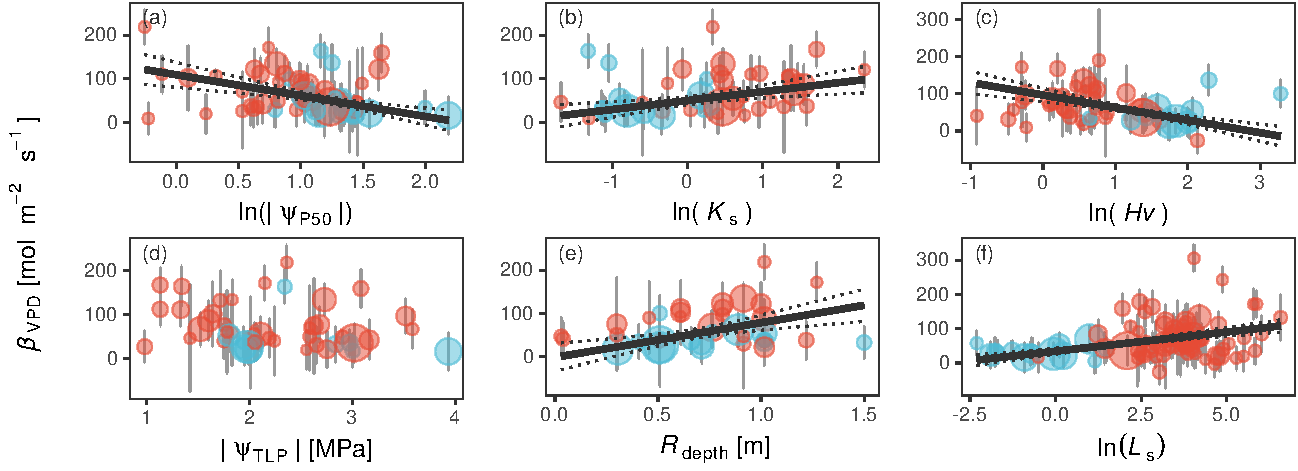
\includegraphics[width=1\linewidth]{figure/CH5/Figure_4} 

}

\caption[Bi-variate relationships between $\beta_{\text{VPD}}$ water relations traits.]{Bi-variate relationships between $\beta_{\text{VPD}}$ water relations traits. Individual water relation traits are shown in different panels: (a) logarithm of absolute water potential at 50\% water conductivity loss, (b) logarithm of maximum sapwood water conductivity, (c) logarithm of Huber value, (d) absolute water potential at turgor-loss point, (e) rooting depth and (f) logarithm of individual leaf area. Black continuous lines depict significant linear relationships (Table 2) and the dashed lines represent the 95\% confidence intervals of the models. Red dots are angiosperms and blue dots are gymnosperms. Size of the points is equivalent to the number of tree-days of the species. Vertical lines are the posterior standard deviation of the parameters calculated using REsim function of merTools package (Knowles \& Frederick, 2016).}\label{fig:ch5fig4}
\end{figure}
\(\beta_{\text{SWC}}\) was positively related to
\textbar{}\(\Psi_{P50}\)\textbar{} and \(Hv\) (Table 2 and Fig. 5a,c),
i.e., species with higher resistance to embolism and larger ratios of
sapwood to leaf area were more sensitive to soil water depletion. In
addition, species with larger leaves (\(L_s\)) and, marginally (p value
= 0.095), with deeper roots (\(R_{depth}\)) were less sensitive to soil
water stress (Table 2 and Fig. 5e,f). In general, water relations traits
explained a lower proportion (at most 9\%) of the variability in
\(\beta_{\text{SWC}}\) than of \(G_{\text{REF}}\) or
\(\beta_{\text{VPD}}\). However, we should treat relationships between
\(\beta_{\text{SWC}}\) and \textbar{}\(\Psi_{P50}\)\textbar{}, \(Hv\)
and \(R_{depth}\) with caution, since they all become non-significant
when aerodynamic conductance was taken into account (Table S3) or when
REW was used instead of SWC (Table S3). Furthermore, when REW was used
instead of SWC, all soil moisture sensitivity-trait relationships became
non-significant (Table S4).\par
\begin{figure}[hbt!]

{\centering 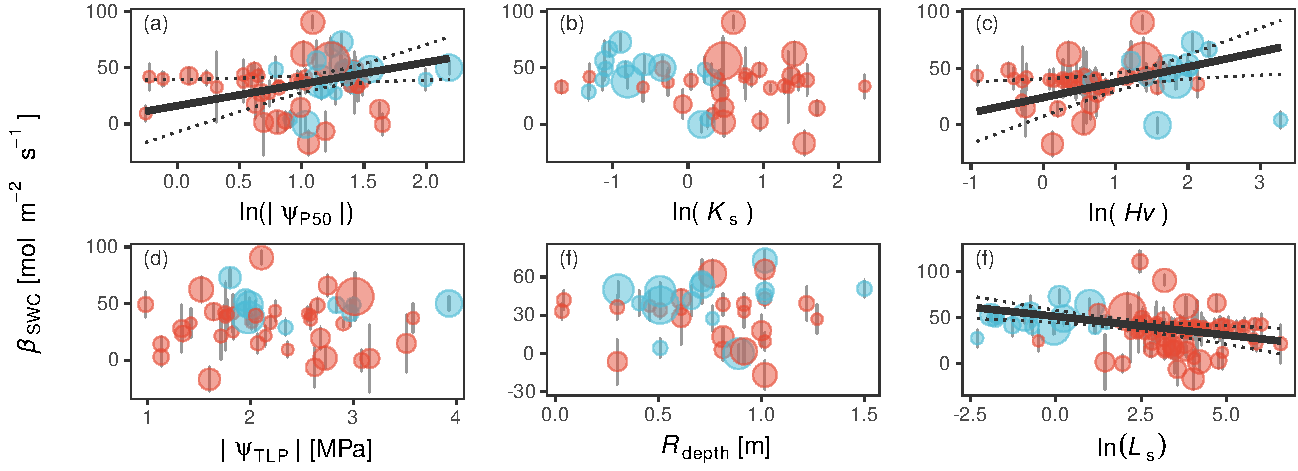
\includegraphics[width=1\linewidth]{figure/CH5/Figure_5} 

}

\caption[Bi-variate relationships between $\beta_{\text{SWC}}$ water relations traits.]{Bi-variate relationships between $\beta_{\text{SWC}}$ water relations traits. Individual water relation traits are shown in different panels: (a) logarithm of absolute water potential at 50\% water conductivity loss, (b) logarithm of maximum sapwood water conductivity, (c) logarithm of Huber value, (d) absolute water potential at turgor-loss point, (e) rooting depth and (f) logarithm of individual leaf area. Black continuous lines depict significant linear relationships (Table 2) and the dashed lines represent the 95\% confidence intervals of the models. Red dots are angiosperms and blue dots are gymnosperms. Size of the points is equivalent to the number of tree-days of the species. Vertical lines are the posterior standard deviation of the parameters calculated using REsim function of merTools package (Knowles \& Frederick, 2016).}\label{fig:ch5fig5}
\end{figure}
\begin{table}

\caption[Results of the bi-variate linear models relating water use parameters, water relations traits, climate and tree height.]{\label{tab:Ch5T3}Results of the bi-variate linear models relating water use parameters ($G_{\text{REF}}$, $\beta_{\text{VPD}}$, $\beta_{\text{SWC}}$), water relations traits, climate and tree height. Water use parameters are explained using simple linear models with number of species-days as weighting factor. $\beta$ column values are the slopes for each explanatory variable. N species = number of species included. NI = not included variable after model selection.}
\centering
\resizebox{\linewidth}{!}{
\fontsize{10}{12}\selectfont
\begin{tabular}[t]{>{\raggedright\arraybackslash}p{2cm}>{\raggedright\arraybackslash}p{2.5cm}rllllr}
\toprule
Water use parameter & Water relations Traits & N species & Intercept & $\beta_{\text{trait}}$ & $\beta_{\text{MAP}}$ & $\beta_{\text{H}}$ & $R^{2}$\\
\midrule
 & $ln(\rvert\Psi_{\text{P50}}\rvert)$ & 54 & 173.6 *** & -48.549 ** & NI & 1.418 * & 0.325\\
\cmidrule{2-8}
 & $ln(K_\text{s})$ & 42 & 109.773 *** & 30.731 *** & NI & 1.822 * & 0.423\\
\cmidrule{2-8}
 & $ln(Hv)$ & 43 & 162.178 *** & -32.21 ** & NI & 1.448 . & 0.332\\
\cmidrule{2-8}
 & $\rvert\Psi_{\text{TLP}}\rvert$ & 47 & 66.861 *** & NI & 0.057 * & 1.962 * & 0.346\\
\cmidrule{2-8}
 & $R_{\text{depth}}$ & 36 & 41.932 * & 88.301 *** & NI & 1.802 * & 0.448\\
\cmidrule{2-8}
\multirow{-6}{*}{\raggedright\arraybackslash $G_{\text{REF}}$} & $ln(L_\text{s})$ & 80 & 98.531 *** & 13.389 *** & NI & 1.384 ** & 0.450\\
\cmidrule{1-8}
 & $ln(\rvert\Psi_{\text{P50}}\rvert)$ & 54 & 70.665 *** & -32.97 ** & NI & 1.468 * & 0.317\\
\cmidrule{2-8}
 & $ln(K_\text{s})$ & 42 & 25.16 * & 17.444 ** & NI & 1.768 ** & 0.303\\
\cmidrule{2-8}
 & $ln(Hv)$ & 43 & 73.255 *** & -28.931 *** & NI & 1.197 * & 0.408\\
\cmidrule{2-8}
 & $\rvert\Psi_{\text{TLP}}\rvert$ & 47 & 16.363 . & NI & NI & 2.502 *** & 0.291\\
\cmidrule{2-8}
 & $R_{\text{depth}}$ & 36 & -18.282 ns & 56.571 * & NI & 2.034 ** & 0.412\\
\cmidrule{2-8}
\multirow{-6}{*}{\raggedright\arraybackslash $\beta_{\text{VPD}}$} & $ln(L_\text{s})$ & 80 & 16.099 * & 8.955 *** & NI & 1.512 *** & 0.429\\
\cmidrule{1-8}
 & $ln(\rvert\Psi_{\text{P50}}\rvert)$ & 54 & 62.606 *** & NI & -0.029 * & NI & 0.088\\
\cmidrule{2-8}
 & $ln(K_\text{s})$ & 42 & 73.319 *** & NI & -0.038 ** & NI & 0.142\\
\cmidrule{2-8}
 & $ln(Hv)$ & 43 & 50.25 ** & 10.221 ns & -0.026 . & NI & 0.149\\
\cmidrule{2-8}
 & $\rvert\Psi_{\text{TLP}}\rvert$ & 47 & 55.33 *** & NI & NI & -0.903 * & 0.067\\
\cmidrule{2-8}
 & $R_{\text{depth}}$ & 36 & 62.889 *** & NI & -0.037 ** & NI & 0.213\\
\cmidrule{2-8}
\multirow{-6}{*}{\raggedright\arraybackslash $\beta_{\text{SWC}}$} & $ln(L_\text{s})$ & 80 & 44.671 *** & -5.002 ** & 0.025 * & -0.749 * & 0.142\\
\bottomrule
\multicolumn{8}{l}{\textsuperscript{} Statistical significant levels: "." p<0.1 ; "*" p<0.05; "**" p<0.01; "***" p<0.001; ns not significant.}\\
\end{tabular}}
\end{table}
Ecological factors associated with water use parameters and coordination
When the coordination between water use parameters and water relations
traits was assessed while also accounting for the effects of MAP (mean
annual precipitation) and \(H\) (tree species-level mean height), most
of the relationships described in the previous section remained
significant, with only three exceptions. The relationships that were no
longer observed corresponded to the effect of \(\Psi_{TLP}\) on
\(G_{\text{REF}}\) and the effects of \textbar{}\(\Psi_{P50}\)\textbar{}
and \(Hv\) on \(\beta_{\text{SWC}}\) (Table 3). In these models, MAP was
the variable that explained most of the variability in stomatal
responses to soil water (\(\beta_{\text{SWC}}\)), with generally lower
sensitivity to SWC in locations with high MAP (Table 3), although this
effect reversed in the \(L_s\) model. However, when models were
calculated using \(\beta_{\text{SWC}}^{'}\), MAP effects were all
negative (Table S5). On the other hand, MAP was largely unrelated to
\(G_{\text{REF}}\) and \(\beta_{\text{VPD}}\) in most of the
\(G_{\text{REF}}\) and \(\beta_{\text{VPD}}\) models (Table 3). Finally,
our results show that taller trees tend to have higher
\(G_{\text{REF}}\) and higher sensitivity to VPD
(\(\beta_{\text{VPD}}\)), however, when \(G_{\text{REF}}\) was obtained
from \(G_{\text{Asw}}^{'}\) (i.e. \(G_{REF}^{'}\)), \(H\) was not
selected in the final models (Table S5). The relationship between \(H\)
and soil drought sensitivity (\(\beta_{\text{SWC}}\)) was less clear,
since it was significantly negative in only two of the models (Table 3),
suggesting higher sensitivity to soil drought in shorter trees. However
when aerodynamic coupling was taken into account, the relationship was
inverted and taller trees had higher sensitivity to SWC (Table S5).\par

The two main dimensions of the PCA analyses describing water relations
trait coordination explained a 69.8\% of the total variance (Fig. S1).
The primary PCA dimension (Dim1; 56.8\% of variance) could be
interpreted as a safety-efficiency trade-off axis, whereby positive
values are related to elevated \(K_s\), large \(L_s\), deep roots, low
\(Hv\) and low \textbar{}\(\Psi_{P50}\)\textbar{}. The second PCA
dimension (Dim2; 13\% of variance) was associated to leaf turgor-loss
pressure (\(\Psi_{TLP}\)), with positive values related to high
\textbar{}\(\Psi_{TLP}\)\textbar{} levels and, to a lower extent, deeper
roots.\par
\begin{figure}[hbt!]

{\centering 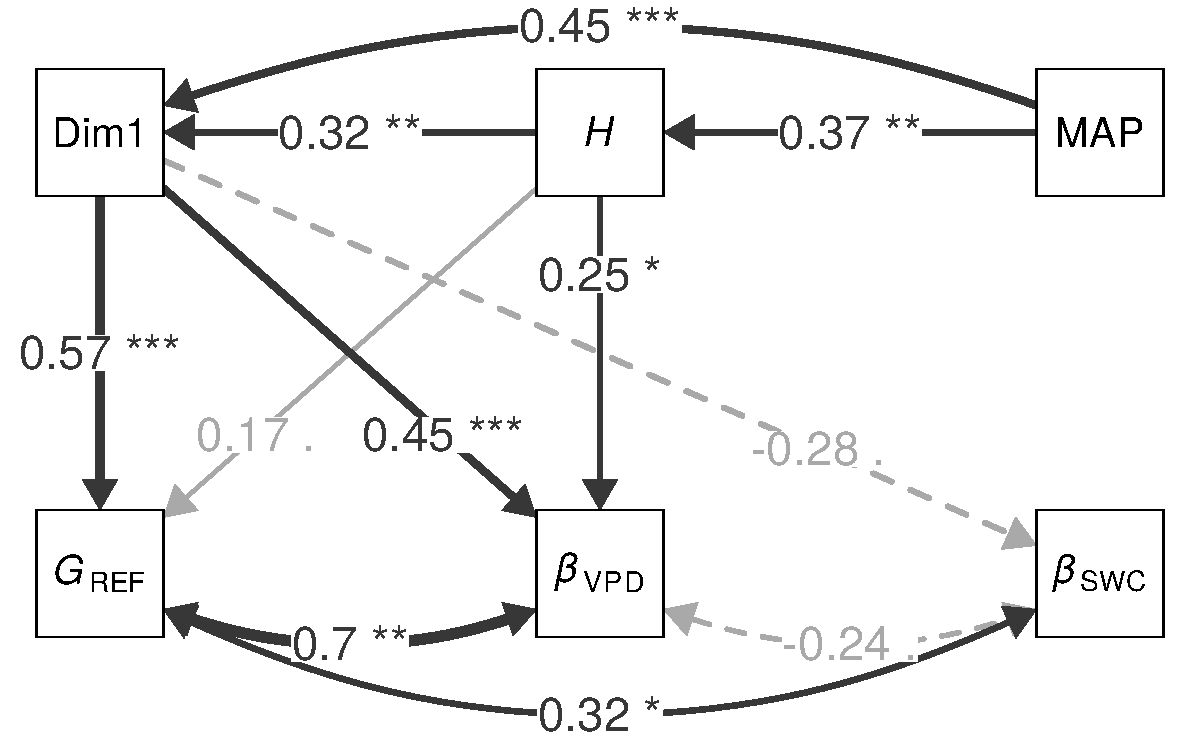
\includegraphics[width=0.8\linewidth]{figure/CH5/Figure_6} 

}

\caption[Path analyses of species-specific water use parameters.]{Path analyses of species-specific water use parameters explained by mean annual precipitation (MAP), tree height ($H$) and coordinated hydraulic traits Dim1. Dim1 is the hydraulic traits’ PCA dimension 1 (Fig. S1). Positive Dim1 values are mainly related to efficient water use strategies, while negative to safety strategies. Dim2 was not selected in the final model. Arrow labels are standardized parameters. Continuous lines are positive relationships while dashed lines are negative relationships. Black and grey lines are significant and marginally significant relationships, respectively. Statistical significant levels: ., P < 0.1 ; *, P < 0.05; **, P < 0.01; ***, P < 0.001}\label{fig:ch5fig6}
\end{figure}
In the path analyses, efficiency traits (positive PCA Dim1 values) were
significantly related to high annual precipitation (high MAP) and to
taller trees (large \(H\)) (Fig. 6). Also, \(H\) increased with MAP.
\(G_{\text{REF}}\) was positively associated with Dim1 (Fig. 6) and
taller trees also had marginally higher \(G_{\text{REF}}\) (Fig. 6).
Similarly, higher \(\beta_{\text{VPD}}\) (i.e., higher VPD sensitivity)
was positively related to efficient water transport (Dim1) and to \(H\)
(Fig. 6). Sensitivity to SWC (\(\beta_{\text{SWC}}\)) showed a marginal,
negative relationship with Dim1, so that sensitivity increased with
xylem resistance to embolism (Fig. 6). Finally, \(G_{\text{REF}}\)
co-varied positively with \(\beta_{\text{VPD}}\) and
\(\beta_{\text{SWC}}\), implying that as \(G_{\text{REF}}\) increases so
do \(\beta_{\text{VPD}}\) and \(\beta_{\text{SWC}}\) (Fig. 6, Fig. S5).
The second dimension of the PCA was not included in the final path
model, suggesting a lack of coordination between \(\Psi_{TLP}\) and
water use parameters.\par

\section{Discussion}\label{discussion}

In this study, we present a novel analysis linking organ-level traits
with whole-plant water use strategies at the global scale, made possible
by the compilation of the first global sap flow database. We provide
evidence of a coordination between water relations traits and water use
parameters (\(G_{\text{REF}}\), \(\beta_{\text{VPD}}\) and
\(\beta_{\text{SWC}}\)), while accounting for the effects of climate and
tree size. Some water use and trait associations were explained by
climate affiliations of species, but most relationships between water
use and water relations traits remained after accounting for climate and
tree size effects. As any synthesis effort of this magnitude based on
diverse data sources, our study presents several limitations. First, sap
flow data used to estimate G carry some uncertainty issues, although
these may be less relevant for assessing environmental responses as we
do here than for characterizing absolute values (Flo et al., 2019).
Second, SAPFLUXNET may have an incomplete coverage of global forest
ecosystems (Fig. 1, Poyatos et al., 2020). Third, highly non-linear or
threshold-based SWC responses may be difficult to capture, especially
when having to resort to reanalysis data. Fourth, other ecological
processes such as partial canopy-atmosphere coupling or intra-specific
variability in traits and/or water use regulation may influence our
results.\par

\subsection{Climate influence on water use strategies across
species}\label{climate-influence-on-water-use-strategies-across-species}

Our results showed no direct effect of mean annual precipitation (MAP)
on \(G_{\text{REF}}\) and \(\beta_{\text{VPD}}\), but instead indirect
MAP effects on water use strategies mediated through hydraulic and
allocation traits (Fig 6 and Fig. S6), suggesting that MAP constrains
feasible water relations traits (Bourne et al., 2017; Liu et al., 2019),
which then directly determine water use rate and \(\beta_{\text{VPD}}\).
The direction of these effects is consistent with previous studies
showing that \(\beta_{\text{VPD}}\) increased with aridity in rainforest
species (Cunningham, 2004; but see Grossiord et al., 2019) and at
continental scales across ecosystems and functional types (Novick et
al., 2016), but these studies did not disentangle direct from indirect
effects. Although the global controls on \(\beta_{\text{SWC}}\) were
less clear in our analyses, in part due to the influence of aerodynamic
coupling (cf.~Table 3 and S5), climate effects on this variable also
appeared to be largely indirect (Fig. 6). Therefore, our results
underscore the importance of using water relations traits, rather than
climate when addressing species whole-tree water use strategies and
ecosystem flux sensitivities to VPD.\par

\subsection{Water use parameters}\label{water-use-parameters}

Water use parameters differed widely among species (Fig. S2) and defined
a gradient of water use sensitivities to drought stress. Within the
gradient of parameters, angiosperms and gymnosperms showed distinct
whole-plant water use strategies (Fig. 2). We found that gymnosperms
have generally more `conservative' water use strategies in terms of
lower \(G_{\text{REF}}\) but not in terms of enhanced sensitivity to VPD
or SWC. Similarly, previous studies also showed lower sensitivity to VPD
in gymnosperms compared to angiosperms (Johnson et al., 2012; Lin et
al., 2015), which could be associated to higher safety margins (Choat et
al., 2012; Anderegg et al., 2016). The `conservative' \(G_{\text{REF}}\)
strategy of gymnosperms could be explained by group-specific trait
syndromes associated to water relations traits (Fig. S8), wood anatomy
(Venturas et al., 2017), and lower photosynthetic rates, stomatal
conductance or leaf N concentrations (Lusk et al., 2003).\par

\(G_{\text{REF}}\) and \(\beta_{\text{VPD}}\) showed a strong positive
correlation across species (Fig. S5) similar to the one found by Oren et
al. (1999). This implies stronger VPD control on transpiration in
species with higher water use under optimal conditions (higher
\(G_{\text{REF}}\)). However, our global cross-species analyses might
mask finer variations, as \(\beta_{\text{VPD}}\) (or
\(\beta_{\text{VPD}}\) / \(G_{\text{REF}}\)) is expected to be lower
across species from dry sites (Oren et al., 1999) or along a decreasing
gradient of SWC within species (Domec \& Johnson, 2012; Zhang et al.,
2012; but see Poyatos et al., 2007). Nevertheless, this result suggests
that \(G_{\text{REF}}\) can be a suitable proxy of whole-tree canopy
conductance sensitivity to VPD, as it is at the leaf (Oren et al., 1999)
or ecosystem (Grossiord et al., 2020) levels.\par

The lack of correlation found between the sensitivity to SWC calculated
with and without aerodynamic conductance, indicates that canopy coupling
could be important in calculating \(\beta_{\text{SWC}}\) and that in
order to predict and model plant water responses to soil water dynamics,
we likely have to explicitly consider aerodynamic and boundary layer
conductances. In addition, these land-atmosphere interactions might be
crucial in diagnosing and modelling the soil moisture controls over
other ecosystem processes such as the carbon cycle (Green et al., 2019;
Kannenberg et al., 2020).\par

\subsection{Coordination between water use parameters and water
relations
traits}\label{coordination-between-water-use-parameters-and-water-relations-traits}

Our results support the hypothesis of a strong coordination between
\(G_{\text{REF}}\) and individual hydraulic and allocation traits.
\(G_{\text{REF}}\) aligns with `efficiency' traits (\(K_s\)) in the
hydraulic safety-efficiency axis, and is thus negatively related to
`safety' traits (particularly \(\Psi_{P50}\)). These results are
consistent with the overall proposed coordination between plant
hydraulics and gas exchange (Meinzer, 2002; Sperry et al., 2002;
Mencuccini, 2003; Maherali et al., 2006; Henry et al., 2019) and with
the notion that species operate close to their maximum transport
capacity sustained by their hydraulic system (Manzoni et al., 2013).
Large individual leaf areas were also related to higher
\(G_{\text{REF}}\), probably due to higher leaf hydraulic conductance
mediated by wider conduits (Schreiber et al., 2016; Ding et al., 2020).
The positive association of elevated \(G_{\text{REF}}\) with deeper
roots points out the requirement of deep rooting to supply water for
keeping high transpiration rates, and is also found in the coordination
between \(R_{depth}\), \(\Psi_{P50}\) and \(K_s\) (Mursinna et al.,
2018).\par

Coordination between whole-tree water use sensitivity to VPD
(\(\beta_{\text{VPD}}\)) and to SWC (\(\beta_{\text{SWC}}\)) with
organ-level water relations traits had not been assessed before at a
global scale. All the studied water relations traits (except
\(\Psi_{TLP}\)) appear to be related to \(\beta_{\text{VPD}}\), whereby
the species with more `efficient' or less ``safe'' traits tend to be
those which show higher \(\beta_{\text{VPD}}\). These results are
consistent with previous studies relating stomatal responses and water
relation traits (Lu et al., 2020) and with the stomatal gas exchange
optimization theory (see Tyree \& Sperry, 1988; Wang et al., 2020). By
contrast, after controlling for climate and tree height, conductance
sensitivity to SWC (\(\beta_{\text{SWC}}\)) was only (negatively)
related to \(L_s\). Notably, \(\beta_{\text{SWC}}\) was unrelated to
\(\Psi_{TLP}\), in contrast to Maréchaux et al. (2018), that evidenced
more negative \(\Psi_{TLP}\) related to lower reductions in sap flow
with decreasing SWC. This absence of relationship, including the weak
\(\beta_{\text{VPD}}\) ‒ \(\Psi_{TLP}\) correlation, could be attributed
to noise and uncertainty in \(\Psi_{TLP}\) measures (Meinzer et al.,
2014) or with \(\Psi_{TLP}\) plasticity (Bartlett et al., 2012; Rosas et
al., 2019). In addition, the lack of relationship between
\(\beta_{\text{SWC}}\) and \(R_{depth}\) could be explained by the
complexity of rooting depth dependency on soil water infiltration, tree
height and climate (Fan et al., 2017).\par

We also explored the coordinated effect of water relations traits on
water use parameters and accounted for direct and indirect climate and
tree height effects through the PCA and the path model. Based on our
results, water use strategies would be, in terms of \(G_{\text{REF}}\),
consistent with the Reich (2014) notion of a whole-plant resource use
spectrum, ranging from `conservative' to `acquisitive' species. However,
in terms of absolute sensitivity to VPD, our results go against this
idea, since acquisitive species (with high \(G_{\text{REF}}\)) are also
more sensitive to VPD (more `conservative'). Therefore, our study would
support a more physiological interpretation of water use strategies that
stresses trait coordination. According to this interpretation, plants
with `safer' hydraulic systems (high resistance to embolism) are able to
function at higher water tensions without requiring a strict water use
regulation, implying that they can show a more `acquisitive' regulation
of water use so that they can benefit from having a wider range of
conditions to operate safely. In other words, high transport capacity in
the xylem (\(K_s\)) is associated with high canopy conductance
(\(G_{\text{REF}}\)) and a vulnerable (sensitive) xylem is also
associated with a stricter regulation of gas exchange. However, a
vulnerable xylem reduces safety, and is usually interpreted as part of
an `acquisitive' strategy, whereas a strict regulation of water use
prevents hydraulic failure and hence corresponds to a `conservative'
strategy. This view is also consistent with the positive relationship
between \(\Psi_{P50}\) and \(\Psi_{TLP}\), even if it saturates at
relatively low water potentials (cf.~Martin-StPaul et al., 2017). These
results highlight the complications of defining a single, whole-plant
resource use spectrum ranging from `acquisitive' to `conservative'
species (sensu Reich, 2014), and points to the need of considering
different organs and functional axes when assessing whole-plant
functional integration.\par

Regarding tree's height, it was coordinated directly and indirectly
‒through water relations traits‒ with water use parameters (Table 3 and
Fig. 6), in a way that taller trees displayed more `efficient' water use
strategies. Alignment of water relations traits and \(H\) was consistent
with results found by Liu et al. (2019), relating maximum plant size
with \(\Psi_{P50}\), \(K_s\) or \(Hv\) at the global scale across
species and life forms. These complex direct and indirect \(H\)
relationships might be driven by ecosystem water availability (Fig. 6)
and low freezing risk (Olson et al., 2018), which allows for increased
water use through efficient water transport (e.g.~high \(K_s\) or
\(Hv\)), compensating the increase of resistance due to the enlarged
water path of taller trees (Barnard \& Ryan, 2003; Liu et al., 2019;
Mencuccini et al., 2019b). Furthermore, \(H\) could also affect
differential sensitivity to VPD and SWC in tall trees (Giardina et al.,
2018), as their canopy would be more exposed to VPD, requiring higher
\(\beta_{\text{VPD}}\), and would potentially have more developed root
systems, which would decrease \(\beta_{\text{SWC}}\).\par

\subsection{Conclusions}\label{conclusions}

Understanding tree water use strategies at the global scale is crucial
to better predict ecosystem water cycles and drought vulnerability of
species and ecosystems. Here we demonstrate that there is a global
spectrum of water use strategies determined by the coordination of
hydraulic and allocation traits, rather than by climate. In particular,
species-specific \(G_{\text{REF}}\) and \(\beta_{\text{VPD}}\) (but not
\(\beta_{\text{SWC}}\)) are closely related to the species-specific
water relations traits. We have also shown significant differences
between angiosperm and gymnosperm water use strategies, showing greater
water use and sensitivity to VPD in angiosperms than gymnosperms, a
finding that could be related to distinct water relations traits
syndromes (Fig. S8). Our trait-based approach allowed for a simplified
global mapping of water use strategies. The use of simple measurable
traits (e.g.~leaf size) altogether with functional grouping can lead to
a better approximation of species reference water conductance and its
sensitivity to VPD. Recently developed global maps of traits
(Moreno-Martínez et al., 2018; Trugman et al., 2020) would permit the
inclusion of such water use strategies in Land Surface and Earth System
Models potentially improving ecosystem carbon and water fluxes
predictions.\par

\appendix

\chapter{Appendix Chapter 2}\label{appendix-chapter-2}

\newpage

\section{Figures A}\label{figures-a}

\setlength{\abovecaptionskip}{0pt}

\setlength{\abovecaptionskip}{15pt}
\begin{figure}[hbt!]

{\centering 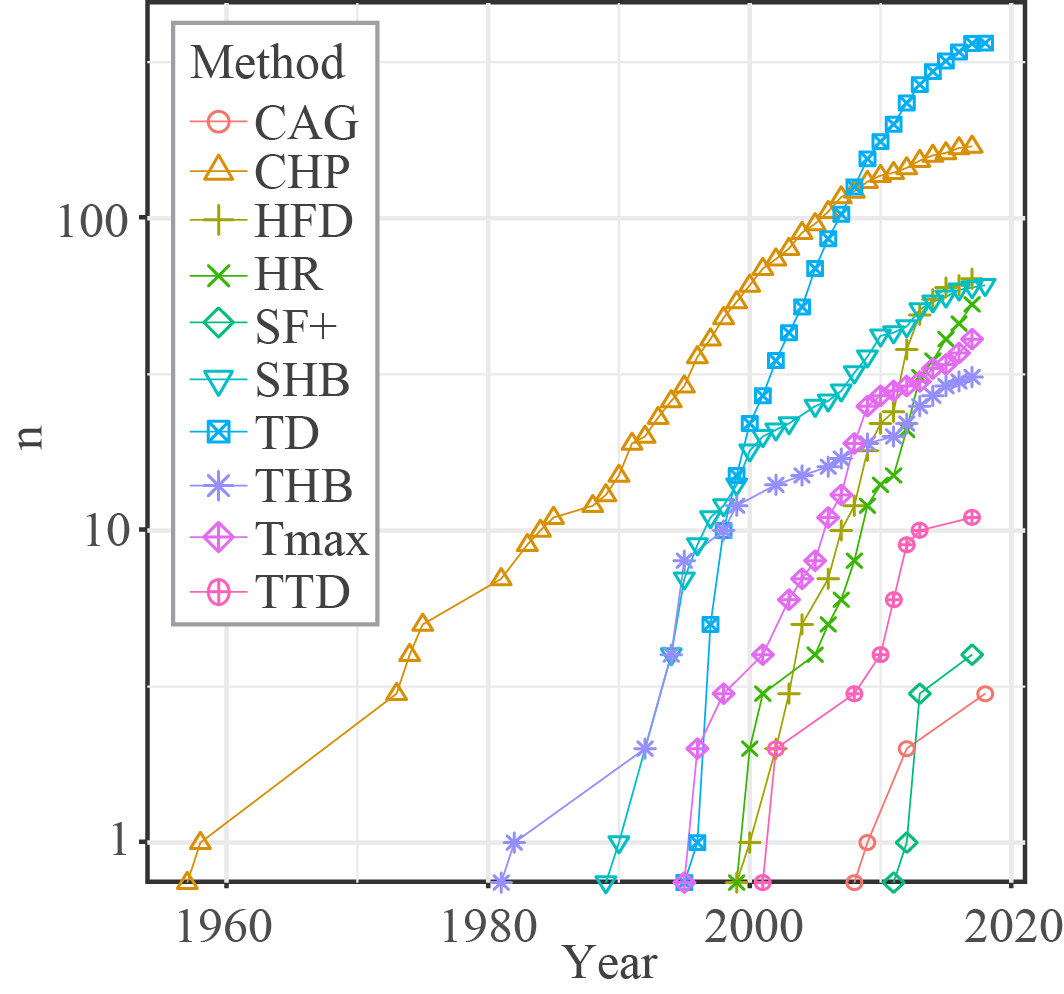
\includegraphics[width=0.8\linewidth]{figure/appendixA/fig1} 

}

\caption[Representation of the cumulative number of studies using different sap flow methods between 1957 and 2017]{Representation of the cumulative number of studies using different sap flow methods between 1957 and 2017 (adapted and updated from Poyatos et al. 2016). CAG: calibrated average gradient; CHP: compensation heat pulse (early heat pulse methods have been considered CHP, Edwards et al. 1997); HFD: head field deformation; HR: heat ratio, SF+: sapflow+; SHB: stem heat balance; TD: thermal dissipation; THB: trunk heat balance; Tmax: T-max heat pulse; TTD: transient thermal dissipation. Notice the logarithmic scale on the y-axis.}\label{fig:apa11}
\end{figure}
\setlength{\abovecaptionskip}{0pt} \newpage

\setlength{\abovecaptionskip}{15pt}
\begin{figure}[hbt!]

{\centering 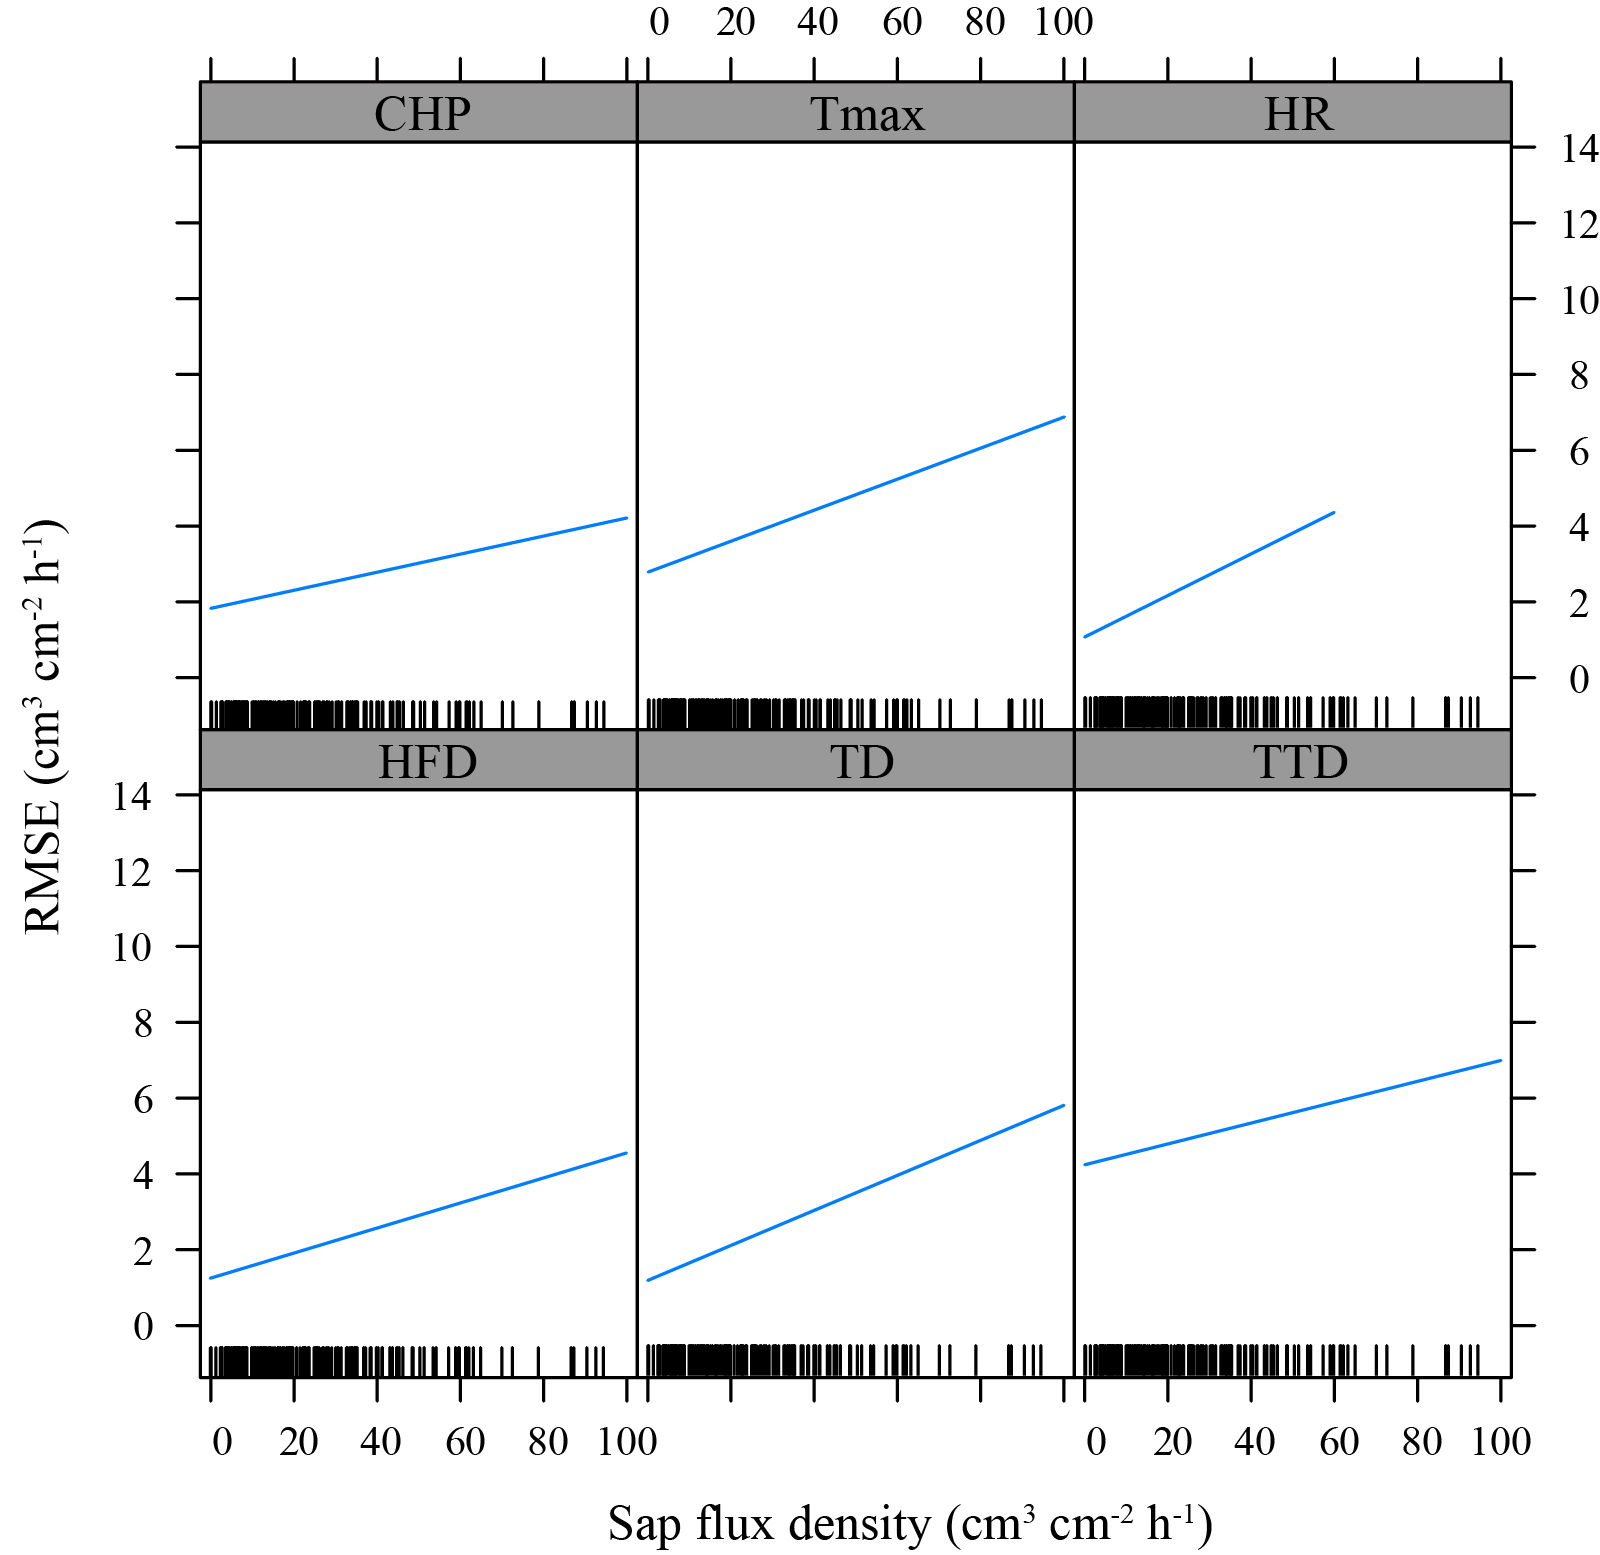
\includegraphics[width=1\linewidth]{figure/appendixA/fig2} 

}

\caption[Relationship between root mean square error (RMSE) and sap flux density.]{Relationship between root mean square error (RMSE) and sap flux density (mean calibration range) and for different sap flux density methods, as predicted by the LMM model presented in Table 3.}\label{fig:apa122}
\end{figure}
\setlength{\abovecaptionskip}{0pt}

\newpage
\begin{figure}[hbt!]

{\centering 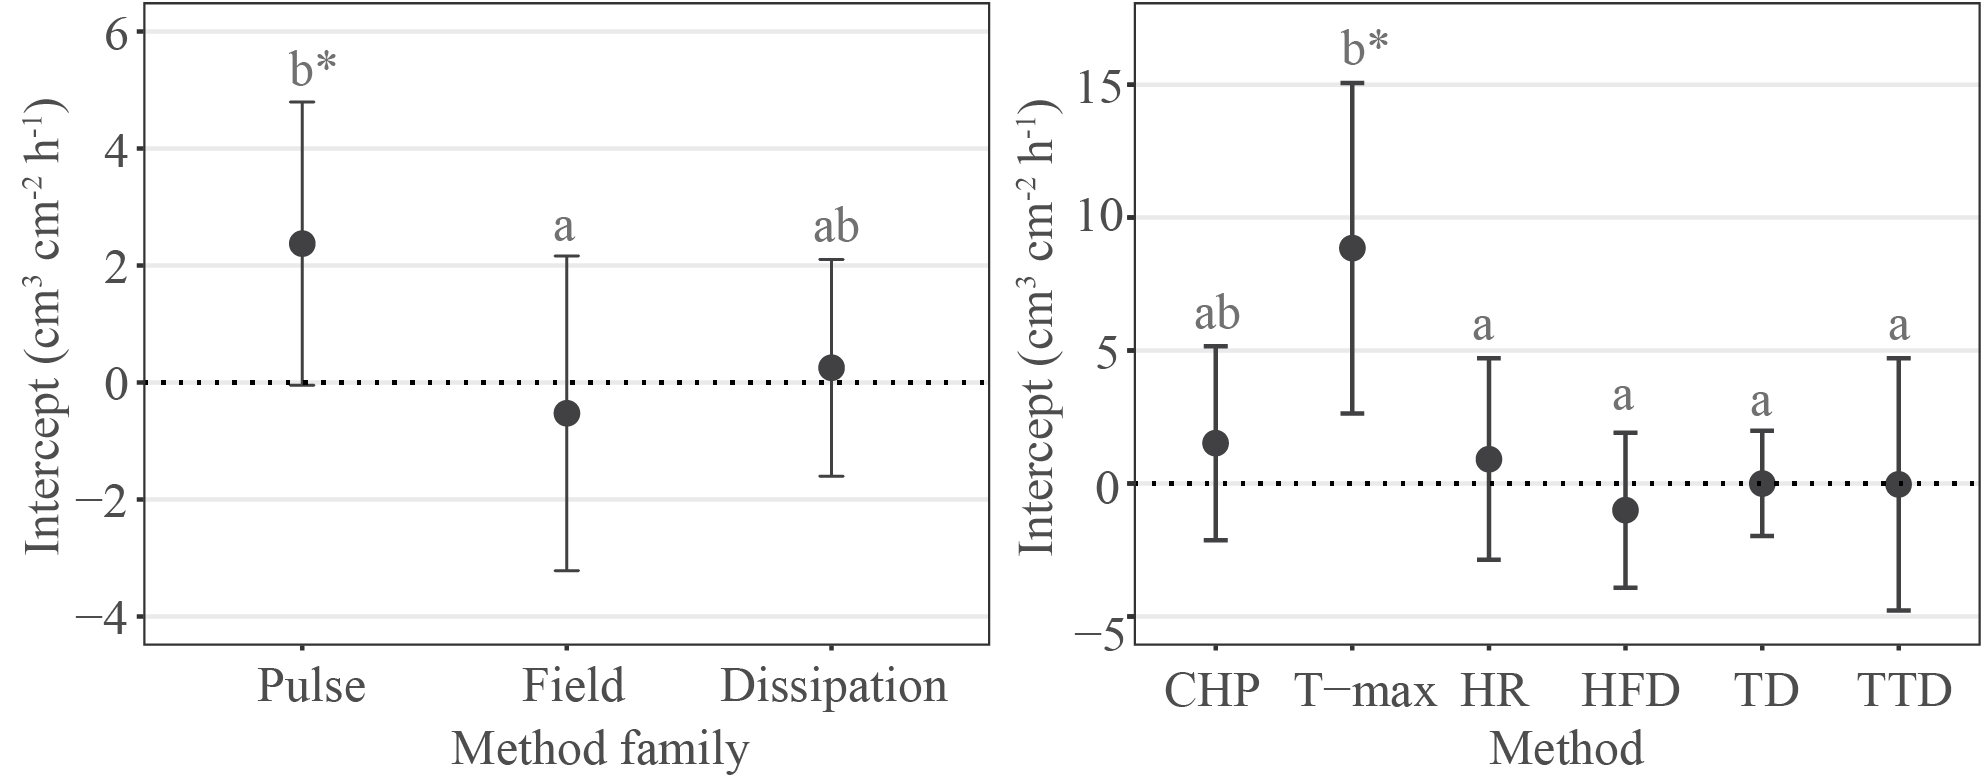
\includegraphics[width=1\linewidth]{figure/appendixA/fig3} 

}

\caption[Predictions of the LMM models calculated from least-squares means of the intercept ($\beta_{0}$) of the linear model.]{Predictions of the LMM models calculated from least-squares means of the intercept ($\beta_{0}$) of the linear model (Eq. 3). Different letters indicate significant differences between factors levels evaluated with Tukey’s test. Horizontal, dotted lines indicate reference, perfect calibration values for a given metric. Asterisks (*) indicate significant (p<0.05) departure from those reference values.}\label{fig:apa13}
\end{figure}\newpage
\section{Tables A}\label{tables-a}

\begingroup\fontsize{6}{8}\selectfont
\begin{longtable}[t]{>{\raggedright\arraybackslash}p{12em}>{\raggedright\arraybackslash}p{3em}l>{\raggedright\arraybackslash}p{6em}l>{\raggedleft\arraybackslash}p{3em}}
\caption[Summary table of the studies used in the analyses.]{\label{tab:unnamed-chunk-1}Summary table of the studies used in the analyses presented in the paper. Sap flow method, species, calibration material, porosity and average stem/tree diameter are reported.}\\
\toprule
Study & Method & Species & Calibration material & Wood porosity & Diameter (cm)\\
\midrule
\endfirsthead
\caption[]{\label{tab:unnamed-chunk-1}Summary table of the studies used in the analyses presented in the paper. Sap flow method, species, calibration material, porosity and average stem/tree diameter are reported. \textit{(continued)}}\\
\toprule
Study & Method & Species & Calibration material & Wood porosity & Diameter (cm)\\
\midrule
\endhead
\
\endfoot
\bottomrule
\endlastfoot
Alarcon $et\;\, al.$ 2005 & CHP & $Citrus\;\,limon$ & whole plant & Diffuse porous & 2.50\\
Ballester et al 2011 & CHP & $Citrus\;\,clementina$ & whole plant & Diffuse porous & \\
Barret $et\;\, al.$ 1995 & CHP & $Corymbia\;\,maculata$ & without roots & Diffuse porous & \\
Bleby $et\;\, al.$ 2004 & CHP & $Eucalyptus\;\,marginata$ & whole plant & Diffuse porous & 10.00\\
Bleby $et\;\, al.$ 2004 & HR & $Eucalyptus\;\,marginata$ & whole plant & Diffuse porous & 10.00\\
Braun and Schmid 1999 & TD & $Vitis\;\,vinifera$ & whole plant & Ring porous & 3.75\\
Burgess $et\;\, al.$ 2001 & HR & $Eucalyptus\;\,marginata$ & whole plant & Diffuse porous & \\
Bush $et\;\, al.$ 2010 & TD & $Populus\;\,fremontii$ & stem segment & Diffuse porous & 5.08\\
Bush $et\;\, al.$ 2010 & TD & $Tilia\;\,cordata$ & stem segment & Diffuse porous & 4.83\\
Cain 2009 & TD & $Macaranga\;\,hypoleuca$ & stem segment & Diffuse porous & 82.00\\
Cain 2009 & TD & $Macaranga\;\,pearsonii$ & stem segment & Diffuse porous & 67.00\\
Caspari $et\;\, al.$ 1993 & CHP & $Pyrus\;\,serotina$ & whole plant & Diffuse porous & 6.62\\
Caterina $et\;\, al.$ 2013 & TD & $Juniperus\;\,virginiana$ & stem segment & Tracheids & 8.00\\
Chan 2015 & TD & $Abies\;\,concolor$ & stem segment & Tracheids & 6.00\\
Cohen $et\;\, al.$ 1981 & T-max & $Platanus\;\,orientalis$ & stem segment & Diffuse porous & 6.70\\
Cohen $et\;\, al.$ 1981 & T-max & $Populus\;\,alba$ & stem segment & Diffuse porous & 6.70\\
Cohen $et\;\, al.$ 1998 & T-max & $Malus\;\,domestica$ & whole plant & Diffuse porous & \\
Dragoni $et\;\, al.$ 2005 & CHP & $Malus\;\,domestica$ & whole plant & Diffuse porous & 6.50\\
Dye $et\;\, al.$ 1996 & CHP & $Pinus\;\,patula$ & without roots & Tracheids & \\
Fernandez $et\;\, al.$ 1999 & CHP & $Olea\;\,europaea$ & stem segment & Diffuse porous & 8.80\\
Fernandez $et\;\, al.$ 1999 & CHP & $Olea\;\,europaea$ & without roots & Diffuse porous & \\
Fernandez $et\;\, al.$ 2006 & CHP & $Citrus\;\,sinensis$ & stem segment & Diffuse porous & 7.80\\
Fernandez $et\;\, al.$ 2006 & CHP & $Citrus\;\,sinensis$ & without roots & Diffuse porous & 10.40\\
Fernandez $et\;\, al.$ 2006 & CHP & $Olea\;\,europaea$ & stem segment & Diffuse porous & 8.20\\
Fernandez $et\;\, al.$ 2006 & CHP & $Olea\;\,europaea$ & without roots & Diffuse porous & 9.80\\
Fernandez $et\;\, al.$ 2006 & CHP & $Prunus\;\,domestica$ & stem segment & Diffuse porous & 8.00\\
Fernandez $et\;\, al.$ 2006 & CHP & $Prunus\;\,domestica$ & without roots & Diffuse porous & 7.00\\
Fuchs $et\;\, al.$ 2017 & HFD & $Acer\;\,pseudoplatanus$ & stem segment & Diffuse porous & 10.56\\
Fuchs $et\;\, al.$ 2017 & HFD & $Fagus\;\,sylvatica$ & stem segment & Diffuse porous & 9.42\\
Fuchs $et\;\, al.$ 2017 & HFD & $Tilia\;\,cordata$ & stem segment & Diffuse porous & 9.29\\
Fuchs $et\;\, al.$ 2017 & HR & $Acer\;\,pseudoplatanus$ & stem segment & Diffuse porous & \\
Fuchs $et\;\, al.$ 2017 & HR & $Fagus\;\,sylvatica$ & stem segment & Diffuse porous & \\
Fuchs $et\;\, al.$ 2017 & HR & $Tilia\;\,cordata$ & stem segment & Diffuse porous & \\
Fuchs $et\;\, al.$ 2017 & TD & $Acer\;\,campestre$ & stem segment & Diffuse porous & 11.81\\
Fuchs $et\;\, al.$ 2017 & TD & $Acer\;\,pseudoplatanus$ & stem segment & Diffuse porous & 10.80\\
Fuchs $et\;\, al.$ 2017 & TD & $Fagus\;\,sylvatica$ & stem segment & Diffuse porous & 9.83\\
Fuchs $et\;\, al.$ 2017 & TD & $Populus\;\,nigra$ & stem segment & Diffuse porous & 10.77\\
Fuchs $et\;\, al.$ 2017 & TD & $Tilia\;\,cordata$ & stem segment & Diffuse porous & 9.41\\
Gonzalez-Altozano $et\;\, al.$ 1998 & CHP & $Citrus\;\,reticulata$ & whole plant & Diffuse porous & 11.50\\
Gonzalez-Altozano $et\;\, al.$ 1998 & T-max & $Citrus\;\,reticulata$ & whole plant & Diffuse porous & 11.50\\
Granier 1985 & TD & $Pinus\;\,nigra$ & stem segment & Tracheids & 4.50\\
Granier 1985 & TD & $Pseudotzuga\;\,menziesii$ & stem segment & Tracheids & 4.50\\
Granier 1985 & TD & $Quercus\;\,pedunculata$ & stem segment & Ring porous & 4.50\\
Green $et\;\, al.$ 1988 & CHP & $Actinidia\;\,chinensis$ & stem segment & Diffuse porous & 5.25\\
Green $et\;\, al.$ 1988 & CHP & $Actinidia\;\,chinensis$ & whole plant & Diffuse porous & 5.40\\
Green $et\;\, al.$ 1988 & CHP & $Malus\;\,sylvestris$ & whole plant & Diffuse porous & 5.60\\
Gutierrez $et\;\, al.$ 1994 & SHB & $Acacia\;\,koa$ & whole plant & Diffuse porous & \\
Gutierrez $et\;\, al.$ 1994 & SHB & $Coffea\;\,arabica$ & whole plant & Diffuse porous & \\
Gutierrez Soto $et\;\, al.$ 2012 & HR & $Carica\;\,papaya$ & whole plant & Monocot & \\
Hatton $et\;\, al.$ 1995 & CHP & $Eucalyptus\;\,populnea$ & without roots & Diffuse porous & 5.40\\
Heilman $et\;\, al.$ 1990 & SHB & $Ligustrum\;\,japonicum$ & whole plant & Diffuse porous & 1.00\\
Herbs $et\;\, al.$ 2007 & TD & $Acer\;\,campestre$ & stem segment & Diffuse porous & \\
Herbs $et\;\, al.$ 2007 & TD & $Crataegus\;\,monogina$ & stem segment & Diffuse porous & \\
Hultine $et\;\, al.$ 2010 & TD & $Tamarix\;\,ramossisima$ & stem segment & Ring porous & 4.16\\
Intrigliolo $et\;\, al.$ 2009 & T-max & $Vitis\;\,vinifera$ & whole plant & Ring porous & \\
Isarangkool $et\;\, al.$ 2009 & TTD & $Abies\;\,concolor$ & stem segment & Diffuse porous & 5.14\\
Isarangkool $et\;\, al.$ 2009 & TTD & $Hevea\;\,brasiliensis$ & stem segment & Diffuse porous & 4.69\\
Isarangkool $et\;\, al.$ 2009 & TTD & $Mangifera\;\,indica$ & stem segment & Diffuse porous & 4.35\\
Johan Uddling $et\;\, al.$ 2009 & TD & $Betula\;\,papyrifera$ & stem segment & Diffuse porous & \\
Lu 2002 & TD & $Garcinia\;\,mangostana$ & whole plant & Diffuse porous & 4.00\\
Lu 2002 & TD & $Mangifera\;\,indica$ & whole plant & Diffuse porous & 2.30\\
Lu 2002 & TD & $Musa\;\,spp.$ & whole plant & Monocot & 12.00\\
Lu and Chacko 1998 & TD & $Mangifera\;\,indica$ & whole plant & Diffuse porous & 2.30\\
Madurapperuma $et\;\, al.$ 2009 & HR & $Syagrus\;\,romanzoffiana$ & whole plant & Monocot & \\
Michell $et\;\, al.$ 2009 & HR & $Eucalyptus\;\,capillosa$ & without roots & Diffuse porous & 6.50\\
Montague $et\;\, al.$ 2006 & TD & $Liquidambar\;\,styraciflua$ & whole plant & Diffuse porous & 5.30\\
Montague $et\;\, al.$ 2006 & TD & $Populus\;\,deltoides$ & whole plant & Diffuse porous & 5.60\\
Montague $et\;\, al.$ 2006 & TD & $Pyrus\;\,calleryana$ & whole plant & Diffuse porous & 6.60\\
Montague $et\;\, al.$ 2006 & TD & $Quercus\;\,robur\;\,x\;\,Q.\;\,Bicolor$ & whole plant & Ring porous & 5.70\\
Nadezhdina $et\;\, al.$ 1998 & HFD & $Tilia\;\,cordata$ & without roots & Diffuse porous & 12.00\\
Nortes $et\;\, al.$ 2009 & CHP & $Prunus\;\,dulcis$ & whole plant & Diffuse porous & 15.00\\
Paudel $et\;\, al.$ 2013 & TD & $Malus\;\,domestica$ & stem segment & Diffuse porous & 4.01\\
Paudel $et\;\, al.$ 2013 & TD & $Peltophorum\;\,dubium$ & stem segment & Diffuse porous & 3.70\\
Paudel $et\;\, al.$ 2013 & TD & $Prunus\;\,persica$ & stem segment & Diffuse porous & 4.00\\
Paudel $et\;\, al.$ 2013 & TTD & $Malus\;\,domestica$ & stem segment & Diffuse porous & 4.01\\
Paudel $et\;\, al.$ 2013 & TTD & $Peltophorum\;\,dubium$ & stem segment & Diffuse porous & 3.70\\
Paudel $et\;\, al.$ 2013 & TTD & $Prunus\;\,persica$ & stem segment & Diffuse porous & 4.00\\
Peters $et\;\, al.$ 2017 & TD & $Larix\;\,decidua$ & stem segment & Tracheids & 16.50\\
Peters $et\;\, al.$ 2017 & TD & $Picea\;\,abies$ & stem segment & Tracheids & 15.90\\
Prendergast $et\;\, al.$ 2007 & T-max & $Actinidia\;\,chinensis$ & stem segment & Diffuse porous & 9.50\\
Shackel $et\;\, al.$ 1992 & SHB & $Prunus\;\,persica$ & whole plant & Diffuse porous & 6.25\\
Smith $et\;\, al.$ 1995 & CHP & $Acacia\;\,holosericea$ & stem segment & Diffuse porous & \\
Smith $et\;\, al.$ 1995 & CHP & $Acacia\;\,holosericea$ & without roots & Diffuse porous & \\
Smith $et\;\, al.$ 1995 & CHP & $Acacia\;\,nilotica$ & stem segment & Diffuse porous & \\
Smith $et\;\, al.$ 1995 & CHP & $Azadirachta\;\,indica$ & stem segment & Diffuse porous & \\
Smith $et\;\, al.$ 1995 & CHP & $Azadirachta\;\,indica$ & without roots & Diffuse porous & \\
Sperling $et\;\, al.$ 2012 & TD & $Phoenix\;\,datylifera$ & whole plant & Monocot & 60.00\\
Steppe $et\;\, al.$ 2010 & CHP & $Fagus\;\,grandifolia$ & stem segment & Diffuse porous & 18.00\\
Steppe $et\;\, al.$ 2010 & HFD & $Fagus\;\,grandifolia$ & stem segment & Diffuse porous & 18.12\\
Steppe $et\;\, al.$ 2010 & TD & $Fagus\;\,grandifolia$ & stem segment & Diffuse porous & 18.00\\
Sun $et\;\, al.$ 2012 & TD & $Liquidambar\;\,styraciflua$ & without roots & Diffuse porous & 7.50\\
Sun $et\;\, al.$ 2012 & TD & $Pinus\;\,echinata$ & without roots & Tracheids & 7.50\\
Sun $et\;\, al.$ 2012 & TD & $Pinus\;\,taeda$ & without roots & Tracheids & 7.50\\
Sun $et\;\, al.$ 2012 & TD & $Populus\;\,deltoides$ & without roots & Diffuse porous & 7.50\\
Sun $et\;\, al.$ 2012 & TD & $Quercus\;\,alba$ & without roots & Ring porous & 7.50\\
Sun $et\;\, al.$ 2012 & TD & $Ulmus\;\,americana$ & without roots & Ring porous & 7.50\\
Swanson and Whitfield 1981 & CHP & $Nothofagus\;\,solandri$ & whole plant & Diffuse porous & 11.00\\
Swanson and Whitfield 1981 & CHP & $Pinus\;\,radiata$ & whole plant & Tracheids & 5.00\\
Urban $et\;\, al.$ 2012 & SHB & $Humulus\;\,lupulus$ & without roots & Ring porous & \\
Vellame $et\;\, al.$ 2010 & SHB & $Citrus\;\,sinensis$ & whole plant & Diffuse porous & 1.40\\*
\end{longtable}
\endgroup{}

\newpage
\begin{table}[!h]

\caption[Anova summary of the LMM models.]{\label{tab:unnamed-chunk-2}Anova summary of the LMM models, using the same structure as objective 1, comparing calibrations reported in SFD and SF units (Units) for CHP and TD. CM (Calibration material).}
\centering
\fontsize{6}{8}\selectfont
\begin{tabular}[t]{ccccccccc}
\toprule
Method & Calibration metric & Variable & Sum sq & Mean Sq & NumDF & DenDF & F.value & Pr(>F)\\
\midrule
 &  & Units & 0.09 & 0.09 & 1 & 52.05 & 1.09 & 0.302\\
\cmidrule{3-9}
 & \multirow[t]{-2}{*}{\centering\arraybackslash Ln-Ratio} & CM & 0.20 & 0.10 & 2 & 44.43 & 1.24 & 0.299\\
\cmidrule{2-9}
 &  & Units & 0.07 & 0.07 & 1 & 25.27 & 0.37 & 0.55\\
\cmidrule{3-9}
 & \multirow[t]{-2}{*}{\centering\arraybackslash Slope} & CM & 0.24 & 0.12 & 2 & 40.07 & 0.59 & 0.558\\
\cmidrule{2-9}
 &  & Units & 0.00 & 0.00 & 1 & 12.35 & 0.02 & 0.89\\
\cmidrule{3-9}
 & \multirow[t]{-2}{*}{\centering\arraybackslash Slope (ln-ln)} & CM & 0.14 & 0.07 & 2 & 22.13 & 0.91 & 0.416\\
\cmidrule{2-9}
 &  & Units & 1.07 & 1.07 & 1 & 20.77 & 4.30 & 0.051 .\\
\cmidrule{3-9}
\multirow[t]{-8}{*}{\centering\arraybackslash CHP} & \multirow[t]{-2}{*}{\centering\arraybackslash Z-Cor} & CM & 4.63 & 2.32 & 2 & 34.98 & 9.28 & 0.001 ***\\
\cmidrule{1-9}
 &  & Units & 0.05 & 0.05 & 1 & 26.72 & 0.41 & 0.529\\
\cmidrule{3-9}
 & \multirow[t]{-2}{*}{\centering\arraybackslash Ln-Ratio} & CM & 0.14 & 0.07 & 2 & 16.64 & 0.58 & 0.571\\
\cmidrule{2-9}
 &  & Units & 0.16 & 0.16 & 1 & 44.72 & 2.28 & 0.138\\
\cmidrule{3-9}
 & \multirow[t]{-2}{*}{\centering\arraybackslash Slope} & CM & 0.17 & 0.08 & 2 & 14.84 & 1.17 & 0.338\\
\cmidrule{2-9}
 &  & Units & 0.22 & 0.22 & 1 & 72.67 & 2.18 & 0.144\\
\cmidrule{3-9}
 & \multirow[t]{-2}{*}{\centering\arraybackslash Slope (ln-ln)} & CM & 0.14 & 0.07 & 2 & 29.27 & 0.71 & 0.501\\
\cmidrule{2-9}
 &  & Units & 0.08 & 0.08 & 1 & 26.07 & 0.28 & 0.598\\
\cmidrule{3-9}
\multirow[t]{-8}{*}{\centering\arraybackslash TD} & \multirow[t]{-2}{*}{\centering\arraybackslash Z-Cor} & CM & 0.02 & 0.01 & 2 & 17.41 & 0.03 & 0.969\\
\bottomrule
\end{tabular}
\end{table}
\newpage
\begin{landscape}
\begin{table}

\caption[Summary of the LMM models of Ln-Ratio (accuracy), Slope (proportional bias), Slope (ln-ln) (linearity) and Z-Cor (precision) as a function of Methods and Calibration material.]{\label{tab:unnamed-chunk-3}Summary of the LMM models of Ln-Ratio (accuracy), Slope (proportional bias), Slope (ln-ln) (linearity) and Z-Cor (precision) as a function of Methods and Calibration material (CM; Whole plant: whole plant on a container or lysimeter; No-roots: whole plant without roots). CHP is the reference level for the variable Method and Stem segment is the reference level for CM, corresponding to the model intercept. All other coefficient estimates indicate the difference relative to the intercept. $\sigma^{2}$ is the within-groups random variability (residuals of the model). $\tau_{00}$ is the between-group random variability. N is the number of levels within random groups. ICC is the Intraclass Correlation Coefficients of each random group. $R^{2}m$ and $R^{2}c$ are the variability explained by the fixed and the random factors, respectively.}
\centering
\resizebox{\linewidth}{!}{
\fontsize{5}{7}\selectfont
\begin{tabular}[t]{ccccccccccccc}
\toprule
Coefficients & Estimate & Conf. Int. & p-value & Estimate & Conf. Int. & p-value & Estimate & Conf. Int. & p-value & Estimate & Conf. Int. & p-value\\
\midrule
Fixed effects &  &  &  &  &  &  &  &  &  &  &  & \\
(Intercept) & 0.19 & -0.052\: , \:0.425 & 0.129 & 0.96 & 0.779\: , \:1.135 & <0.001 & 0.85 & 0.719\: , \:0.976 & <0.001 & 2.32 & 1.982\: , \:2.653 & 2.32\\
Method (T-max) & -0.19 & -0.611\: , \:0.240 & 0.395 & -0.27 & -0.584\: , \:0.038 & 0.089 & -0.08 & -0.312\: , \:0.142 & 0.463 & -0.08 & -0.669\: , \:0.506 & -0.08\\
Method (HR) & -0.28 & -0.510\: , \:-0.047 & 0.019 & -0.04 & -0.247\: , \:0.162 & 0.683 & 0.06 & -0.106\: , \:0.221 & 0.488 & 0.16 & -0.205\: , \:0.525 & 0.16\\
Method (HFD) & -0.21 & -0.409\: , \:-0.003 & 0.048 & 0.01 & -0.167\: , \:0.193 & 0.886 & 0.00 & -0.143\: , \:0.143 & 1 & 0.54 & 0.220\: , \:0.862 & 0.54\\
Method (SHB) & -0.37 & -0.843\: , \:0.095 & 0.124 & -0.04 & -0.365\: , \:0.285 & 0.809 & 0.18 & -0.058\: , \:0.427 & 0.139 & 0.45 & -0.170\: , \:1.070 & 0.45\\
Method (TD) & -0.65 & -0.847\: , \:-0.457 & <0.001 & -0.20 & -0.368\: , \:-0.041 & 0.015 & 0.28 & 0.160\: , \:0.406 & <0.001 & -0.12 & -0.423\: , \:0.173 & -0.12\\
Method (TTD) & -0.62 & -0.941\: , \:-0.310 & <0.001 & -0.22 & -0.503\: , \:0.066 & 0.134 & 0.20 & -0.016\: , \:0.421 & 0.072 & -0.37 & -0.877\: , \:0.133 & -0.37\\
CM (Whole plant) & -0.03 & -0.300\: , \:0.245 & 0.841 & -0.13 & -0.317\: , \:0.064 & 0.197 & -0.14 & -0.276\: , \:-0.003 & 0.05 & -0.67 & -1.034\: , \:-0.301 & -0.67\\
CM (No-roots) & -0.13 & -0.394\: , \:0.128 & 0.319 & -0.08 & -0.298\: , \:0.135 & 0.463 & -0.06 & -0.213\: , \:0.104 & 0.503 & -0.78 & -1.172\: , \:-0.379 & -0.78\\
Random effects &  &  &  &  &  &  &  &  &  &  &  & \\
$\sigma^{2}$ &  & 0.091 &  &  & 0.1 &  &  & 0.076 &  &  & 0.278 & \\
$\tau_{00}$ Species &  & 0.013 &  &  & 0.004 &  &  & 0.013 &  &  & 0.04 & \\
$\tau_{00}$ Study &  & 0.159 &  &  & 0.041 &  &  & 0.004 &  &  & 0.184 & \\
$N_{Species}$ &  & 65 &  &  & 65 &  &  & 65 &  &  & 65 & \\
$N_{Study}$ &  & 48 &  &  & 48 &  &  & 48 &  &  & 48 & \\
$ICC_{Species}$ &  & 0.049 &  &  & 0.029 &  &  & 0.137 &  &  & 0.08 & \\
$ICC_{Study}$ &  & 0.604 &  &  & 0.284 &  &  & 0.048 &  &  & 0.366 & \\
Observations &  & 290 &  &  & 290 &  &  & 290 &  &  & 290 & \\
\bottomrule
\end{tabular}}
\end{table}
\end{landscape}
\newpage

\chapter{Appendix Chapter 3}\label{appendix-chapter-3}

\newpage

\section{Figures B}\label{figures-b}

\setlength{\abovecaptionskip}{15pt}
\begin{figure}

{\centering 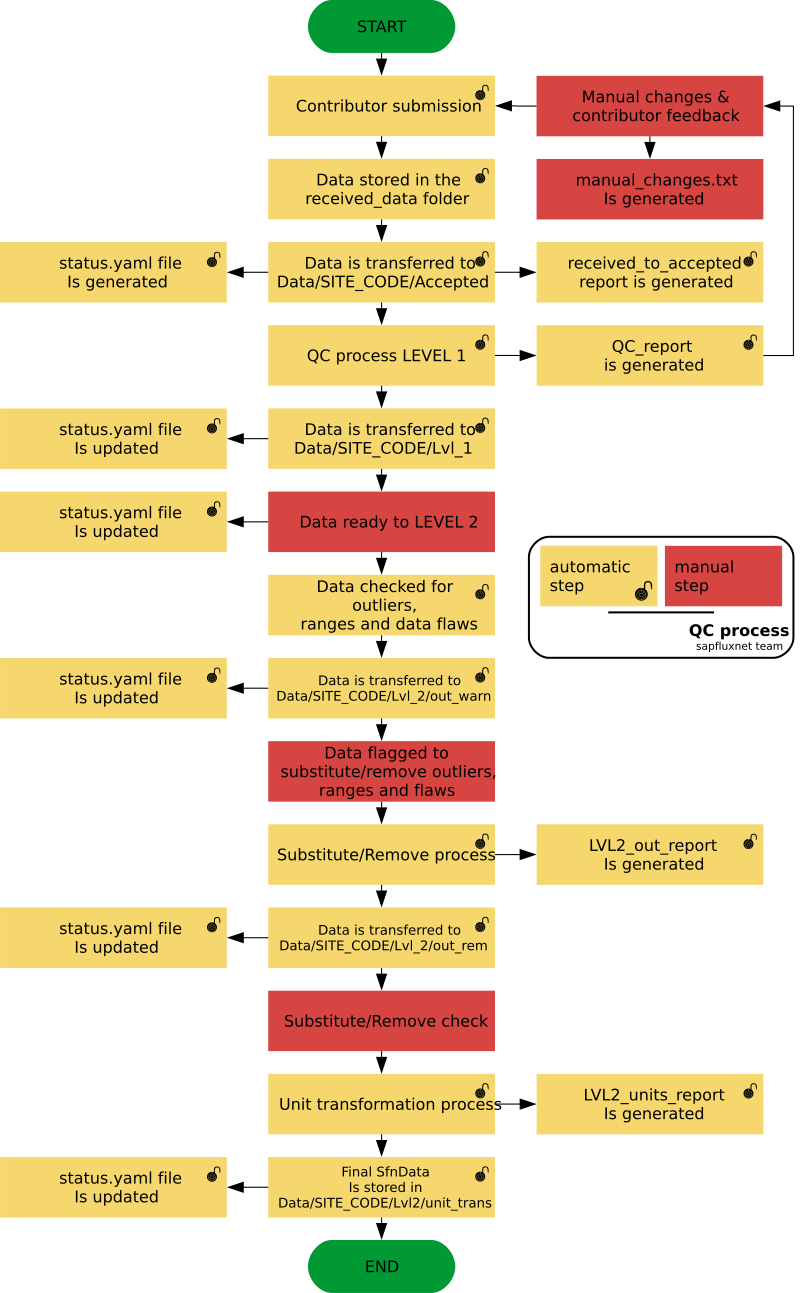
\includegraphics[width=0.8\linewidth]{figure/appendixB/QCsummary2} 

}

\caption[Overview of the data QC process.]{Overview of the data QC process, showing file management and identifying automatic (in yellow) and manual steps (in red).  The column on the left shows the different updates of the status file for each dataset and the column on the right shows generated data reports and steps requiring feedback or manual changes.}\label{fig:unnamed-chunk-5}
\end{figure}
\setlength{\abovecaptionskip}{0pt} \newpage

\setlength{\abovecaptionskip}{15pt}
\begin{figure}

{\centering 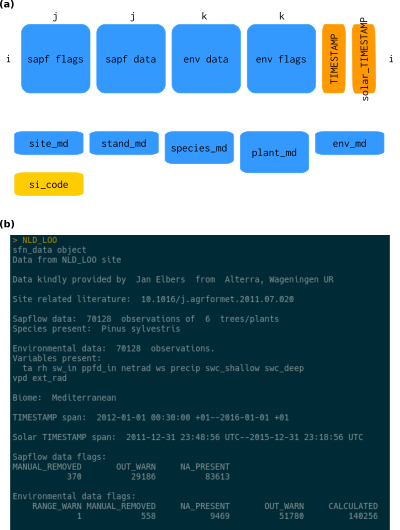
\includegraphics[width=0.7\linewidth]{figure/appendixB/schematics} 

}

\caption[Structure of sfn\_data objects.]{(a) Structure of sfn\_data objects, which are based on the S4 class. Boxes in the figure represent different slots where data are stored. Each object is identified by the 'si\_code', stored as a slot in the object, with the format of a character vector. Slots storing time series of data and the associated data flags are of class 'tibble' and have all the same number of rows (\textit{i}), corresponding to the the number of timesteps in the dataset and labelled with two POSIXct timestamp vectors TIMESTAMP, solar\_TIMESTAMP).The slot storing sap flow data, 'sapf\_data' contains(\textit{j}) columns and environmental data ('env\_data') contains \textit{k} columns, corresponding to the number of environmental variables present. Slots with the suffix 'md' refer to the different metadata and all are objects of class 'tibble' with different dimensions. For example, the number of rows in plant\_md' depends on the number of plants in the dataset (and this is depicted by the different length of the box). More information on the 'sfn\_data' class objects can be found in the vignette 'sfn-data-classes' of the package \textit{sapfluxnetr} (Granda et al. 2020). (b) Summary of an sfn\_data object, showing highlights of site metadata, data dimensions, timestamp span and flags present on the data.}\label{fig:unnamed-chunk-6}
\end{figure}
\setlength{\abovecaptionskip}{0pt} \newpage

\setlength{\abovecaptionskip}{15pt}
\begin{figure}

{\centering 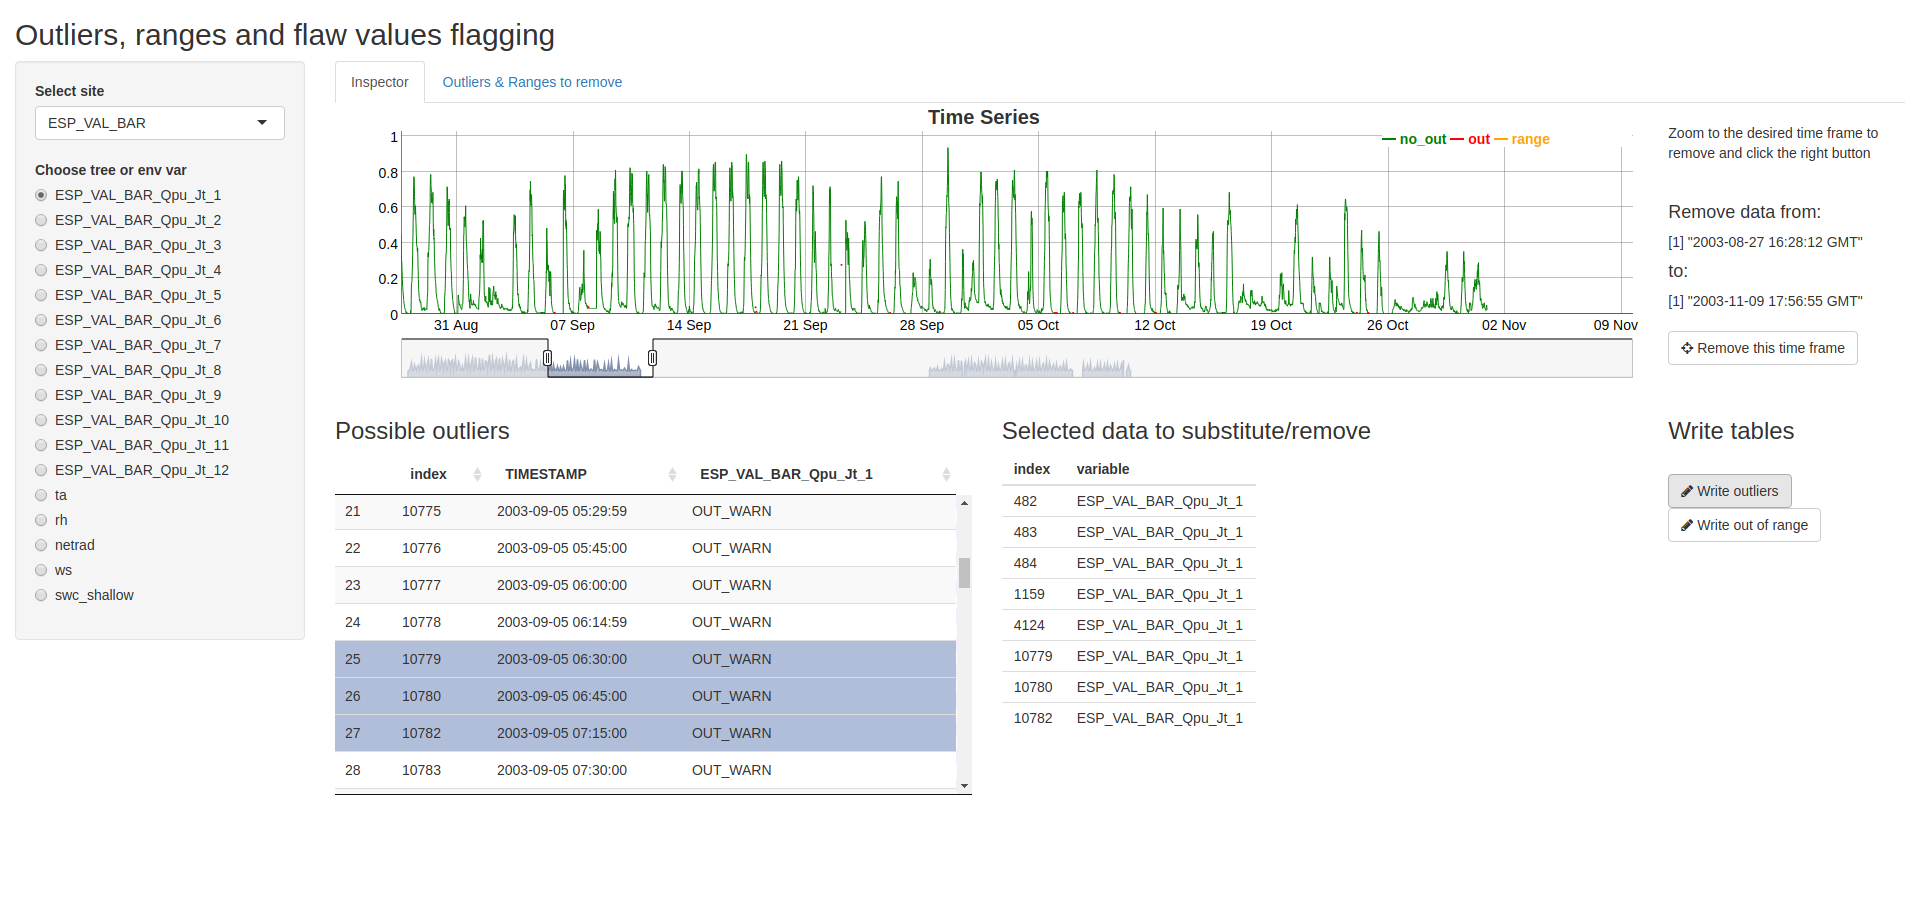
\includegraphics[width=1\linewidth]{figure/appendixB/outapp} 

}

\caption[Example screenshot of the app used for handling outliers and out of range values in time series.]{Example screenshot of the app used for handling outliers and out of range values in time series. The left column shows dataset and variable selection. The central part shows the time series, with out of range values in red and possible outliers in yellow. Rows to replace or remove are selected in a table and written to a text file when done.}\label{fig:unnamed-chunk-7}
\end{figure}
\setlength{\abovecaptionskip}{0pt} \newpage

\setlength{\abovecaptionskip}{15pt}
\begin{figure}
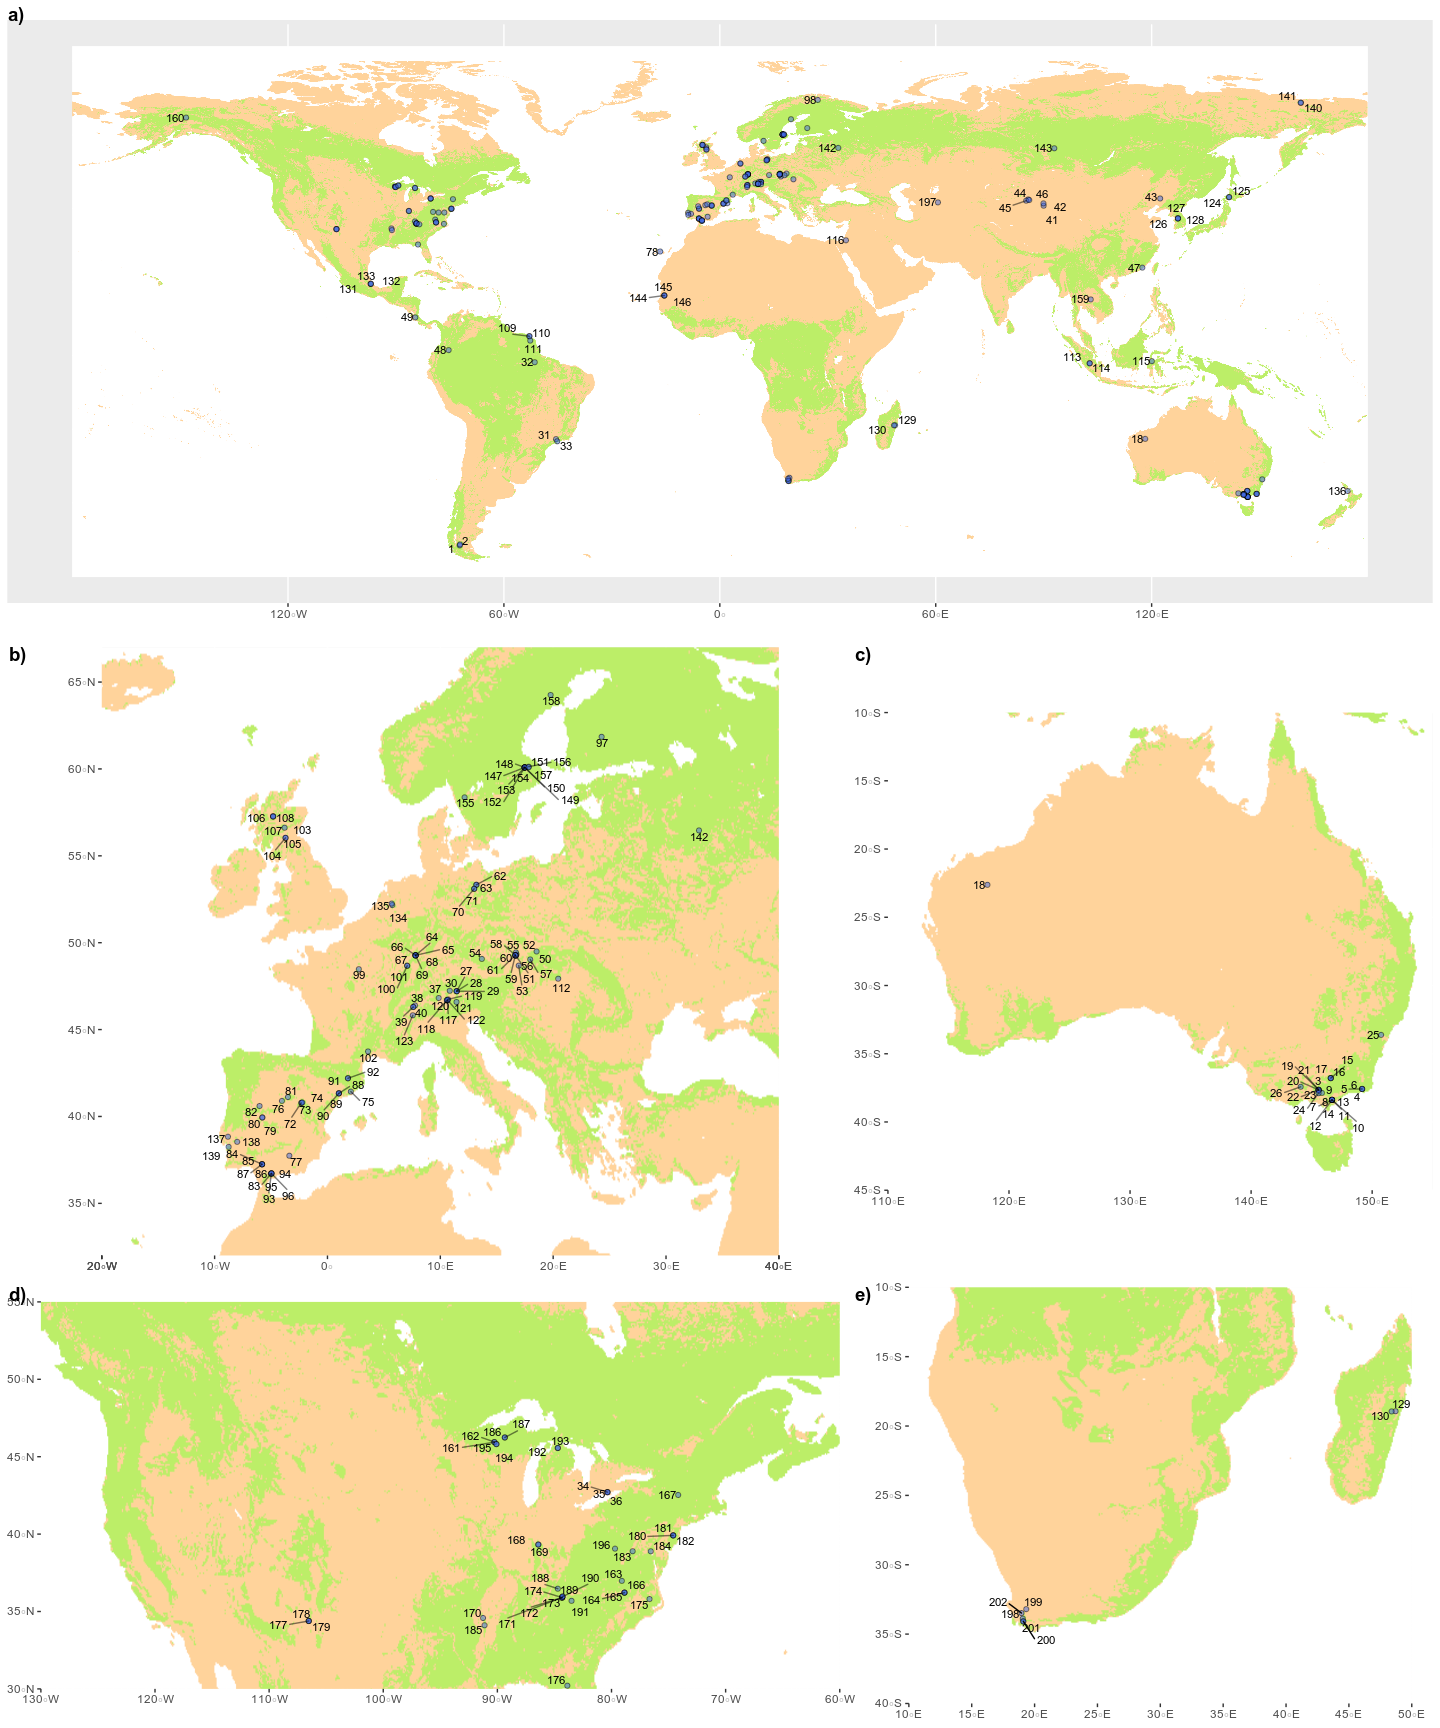
\includegraphics[width=1\linewidth]{figure/appendixB/regionalmaps} \caption[Detailed geographic distribution of SAPFLUXNET datasets]{Detailed geographic distribution of SAPFLUXNET datasets. Datasets are labelled by dataset number in Table S4. Woodland area from Crowther et al. (2015) shown in green.}\label{fig:regionalmaps}
\end{figure}
\setlength{\abovecaptionskip}{0pt}

\section{Tables B}\label{tables-b}
\begin{table}[H]

\caption[Data checks implemented in the first level of data quality control (QC1).]{\label{tab:tableQC1}Data checks implemented in the first level of data quality control (QC1).}
\centering
\resizebox{\linewidth}{!}{
\begin{tabular}[t]{c>{\centering\arraybackslash}p{20em}}
\toprule
Check & Description\\
\midrule
Metadata variables & All metadata variables are checked for presence and expected class (numeric, character, logical…).\\
Character variables values & All metadata character variables are checked against the possible values (factor levels) for that variable, raising a warning if some value is out of the expected.\\
E-mail check & E-mail provided by contributors is checked for validity\\
Coordinates and biome & Site coordinates are checked for correctness (are they inside the specified country?) and fixed if needed and possible. MAT and MAP values are obtained for that coordinates and the biome is calculated from that values.\\
Soil texture & Percentages of soil textures are used to calculate the USDA classification category if possible.\\
Species names & Species names in plant and species metadata are checked for spelling errors and the concordance between both metadata is also checked\\
Plant treatments & Check for uniformity in the treatment declared by plant.\\
Environmental variables presence & Check for concordance between the declared variables in the environmental metadata and the environmental data.\\
Timestamp & Format, NA presence (there is data, but there is no timestamp), concordance and continuity are checked.\\
Gap presence: & Data gaps (There is TIMESTAMP but there is no data) are summarised and visualized.\\
Soil water content & Check for percentage swc values and transform them to cm3/cm3\\
\bottomrule
\end{tabular}}
\end{table}
\newpage
\begin{table}[H]

\caption[Description of site metadata variables.]{\label{tab:tabsitemd}Description of site metadata variables.}
\centering
\resizebox{\linewidth}{!}{
\begin{tabular}[t]{c>{\centering\arraybackslash}p{20em}c>{\centering\arraybackslash}p{8em}}
\toprule
Variable & Description & Type & Units\\
\midrule
si\_name & Site name given by contributors & Character & None\\
si\_country & Country code (ISO) & Character & Fixed values\\
si\_contact\_firstname & Contributor first name & Character & None\\
si\_contact\_lastname & Contributor last name & Character & None\\
si\_contact\_email & Contributor email & Character & None\\
si\_contact\_institution & Contributor affiliation & Character & None\\
si\_addcontr\_firstname & Additional contributor first name & Character & None\\
si\_addcontr\_lastname & Additional contributor last name & Character & None\\
si\_addcontr\_email & Additional contributor email & Character & None\\
si\_addcontr\_institution & Additional contributor affiliation & Character & None\\
si\_lat & Site latitude (i.e. 42.36) & Numeric & Latitude, decimal format (WGS84)\\
si\_long & Site longitude (i.e. -8.23) & Numeric & Longitude, decimal format (WGS84)\\
si\_elev & Elevation above sea level & Numeric & meters\\
si\_paper & Paper with relevant information to understand the site as DOI links or DOI codes & Character & DOI link\\
si\_dist\_mgmt & Recent and historic disturbance and management events that affected the measurement years & Character & Fixed values\\
si\_igbp & Vegetation type based on IGBP classification & Character & Fixed values\\
si\_flux\_network & Logical indicating if site is participating in the FLUXNET network & Logical & Fixed values\\
si\_dendro\_network & Logical indicating if site is participating in the DENDROGLOBAL network & Logical & Fixed values\\
si\_remarks & Remarks and commentaries useful to grasp some site-specific peculiarities & Character & None\\
si\_code & sapfluxnet site code, unique for each site & Character & Fixed value\\
si\_mat & Site annual mean temperature, as obtained from WorldClim & Numeric & Celsius degrees\\
si\_map & Site annual mean precipitation, as obtained from WorldClim & Numeric & mm\\
si\_biome & Biome classification as per Whittaker diagram, based on mat and map obtained from WorldClim & Character & sapfluxnet calculated\\
\bottomrule
\end{tabular}}
\end{table}\newpage
\begin{table}[H]

\caption[Description of site metadata variables.]{\label{tab:tabstandmd}Description of site metadata variables.}
\centering
\resizebox{\linewidth}{!}{
\begin{tabular}[t]{c>{\centering\arraybackslash}p{20em}cc}
\toprule
Variable & Description & Type & Units\\
\midrule
st\_name & Stand name given by contributors & Character & None\\
st\_growth\_condition & Growth condition with respect to stand origin and management & Character & Fixed values\\
st\_treatment & Treatment applied at stand level & Character & None\\
st\_age & Mean stand age at the moment of sap flow measurements & Numeric & years\\
st\_height & Canopy height & Numeric & meters\\
st\_density & Total stem density for stand & Numeric & stems $\text{ha}^-1$\\
st\_basal\_area & Total stand basal area & Numeric & $\text{m}^2$ $\text{ha}^{-1}$\\
st\_lai & Total maximum stand leaf area (one-sided, projected) & Numeric & $\text{m}^2$ $\text{m}^{-2}$\\
st\_aspect & Aspect the stand is facing (exposure) & Character & Fixed values\\
st\_terrain & Slope and/or relief of the stand & Character & Fixed values\\
st\_soil\_depth & Soil total depth & Numeric & cm\\
st\_soil\_texture & Soil texture class, based on simplified USDA classification & Character & Fixed values\\
st\_sand\_perc & Soil sand content, \% mass & Numeric & \% percentage\\
st\_silt\_perc & Soil silt content, \% mass & Numeric & \% percentage\\
st\_clay\_perc & Soil clay content, \% mass & Numeric & \% percentage\\
st\_remarks & Remarks and commentaries useful to grasp some stand-specific peculiarities & Character & None\\
st\_USDA\_soil\_texture & USDA soil classification based on the percentages provided by the contributor & Character & sapfluxnet calculated\\
\bottomrule
\end{tabular}}
\end{table}\newpage
\begin{table}[H]

\caption[Description of species metadata variables.]{\label{tab:tabspeciesmd}Description of species metadata variables.}
\centering
\resizebox{\linewidth}{!}{
\begin{tabular}[t]{c>{\centering\arraybackslash}p{20em}c>{\centering\arraybackslash}p{20em}}
\toprule
Variable & Description & Type & Units\\
\midrule
sp\_name & Identity of each measured species & Character & Scientific name without author abbreviation, as accepted by The Plant List\\
sp\_ntrees & Number of trees measured of each species & Numeric & number of trees\\
sp\_leaf\_habit & Leaf habit of the measured species & Character & Fixed values\\
sp\_basal\_area\_perc & Basal area occupied by each measured species, in percentage over total stand basal area & Numeric & \% percentage\\
\bottomrule
\end{tabular}}
\end{table}
\begin{table}[H]

\caption[Description of plant metadata variables.]{\label{tab:tabplantmd}Description of plant metadata variables.}
\centering
\resizebox{\linewidth}{!}{
\begin{tabular}[t]{c>{\centering\arraybackslash}p{20em}c>{\centering\arraybackslash}p{12em}}
\toprule
Variable & Description & Type & Units\\
\midrule
pl\_name & Plant code assigned by contributors & Character & None\\
pl\_species & Species identity of the measured plant & Character & Scientific name without author abbreviation, as accepted by The Plant List\\
pl\_treatment & Experimental treatment (if any) & Character & None\\
pl\_dbh & Diameter at breast height of measured plants & Numeric & cm\\
pl\_height & Height of measured plants & Numeric & m\\
pl\_age & Plant age at the moment of measure & Numeric & years\\
pl\_social & Plant social status & Character & Fixed values\\
pl\_sapw\_area & Cross-sectional sapwood area & Numeric & $\text{cm}^2$\\
pl\_sapw\_depth & Sapwood depth, measured at breast height & Numeric & cm\\
pl\_bark\_thick & Plant bark thickness & Numeric & mm\\
pl\_leaf\_area & Leaf area of eachvvmeasured plant & Numeric & $\text{m}^2$\\
pl\_sens\_meth & Sap flow measures method & Character & Fixed values\\
pl\_sens\_man & Sap flow measures sensor manufacturer & Character & Fixed values\\
pl\_sens\_cor\_grad & Correction for natural temperature gradients method & Character & Fixed values\\
pl\_sens\_cor\_zero & Zero flow determination method & Character & Fixed values\\
pl\_sens\_calib & Was species-specific calibration used? & Logical & Fixed values\\
pl\_sap\_units & Uniformized sapfluxnet units for sapwood, leaf and plant level & Character & Fixed values\\
pl\_sap\_units\_orig & Original contribution units (at sapwood or plant level) & Character & Fixed values\\
pl\_sens\_length & Length of the needles or electrodes forming the sensor & Numeric & mm\\
pl\_sens\_hgt & Sensor installation height, measured from the ground & Numeric & m\\
pl\_sens\_timestep & Subdaily time step of sensor measures & Numeric & minutes\\
pl\_radial\_int &  & Character & Fixed values\\
pl\_azimut\_int &  & Character & Fixed values\\
pl\_remarks & Remarks and commentaries useful to grasp some plant-specific peculiarities & Character & None\\
pl\_code & sapfluxnet plant code, unique for each plant & Character & Fixed value\\
\bottomrule
\end{tabular}}
\end{table}\newpage
\begin{table}[H]

\caption[Description of environmental metadata variables.]{\label{tab:tabenvmd}Description of environmental metadata variables.}
\centering
\resizebox{\linewidth}{!}{
\begin{tabular}[t]{c>{\centering\arraybackslash}p{20em}cc}
\toprule
Variable & Description & Type & Units\\
\midrule
env\_time\_zone & Time zone of site used in the TIMESTAMPS & Character & Fixed values\\
env\_time\_daylight & Is daylight saving time applied to the original timestamp? & Logical & Fixed values\\
env\_timestep & Subdaily timestep of environmental measures & Numeric & minutes\\
env\_ta & Location of air temperature sensor & Character & Fixed values\\
env\_rh & Location of relative humidity sensor & Character & Fixed values\\
env\_vpd & Location of relative vapour pressure decifit sensor & Character & Fixed values\\
env\_sw\_in & Location of shortwave incoming radiation sensor & Character & Fixed values\\
env\_ppfd\_in & Location of incoming photosynthetic photon flux density sensor & Character & Fixed values\\
env\_netrad & Location of net radiation sensor & Character & Fixed values\\
env\_ws & Location of wind speed sensor & Character & Fixed values\\
env\_precip & Location of precipitation sensor & Character & Fixed values\\
env\_swc\_shallow\_depth & Average depth for shallow soil water content measures & Numeric & cm\\
env\_swc\_deep\_depth & Average depth for deep soil water content measures & Numeric & cm\\
env\_plant\_watpot & Availability of water potential values for the same measured plants during the sap flow measurements period & Character & Fixed values\\
env\_leafarea\_seasonal & Availability of seasonal course leaf area data and level & Character & Fixed values\\
env\_remarks & Remarks and commentaries useful to grasp some environmental-specific peculiarities & Character & None\\
\bottomrule
\end{tabular}}
\end{table}\newpage
\begin{table}[H]

\caption[Data checks implemented in the second level of data quality control (QC2).]{\label{tab:tableQC2}Data checks implemented in the second level of data quality control (QC2).}
\centering
\resizebox{\linewidth}{!}{
\begin{tabular}[t]{c>{\centering\arraybackslash}p{20em}}
\toprule
Data check & Description\\
\midrule
Sap flow units harmonisation & Sap flow expressed in $\text{cm}^3$ $\text{h}^{-1}$, sap flow per unit leaf\/sapwood area in $\text{cm}^3$ $\text{cm}^{-2}$ $\text{h}^{-1}$\\
Out of range detection & Out of range values are flagged automatically, examined in a visual app and removed if confirmed\\
Outlier detection & Outliers are flagged automatically, examined in a visual app and removed if confirmed\\
Radiation transformations & Interconversion between global radiation (sw\_in) and photosynthetically active radiation (ppfd\_in)\\
VPD and relative humidity & Interconversion between VPD and relative humidity\\
Extraterrestrial radiation and solar timestamp & Calculation of extraterrestrial radiation and solar timestamp from timestamp and geographical data\\
Sap flow interconversions & When sapwood or leaf areas were available, interconversions were applied between the different expression levels for sap flow (per plant, per sapwood area or per leaf area)\\
\bottomrule
\end{tabular}}
\end{table}\newpage
\begingroup\fontsize{7}{9}\selectfont
\begin{longtable}[t]{l>{\centering\arraybackslash}p{12em}cccc}
\caption[Datasets in the SAPFLUXNET database identified by numeric code, dataset code and site name.]{\label{tab:tabsites}Datasets in the SAPFLUXNET database identified by numeric code, dataset code and site name. Number of species per dataset, geographic coordinates and elevation are also shown. Negative coordinate values are shown for Southern and Western Hemispheres.}\\
\toprule
si\_code & si\_name & si\_lat & si\_long & si\_elev & \# species\\
\midrule
\endfirsthead
\caption[]{\label{tab:tabsites}Datasets in the SAPFLUXNET database identified by numeric code, dataset code and site name. Number of species per dataset, geographic coordinates and elevation are also shown. Negative coordinate values are shown for Southern and Western Hemispheres. \textit{(continued)}}\\
\toprule
si\_code & si\_name & si\_lat & si\_long & si\_elev & \# species\\
\midrule
\endhead
\
\endfoot
\bottomrule
\endlastfoot
ARG\_MAZ & Mazaruca\_Patagonia & -51.58 & -72.29 & 550 & 1\\
ARG\_TRE & Tres Marias & -51.32 & -72.19 & 460 & 1\\
AUS\_BRI\_BRI & Britannia Creek & -37.87 & 145.85 & 707 & 1\\
AUS\_CAN\_ST1\_EUC & Cann River & -37.58 & 149.17 & 180 & 1\\
AUS\_CAN\_ST2\_MIX & Cann River & -37.58 & 149.17 & 180 & 2\\
AUS\_CAN\_ST3\_ACA & Cann River & -37.58 & 149.17 & 180 & 1\\
AUS\_CAR\_THI\_00F & Carrajung & -38.38 & 146.68 & 610 & 1\\
AUS\_CAR\_THI\_0P0 & Carrajung & -38.38 & 146.68 & 610 & 1\\
AUS\_CAR\_THI\_0PF & Carrajung & -38.38 & 146.68 & 610 & 1\\
AUS\_CAR\_THI\_CON & Carrajung & -38.38 & 146.68 & 610 & 1\\
AUS\_CAR\_THI\_T00 & Carrajung & -38.38 & 146.68 & 610 & 1\\
AUS\_CAR\_THI\_T0F & Carrajung & -38.38 & 146.68 & 610 & 1\\
AUS\_CAR\_THI\_TP0 & Carrajung & -38.38 & 146.68 & 610 & 1\\
AUS\_CAR\_THI\_TPF & Carrajung & -38.38 & 146.68 & 610 & 1\\
AUS\_ELL\_HB\_HIG & Ella & -36.78 & 146.58 & 705 & 2\\
AUS\_ELL\_MB\_MOD & Ella & -36.78 & 146.58 & 693 & 1\\
AUS\_ELL\_UNB & Ella & -36.78 & 146.58 & 737 & 1\\
AUS\_KAR & Karijini NP & -22.62 & 118.22 & 710 & 1\\
AUS\_MAR\_HSD\_HIG & Maroondah & -37.64 & 145.58 & 468 & 2\\
AUS\_MAR\_HSW\_HIG & Maroondah & -37.65 & 145.57 & 297 & 2\\
AUS\_MAR\_MSD\_MOD & Maroondah & -37.64 & 145.58 & 467 & 2\\
AUS\_MAR\_MSW\_MOD & Maroondah & -37.65 & 145.57 & 261 & 2\\
AUS\_MAR\_UBD & Maroondah & -37.69 & 145.56 & 303 & 3\\
AUS\_MAR\_UBW & Maroondah & -37.89 & 145.57 & 336 & 3\\
AUS\_RIC\_EUC\_ELE & Richmond NSW EucFACE & -33.62 & 150.74 & 23 & 1\\
AUS\_WOM & WombatStateForest & -37.42 & 144.09 & 705 & 2\\
AUT\_PAT\_FOR & Patscherkofel & 47.21 & 11.45 & 1950 & 1\\
AUT\_PAT\_KRU & Patscherkofel & 47.21 & 11.45 & 2180 & 1\\
AUT\_PAT\_TRE & Patscherkofel & 47.21 & 11.45 & 2110 & 1\\
AUT\_TSC & Tschirgant south & 47.23 & 10.84 & 750 & 1\\
BRA\_CAM & Campos do Jordão & -22.69 & -45.52 & 2000 & 1\\
BRA\_CAX\_CON & Caxiuana & -1.79 & -51.43 & 15 & 8\\
BRA\_SAN & Santa Virgínia (PESM) & -23.28 & -45.18 & 1000 & 4\\
CAN\_TUR\_P39\_POS & TUR & 42.71 & -80.36 & 184 & 1\\
CAN\_TUR\_P39\_PRE & TUR & 42.71 & -80.36 & 184 & 1\\
CAN\_TUR\_P74 & TUR & 42.71 & -80.35 & 184 & 1\\
CHE\_DAV\_SEE & Davos & 46.82 & 9.86 & 1650 & 1\\
CHE\_LOT\_NOR & Lotschental & 46.39 & 7.76 & 1300 & 2\\
CHE\_PFY\_CON & Pfynwald & 46.30 & 7.60 & 615 & 1\\
CHE\_PFY\_IRR & Pfynwald & 46.30 & 7.60 & 615 & 1\\
CHN\_ARG\_GWD & Arghan & 40.75 & 89.99 & 830 & 1\\
CHN\_ARG\_GWS & Arghan & 41.38 & 89.94 & 830 & 1\\
CHN\_HOR\_AFF & Horqin & 42.72 & 122.37 & 226 & 1\\
CHN\_YIN\_ST1 & Yingbazar & 42.45 & 85.72 & 900 & 1\\
CHN\_YIN\_ST2\_DRO & Yingbazar & 42.11 & 85.13 & 930 & 1\\
CHN\_YIN\_ST3\_DRO & Yingbazar & 42.29 & 85.99 & 930 & 1\\
CHN\_YUN\_YUN & Yunxiao & 23.92 & 117.42 & 0 & 2\\
COL\_MAC\_SAF\_RAD & Macagual Universidad de la Amazonia & 1.50 & -75.36 & 360 & 1\\
CRI\_TAM\_TOW & TAMU Soltis Center & 10.39 & -84.63 & 600 & 17\\
CZE\_BIK & Bik & 49.49 & 18.53 & 875 & 1\\
CZE\_BIL\_BIL & Bilovice & 49.25 & 16.69 & 320 & 1\\
CZE\_KRT\_KRT & Krtiny & 49.32 & 16.75 & 480 & 1\\
CZE\_LAN & Lanžhot & 48.68 & 16.95 & 150 & 3\\
CZE\_LIZ\_LES & Liz & 49.07 & 13.68 & 858 & 1\\
CZE\_RAJ\_RAJ & Rajec & 49.44 & 16.70 & 600 & 1\\
CZE\_SOB\_SOB & Sobesice & 49.25 & 16.69 & 320 & 1\\
CZE\_STI & Stitna nad Vlari & 49.04 & 17.97 & 550 & 1\\
CZE\_UTE\_BEE & Utechov & 49.28 & 16.65 & 420 & 1\\
CZE\_UTE\_BNA & Utechov & 49.28 & 16.65 & 390 & 1\\
CZE\_UTE\_BPO & Utechov & 49.28 & 16.65 & 370 & 1\\
CZE\_UTE\_SPR & Utechov & 49.28 & 16.65 & 360 & 1\\
DEU\_HIN\_OAK & Hinnensee & 53.33 & 13.19 & 90 & 1\\
DEU\_HIN\_TER & Hinnensee & 53.33 & 13.19 & 95 & 2\\
DEU\_MER\_BEE\_NON & Merzalben & 49.27 & 7.81 & 550 & 1\\
DEU\_MER\_BEE\_THI & Merzalben & 49.27 & 7.81 & 550 & 1\\
DEU\_MER\_DOU\_NON & Merzalben & 49.27 & 7.81 & 550 & 1\\
DEU\_MER\_DOU\_THI & Merzalben & 49.27 & 7.81 & 550 & 1\\
DEU\_MER\_MIX\_NON & Merzalben & 49.27 & 7.81 & 550 & 2\\
DEU\_MER\_MIX\_THI & Merzalben & 49.27 & 7.81 & 550 & 2\\
DEU\_STE\_2P3 & Stechlin & 53.10 & 13.00 & 78 & 1\\
DEU\_STE\_4P5 & Stechlin & 53.10 & 13.00 & 78 & 1\\
ESP\_ALT\_ARM & Alto Tajo & 40.78 & -2.33 & 1079 & 3\\
ESP\_ALT\_HUE & Alto Tajo & 40.79 & -2.29 & 907 & 2\\
ESP\_ALT\_TRI & Alto Tajo & 40.80 & -2.23 & 981 & 2\\
ESP\_CAN & Can Balasc & 41.43 & 2.07 & 270 & 4\\
ESP\_GUA\_VAL & Guadarrama & 40.90 & -4.03 & 1140 & 1\\
ESP\_LAH\_COM & LaHarina & 37.74 & -3.38 & 180 & 1\\
ESP\_LAS & Las Canadas, Teide natinal park tenerife & 28.31 & -16.57 & 2070 & 1\\
ESP\_MAJ\_MAI & Majadas del Tietar & 39.94 & -5.77 & 260 & 1\\
ESP\_MAJ\_NOR\_LM1 & Majadas del Tietar & 39.94 & -5.77 & 260 & 1\\
ESP\_MON\_SIE\_NAT & Montejo & 41.12 & -3.50 & 1400 & 3\\
ESP\_RIN & Rinconada experimental catchment & 40.60 & -6.02 & 1200 & 1\\
ESP\_RON\_PIL & Ronda & 36.69 & -5.02 & 1734 & 2\\
ESP\_SAN\_A2\_45I & Sanabria orchard & 37.25 & -5.80 & 49 & 1\\
ESP\_SAN\_A\_45I & Sanabria orchard & 37.25 & -5.80 & 49 & 1\\
ESP\_SAN\_B\_100 & Sanabria orchard & 37.25 & -5.80 & 49 & 1\\
ESP\_SAN\_B2\_100 & Sanabria orchard & 37.25 & -5.80 & 49 & 1\\
ESP\_TIL\_MIX & Tillar & 41.33 & 1.01 & 1018 & 2\\
ESP\_TIL\_OAK & Tillar & 41.33 & 1.01 & 1011 & 1\\
ESP\_TIL\_PIN & Tillar & 41.33 & 1.01 & 1065 & 1\\
ESP\_VAL\_BAR & Vallcebre & 42.20 & 1.82 & 1102 & 1\\
ESP\_VAL\_SOR & Vallcebre & 42.20 & 1.81 & 1257 & 1\\
ESP\_YUN\_C1 & Yunquera & 36.72 & -4.97 & 1220 & 1\\
ESP\_YUN\_C2 & Yunquera & 36.72 & -4.97 & 1180 & 1\\
ESP\_YUN\_T1\_THI & Yunquera & 36.72 & -4.97 & 1190 & 1\\
ESP\_YUN\_T3\_THI & Yunquera & 36.72 & -4.97 & 1185 & 1\\
FIN\_HYY\_SME & Hyytiala Forest Field Station & 61.85 & 24.29 & 185 & 2\\
FIN\_PET & Petsikko & 69.49 & 27.23 & 251 & 1\\
FRA\_FON & Fontainebleau-Barbeau & 48.48 & 2.78 & 105 & 2\\
FRA\_HES\_HE1\_NON & Hesse & 48.67 & 7.06 & 300 & 1\\
FRA\_HES\_HE2\_NON & Hesse & 48.67 & 7.06 & 300 & 1\\
FRA\_PUE & Puechabon & 43.74 & 3.60 & 270 & 1\\
GBR\_ABE\_PLO & Aberfeldy & 56.62 & -3.80 & 340 & 1\\
GBR\_DEV\_CON & Devilla & 56.03 & -3.72 & 75 & 1\\
GBR\_DEV\_DRO & Devilla & 56.03 & -3.72 & 75 & 1\\
GBR\_GUI\_ST1 & Guisachan & 57.27 & -4.82 & 300 & 1\\
GBR\_GUI\_ST2 & Guisachan & 57.27 & -4.82 & 300 & 1\\
GBR\_GUI\_ST3 & Guisachan & 57.27 & -4.82 & 300 & 1\\
GUF\_GUY\_GUY & Guyaflux & 5.28 & -52.92 & 40 & 6\\
GUF\_GUY\_ST2 & Guyaflux & 5.28 & -52.91 & 45 & 7\\
GUF\_NOU\_PET & Nouragues station & 4.08 & -52.68 & 120 & 10\\
HUN\_SIK & Sikfokut & 47.93 & 20.44 & 330 & 2\\
IDN\_JAM\_OIL & Jambi & -2.07 & 102.79 & 71 & 1\\
IDN\_JAM\_RUB & Jambi & -2.10 & 102.78 & 90 & 1\\
IDN\_PON\_STE & Pono & -1.49 & 120.06 & 1050 & 8\\
ISR\_YAT\_YAT & Yatir & 31.34 & 35.05 & 650 & 1\\
ITA\_FEI\_S17 & Feichtwald-Matsch & 46.69 & 10.61 & 1715 & 1\\
ITA\_KAE\_S20 & Kaelbergangl-Matsch & 46.70 & 10.61 & 1990 & 1\\
ITA\_MAT\_S21 & Matscher Alm-Matsch & 46.74 & 10.69 & 2100 & 2\\
ITA\_MUN & Muntatschinig-Matsch & 46.68 & 10.58 & 1160 & 1\\
ITA\_REN & Renon & 46.59 & 11.43 & 1794 & 3\\
ITA\_RUN\_N20 & Runer Koepfl-Matsch & 46.70 & 10.64 & 2030 & 2\\
ITA\_TOR & Torgnon & 45.82 & 7.56 & 2100 & 1\\
JPN\_EBE\_HYB & Ebetsu & 43.08 & 141.52 & 40 & 1\\
JPN\_EBE\_SUG & Ebetsu & 43.08 & 141.52 & 40 & 1\\
KOR\_TAE\_TC1\_LOW & Taehwa & 37.30 & 127.32 & 160 & 1\\
KOR\_TAE\_TC2\_MED & Taehwa & 37.30 & 127.32 & 160 & 1\\
KOR\_TAE\_TC3\_EXT & Taehwa & 37.30 & 127.32 & 160 & 1\\
MDG\_SEM\_TAL & Semi-mature forest & -18.93 & 48.71 & 950 & 6\\
MDG\_YOU\_SHO & Young secondary forest & -18.95 & 48.40 & 990 & 1\\
MEX\_COR\_YP & Cortadura & 19.49 & -97.04 & 2180 & 1\\
MEX\_VER\_BSJ & VERACRUZ\_BSJ & 19.51 & -96.98 & 1440 & 5\\
MEX\_VER\_BSM & VERACRUZ\_BSM & 19.53 & -96.99 & 1524 & 2\\
NLD\_LOO & Loobos & 52.17 & 5.74 & 25 & 1\\
NLD\_SPE\_DOU & Speulderbos & 52.25 & 5.69 & 50 & 1\\
NZL\_HUA\_HUA & Huapai & -36.80 & 174.49 & 90 & 1\\
PRT\_LEZ\_ARN & LEZIRIAS & 38.83 & -8.82 & 15 & 1\\
PRT\_MIT & MITRA II & 38.54 & -8.00 & 235 & 1\\
PRT\_PIN & Pinheiro da Cruz & 38.25 & -8.76 & 5 & 2\\
RUS\_CHE\_LOW & Cherskii & 68.74 & 161.50 & 90 & 1\\
RUS\_CHE\_Y4 & CHE & 68.74 & 161.41 & 6 & 1\\
RUS\_FYO & Fyodorovskoye & 56.46 & 32.92 & 260 & 3\\
RUS\_POG\_VAR & Pogorelsky Bor & 56.36 & 92.95 & 243 & 3\\
SEN\_SOU\_IRR & Souilène & 16.34 & -15.43 & 10 & 1\\
SEN\_SOU\_POS & Souilène & 16.34 & -15.43 & 10 & 1\\
SEN\_SOU\_PRE & Souilène & 16.34 & -15.43 & 10 & 1\\
SWE\_NOR\_ST1\_AF1 & Norunda & 60.09 & 17.48 & 45 & 2\\
SWE\_NOR\_ST1\_AF2 & Norunda & 60.09 & 17.48 & 45 & 2\\
SWE\_NOR\_ST1\_BEF & Norunda & 60.09 & 17.48 & 45 & 2\\
SWE\_NOR\_ST2 & Norunda & 60.09 & 17.48 & 45 & 2\\
SWE\_NOR\_ST3 & Norunda & 60.09 & 17.48 & 45 & 2\\
SWE\_NOR\_ST4\_AFT & Norunda & 60.08 & 17.48 & 45 & 3\\
SWE\_NOR\_ST4\_BEF & Norunda & 60.08 & 17.48 & 45 & 2\\
SWE\_NOR\_ST5\_REF & Norunda & 60.08 & 17.48 & 45 & 3\\
SWE\_SKO\_MIN & Skogaryd & 58.36 & 12.15 & 76 & 1\\
SWE\_SKY\_38Y & Skyttorp & 60.13 & 17.84 & 50 & 1\\
SWE\_SKY\_68Y & Skyttorp & 60.10 & 17.83 & 50 & 2\\
SWE\_SVA\_MIX\_NON & Svartberget & 64.26 & 19.77 & 267 & 2\\
THA\_KHU & Khu-Muang & 15.27 & 103.08 & 150 & 1\\
USA\_BNZ\_BLA & BNZSPRC1 & 64.70 & -148.32 & 50 & 1\\
USA\_CHE\_ASP & ChEAS & 45.94 & -90.27 & 477 & 6\\
USA\_CHE\_MAP & ChEAS & 45.95 & -90.26 & 1565 & 2\\
USA\_DUK\_HAR & Duke Blackwood Hardwood & 36.98 & -79.09 & 163 & 6\\
USA\_HIL\_HF1\_POS & Hill Demonstration Forest & 36.22 & -78.86 & 174 & 5\\
USA\_HIL\_HF1\_PRE & Hill Demonstration Forest & 36.22 & -78.86 & 174 & 5\\
USA\_HIL\_HF2 & Hill Demonstration Forest & 36.22 & -78.86 & 174 & 7\\
USA\_HUY\_LIN\_NON & Huyck Preserve  Lincoln Pond & 42.53 & -74.16 &  & 1\\
USA\_INM & INMMSF & 39.32 & -86.41 & 286 & 6\\
USA\_MOR\_SF & Morgan-Monroe State Forest & 39.32 & -86.41 & 275 & 4\\
USA\_NWH & NWhiteRiver & 34.58 & -91.26 & 48 & 2\\
USA\_ORN\_ST1\_AMB & ORNL-FACE & 35.90 & -84.33 & 227 & 1\\
USA\_ORN\_ST2\_AMB & ORNL-FACE & 35.90 & -84.33 & 227 & 1\\
USA\_ORN\_ST3\_ELE & ORNL-FACE & 35.90 & -84.33 & 227 & 1\\
USA\_ORN\_ST4\_ELE & ORNL-FACE & 35.90 & -84.33 & 227 & 1\\
USA\_PAR\_FER & Parker Tract & 35.80 & -76.67 & 5 & 1\\
USA\_PER\_PER & Perry & 30.21 & -83.87 & 14 & 1\\
USA\_PJS\_P04\_AMB & PJSEV -Rainfall Manipulation Experiment - Sevilleta NWR, USA & 34.39 & -106.53 & 1911 & 2\\
USA\_PJS\_P08\_AMB & PJSEV -Rainfall Manipulation Experiment - Sevilleta NWR, USA & 34.39 & -106.53 & 1911 & 2\\
USA\_PJS\_P12\_AMB & PJSEV -Rainfall Manipulation Experiment - Sevilleta NWR, USA & 34.39 & -106.53 & 1911 & 2\\
USA\_SIL\_OAK\_1PR & Silas Little Experimental Forest premortality & 39.92 & -74.60 & 33 & 4\\
USA\_SIL\_OAK\_2PR & Silas Little Experimental Forest premortality & 39.92 & -74.60 & 33 & 4\\
USA\_SIL\_OAK\_POS & Silas Little Experimental Forest premortality & 39.92 & -74.60 & 33 & 5\\
USA\_SMI\_SCB & Smithsonian Conservation Biology Insitute & 38.89 & -78.15 & 273 & 3\\
USA\_SMI\_SER & Smithsonian Environmental Research Center & 38.89 & -76.56 & 19 & 5\\
USA\_SWH & SWhiteRiver & 34.11 & -91.13 & 44 & 2\\
USA\_SYL\_HL1 & Sylvania Wilderness & 46.24 & -89.35 & 500 & 3\\
USA\_SYL\_HL2 & Sylvania Wilderness & 46.24 & -89.35 & 500 & 4\\
USA\_TNB & TNBSF & 36.47 & -84.70 & 454 & 4\\
USA\_TNO & TNOAK & 35.97 & -84.28 & 340 & 5\\
USA\_TNP & TNPINE & 35.96 & -84.29 & 342 & 5\\
USA\_TNY & TNYPOP & 35.69 & -83.50 & 850 & 3\\
USA\_UMB\_CON & UMBS & 45.56 & -84.71 & 236 & 5\\
USA\_UMB\_GIR & UMB & 45.56 & -84.70 & 239 & 4\\
USA\_WIL\_WC1 & Willow Creek & 45.81 & -90.09 & 520 & 5\\
USA\_WIL\_WC2 & Willow Creek & 45.81 & -90.09 & 520 & 4\\
USA\_WVF & WVFEF & 39.06 & -79.69 & 844 & 5\\
UZB\_YAN\_DIS & Yangibazar & 41.65 & 60.62 & 101 & 2\\
ZAF\_FRA\_FRA & Franshoek South Africa & -33.88 & 19.06 & 190 & 1\\
ZAF\_NOO\_E3\_IRR & Nooitgedacht farm & -33.20 & 19.34 & 1089 & 1\\
ZAF\_RAD & Radyn EGVV & -34.08 & 19.11 & 409 & 1\\
ZAF\_SOU\_SOU & Southfield EGVV & -34.09 & 19.09 & 389 & 1\\
ZAF\_WEL\_SOR & Wellington Western Cape & -33.48 & 18.96 & 81 & 1\\*
\end{longtable}
\endgroup{} \newpage
\begin{landscape}
\begingroup\fontsize{7}{9}\selectfont
\begin{longtable}[t]{>{\raggedright\arraybackslash}p{12em}>{\centering\arraybackslash}p{3.5em}>{\centering\arraybackslash}p{3.5em}>{\raggedright\arraybackslash}p{12em}>{\centering\arraybackslash}p{3.5em}>{\centering\arraybackslash}p{3.5em}>{\raggedright\arraybackslash}p{12em}>{\centering\arraybackslash}p{3.5em}>{\centering\arraybackslash}p{3.5em}}
\caption[Number of plants and number of datasets for each species present in the SAPFLUXNET database.]{\label{tab:tabntreesspecies}Number of plants and number of datasets for each species present in the SAPFLUXNET database.}\\
\toprule
Species & \# trees & \# sites & Species & \# trees & \# sites & Species & \# trees & \# sites\\
\midrule
\endfirsthead
\caption[]{\label{tab:tabntreesspecies}Number of plants and number of datasets for each species present in the SAPFLUXNET database. \textit{(continued)}}\\
\toprule
Species & \# trees & \# sites & Species & \# trees & \# sites & Species & \# trees & \# sites\\
\midrule
\endhead
\
\endfoot
\bottomrule
\endlastfoot
$Pinus$ $sylvestris$ & 290 & 28 & $Acacia$ $tortilis$ & 9 & 3 & $Prunus$ $serotina$ & 3 & 2\\
$Picea$ $abies$ & 178 & 19 & $Quercus$ $spp.$ & 9 & 2 & $Populus$ $canescens$ & 3 & 1\\
$Acer$ $saccharum$ & 162 & 9 & $Kandelia$ $obovata$ & 8 & 1 & $Eucalyptus$ $camaldulensis$ & 3 & 1\\
$Fagus$ $sylvatica$ & 116 & 16 & $Carpinus$ $betulus$ & 8 & 2 & $Qualea$ $rosea$ & 3 & 1\\
$Pinus$ $taeda$ & 107 & 6 & $Castanopsis$ $acuminatissima$ & 8 & 1 & $Licania$ $alba$ & 3 & 1\\
$Populus$ $tremuloides$ & 104 & 1 & $Pinus$ $patula$ & 8 & 1 & $Eucalyptus$ $dives$ & 2 & 1\\
$Pinus$ $koraiensis$ & 96 & 3 & $Eucalyptus$ $radiata$ & 7 & 5 & $Licania$ $octandra$ & 2 & 1\\
$Eucalyptus$ $nitens$ & 89 & 8 & $Betula$ $pubescens$ $subsp.$ $czerepanovii$ & 7 & 1 & $Swartzia$ $racemosa$ & 2 & 1\\
$Pinus$ $strobus$ & 75 & 5 & $Avicennia$ $marina$ & 6 & 1 & $Manilkara$ $bidentata$ & 2 & 1\\
$Liquidambar$ $styraciflua$ & 69 & 10 & $Quercus$ $robur$ & 6 & 1 & $Licania$ $membranacea$ & 2 & 2\\
$Quercus$ $ilex$ & 62 & 6 & $Fraxinus$ $excelsior$ & 6 & 1 & $Eschweilera$ $grandiflora$ & 2 & 1\\
$Acer$ $rubrum$ & 62 & 12 & $Cryptocarya$ $laevigata$ & 6 & 1 & $Pouteria$ $viridis$ & 2 & 1\\
$Liriodendron$ $tulipifera$ & 51 & 11 & $Myrtaceae$ $fam.$ & 6 & 1 & $Ampelocera$ $macrocarpa$ & 2 & 1\\
$Fagus$ $grandifolia$ & 48 & 4 & $Palaquium$ $luzoniense$ & 6 & 1 & $Otoba$ $novogranatensis$ & 2 & 1\\
$Pinus$ $resinosa$ & 43 & 1 & $Platea$ $excelsa$ & 6 & 1 & $Mortoniodendron$ $anisophyllum$ & 2 & 1\\
$Eucalyptus$ $globulus$ & 35 & 2 & $Pouteria$ $firma$ & 6 & 1 & $Meliosma$ $idiopoda$ & 2 & 1\\
$Larix$ $decidua$ & 34 & 8 & $Agathis$ $australis$ & 6 & 1 & $Taxus$ $baccata$ & 2 & 1\\
$Abies$ $pinsapo$ & 34 & 5 & $Ostrya$ $virginiana$ & 6 & 3 & $Sloanea$ $sp$ & 2 & 2\\
$Acacia$ $mearnsii$ & 33 & 2 & $Picea$ $mariana$ & 6 & 1 & $Betula$ $sp.$ & 2 & 1\\
$Quercus$ $pyrenaica$ & 32 & 2 & $Nothofagus$ $pumilio$ & 5 & 1 & $Picea$ $glauca$ & 2 & 1\\
$Quercus$ $rubra$ & 32 & 6 & $Nothofagus$ $cunninghamii$ & 5 & 1 & $Fraxinus$ $americana$ & 2 & 1\\
$Quercus$ $petraea$ & 31 & 5 & $Eucalyptus$ $cypellocarpa$ & 5 & 4 & $Carya$ $cordiformis$ & 2 & 1\\
$Pseudotsuga$ $menziesii$ & 29 & 5 & $Eucalyptus$ $rubida$ & 5 & 1 & $Quercus$ $prinus$ & 2 & 1\\
$Pinus$ $halepensis$ & 27 & 2 & $Drimys$ $brasiliensis$ & 5 & 1 & $Elaeagnus$ $angustifolia$ & 2 & 1\\
$Quercus$ $velutina$ & 24 & 4 & $Alchornea$ $triplinervia$ & 5 & 1 & $Qualea$ $tricolor$ & 2 & 1\\
$Tsuga$ $canadensis$ & 24 & 2 & $Santiria$ $apiculata$ & 5 & 1 & $Lecythis$ $poiteaui$ & 2 & 1\\
$Larix$ $cajanderi$ & 23 & 2 & $Quercus$ $michauxii$ & 5 & 1 & $Quercus$ $cerris$ & 2 & 1\\
$Betula$ $papyrifera$ & 21 & 2 & $Quercus$ $phellos$ & 5 & 1 & $Pleuranthodendron$ $lindenii$ & 1 & 1\\
$Quercus$ $montana$ & 21 & 3 & $Pinus$ $rigida$ & 5 & 3 & $Inga$ $sp.$ & 1 & 1\\
$Quercus$ $pubescens$ & 19 & 2 & $Tilia$ $americana$ & 5 & 2 & $Cupania$ $macrophylla$ & 1 & 1\\
$Abies$ $balsamea$ & 19 & 1 & $Nothofagus$ $antarctica$ & 4 & 1 & $Genipa$ $americana$ & 1 & 1\\
$Quercus$ $alba$ & 19 & 7 & $Eucalyptus$ $baxteri$ & 4 & 2 & $Brosimum$ $alicastrum$ & 1 & 1\\
$Pinus$ $cembra$ & 18 & 6 & $Coprosma$ $quadrifida$ & 4 & 2 & $Pouteria$ $sp.$ & 1 & 1\\
$Populus$ $euphratica$ & 16 & 6 & $Eschweilera$ $coriacea$ & 4 & 2 & $Macrolobium$ $costaricense$ & 1 & 1\\
$Olea$ $europaea$ & 16 & 5 & $Arbutus$ $unedo$ & 4 & 1 & $Eschweilera$ $sp.$ & 1 & 1\\
$Quercus$ $rotundifolia$ & 16 & 3 & $Psiadia$ $altissima$ & 4 & 1 & $Aspidosperma$ $desmanthum$ & 1 & 1\\
$Hevea$ $brasiliensis$ & 16 & 2 & $Quercus$ $suber$ & 4 & 1 & $Trophis$ $mexicana$ & 1 & 1\\
$Betula$ $alleghaniensis$ & 16 & 2 & $Betula$ $pubescens$ & 4 & 2 & $Betula$ $pendula$ & 1 & 1\\
$Pinus$ $nigra$ & 15 & 3 & $Fraxinus$ $pennsylvanica$ & 4 & 2 & $Iryanthera$ $sagotiana$ & 1 & 1\\
$Picea$ $sitchensis$ & 15 & 1 & $Pouteria$ $anomala$ & 3 & 1 & $Vantanea$ $sp$ & 1 & 1\\
$Pinus$ $edulis$ & 15 & 3 & $Protium$ $tenuifolium$ & 3 & 1 & $Recordoxylon$ $speciosum$ & 1 & 1\\
$Juniperus$ $monosperma$ & 15 & 3 & $Hieronyma$ $alchorneoides$ & 3 & 1 & $Larix$ $kaempferi$ $x$ $Larix$ $gmelinii$ & 1 & 1\\
$Eucalyptus$ $victrix$ & 14 & 1 & $Mollinedia$ $schottiana$ & 3 & 1 & $Cryptomeria$ $japonica$ & 1 & 1\\
$Eucalyptus$ $obliqua$ & 14 & 5 & $Rustia$ $formosa$ & 3 & 1 & $Eugenia$ $spp.$ & 1 & 1\\
$Quercus$ $lyrata$ & 13 & 2 & $Theobroma$ $cacao$ & 3 & 1 & $Ocotea$ $samosa$ & 1 & 1\\
$Celtis$ $laevigata$ & 13 & 2 & $Carapa$ $guianensis$ & 3 & 1 & $Leptolaena$ $sp.$ & 1 & 1\\
$Quercus$ $coccinea$ & 13 & 4 & $Gymnanthes$ $riparia$ & 3 & 1 & $Abrahamia$ $ditimena$ & 1 & 1\\
$Populus$ $grandidentata$ & 12 & 1 & $Ilex$ $aquifolium$ & 3 & 1 & $Brachylaena$ $ramiflora$ & 1 & 1\\
$Malus$ $domestica$ & 11 & 3 & $Vouacapoua$ $americana$ & 3 & 3 & $Cryptocarya$ $sp.$ & 1 & 1\\
$Eucalyptus$ $tereticornis$ & 10 & 1 & $Oxandra$ $asbeckii$ & 3 & 2 & $Saurauia$ $pedunculata$ & 1 & 1\\
$Quercus$ $faginea$ & 10 & 2 & $Goupia$ $glabra$ & 3 & 3 & $Turpinia$ $insignis$ & 1 & 1\\
$Pinus$ $canariensis$ & 10 & 1 & $Vernonia$ $arborea$ & 3 & 1 & $Sassafras$ $albidum$ & 1 & 1\\
$Elaeis$ $guineensis$ & 10 & 1 & $Platanus$ $mexicana$ & 3 & 1 & $Ulmus$ $americana$ & 1 & 1\\
$Acacia$ $longifolia$ & 10 & 1 & $Clethra$ $macrophylla$ & 3 & 2 & $Carya$ $glabra$ & 1 & 1\\
$Pinus$ $pinaster$ & 10 & 1 & $Larix$ $sibirica$ & 3 & 1 & $Quercus$ $falcata$ & 1 & 1\\
$Thuja$ $occidentalis$ & 10 & 1 & $Larix$ $gmelinii$ & 3 & 1 & $Cornus$ $florida$ & 1 & 1\\
$Carya$ $tomentosa$ & 10 & 2 & $Pinus$ $sibirica$ & 3 & 1 & $Licania$ $rodriguesii$ & 1 & 1\\
$Dicorynia$ $guianensis$ & 9 & 2 & $Pinus$ $virginiana$ & 3 & 1 & $Sextonia$ $rubra$ & 1 & 1\\*
\end{longtable}
\endgroup{}
\newpage
\end{landscape}
\begin{table}[H]

\caption[Number of plants per genus present in the SAPFLUXNET database.]{\label{tab:tabntreesgenus}Number of plants per genus present in the SAPFLUXNET database.}
\centering
\fontsize{8}{10}\selectfont
\begin{tabular}[t]{lclclc}
\toprule
Genus & \# trees & Genus & \# trees & Genus & \# trees\\
\midrule
$Pinus$ & 725 & $Cryptocarya$ & 7 & $Ampelocera$ & 2\\
$Quercus$ & 326 & $Avicennia$ & 6 & $Otoba$ & 2\\
$Acer$ & 224 & $Myrtaceae fam.$ & 6 & $Mortoniodendron$ & 2\\
$Picea$ & 201 & $Palaquium$ & 6 & $Meliosma$ & 2\\
$Eucalyptus$ & 188 & $Platea$ & 6 & $Taxus$ & 2\\
$Fagus$ & 164 & $Agathis$ & 6 & $Sloanea$ & 2\\
$Populus$ & 135 & $Ostrya$ & 6 & $Elaeagnus$ & 2\\
$Liquidambar$ & 69 & $Drimys$ & 5 & $Lecythis$ & 2\\
$Larix$ & 64 & $Alchornea$ & 5 & $Pleuranthodendron$ & 1\\
$Abies$ & 53 & $Santiria$ & 5 & $Inga$ & 1\\
$Acacia$ & 52 & $Tilia$ & 5 & $Cupania$ & 1\\
$Betula$ & 51 & $Qualea$ & 5 & $Genipa$ & 1\\
$Liriodendron$ & 51 & $Coprosma$ & 4 & $Brosimum$ & 1\\
$Pseudotsuga$ & 29 & $Arbutus$ & 4 & $Macrolobium$ & 1\\
$Tsuga$ & 24 & $Psiadia$ & 4 & $Aspidosperma$ & 1\\
$Olea$ & 16 & $Protium$ & 3 & $Trophis$ & 1\\
$Hevea$ & 16 & $Hieronyma$ & 3 & $Iryanthera$ & 1\\
$Juniperus$ & 15 & $Mollinedia$ & 3 & $Vantanea$ & 1\\
$Nothofagus$ & 14 & $Rustia$ & 3 & $Recordoxylon$ & 1\\
$Carya$ & 13 & $Theobroma$ & 3 & $Cryptomeria$ & 1\\
$Celtis$ & 13 & $Carapa$ & 3 & $Eugenia$ & 1\\
$Pouteria$ & 12 & $Gymnanthes$ & 3 & $Ocotea$ & 1\\
$Fraxinus$ & 12 & $Ilex$ & 3 & $Leptolaena$ & 1\\
$Malus$ & 11 & $Vouacapoua$ & 3 & $Abrahamia$ & 1\\
$Elaeis$ & 10 & $Oxandra$ & 3 & $Brachylaena$ & 1\\
$Thuja$ & 10 & $Goupia$ & 3 & $Saurauia$ & 1\\
$Dicorynia$ & 9 & $Vernonia$ & 3 & $Turpinia$ & 1\\
$Licania$ & 8 & $Platanus$ & 3 & $Sassafras$ & 1\\
$Kandelia$ & 8 & $Clethra$ & 3 & $Ulmus$ & 1\\
$Carpinus$ & 8 & $Prunus$ & 3 & $Cornus$ & 1\\
$Castanopsis$ & 8 & $Swartzia$ & 2 & $Sextonia$ & 1\\
$Eschweilera$ & 7 & $Manilkara$ & 2 &  & \\
\bottomrule
\end{tabular}
\end{table}\newpage
\chapter{Appendix Chapter 4}\label{appendix-chapter-4}

\newpage

\section{Figures C}\label{figures-c}

\setlength{\abovecaptionskip}{15pt}
\begin{figure}[H]

{\centering 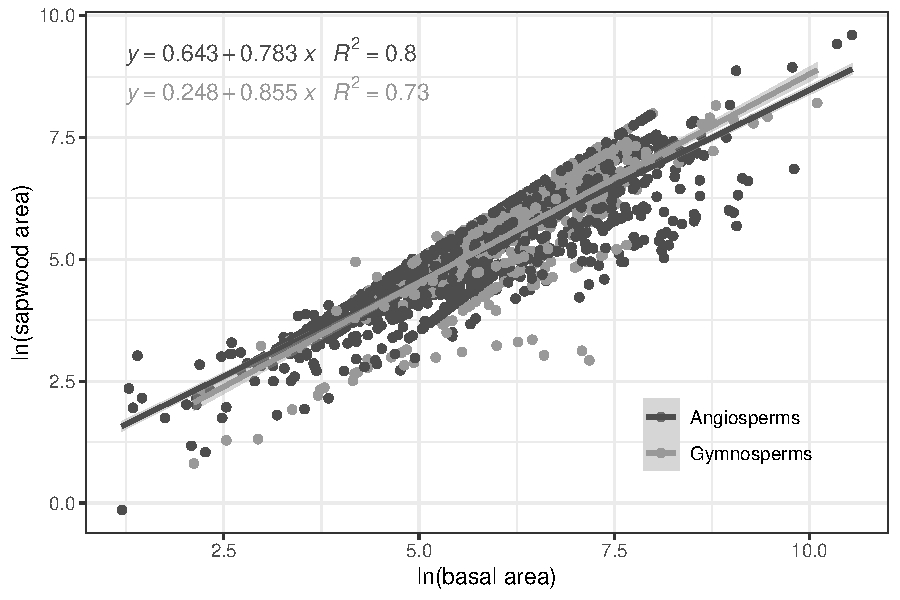
\includegraphics[width=1\linewidth]{figure/appendixC/dbh_sw} 

}

\caption[SAPFLUXNET global scaling relationship between basal area and sapwood area. Shaded areas are 95\% model confidence interval.]{SAPFLUXNET global scaling relationship between basal area and sapwood area. Shaded areas are 95\% model confidence interval.}\label{fig:unnamed-chunk-8}
\end{figure}
\setlength{\abovecaptionskip}{0pt}

\newpage

\setlength{\abovecaptionskip}{15pt}
\begin{figure}[H]

{\centering 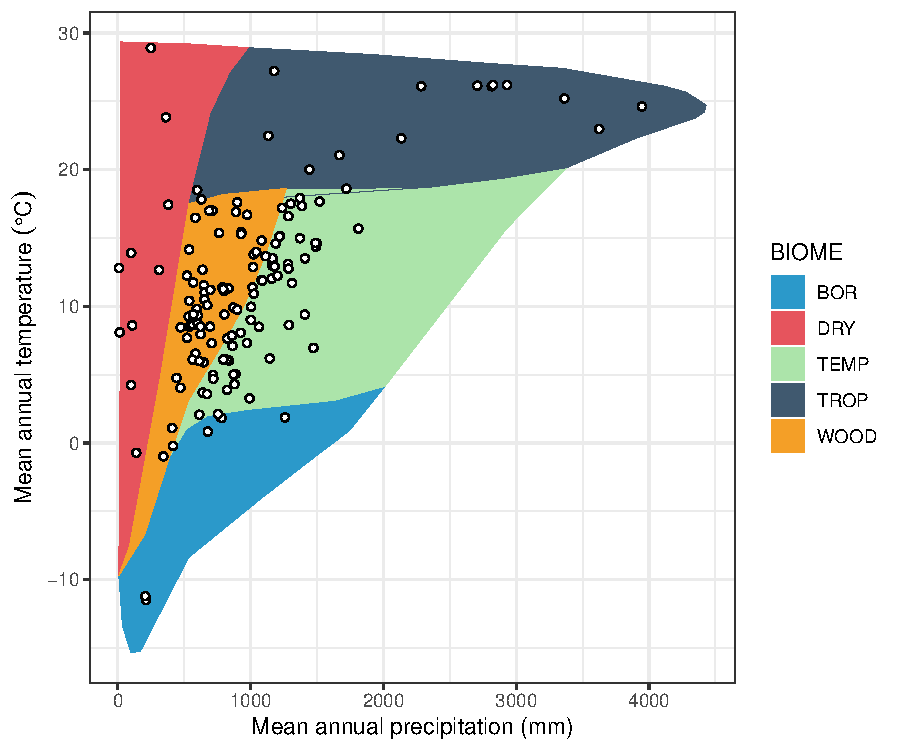
\includegraphics[width=1\linewidth]{figure/appendixC/gg_biomes} 

}

\caption[Bioclimatic distribution of the SAPFLUXNET datasets used in the study.]{Bioclimatic distribution of the SAPFLUXNET datasets used in the study. Points show the different datasets in a Whittaker diagram showing the classification of the aggregated biomes used in the study.}\label{fig:unnamed-chunk-9}
\end{figure}
\setlength{\abovecaptionskip}{0pt}

\newpage

\setlength{\abovecaptionskip}{15pt}
\begin{figure}[H]

{\centering \includegraphics[width=1\linewidth]{figure/appendixC/var_maps} 

}

\caption[Global projection of climatic, soil and stand structure variables.]{Global projection of climatic, soil and stand structure variables. log(PPET): logarithm of precipitation over potential evapotraspiration [log(mm \text{$mm^{-1}$})]; log(\text{$P-PET_{sd}$}): logarithm of the standard deviation of the difference between precipitation and potential evapotranspiration [log(mm)]; Clay: percentage of clay in the soil; Total N: total nitrogen in the soil [g \text{$kg^{-1}$}];  Bedrock [cm]; Stand height [m]; LAI: leaf area index [\text{$m^2$ $m^{-2}$}]. Total N values above 5 g \text{$kg^{-1}$} were truncated.}\label{fig:unnamed-chunk-10}
\end{figure}
\setlength{\abovecaptionskip}{0pt}

\newpage

\setlength{\abovecaptionskip}{15pt}
\begin{figure}[hbt!]

{\centering 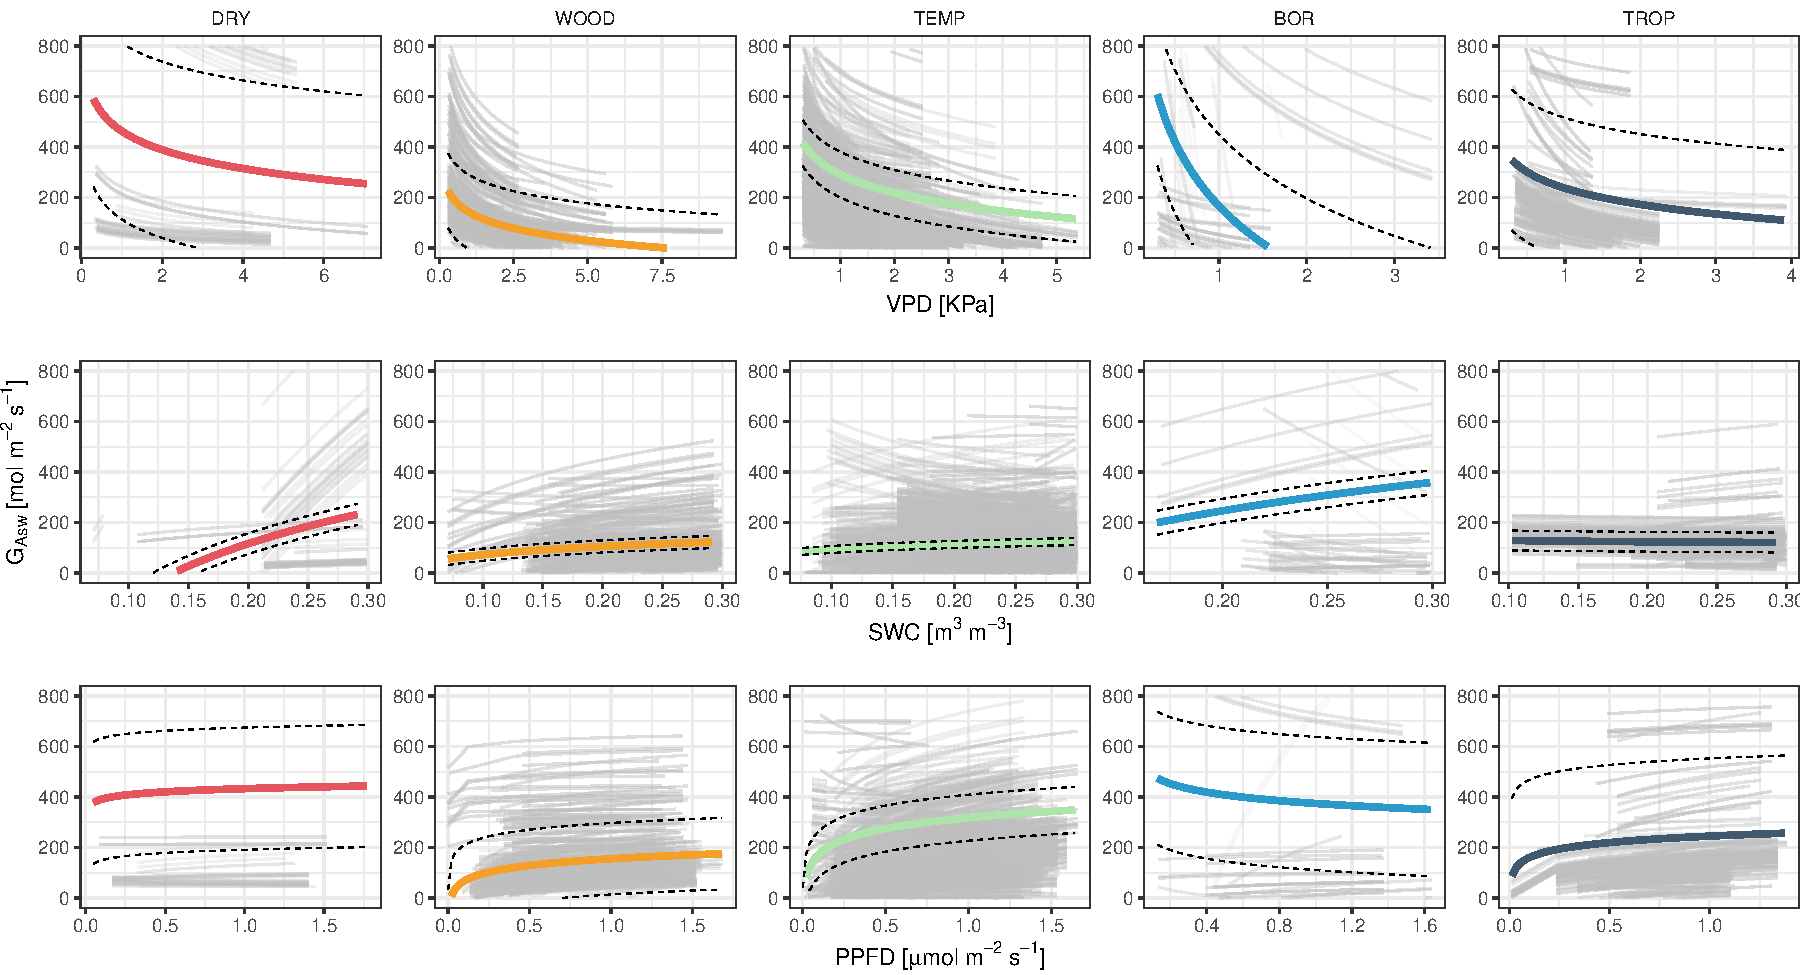
\includegraphics[width=1\linewidth]{figure/appendixC/spa_plots} 

}

\caption[Log relationships of the three environmental variables estimated with the TOTAL model (VPD + SWC + PPFD) and grouped by biome.]{Log relationships of the three environmental variables estimated with the TOTAL model (VPD + SWC + PPFD) and grouped by biome. Coloured lines are biome average models calculated from the Log-linear models predictions using LMM with Gs as response variable and the neperian logarithm of the environmental constrains as explanatory variables. Dashed line shows standard error of the average models calculated with bootstrap prediction using 100 simulations.}\label{fig:unnamed-chunk-11}
\end{figure}
\setlength{\abovecaptionskip}{0pt} \newpage

\section{Tables C}\label{tables-c}

\begingroup\fontsize{6}{8}\selectfont
\begin{longtable}[t]{ccccccc}
\caption[SAPFLUXNET sites included in the study. Biome was calculated using Whittaker diagram.]{\label{tab:unnamed-chunk-12}SAPFLUXNET sites included in the study. Biome was calculated using Whittaker diagram. *Indicates that the biome was manually adjusted and confirmed by SAPFLUXNET contributors.}\\
\toprule
Site code & Latitude & Longitude & Biome & \# Tree-days & \# Species & \# Trees\\
\midrule
\endfirsthead
\caption[]{\label{tab:unnamed-chunk-12}SAPFLUXNET sites included in the study. Biome was calculated using Whittaker diagram. *Indicates that the biome was manually adjusted and confirmed by SAPFLUXNET contributors. \textit{(continued)}}\\
\toprule
Site code & Latitude & Longitude & Biome & \# Tree-days & \# Species & \# Trees\\
\midrule
\endhead
\
\endfoot
\bottomrule
\endlastfoot
AUS\_CAN\_ST1\_EUC & -37.58 & 149.17 & WOOD & 337 & 1 & 12\\
AUS\_CAN\_ST2\_MIX & -37.58 & 149.17 & WOOD & 712 & 2 & 22\\
AUS\_CAN\_ST3\_ACA & -37.58 & 149.17 & WOOD & 409 & 1 & 12\\
AUS\_CAR\_THI\_CON & -38.38 & 146.68 & TEMP & 54 & 1 & 7\\
AUS\_ELL\_UNB & -36.78 & 146.58 & TEMP & 105 & 1 & 2\\
AUS\_MAR\_UBD & -37.69 & 145.56 & TEMP & 50 & 3 & 5\\
AUS\_MAR\_UBW & -37.89 & 145.57 & TEMP & 105 & 3 & 5\\
AUS\_WOM & -37.42 & 144.09 & TEMP & 2130 & 2 & 11\\
AUT\_PAT\_FOR & 47.21 & 11.45 & BOR & 149 & 1 & 3\\
AUT\_PAT\_KRU & 47.21 & 11.45 & BOR & 70 & 1 & 3\\
AUT\_PAT\_TRE & 47.21 & 11.45 & BOR & 81 & 1 & 3\\
BRA\_CAM & -22.69 & -45.52 & TROP & 79 & 1 & 5\\
BRA\_CAX\_CON & -1.79 & -51.43 & TROP & 525 & 8 & 15\\
CAN\_TUR\_P39\_PRE & 42.71 & -80.36 & TEMP & 1021 & 1 & 18\\
CAN\_TUR\_P74 & 42.71 & -80.35 & TEMP & 1997 & 1 & 16\\
CHN\_ARG\_GWS & 41.38 & 89.94 & DRY & 174 & 1 & 2\\
CHN\_HOR\_AFF & 42.72 & 122.37 & WOOD & 1366 & 1 & 16\\
CHN\_YIN\_ST1 & 42.45 & 85.72 & DRY & 105 & 1 & 5\\
CRI\_TAM\_TOW & 10.39 & -84.63 & TROP & 666 & 17 & 26\\
CZE\_BIL\_BIL & 49.25 & 16.69 & TEMP & 238 & 1 & 6\\
CZE\_KRT\_KRT & 49.32 & 16.75 & TEMP & 238 & 1 & 6\\
CZE\_LAN & 48.68 & 16.95 & TEMP & 1093 & 3 & 17\\
CZE\_RAJ\_RAJ & 49.44 & 16.70 & TEMP & 274 & 1 & 6\\
CZE\_SOB\_SOB & 49.25 & 16.69 & TEMP & 655 & 1 & 6\\
CZE\_STI & 49.04 & 17.97 & TEMP & 263 & 1 & 8\\
CZE\_UTE\_BPO & 49.28 & 16.65 & TEMP & 234 & 1 & 6\\
DEU\_HIN\_OAK & 53.33 & 13.19 & TEMP & 482 & 1 & 8\\
DEU\_HIN\_TER & 53.33 & 13.19 & TEMP & 1052 & 2 & 16\\
DEU\_MER\_BEE\_NON & 49.27 & 7.81 & TEMP & 495 & 1 & 8\\
DEU\_MER\_DOU\_NON & 49.27 & 7.81 & TEMP & 491 & 1 & 7\\
DEU\_MER\_MIX\_NON & 49.27 & 7.81 & TEMP & 1108 & 2 & 17\\
DEU\_STE\_2P3 & 53.10 & 13.00 & TEMP & 722 & 1 & 10\\
DEU\_STE\_4P5 & 53.10 & 13.00 & TEMP & 327 & 1 & 10\\
ESP\_ALT\_ARM & 40.78 & -2.33 & WOOD & 1990 & 3 & 15\\
ESP\_ALT\_HUE & 40.79 & -2.29 & WOOD & 967 & 2 & 8\\
ESP\_ALT\_TRI & 40.80 & -2.23 & WOOD & 1522 & 2 & 12\\
ESP\_CAN & 41.43 & 2.07 & WOOD & 2317 & 4 & 21\\
ESP\_GUA\_VAL & 40.90 & -4.03 & WOOD & 2100 & 1 & 24\\
ESP\_LAS & 28.31 & -16.57 & WOOD & 1778 & 1 & 10\\
ESP\_MAJ\_MAI & 39.94 & -5.77 & WOOD & 978 & 1 & 6\\
ESP\_MON\_SIE\_NAT & 41.12 & -3.50 & WOOD & 1250 & 3 & 20\\
ESP\_RIN & 40.60 & -6.02 & WOOD & 502 & 1 & 8\\
ESP\_RON\_PIL & 36.69 & -5.02 & TEMP & 911 & 2 & 12\\
ESP\_TIL\_MIX & 41.33 & 1.01 & WOOD & 3434 & 2 & 32\\
ESP\_TIL\_OAK & 41.33 & 1.01 & WOOD & 717 & 1 & 10\\
ESP\_TIL\_PIN & 41.33 & 1.01 & WOOD & 589 & 1 & 9\\
ESP\_VAL\_BAR & 42.20 & 1.82 & WOOD & 837 & 1 & 12\\
ESP\_VAL\_SOR & 42.20 & 1.81 & WOOD & 1109 & 1 & 13\\
ESP\_YUN\_C1 & 36.72 & -4.97 & WOOD & 619 & 1 & 6\\
ESP\_YUN\_C2 & 36.72 & -4.97 & WOOD & 288 & 1 & 6\\
FIN\_HYY\_SME & 61.85 & 24.29 & TEMP & 34 & 2 & 4\\
FIN\_PET & 69.49 & 27.23 & BOR & 118 & 1 & 7\\
FRA\_FON & 48.48 & 2.78 & TEMP & 276 & 1 & 3\\
FRA\_HES\_HE1\_NON & 48.67 & 7.06 & TEMP & 620 & 1 & 10\\
FRA\_HES\_HE2\_NON & 48.67 & 7.06 & TEMP & 1347 & 1 & 10\\
FRA\_PUE & 43.74 & 3.60 & WOOD & 5229 & 1 & 25\\
GBR\_ABE\_PLO & 56.62 & -3.80 & TEMP & 486 & 1 & 15\\
GBR\_DEV\_CON & 56.03 & -3.72 & TEMP & 133 & 1 & 4\\
GBR\_GUI\_ST1 & 57.27 & -4.82 & TEMP & 398 & 1 & 15\\
GBR\_GUI\_ST2 & 57.27 & -4.82 & TEMP & 298 & 1 & 9\\
GBR\_GUI\_ST3 & 57.27 & -4.82 & TEMP & 249 & 1 & 8\\
GUF\_GUY\_GUY & 5.28 & -52.92 & TROP & 246 & 6 & 6\\
GUF\_GUY\_ST2 & 5.28 & -52.91 & TROP & 369 & 7 & 11\\
GUF\_NOU\_PET & 4.08 & -52.68 & TROP & 562 & 10 & 22\\
HUN\_SIK & 47.93 & 20.44 & WOOD & 365 & 2 & 4\\
ISR\_YAT\_YAT & 31.34 & 35.05 & DRY & 3704 & 1 & 24\\
ITA\_FEI\_S17 & 46.69 & 10.61 & TEMP & 244 & 1 & 6\\
ITA\_KAE\_S20 & 46.70 & 10.61 & BOR & 325 & 1 & 6\\
ITA\_MUN & 46.68 & 10.58 & TEMP & 384 & 1 & 6\\
ITA\_REN & 46.59 & 11.43 & TEMP & 247 & 3 & 8\\
ITA\_RUN\_N20 & 46.70 & 10.64 & BOR & 331 & 2 & 8\\
MEX\_COR\_YP & 19.49 & -97.04 & TEMP & 119 & 1 & 8\\
NLD\_LOO & 52.17 & 5.74 & TEMP & 621 & 1 & 6\\
NLD\_SPE\_DOU & 52.25 & 5.69 & TEMP & 107 & 1 & 3\\
NZL\_HUA\_HUA & -36.80 & 174.49 & TEMP & 243 & 1 & 6\\
PRT\_LEZ\_ARN & 38.83 & -8.82 & WOOD & 403 & 1 & 4\\
PRT\_MIT & 38.54 & -8.00 & WOOD & 494 & 1 & 4\\
PRT\_PIN & 38.25 & -8.76 & WOOD & 1233 & 2 & 20\\
RUS\_CHE\_Y4 & 68.74 & 161.41 & BOR & 447 & 1 & 11\\
RUS\_FYO & 56.46 & 32.92 & TEMP & 1132 & 3 & 17\\
RUS\_POG\_VAR & 56.36 & 92.95 & TEMP & 603 & 3 & 9\\
SEN\_SOU\_PRE & 16.34 & -15.43 & DRY & 466 & 1 & 3\\
SWE\_NOR\_ST1\_BEF & 60.09 & 17.48 & TEMP & 653 & 2 & 22\\
SWE\_NOR\_ST2 & 60.09 & 17.48 & TEMP & 175 & 2 & 12\\
SWE\_NOR\_ST3 & 60.09 & 17.48 & TEMP & 810 & 2 & 37\\
SWE\_NOR\_ST5\_REF & 60.08 & 17.48 & TEMP & 712 & 3 & 35\\
SWE\_SKO\_MIN & 58.36 & 12.15 & TEMP & 533 & 1 & 11\\
SWE\_SKY\_38Y & 60.13 & 17.84 & TEMP & 326 & 1 & 12\\
SWE\_SKY\_68Y & 60.10 & 17.83 & TEMP & 664 & 2 & 12\\
SWE\_SVA\_MIX\_NON & 64.26 & 19.77 & TEMP & 861 & 2 & 20\\
THA\_KHU & 15.27 & 103.08 & TROP & 411 & 1 & 6\\
USA\_BNZ\_BLA & 64.70 & -148.32 & BOR & 797 & 1 & 6\\
USA\_CHE\_ASP & 45.94 & -90.27 & TEMP & 3548 & 6 & 149\\
USA\_CHE\_MAP & 45.95 & -90.26 & TEMP & 2651 & 2 & 153\\
USA\_DUK\_HAR & 36.98 & -79.09 & TEMP & 495 & 6 & 34\\
USA\_HIL\_HF2 & 36.22 & -78.86 & TEMP & 228 & 5 & 23\\
USA\_INM & 39.32 & -86.41 & TEMP & 766 & 6 & 9\\
USA\_MOR\_SF & 39.32 & -86.41 & TEMP & 285 & 4 & 6\\
USA\_NWH & 34.58 & -91.26 & TEMP & 248 & 2 & 10\\
USA\_ORN\_ST1\_AMB & 35.90 & -84.33 & TEMP & 247 & 1 & 8\\
USA\_PAR\_FER & 35.80 & -76.67 & TEMP & 467 & 1 & 8\\
USA\_PER\_PER & 30.21 & -83.87 & TROP & 6269 & 1 & 80\\
USA\_PJS\_P04\_AMB & 34.39 & -106.53 & DRY & 2313 & 2 & 10\\
USA\_PJS\_P08\_AMB & 34.39 & -106.53 & DRY & 2262 & 2 & 10\\
USA\_PJS\_P12\_AMB & 34.39 & -106.53 & DRY & 2350 & 2 & 10\\
USA\_SIL\_OAK\_1PR & 39.92 & -74.60 & TEMP & 1210 & 4 & 18\\
USA\_SIL\_OAK\_2PR & 39.92 & -74.60 & TEMP & 2275 & 4 & 22\\
USA\_SMI\_SER & 38.89 & -76.56 & TEMP & 1045 & 5 & 31\\
USA\_SWH & 34.11 & -91.13 & TEMP & 511 & 2 & 16\\
USA\_SYL\_HL1 & 46.24 & -89.35 & TEMP & 3130 & 3 & 48\\
USA\_SYL\_HL2 & 46.24 & -89.35 & TEMP & 1631 & 4 & 20\\
USA\_TNB & 36.47 & -84.70 & TEMP & 583 & 4 & 8\\
USA\_TNO & 35.97 & -84.28 & TEMP & 680 & 5 & 9\\
USA\_TNP & 35.96 & -84.29 & TEMP & 806 & 5 & 9\\
USA\_UMB\_CON & 45.56 & -84.71 & TEMP & 5840 & 5 & 57\\
USA\_UMB\_GIR & 45.56 & -84.70 & TEMP & 5867 & 4 & 57\\
USA\_WIL\_WC1 & 45.81 & -90.09 & TEMP & 639 & 5 & 16\\
USA\_WVF & 39.06 & -79.69 & TEMP & 488 & 5 & 8\\
ZAF\_FRA\_FRA & -33.88 & 19.06 & WOOD & 220 & 1 & 3\\
ZAF\_RAD & -34.08 & 19.11 & WOOD & 303 & 1 & 3\\
ZAF\_SOU\_SOU & -34.09 & 19.09 & WOOD & 198 & 1 & 2\\
ZAF\_WEL\_SOR & -33.48 & 18.96 & WOOD & 356 & 1 & 3\\*
\end{longtable}
\endgroup{} \newpage
\begin{table}[H]

\caption[SAPFLUXNET stand treatments included in the this study (Poyatos $et$ $al.$ 2020).]{\label{tab:unnamed-chunk-13}SAPFLUXNET stand treatments included in the this study (Poyatos $et$ $al.$ 2020).}
\centering
\resizebox{\linewidth}{!}{
\begin{tabular}[t]{l}
\toprule
Plot treatment\\
\midrule
\\
None\\
Control\\
control\\
Ambient Control\\
Control - Unthinned\\
natural conditions\\
Reference\\
1Premortality\\
2premortality\\
distructive sampling\\
Girdling early successional\\
Pre-thinning\\
Before thinning\\
Before Thinning\\
non thinned\\
none (periodict thinning every 5-6 years  20 to 25\% of basal area)\\
Radiation Level\\
AMBIENT CO2 FACE rings\\
fertilization at plantation\\
AcaciaMonoculture\\
MixtureEucalyptusAndAcacia\\
EucalyptusMonoculture\\
Pre Irrigation\\
\bottomrule
\end{tabular}}
\end{table}\newpage
\begin{landscape}
\begingroup\fontsize{5}{7}\selectfont
\begin{longtable}[t]{>{\centering\arraybackslash}p{8em}>{\centering\arraybackslash}p{3.5em}>{\centering\arraybackslash}p{3.5em}>{\centering\arraybackslash}p{3.5em}>{\centering\arraybackslash}p{3.5em}>{\centering\arraybackslash}p{3.5em}>{\centering\arraybackslash}p{3.5em}>{\centering\arraybackslash}p{3.5em}>{\centering\arraybackslash}p{3.5em}>{\centering\arraybackslash}p{3.5em}>{\centering\arraybackslash}p{3.5em}>{\centering\arraybackslash}p{3.5em}>{\centering\arraybackslash}p{3.5em}>{\centering\arraybackslash}p{3.5em}c}
\caption[Summary table of plot level.]{\label{tab:unnamed-chunk-14}Summary table of site level $\text{R}^2_{\text{VPD}}$, $\text{R}^2_{\text{SWC}}$, $\text{R}^2_{\text{PPFD}}$, climate, soil properties and vegetation structure data. PPET is in [mm $\text{mm}^{-1}$], $\text{P-PET}_{\text{sd}}$ is in [mm], Clay and Sand are in [\%], Total N is in [g $\text{kg}^{-1}$], Stand height is in [m], LAI is in [$\text{m}^2_{\text{leaves}}\;\text{m}^2_{\text{soil}}$]. Letters show data source: a = SAPFLUXNET, b = Global rasters, c = SAPFLUXNET plant height.}\\
\toprule
\rotatebox{45}{Site code} & \rotatebox{45}{\text{$R^2_{vpd}$}} & \rotatebox{45}{\text{$R^2_{swc}$}} & \rotatebox{45}{\text{$R^2_{ppfd}$}} & \rotatebox{45}{Relimp VPD} & \rotatebox{45}{Relimp SWC} & \rotatebox{45}{Relimp PPFD} & \rotatebox{45}{PPET} & \rotatebox{45}{\text{$P-PET_{sd}$}} & \rotatebox{45}{Clay} & \rotatebox{45}{Sand} & \rotatebox{45}{Total N} & \rotatebox{45}{Bedrock} & \rotatebox{45}{Stand height} & \rotatebox{45}{LAI}\\
\midrule
\endfirsthead
\caption[]{\label{tab:unnamed-chunk-14}Summary table of site level $\text{R}^2_{\text{VPD}}$, $\text{R}^2_{\text{SWC}}$, $\text{R}^2_{\text{PPFD}}$, climate, soil properties and vegetation structure data. PPET is in [mm $\text{mm}^{-1}$], $\text{P-PET}_{\text{sd}}$ is in [mm], Clay and Sand are in [\%], Total N is in [g $\text{kg}^{-1}$], Stand height is in [m], LAI is in [$\text{m}^2_{\text{leaves}}\;\text{m}^2_{\text{soil}}$]. Letters show data source: a = SAPFLUXNET, b = Global rasters, c = SAPFLUXNET plant height. \textit{(continued)}}\\
\toprule
\rotatebox{45}{Site code} & \rotatebox{45}{\text{$R^2_{vpd}$}} & \rotatebox{45}{\text{$R^2_{swc}$}} & \rotatebox{45}{\text{$R^2_{ppfd}$}} & \rotatebox{45}{Relimp VPD} & \rotatebox{45}{Relimp SWC} & \rotatebox{45}{Relimp PPFD} & \rotatebox{45}{PPET} & \rotatebox{45}{\text{$P-PET_{sd}$}} & \rotatebox{45}{Clay} & \rotatebox{45}{Sand} & \rotatebox{45}{Total N} & \rotatebox{45}{Bedrock} & \rotatebox{45}{Stand height} & \rotatebox{45}{LAI}\\
\midrule
\endhead
\
\endfoot
\bottomrule
\endlastfoot
AUS\_CAN\_ST1\_EUC & 0.74 & 0.44 & 0.54 & 0.65 & 0.35 & 0.00 & 1.23 & 47.52 & 26.30 b & 45.10 b & 1.02 & 184 & 22.00 a & 1.39 a\\
AUS\_CAN\_ST2\_MIX & 0.91 & 0.65 & 0.76 & 0.87 & 0.13 & 0.00 & 1.23 & 47.52 & 26.30 b & 45.10 b & 1.02 & 184 & 21.80 a & 2.07 a\\
AUS\_CAN\_ST3\_ACA & 0.85 & 0.67 & 0.74 & 0.87 & 0.12 & 0.01 & 1.23 & 47.52 & 26.30 b & 45.10 b & 1.02 & 184 & 11.80 a & 1.35 a\\
AUS\_CAR\_THI\_CON & 0.67 & 0.00 & 0.00 & 0.99 & 0.00 & 0.01 & 1.36 & 49.01 & 27.20 b & 44.30 b & 2.34 & 111 & 17.21 a & 4.80 a\\
AUS\_ELL\_UNB & 0.87 & 0.44 & 0.76 & 0.97 & 0.00 & 0.03 & 1.08 & 67.16 & 26.70 b & 48.50 b & 1.95 & 63 & 25.00 a & 6.20 b\\
AUS\_MAR\_UBD & 0.79 & 0.53 & 0.69 & 0.71 & 0.29 & 0.00 & 1.35 & 70.37 & 26.60 b & 44.60 b & 1.90 & 89 & 25.00 a & 2.10 a\\
AUS\_MAR\_UBW & 0.90 & 0.81 & 0.82 & 0.90 & 0.00 & 0.09 & 1.21 & 65.38 & 27.90 b & 43.90 b & 2.00 & 173 & 40.00 a & 2.30 a\\
AUS\_WOM & 0.82 & 0.52 & 0.49 & 0.79 & 0.00 & 0.20 & 1.09 & 69.35 & 25.90 b & 52.90 b & 1.97 & 172 & 22.00 a & 2.20 a\\
AUT\_PAT\_FOR & 0.78 & 0.73 & 0.68 & 0.82 & 0.09 & 0.09 & 2.17 & 16.78 & 5.00 a & 60.00 a & 3.94 & 180 & 12.00 a & 4.30 b\\
AUT\_PAT\_KRU & 0.61 & 0.45 & 0.50 & 0.77 & 0.06 & 0.17 & 2.17 & 16.78 & 5.00 a & 60.00 a & 3.94 & 180 & 0.75 a & 4.30 b\\
AUT\_PAT\_TRE & 0.58 & 0.27 & 0.19 & 0.70 & 0.30 & 0.00 & 2.17 & 16.78 & 5.00 a & 60.00 a & 3.94 & 180 & 4.00 a & 4.30 b\\
BRA\_CAM & 0.83 & 0.68 & 0.69 & 0.65 & 0.28 & 0.07 & 1.66 & 88.82 & 27.60 b & 52.00 b & 2.26 & 200 & 12.00 a & 5.30 a\\
BRA\_CAX\_CON & 0.79 & 0.74 & 0.73 & 0.70 & 0.00 & 0.30 & 1.90 & 122.90 & 8.00 a & 79.00 a & 1.45 & 197 & 38.00 b & 5.30 a\\
CAN\_TUR\_P39\_PRE & 0.59 & 0.37 & 0.34 & 0.71 & 0.08 & 0.21 & 1.39 & 42.08 & 1.00 a & 98.00 a & 1.58 & 200 & 23.40 a & 5.30 a\\
CAN\_TUR\_P74 & 0.26 & 0.47 & 0.14 & 0.32 & 0.38 & 0.30 & 1.39 & 41.87 & 1.00 a & 98.00 a & 1.60 & 200 & 16.20 a & 6.70 a\\
CHN\_ARG\_GWS & 0.42 & 0.32 & 0.27 & 0.51 & 0.47 & 0.01 & 0.01 & 63.51 & 17.70 b & 46.00 b & 0.70 & 172 & 7.90 a & 0.36 a\\
CHN\_HOR\_AFF & 0.39 & 0.38 & 0.34 & 0.25 & 0.75 & 0.00 & 0.59 & 31.24 & 8.00 a & 83.00 a & 1.00 & 200 & 9.05 a & 1.61 a\\
CHN\_YIN\_ST1 & 0.47 & 0.45 & 0.44 & 0.63 & 0.18 & 0.20 & 0.19 & 35.09 & 20.80 b & 32.90 b & 2.41 & 148 & 10.60 a & 0.50 b\\
CRI\_TAM\_TOW & 0.73 & 0.73 & 0.73 & 0.46 & 0.11 & 0.44 & 3.57 & 159.99 & 36.10 b & 34.70 b & 2.75 & 200 & 30.60 a & 3.30 a\\
CZE\_BIL\_BIL & 0.54 & 0.50 & 0.41 & 0.57 & 0.20 & 0.23 & 0.71 & 28.98 & 29.60 b & 27.40 b & 1.91 & 200 & 14.00 a & 6.00 b\\
CZE\_KRT\_KRT & 0.57 & 0.45 & 0.30 & 0.58 & 0.03 & 0.39 & 0.85 & 27.00 & 26.00 b & 27.40 b & 2.10 & 200 & 17.00 a & 5.70 b\\
CZE\_LAN & 0.79 & 0.76 & 0.72 & 0.67 & 0.08 & 0.25 & 0.66 & 37.49 & 17.80 a & 71.80 a & 2.46 & 200 & 36.00 a & 6.04 a\\
CZE\_RAJ\_RAJ & 0.38 & 0.40 & 0.43 & 0.33 & 0.07 & 0.60 & 0.99 & 26.14 & 21.80 b & 33.90 b & 1.96 & 200 & 18.00 a & 4.60 b\\
CZE\_SOB\_SOB & 0.48 & 0.45 & 0.14 & 0.52 & 0.25 & 0.23 & 0.71 & 28.98 & 29.60 b & 27.40 b & 1.91 & 200 & 21.00 a & 6.00 b\\
CZE\_STI & 0.54 & 0.32 & 0.39 & 0.70 & 0.18 & 0.12 & 1.13 & 27.10 & 34.20 a & 47.60 a & 1.65 & 200 & 31.00 a & 5.50 a\\
CZE\_UTE\_BPO & 0.62 & 0.65 & 0.52 & 0.46 & 0.16 & 0.38 & 0.75 & 29.86 & 26.70 b & 23.80 b & 2.71 & 200 & 18.00 a & 6.10 b\\
DEU\_HIN\_OAK & 0.43 & 0.19 & 0.33 & 0.92 & 0.07 & 0.01 & 0.95 & 35.10 & 17.90 b & 49.90 b & 2.42 & 200 & 31.45 c & 5.70 b\\
DEU\_HIN\_TER & 0.31 & 0.22 & 0.24 & 0.76 & 0.01 & 0.24 & 0.95 & 35.10 & 18.00 b & 50.50 b & 2.05 & 200 & 24.43 c & 5.60 b\\
DEU\_MER\_BEE\_NON & 0.47 & 0.27 & 0.29 & 0.76 & 0.06 & 0.18 & 1.48 & 47.33 & 4.00 a & 71.00 a & 2.56 & 200 & 23.00 a & 5.90 a\\
DEU\_MER\_DOU\_NON & 0.45 & 0.25 & 0.22 & 0.60 & 0.31 & 0.10 & 1.48 & 47.33 & 4.00 a & 71.00 a & 2.56 & 200 & 29.00 a & 5.30 a\\
DEU\_MER\_MIX\_NON & 0.41 & 0.23 & 0.26 & 0.82 & 0.02 & 0.16 & 1.48 & 47.33 & 4.00 a & 71.00 a & 2.56 & 200 & 30.00 a & 6.10 a\\
DEU\_STE\_2P3 & 0.56 & 0.15 & 0.30 & 0.86 & 0.09 & 0.05 & 0.90 & 37.45 & 2.50 a & 92.50 a & 3.28 & 200 & 27.20 a & 4.30 b\\
DEU\_STE\_4P5 & 0.48 & 0.27 & 0.31 & 0.64 & 0.28 & 0.09 & 0.90 & 37.45 & 2.50 a & 92.50 a & 3.28 & 200 & 27.20 a & 4.30 b\\
ESP\_ALT\_ARM & 0.51 & 0.30 & 0.29 & 0.91 & 0.01 & 0.09 & 0.66 & 65.80 & 21.90 b & 41.50 b & 1.27 & 187 & 19.00 b & 1.09 a\\
ESP\_ALT\_HUE & 0.47 & 0.22 & 0.18 & 0.78 & 0.02 & 0.21 & 0.51 & 63.08 & 21.60 b & 35.90 b & 1.46 & 200 & 8.64 c & 1.50 b\\
ESP\_ALT\_TRI & 0.58 & 0.44 & 0.31 & 0.80 & 0.07 & 0.12 & 0.57 & 63.48 & 21.00 b & 40.00 b & 1.31 & 196 & 4.89 a & 1.60 b\\
ESP\_CAN & 0.55 & 0.40 & 0.34 & 0.74 & 0.02 & 0.24 & 0.94 & 46.91 & 32.90 b & 28.30 b & 1.76 & 179 & 10.80 a & 3.30 a\\
ESP\_GUA\_VAL & 0.51 & 0.28 & 0.23 & 0.69 & 0.00 & 0.31 & 0.68 & 69.09 & 24.80 b & 40.90 b & 1.27 & 200 & 12.00 a & 3.80 a\\
ESP\_LAS & 0.37 & 0.25 & 0.07 & 0.57 & 0.37 & 0.06 & 1.63 & 37.89 & 1.00 a & 70.00 a & 1.65 & 197 & 10.30 a & 3.60 a\\
ESP\_MAJ\_MAI & 0.56 & 0.43 & 0.28 & 0.73 & 0.14 & 0.12 & 0.76 & 97.45 & 9.00 a & 80.00 a & 1.18 & 200 & 7.00 a & 0.30 a\\
ESP\_MON\_SIE\_NAT & 0.25 & 0.20 & 0.22 & 0.49 & 0.09 & 0.42 & 0.62 & 63.05 & 20.80 b & 41.90 b & 1.45 & 200 & 22.00 a & 3.30 b\\
ESP\_RIN & 0.83 & 0.61 & 0.59 & 0.97 & 0.00 & 0.03 & 0.85 & 76.30 & 15.00 a & 9.00 a & 2.17 & 200 & 7.40 a & 3.40 a\\
ESP\_RON\_PIL & 0.37 & 0.25 & 0.17 & 0.60 & 0.07 & 0.33 & 1.05 & 93.66 & 18.00 a & 30.00 a & 1.86 & 200 & 2.60 a & 0.90 b\\
ESP\_TIL\_MIX & 0.45 & 0.36 & 0.22 & 0.55 & 0.09 & 0.36 & 0.77 & 48.10 & 20.00 a & 60.00 a & 1.44 & 162 & 14.20 a & 3.27 a\\
ESP\_TIL\_OAK & 0.31 & 0.38 & 0.18 & 0.45 & 0.15 & 0.40 & 0.77 & 48.10 & 20.00 a & 60.00 a & 1.44 & 162 & 5.00 a & 4.59 a\\
ESP\_TIL\_PIN & 0.37 & 0.45 & 0.08 & 0.43 & 0.37 & 0.20 & 0.79 & 48.10 & 20.00 a & 60.00 a & 1.78 & 188 & 18.30 a & 1.02 a\\
ESP\_VAL\_BAR & 0.61 & 0.22 & 0.29 & 0.90 & 0.00 & 0.10 & 0.70 & 34.07 & 32.63 a & 9.81 a & 1.94 & 200 & 10.60 a & 2.10 a\\
ESP\_VAL\_SOR & 0.58 & 0.36 & 0.26 & 0.73 & 0.14 & 0.13 & 0.78 & 32.15 & 20.00 a & 60.00 a & 2.04 & 200 & 11.00 a & 2.40 a\\
ESP\_YUN\_C1 & 0.37 & 0.50 & 0.24 & 0.28 & 0.56 & 0.16 & 0.83 & 93.65 & 29.00 a & 22.00 a & 1.37 & 197 & 10.60 a & 2.20 b\\
ESP\_YUN\_C2 & 0.28 & 0.62 & 0.27 & 0.21 & 0.43 & 0.37 & 0.78 & 91.33 & 29.00 a & 22.00 a & 1.37 & 188 & 11.60 a & 2.50 b\\
FIN\_HYY\_SME & 0.57 & 0.49 & 0.62 & 0.12 & 0.86 & 0.02 & 1.20 & 38.32 & 6.50 a & 37.00 a & 1.67 & 200 & 18.00 a & 1.30 a\\
FIN\_PET & 0.59 & 0.50 & 0.58 & 0.47 & 0.37 & 0.16 & 1.13 & 26.34 & 7.30 b & 60.80 b & 5.08 & 200 & 3.76 a & 0.61 a\\
FRA\_FON & 0.78 & 0.68 & 0.68 & 0.70 & 0.17 & 0.13 & 0.89 & 45.10 & 19.00 a & 37.00 a & 1.26 & 200 & 28.00 a & 6.00 a\\
FRA\_HES\_HE1\_NON & 0.46 & 0.57 & 0.41 & 0.45 & 0.25 & 0.30 & 1.31 & 47.72 & 25.00 a & 8.00 a & 1.41 & 200 & 12.80 a & 6.00 a\\
FRA\_HES\_HE2\_NON & 0.33 & 0.50 & 0.16 & 0.42 & 0.27 & 0.31 & 1.31 & 47.72 & 25.00 a & 8.00 a & 1.41 & 200 & 13.00 a & 6.00 a\\
FRA\_PUE & 0.49 & 0.52 & 0.33 & 0.51 & 0.18 & 0.30 & 1.27 & 70.16 & 39.00 a & 26.00 a & 1.69 & 195 & 5.00 a & 2.40 a\\
GBR\_ABE\_PLO & 0.40 & 0.37 & 0.35 & 0.51 & 0.22 & 0.27 & 1.92 & 47.48 & 10.00 a & 60.00 a & 3.70 & 179 & 10.00 a & 6.00 a\\
GBR\_DEV\_CON & 0.89 & 0.45 & 0.58 & 0.95 & 0.01 & 0.04 & 1.43 & 44.38 & 14.80 b & 56.90 b & 3.44 & 200 & 15.00 a & 1.92 a\\
GBR\_GUI\_ST1 & 0.84 & 0.79 & 0.78 & 0.68 & 0.00 & 0.32 & 3.19 & 68.11 & 3.70 b & 80.40 b & 14.26 & 197 & 11.00 a & 0.92 a\\
GBR\_GUI\_ST2 & 0.64 & 0.55 & 0.49 & 0.59 & 0.03 & 0.38 & 3.19 & 68.11 & 3.70 b & 80.40 b & 14.26 & 197 & 13.30 a & 0.94 a\\
GBR\_GUI\_ST3 & 0.86 & 0.82 & 0.79 & 0.73 & 0.03 & 0.24 & 3.19 & 68.11 & 3.70 b & 80.40 b & 14.26 & 197 & 14.30 a & 1.57 a\\
GUF\_GUY\_GUY & 0.97 & 0.89 & 0.94 & 0.82 & 0.05 & 0.12 & 2.88 & 135.18 & 43.00 a & 48.00 a & 1.53 & 200 & 35.00 a & 7.00 a\\
GUF\_GUY\_ST2 & 0.80 & 0.77 & 0.76 & 0.61 & 0.30 & 0.09 & 3.02 & 141.34 & 43.20 a & 47.80 a & 1.66 & 200 & 35.00 a & 6.70 a\\
GUF\_NOU\_PET & 0.76 & 0.53 & 0.66 & 1.00 & 0.00 & 0.00 & 2.69 & 158.16 & 59.20 a & 33.20 a & 2.22 & 200 & 35.00 a & 5.50 a\\
HUN\_SIK & 0.86 & 0.42 & 0.56 & 0.90 & 0.00 & 0.09 & 0.70 & 39.64 & 30.40 b & 44.00 b & 1.64 & 200 & 20.00 a & 7.00 a\\
ISR\_YAT\_YAT & 0.40 & 0.32 & 0.18 & 0.62 & 0.37 & 0.01 & 0.28 & 83.43 & 28.00 a & 31.00 a & 0.71 & 178 & 11.00 a & 1.70 a\\
ITA\_FEI\_S17 & 0.53 & 0.37 & 0.30 & 0.66 & 0.14 & 0.19 & 1.08 & 22.97 & 8.00 a & 76.00 a & 3.11 & 117 & 20.00 a & 3.10 b\\
ITA\_KAE\_S20 & 0.68 & 0.45 & 0.46 & 0.75 & 0.07 & 0.18 & 1.24 & 22.97 & 17.00 a & 50.00 a & 3.64 & 121 & 14.00 a & 2.60 b\\
ITA\_MUN & 0.63 & 0.48 & 0.42 & 0.62 & 0.31 & 0.06 & 0.80 & 29.87 & 7.00 a & 55.00 a & 1.93 & 188 & 18.00 a & 2.20 b\\
ITA\_REN & 0.85 & 0.77 & 0.79 & 0.95 & 0.02 & 0.04 & 1.61 & 12.59 & 17.70 b & 47.90 b & 2.73 & 143 & 27.00 b & 4.60 b\\
ITA\_RUN\_N20 & 0.84 & 0.73 & 0.74 & 0.94 & 0.02 & 0.04 & 1.39 & 15.28 & 14.00 a & 54.00 a & 3.33 & 123 & 18.70 a & 5.70 b\\
MEX\_COR\_YP & 0.68 & 0.24 & 0.31 & 0.78 & 0.05 & 0.18 & 1.42 & 81.77 & 22.20 b & 46.40 b & 2.94 & 200 & 7.00 a & 5.20 a\\
NLD\_LOO & 0.55 & 0.31 & 0.27 & 0.74 & 0.02 & 0.24 & 1.33 & 41.67 & 1.00 a & 99.00 a & 2.61 & 200 & 18.00 a & 2.20 a\\
NLD\_SPE\_DOU & 0.76 & 0.60 & 0.63 & 0.81 & 0.09 & 0.11 & 1.42 & 39.80 & 4.80 b & 80.70 b & 1.62 & 200 & 30.00 a & 4.50 a\\
NZL\_HUA\_HUA & 0.71 & 0.62 & 0.61 & 0.75 & 0.17 & 0.08 & 2.62 & 42.52 & 71.20 a & 13.20 a & 1.73 & 200 & 27.00 a & 6.60 b\\
PRT\_LEZ\_ARN & 0.70 & 0.23 & 0.25 & 0.77 & 0.02 & 0.21 & 0.72 & 77.42 & 5.04 a & 90.38 a & 1.52 & 200 & 12.00 a & 1.50 a\\
PRT\_MIT & 0.76 & 0.47 & 0.36 & 0.78 & 0.18 & 0.04 & 0.51 & 80.80 & 16.10 b & 64.50 b & 1.33 & 200 & 7.50 a & 0.55 a\\
PRT\_PIN & 0.65 & 0.50 & 0.36 & 0.66 & 0.33 & 0.01 & 0.76 & 74.76 & 16.60 b & 61.20 b & 1.26 & 200 & 12.60 a & 1.10 b\\
RUS\_CHE\_Y4 & 0.31 & 0.21 & 0.23 & 0.95 & 0.01 & 0.04 & 0.62 & 34.23 & 21.10 b & 23.20 b & 4.96 & 200 & 7.00 a & 1.30 b\\
RUS\_FYO & 0.72 & 0.62 & 0.62 & 0.88 & 0.00 & 0.12 & 1.24 & 30.87 & 18.20 b & 48.80 b & 3.77 & 198 & 23.50 a & 3.50 a\\
RUS\_POG\_VAR & 0.78 & 0.49 & 0.61 & 0.89 & 0.00 & 0.11 & 0.70 & 33.02 & 28.60 b & 37.50 b & 2.64 & 200 & 22.00 a & 2.80 b\\
SEN\_SOU\_PRE & 0.75 & 0.35 & 0.16 & 0.79 & 0.21 & 0.00 & 0.13 & 43.94 & 6.00 a & 90.00 a & 0.23 & 200 & 7.00 a & 0.22 a\\
SWE\_NOR\_ST1\_BEF & 0.75 & 0.62 & 0.62 & 0.68 & 0.19 & 0.13 & 1.07 & 36.70 & 5.80 a & 58.60 a & 2.63 & 185 & 28.70 a & 4.18 a\\
SWE\_NOR\_ST2 & 0.26 & 0.21 & 0.17 & 0.56 & 0.00 & 0.44 & 1.07 & 36.70 & 5.80 a & 58.60 a & 2.63 & 185 & 27.70 a & 6.15 a\\
SWE\_NOR\_ST3 & 0.62 & 0.61 & 0.60 & 0.67 & 0.08 & 0.25 & 1.07 & 36.70 & 5.80 a & 58.60 a & 2.63 & 185 & 27.20 a & 4.55 a\\
SWE\_NOR\_ST5\_REF & 0.59 & 0.62 & 0.57 & 0.50 & 0.20 & 0.30 & 1.07 & 36.55 & 19.20 b & 43.50 b & 2.83 & 190 & 20.00 a & 5.00 a\\
SWE\_SKO\_MIN & 0.76 & 0.74 & 0.70 & 0.55 & 0.04 & 0.41 & 1.60 & 45.86 & 17.30 b & 52.00 b & 2.48 & 133 & 28.00 a & 6.50 a\\
SWE\_SKY\_38Y & 0.38 & 0.46 & 0.40 & 0.12 & 0.88 & 0.00 & 1.39 & 33.61 & 21.70 b & 43.80 b & 3.93 & 184 & 13.60 a & 3.98 a\\
SWE\_SKY\_68Y & 0.38 & 0.57 & 0.37 & 0.10 & 0.76 & 0.14 & 1.30 & 33.80 & 18.90 b & 46.50 b & 4.15 & 184 & 20.30 a & 3.83 a\\
SWE\_SVA\_MIX\_NON & 0.64 & 0.47 & 0.54 & 0.88 & 0.11 & 0.00 & 1.33 & 34.34 & 0.50 a & 92.50 a & 1.67 & 200 & 15.00 a & 3.80 b\\
THA\_KHU & 0.51 & 0.38 & 0.39 & 0.71 & 0.25 & 0.05 & 0.83 & 84.24 & 10.00 a & 65.00 a & 0.75 & 200 & 15.00 a & 3.90 a\\
USA\_BNZ\_BLA & 0.66 & 0.43 & 0.56 & 0.78 & 0.17 & 0.06 & 0.69 & 33.86 & 10.30 b & 36.80 b & 2.57 & 200 & 3.00 a & 3.60 b\\
USA\_CHE\_ASP & 0.69 & 0.34 & 0.30 & 0.92 & 0.02 & 0.06 & 1.23 & 20.06 & 12.00 a & 74.00 a & 1.52 & 200 & 10.00 a & 4.50 a\\
USA\_CHE\_MAP & 0.71 & 0.62 & 0.65 & 0.81 & 0.02 & 0.17 & 1.22 & 19.85 & 6.63 a & 59.31 a & 2.54 & 200 & 18.00 a & 3.90 a\\
USA\_DUK\_HAR & 0.72 & 0.62 & 0.68 & 0.86 & 0.03 & 0.10 & 1.12 & 41.33 & 33.90 b & 31.00 b & 0.76 & 200 & 25.00 a & 7.03 a\\
USA\_HIL\_HF2 & 0.72 & 0.67 & 0.71 & 0.59 & 0.00 & 0.41 & 1.14 & 37.46 & 26.00 a & 43.00 a & 0.71 & 200 & 15.00 a & 5.50 a\\
USA\_INM & 0.52 & 0.42 & 0.47 & 0.53 & 0.00 & 0.47 & 1.18 & 39.20 & 26.70 b & 8.00 b & 1.05 & 200 & 30.00 a & 4.90 a\\
USA\_MOR\_SF & 0.73 & 0.52 & 0.50 & 0.89 & 0.10 & 0.01 & 1.18 & 39.20 & 30.00 a & 10.00 a & 1.05 & 200 & 27.00 a & 5.00 a\\
USA\_NWH & 0.87 & 0.82 & 0.70 & 0.84 & 0.03 & 0.14 & 1.05 & 59.56 & 36.70 b & 4.90 b & 0.80 & 200 & 22.70 a & 5.60 b\\
USA\_ORN\_ST1\_AMB & 0.64 & 0.62 & 0.56 & 0.52 & 0.08 & 0.41 & 1.14 & 61.36 & 24.00 a & 21.00 a & 0.85 & 200 & 17.90 a & 5.50 a\\
USA\_PAR\_FER & 0.49 & 0.16 & 0.23 & 0.68 & 0.03 & 0.29 & 1.32 & 25.96 & 10.00 a & 60.00 a & 1.75 & 200 & 18.00 a & 4.20 a\\
USA\_PER\_PER & 0.61 & 0.30 & 0.33 & 0.80 & 0.01 & 0.19 & 1.32 & 34.41 & 3.40 b & 89.20 b & 6.13 & 200 & 12.00 a & 4.10 a\\
USA\_PJS\_P04\_AMB & 0.46 & 0.15 & 0.31 & 0.78 & 0.12 & 0.10 & 0.25 & 49.32 & 6.00 a & 52.00 a & 0.82 & 186 & 4.20 a & 0.71 a\\
USA\_PJS\_P08\_AMB & 0.50 & 0.16 & 0.26 & 0.93 & 0.07 & 0.00 & 0.25 & 49.32 & 3.00 a & 49.00 a & 0.82 & 186 & 4.10 a & 0.90 a\\
USA\_PJS\_P12\_AMB & 0.36 & 0.17 & 0.11 & 0.65 & 0.30 & 0.05 & 0.25 & 49.32 & 6.00 a & 54.00 a & 0.82 & 186 & 4.00 a & 0.72 a\\
USA\_SIL\_OAK\_1PR & 0.44 & 0.49 & 0.41 & 0.33 & 0.49 & 0.18 & 1.36 & 38.70 & 1.00 a & 98.00 a & 0.74 & 200 & 9.50 a & 3.60 a\\
USA\_SIL\_OAK\_2PR & 0.43 & 0.33 & 0.39 & 0.94 & 0.06 & 0.00 & 1.36 & 38.70 & 1.00 a & 98.00 a & 0.74 & 200 & 9.50 a & 3.60 a\\
USA\_SMI\_SER & 0.58 & 0.46 & 0.39 & 0.64 & 0.29 & 0.06 & 1.03 & 40.05 & 28.70 b & 30.90 b & 0.82 & 200 & 40.00 a & 5.80 b\\
USA\_SWH & 0.82 & 0.56 & 0.52 & 0.92 & 0.02 & 0.06 & 1.09 & 62.29 & 43.10 b & 6.30 b & 0.69 & 200 & 24.20 a & 4.00 b\\
USA\_SYL\_HL1 & 0.57 & 0.42 & 0.44 & 0.92 & 0.08 & 0.00 & 1.27 & 25.01 & 8.90 b & 51.00 b & 1.41 & 200 & 27.00 a & 5.40 b\\
USA\_SYL\_HL2 & 0.53 & 0.50 & 0.50 & 0.66 & 0.02 & 0.31 & 1.27 & 25.01 & 8.90 b & 51.00 b & 1.41 & 200 & 27.00 a & 5.40 b\\
USA\_TNB & 0.31 & 0.33 & 0.30 & 0.37 & 0.13 & 0.50 & 1.39 & 48.33 & 21.60 b & 34.90 b & 0.84 & 200 & 25.00 a & 4.70 a\\
USA\_TNO & 0.38 & 0.39 & 0.37 & 0.41 & 0.22 & 0.38 & 1.41 & 60.02 & 29.60 b & 30.20 b & 0.83 & 200 & 30.00 a & 6.60 a\\
USA\_TNP & 0.34 & 0.38 & 0.31 & 0.50 & 0.18 & 0.32 & 1.41 & 61.60 & 31.60 b & 26.60 b & 0.81 & 200 & 25.00 a & 4.50 a\\
USA\_UMB\_CON & 0.61 & 0.46 & 0.44 & 0.76 & 0.02 & 0.22 & 1.30 & 30.60 & 1.00 a & 92.00 a & 2.02 & 200 & 29.00 a & 3.50 a\\
USA\_UMB\_GIR & 0.57 & 0.43 & 0.39 & 0.76 & 0.05 & 0.19 & 1.25 & 30.69 & 1.00 a & 92.00 a & 2.49 & 200 & 29.00 a & 3.50 a\\
USA\_WIL\_WC1 & 0.54 & 0.30 & 0.23 & 0.81 & 0.18 & 0.01 & 1.19 & 20.23 & 6.90 b & 53.20 b & 1.01 & 200 & 24.30 a & 6.20 b\\
USA\_WVF & 0.43 & 0.35 & 0.35 & 0.65 & 0.02 & 0.33 & 1.63 & 30.35 & 24.90 b & 29.90 b & 1.37 & 200 & 30.00 a & 6.90 a\\
ZAF\_FRA\_FRA & 0.61 & 0.08 & 0.24 & 0.96 & 0.01 & 0.03 & 0.90 & 99.17 & 20.00 b & 69.90 b & 0.95 & 200 & 20.00 a & 1.80 a\\
ZAF\_RAD & 0.45 & 0.33 & 0.32 & 0.58 & 0.06 & 0.37 & 0.95 & 82.73 & 21.30 b & 61.40 b & 1.18 & 200 & 3.50 a & 2.70 a\\
ZAF\_SOU\_SOU & 0.43 & 0.18 & 0.17 & 0.58 & 0.05 & 0.38 & 0.97 & 86.39 & 23.00 b & 61.90 b & 1.13 & 200 & 4.00 a & 3.00 a\\
ZAF\_WEL\_SOR & 0.63 & 0.29 & 0.32 & 0.66 & 0.05 & 0.29 & 0.50 & 79.71 & 20.00 a & 60.00 a & 0.81 & 179 & 25.00 a & 1.80 a\\*
\end{longtable}
\endgroup{}
\end{landscape}
\newpage
\begin{table}

\caption[Table of equivalence between Whittaker biomes and the groups of biomes used in the study.]{\label{tab:unnamed-chunk-15}Table of equivalence between Whittaker biomes and the groups of biomes used in the study.}
\centering
\fontsize{6}{8}\selectfont
\begin{tabular}[t]{lc}
\toprule
Original biome name & Study biome group\\
\midrule
Desert & DRY\\
Temperate grassland desert & DRY\\
Subtropical desert & DRY\\
Woodland/shrubland & WOOD\\
Temperate forest & TEMP\\
Boreal forest & BOR\\
Tundra & BOR\\
Tropical rainforest & TROP\\
Tropical seasonal forest/savanna & TROP\\
\bottomrule
\end{tabular}
\end{table}\newpage
\begin{table}

\caption[Table of equivalence between Whittaker biomes and the groups of biomes used in the study.]{\label{tab:unnamed-chunk-16}Average contribution of the predictors in models of individual coupling ($\text{R}^2_{\text{VPD}}$, $\text{R}^2_{\text{SWC}}$, $\text{R}^2_{\text{PPFD}}$ and $\text{R}^2_{\text{TOTAL}}$) estimated using dominance analysis. log(PPET): logarithm of precipitation over potential evapotraspiration, log($\text{P-PET}_{\text{sd}}$): logarithm of the standard deviation of the difference between precipitation and potential evapotranspiration, LAI: leaf area index. NI means that the variable was not included in the model after model selection.}
\centering
\fontsize{6}{8}\selectfont
\begin{tabular}[t]{cccccccc}
\toprule
$G_{\text{Asw}}$ coupling & log(PPET) & log(\text{$P-PET_{sd}$}) & Clay & Total Nitrogen & Bedrock depth & Stand Height & LAI\\
\midrule
$\text{R}^2_{\text{VPD}}$ & 0.04 & 0.003 & 0.04 & 0.029 & NI & 0.06 & 0.015\\
$\text{R}^2_{\text{SWC}}$ & 0.11 & NI & 0.05 & NI & 0.002 & 0.05 & NI\\
$\text{R}^2_{\text{PPFD}}$ & 0.08 & 0.002 & 0.04 & 0.052 & NI & 0.11 & 0.017\\
$\text{R}^2_{\text{TOTAL}}$ & 0.04 & NI & 0.06 & 0.031 & NI & 0.01 & NI\\
\bottomrule
\end{tabular}
\end{table}\newpage
\chapter{Appendix Chapter 5}\label{appendix-chapter-5}

\newpage

\section{Notes D}\label{notes-d}

\normalsize

Notes S1: Whole-tree stomatal conductance (\(G'_{Asw}\)) calculation
procedure.

To account for aerodynamic effect on whole-tree canopy conductance
(\(G_{Asw}\)) in trees were wind speed was available, we substracted
from \(G_{Asw}\) (calculated with eq. 2 of the main text) the
aerodynamic conductance calculated following Tan \emph{et al}. 2019. We
first calculate the aerodynamic conductance for momentum (eq. 14 in Tan
\emph{et al.} 2019):
\begin{equation}
g_{aM} = {{\kappa^{2}\ u} \over{ln[(z-d)/z_{0M}]\ ln[(z-d)/z_{0H}]}}
\end{equation}
Where \(\kappa\) is the Von Karman constant and equivalent to 0.41 and
\(u\) is wind speed {[}\(m\ s^{-1}\){]} and:
\begin{equation}
z = tree\ height\ + 2,\ d = 0.6(tree\ height),\ z_{0M}= 0.1(tree\ height),\ z_{0H}= 0.135(z_{0M})
\end{equation}
Lately, we calculated the boundary layer conductance following eq. 10 in
Tan \emph{et al.} (2019):
\begin{equation}
g_{bN} = {{\kappa\ u*} \over {ln\left({z_{0M}} \over {z_{0H}}\right)}}
\end{equation}
Where \(u*\) {[}\(m\ s^{-1}\){]} is the friction velocity calculated
inverting eq. 2 in Chu \emph{et al.} 2018:
\begin{equation}
u* = {\kappa \ u \over {ln[(z-d)/z_{0M}] + ln(1.25)}}
\end{equation}
Ultimately, \(G'_{Asw}\) was calculated as:
\begin{equation}
G'_{Asw}= \left({1 \over 1/G_{Asw} \ - (1/g_{aM} + 1/g_{bN})}\right)
\end{equation}
Being \(G_{Asw}\) in {[}\(m \ s^{-1}\){]}. Finally, \(G'_{Asw}\) was
transformed to {[}\(mol \ m^{-2}_{Asw} \ s^{-1}\){]}.

\newpage

\section{Figures D}\label{figures-d}
\begin{figure}[H]

{\centering 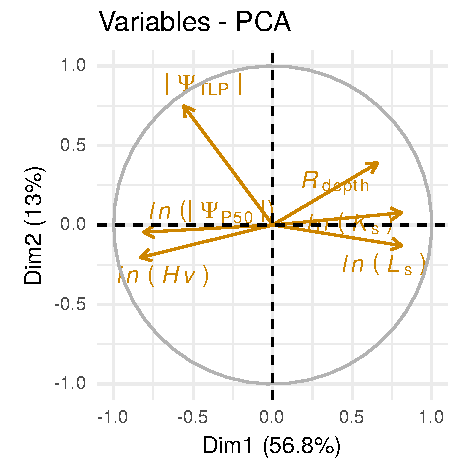
\includegraphics{figure/appendixD/figpca} 

}

\caption{PCA plot of water relations traits using imputations. $ln(|\Psi_{\text{P50}}|)$: logarithm of absolute water potential at 50\% water conductivity loss; $ln(K_{\text{s}})$: logarithm of maximum sapwood water conductivity; $ln(Hv)$: logarithm of Huber value; $|\Psi_{\text{TLP}}|$: absolute water potential at turgor-loss point; $R_{\text{depth}}$: rooting depth; $ln(L_{\text{s}})$: logarithm of individual leaf area.}\label{fig:unnamed-chunk-18}
\end{figure}
\begin{landscape}
\begin{figure}[H]

{\centering 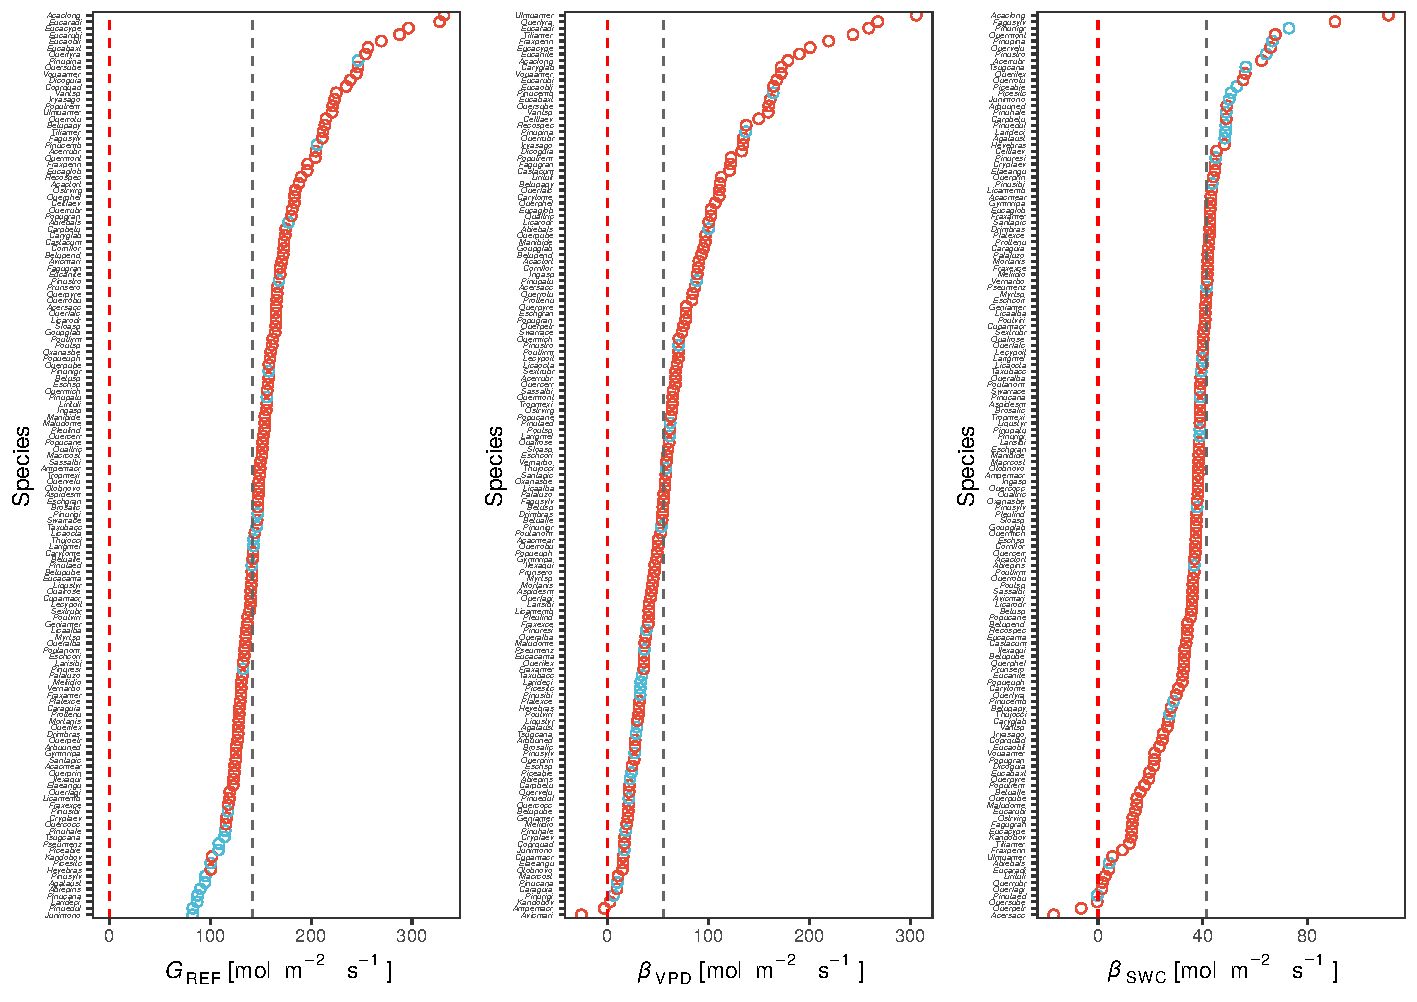
\includegraphics[width=0.9\linewidth]{figure/appendixD/fig17} 

}

\caption{Water use parameters at the species level. Grey dashed lines are the weighted mean of the parameters}\label{fig:spparamplot}
\end{figure}

\end{landscape}
\begin{figure}[H]

{\centering 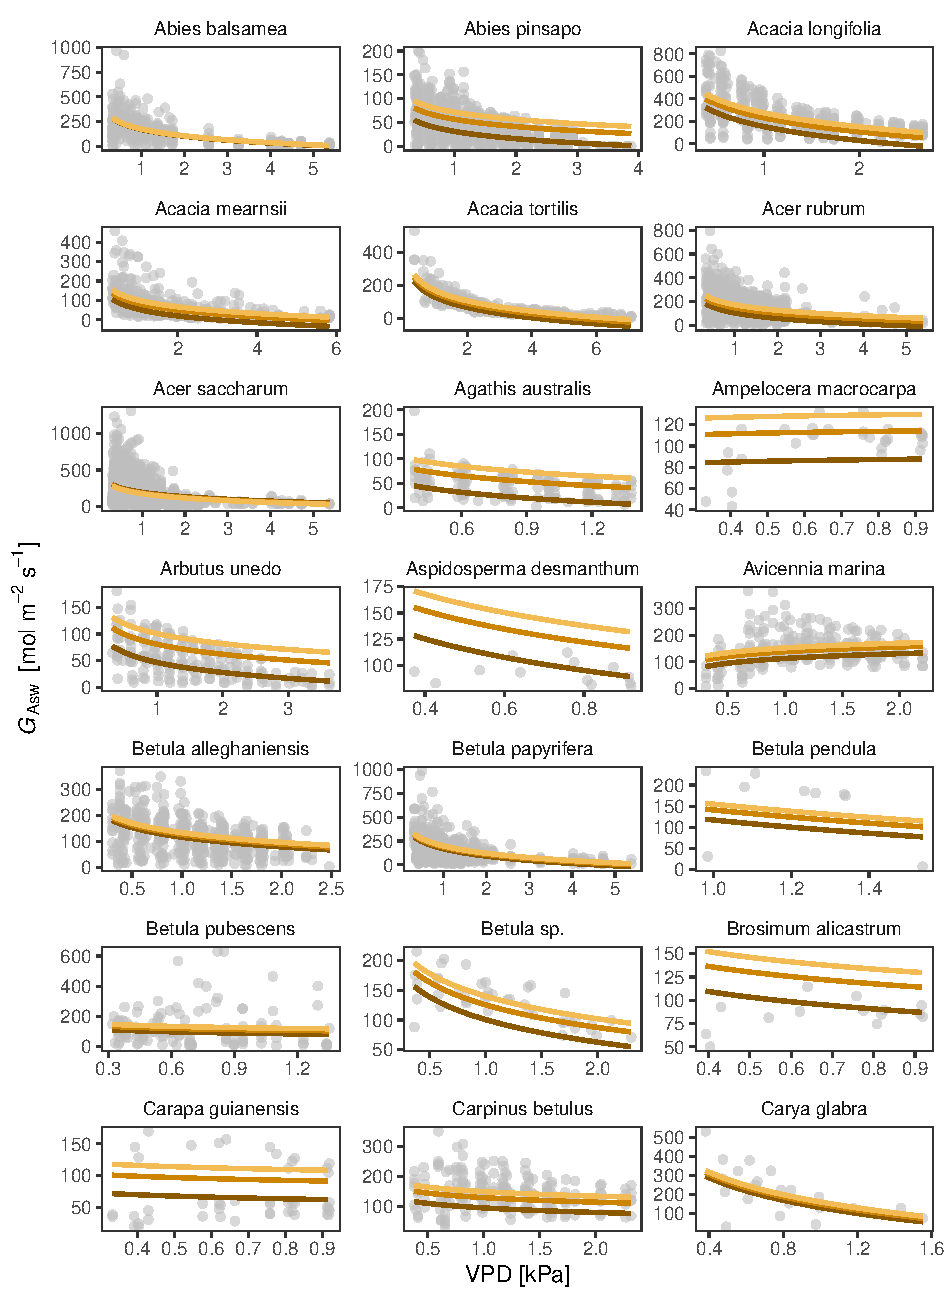
\includegraphics[width=1\linewidth]{figure/appendixD/ggg1} 

}

\end{figure}
\begin{figure}[H]

{\centering 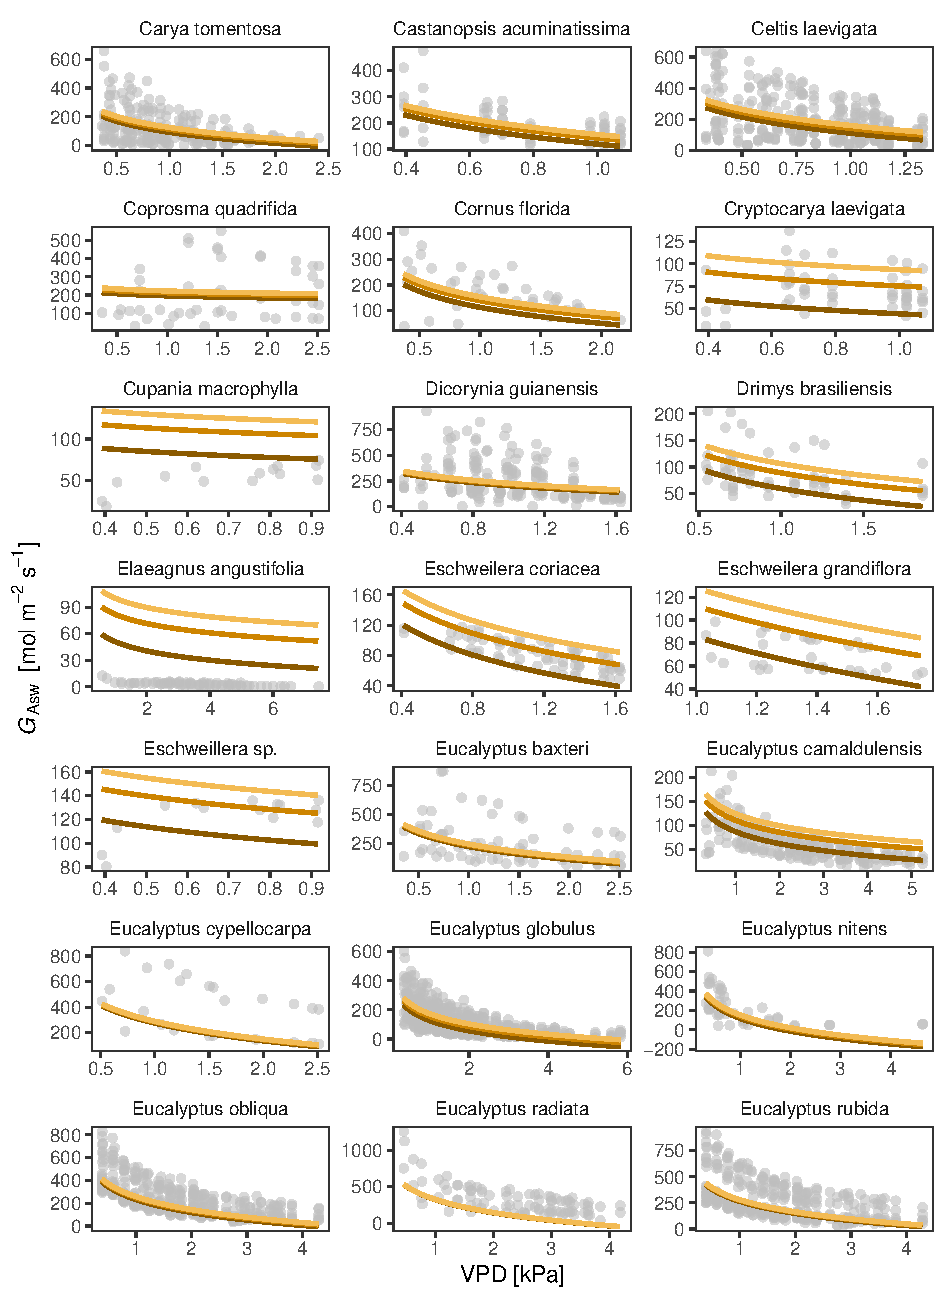
\includegraphics[width=1\linewidth]{figure/appendixD/ggg2} 

}

\end{figure}
\begin{figure}[H]

{\centering 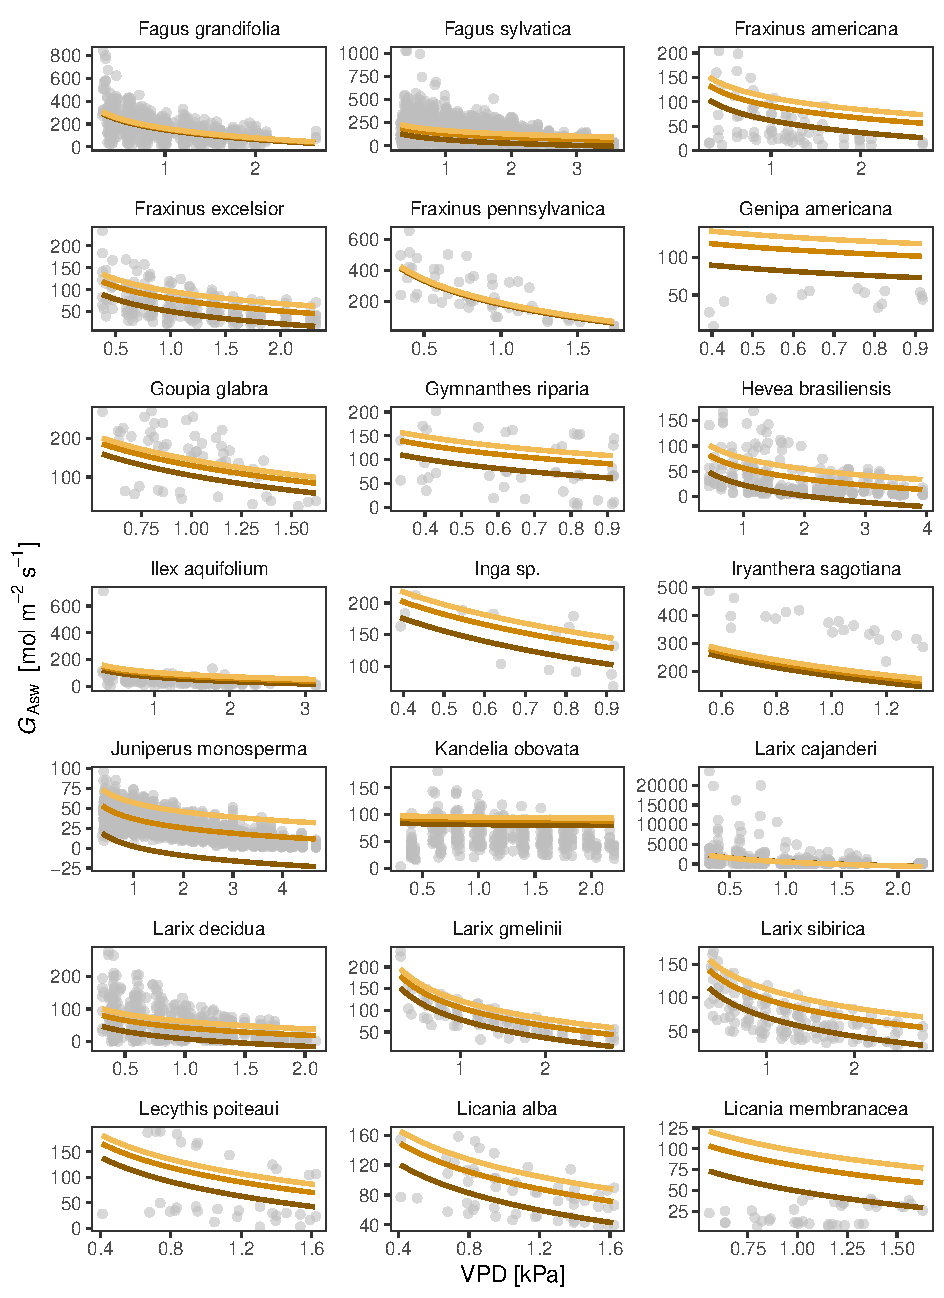
\includegraphics[width=1\linewidth]{figure/appendixD/ggg3} 

}

\end{figure}
\begin{figure}[H]

{\centering 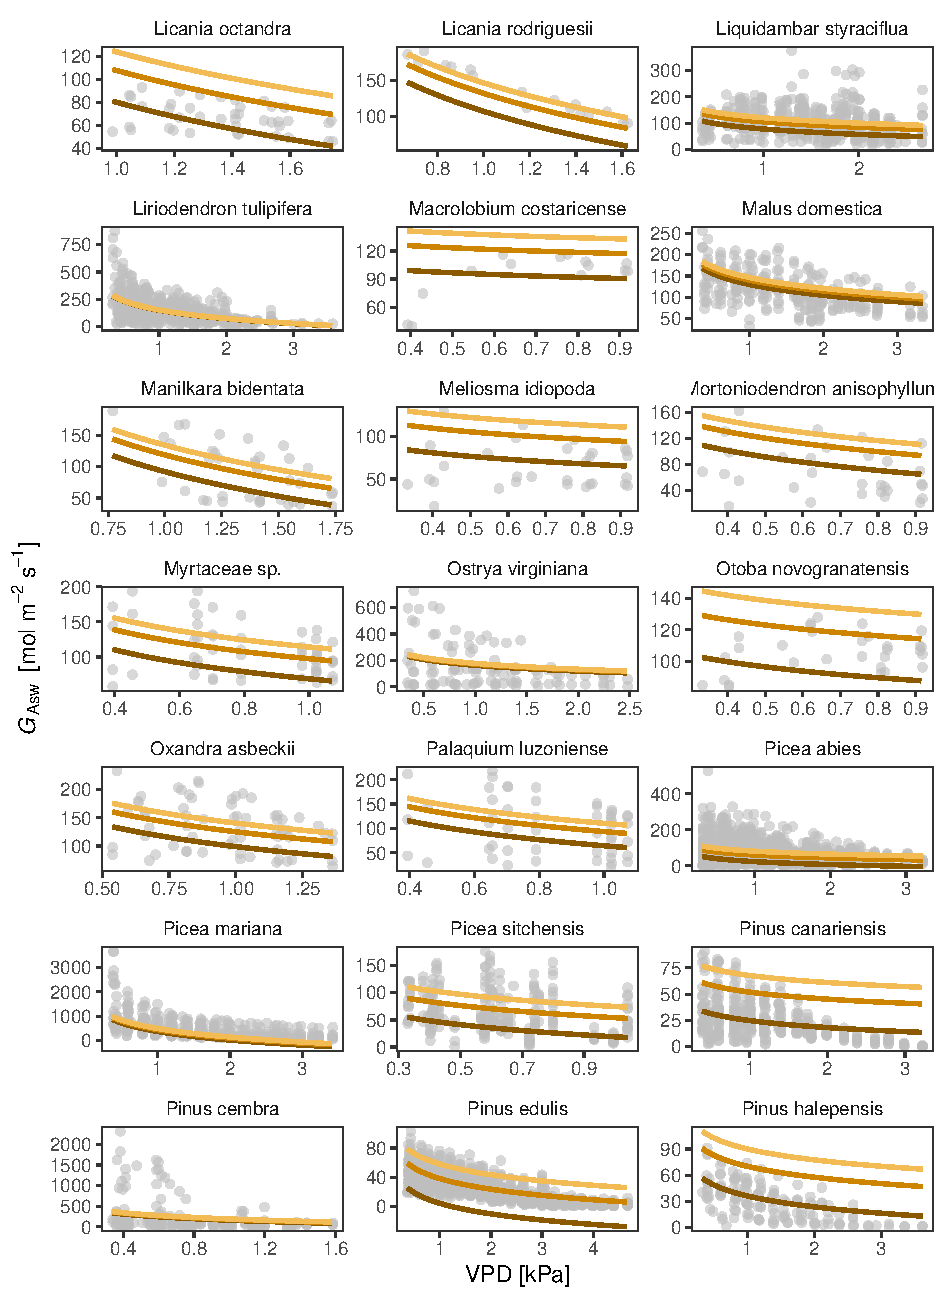
\includegraphics[width=1\linewidth]{figure/appendixD/ggg4} 

}

\end{figure}
\begin{figure}[H]

{\centering 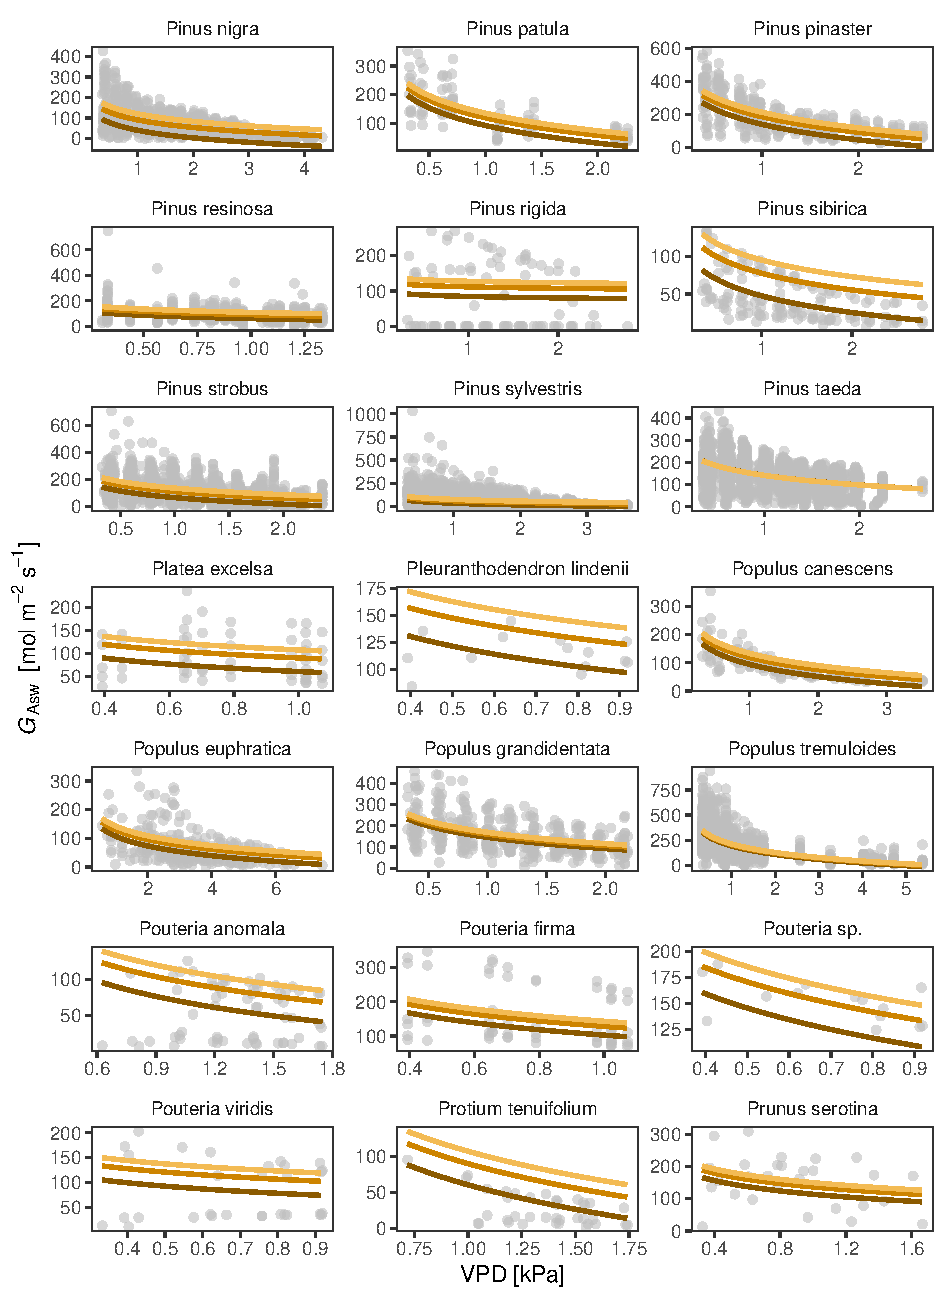
\includegraphics[width=1\linewidth]{figure/appendixD/ggg5} 

}

\end{figure}
\begin{figure}[H]

{\centering 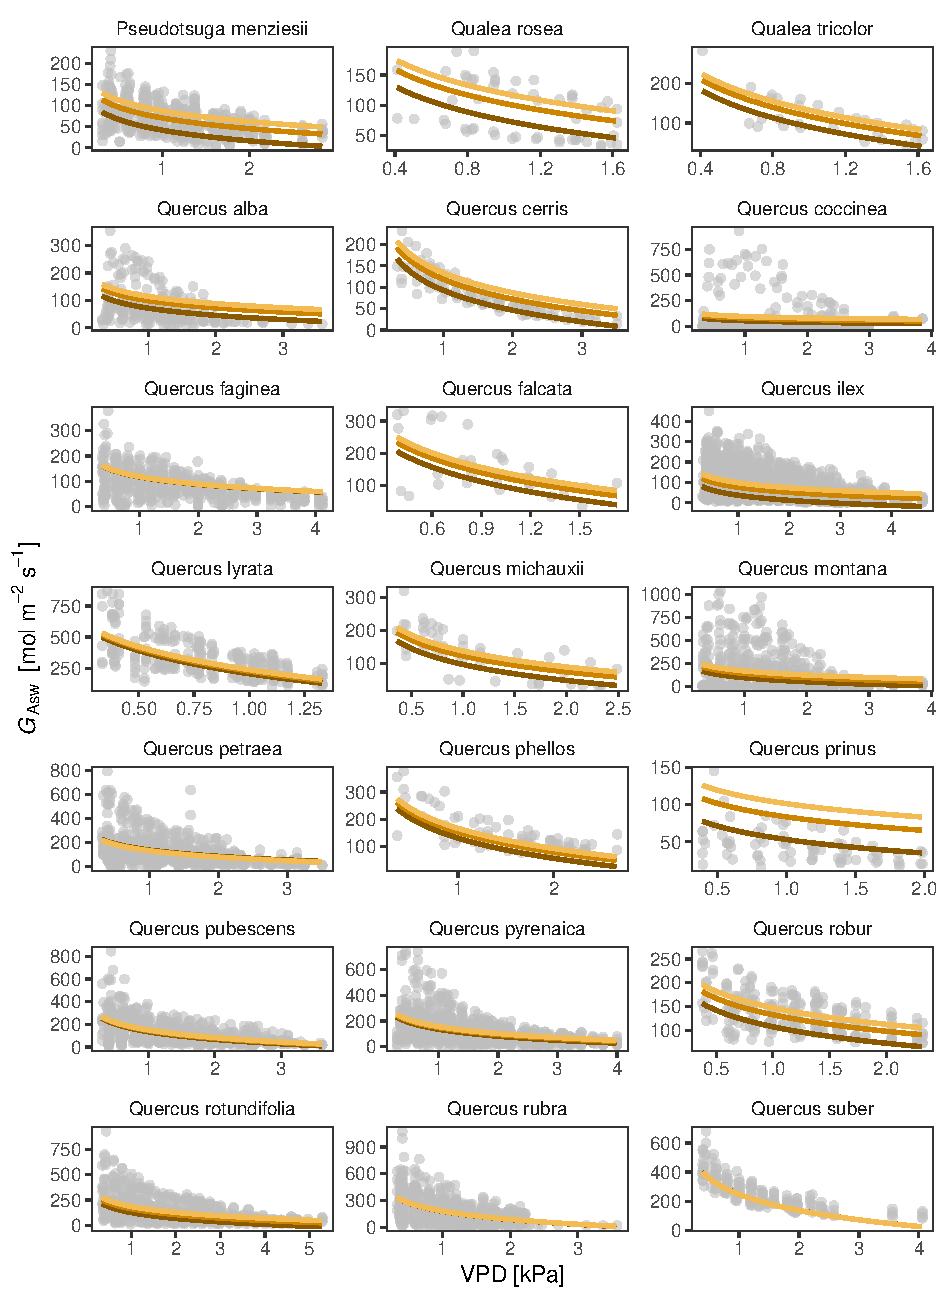
\includegraphics[width=1\linewidth]{figure/appendixD/ggg6} 

}

\end{figure}
\begin{figure}[H]

{\centering 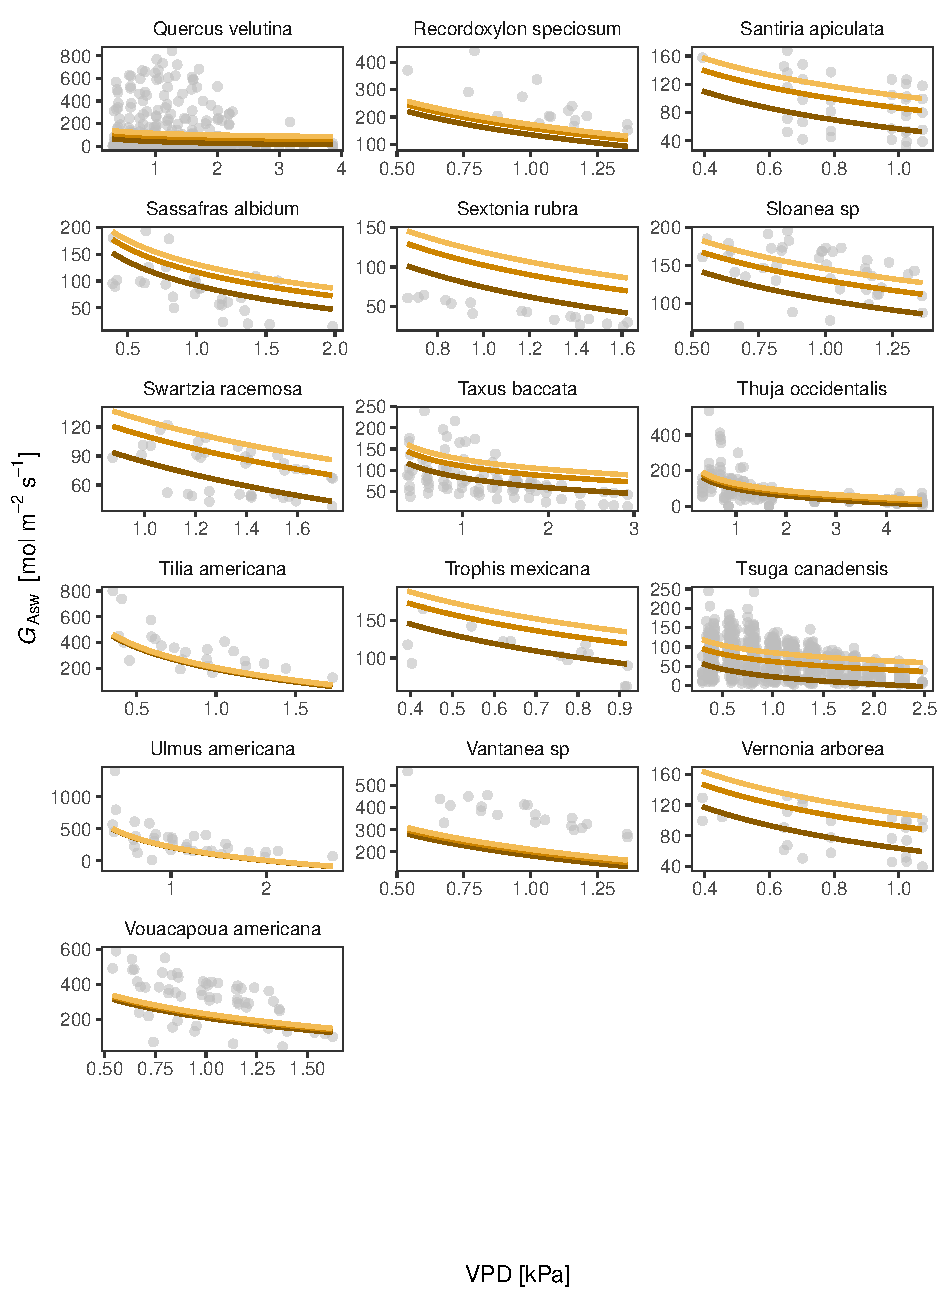
\includegraphics[width=1\linewidth]{figure/appendixD/ggg7} 

}

\caption{Species $G_{Asw}$ responses to VPD. Each species have different curves representing distinct levels of SWC (from dark to light, 0.1, 0.2, 0.3 [$m^3 m^{-3}$]).}\label{fig:unnamed-chunk-25}
\end{figure}
\begin{figure}[H]

{\centering 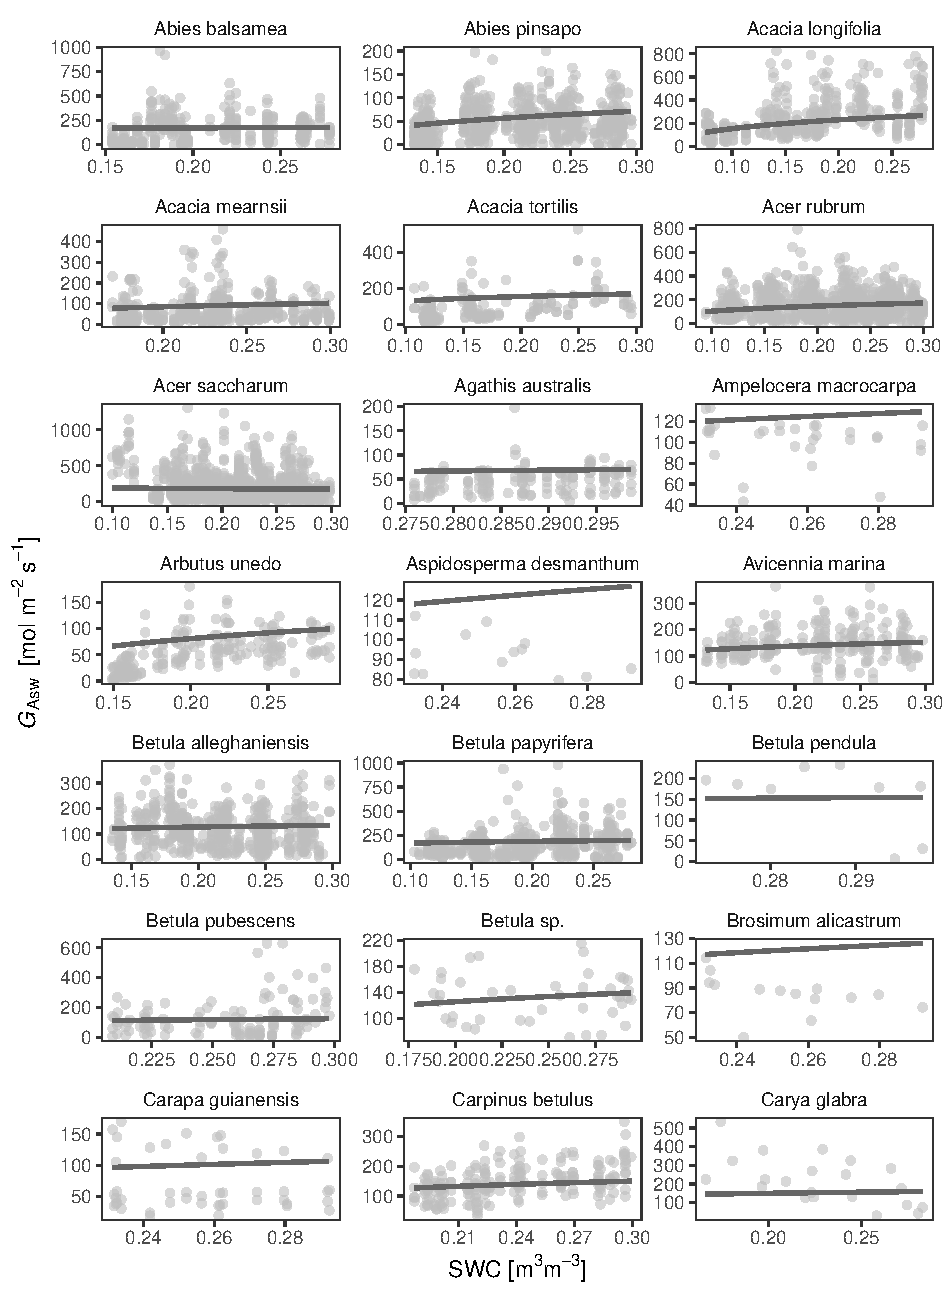
\includegraphics[width=1\linewidth]{figure/appendixD/ggg9} 

}

\end{figure}
\begin{figure}[H]

{\centering 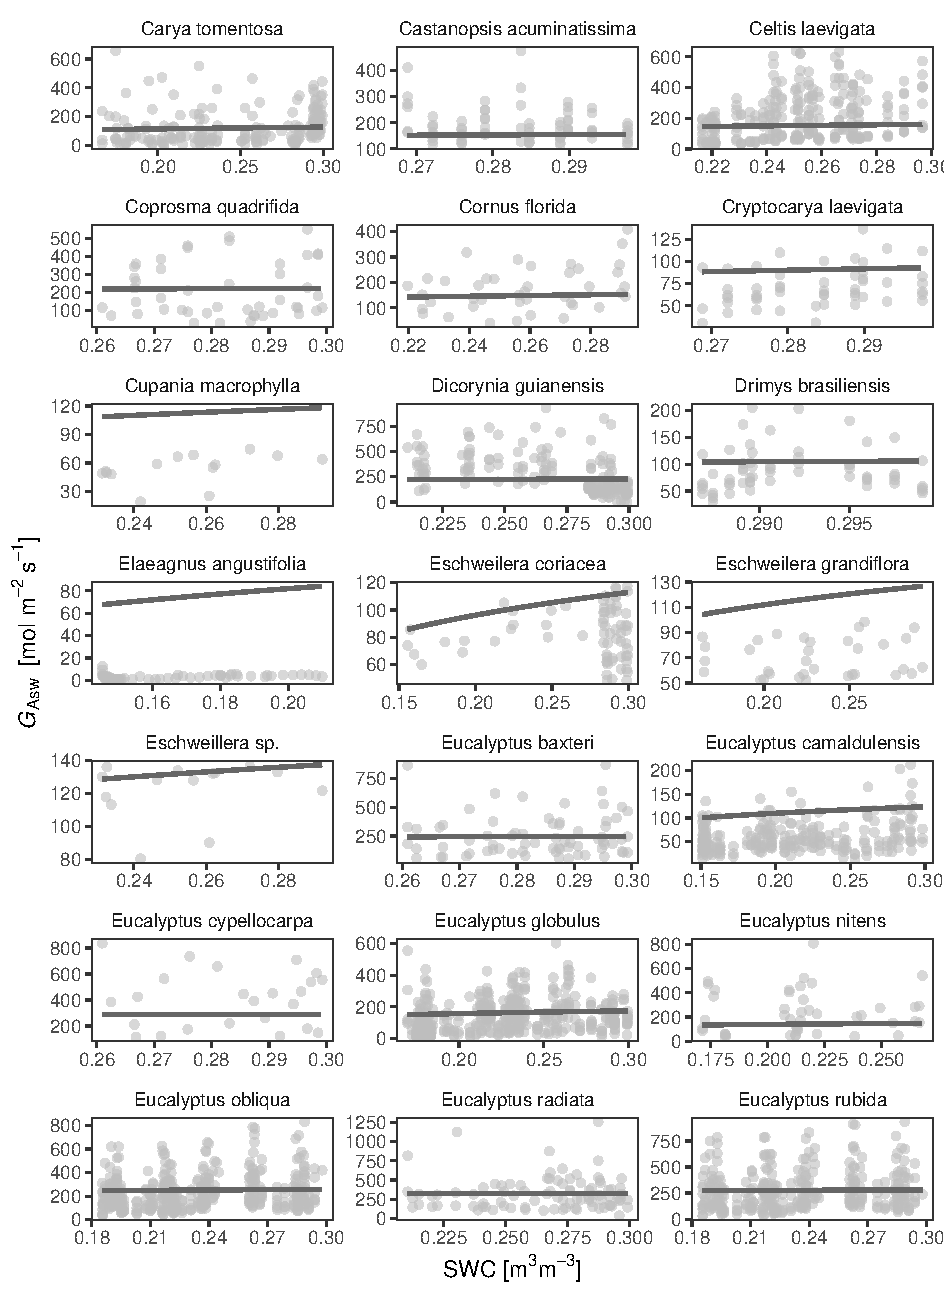
\includegraphics[width=1\linewidth]{figure/appendixD/ggg10} 

}

\end{figure}
\begin{figure}[H]

{\centering 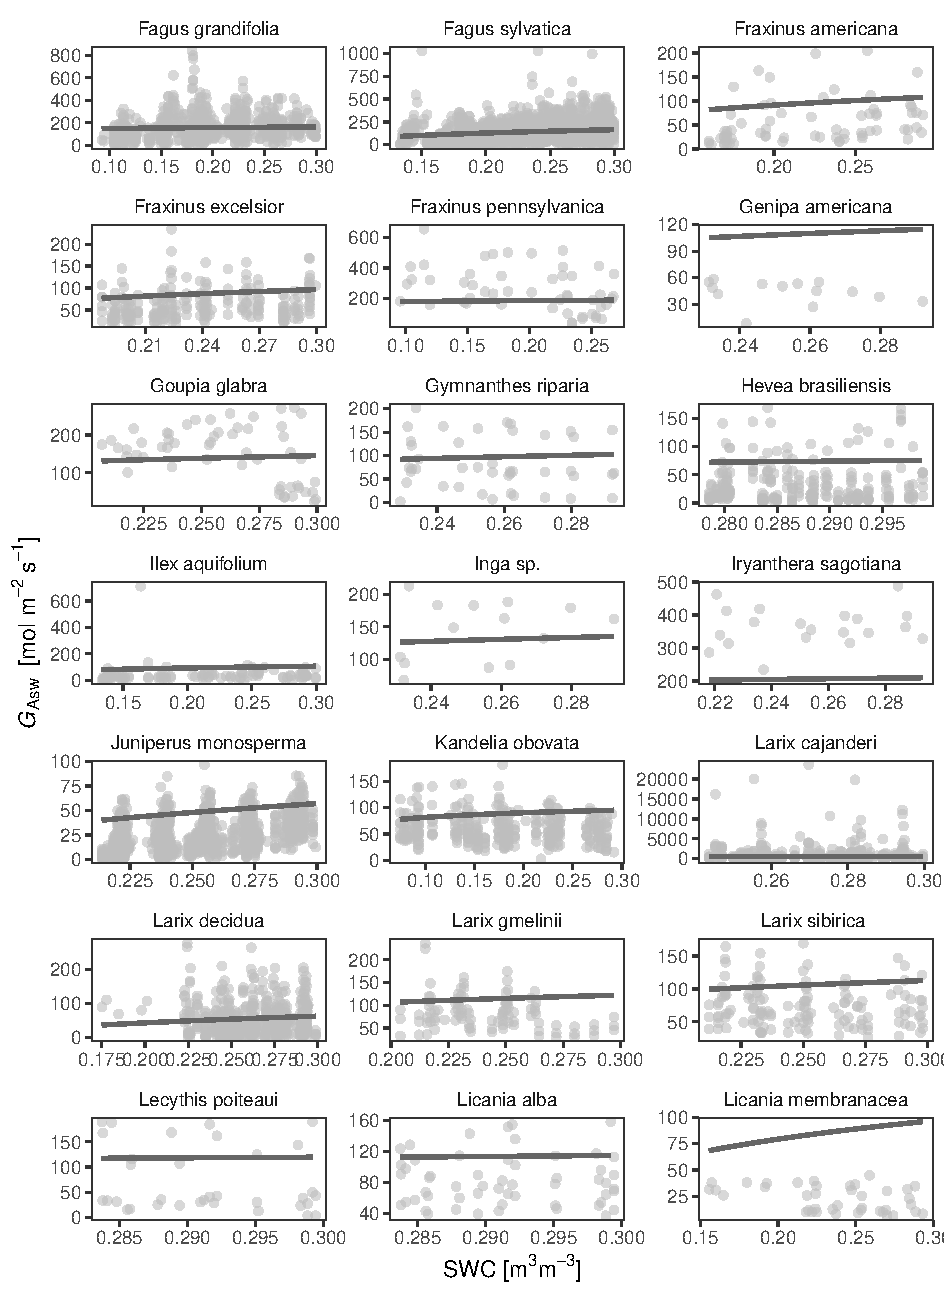
\includegraphics[width=1\linewidth]{figure/appendixD/ggg11} 

}

\end{figure}
\begin{figure}[H]

{\centering 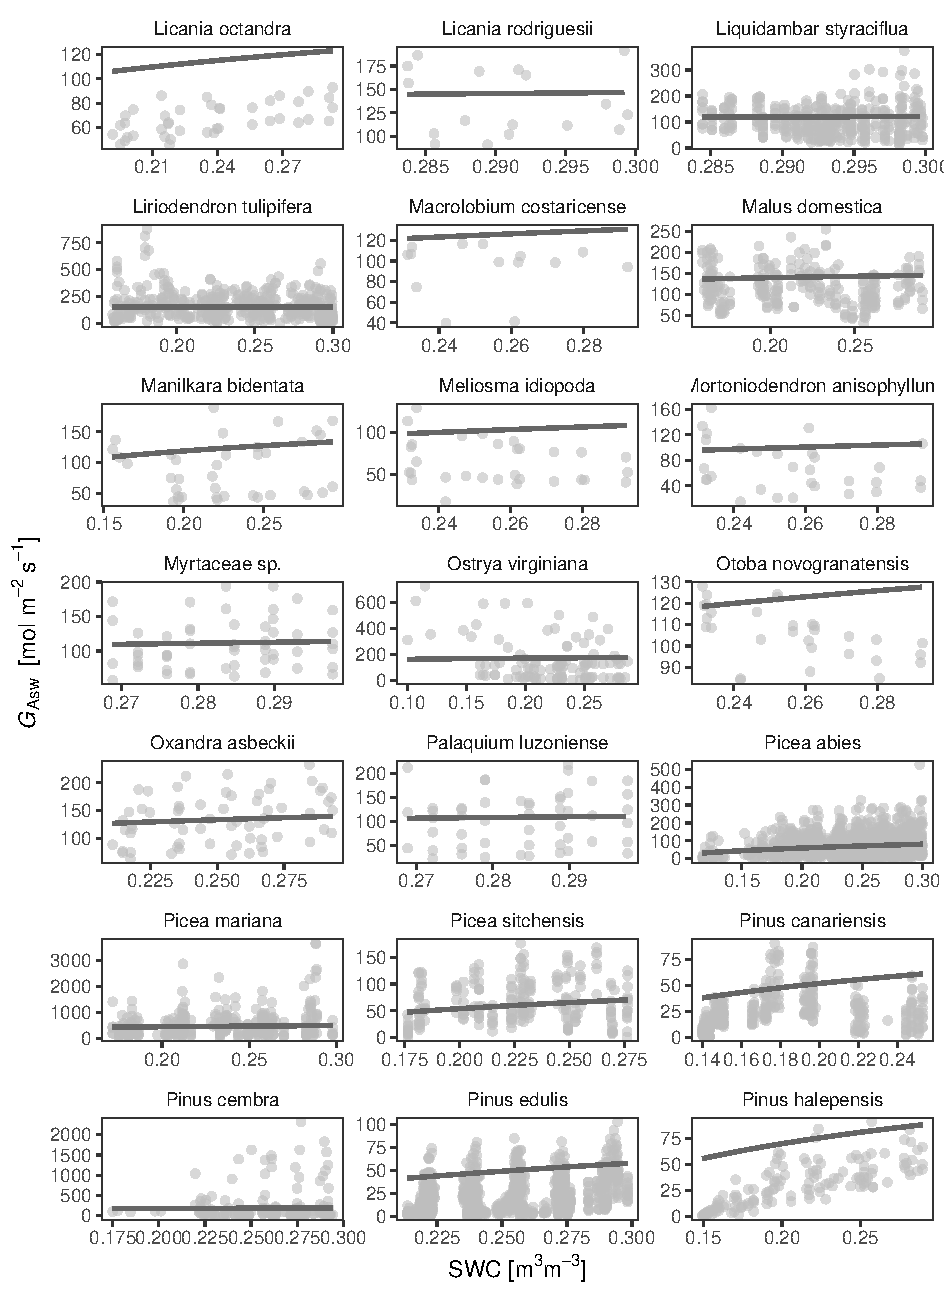
\includegraphics[width=1\linewidth]{figure/appendixD/ggg12} 

}

\end{figure}
\begin{figure}[H]

{\centering 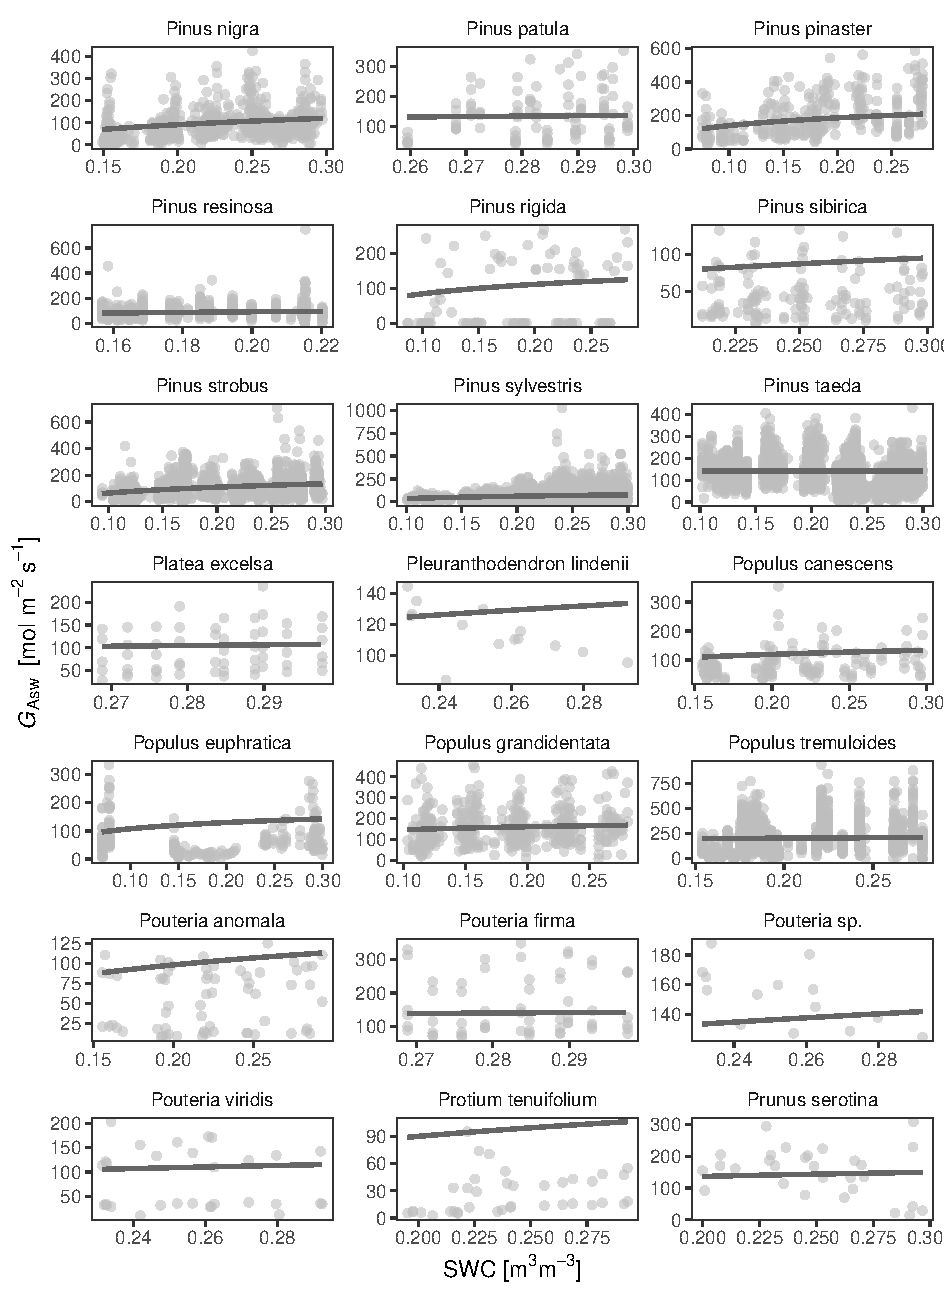
\includegraphics[width=1\linewidth]{figure/appendixD/ggg13} 

}

\end{figure}
\begin{figure}[H]

{\centering 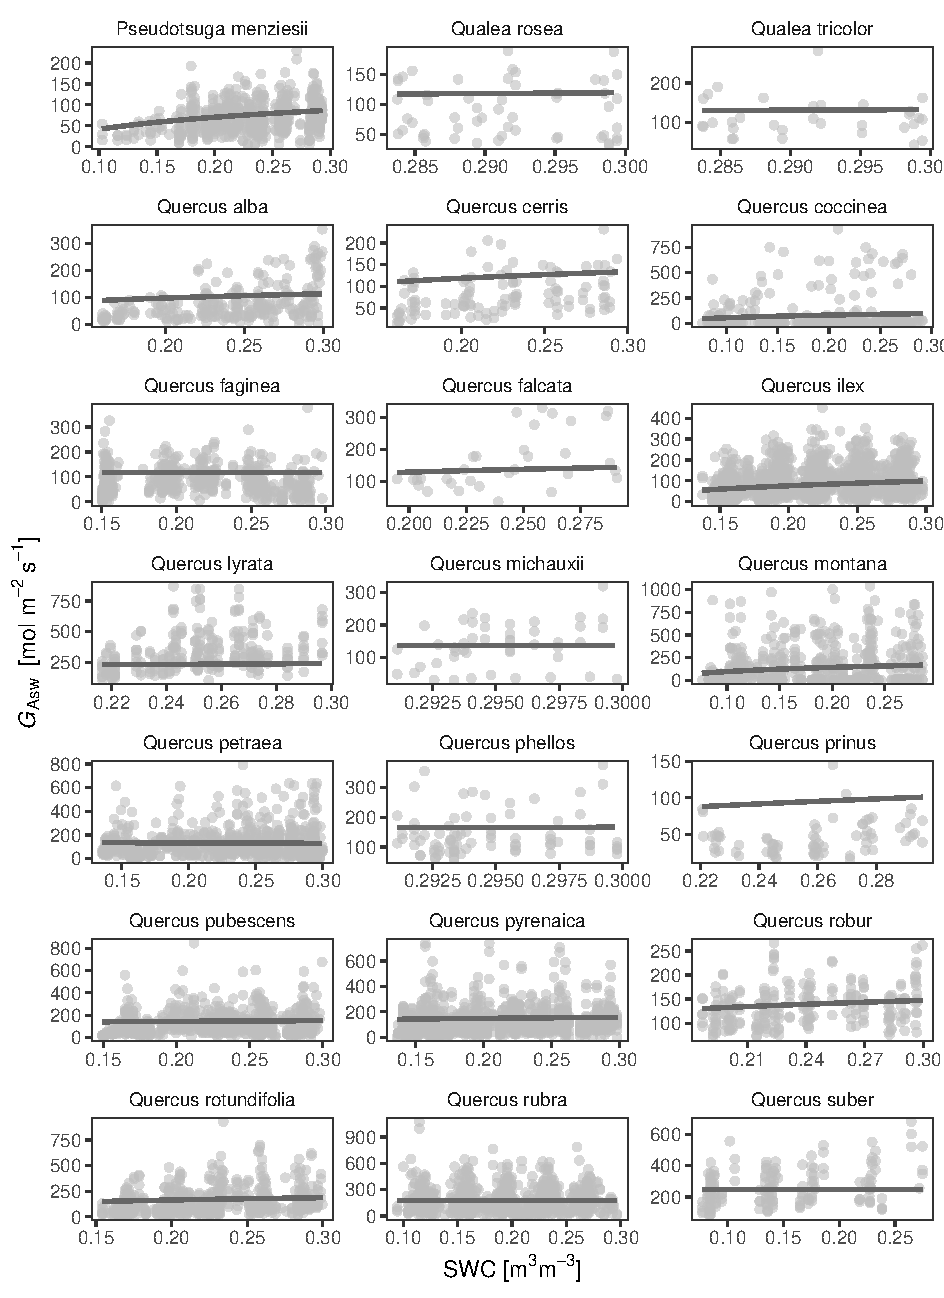
\includegraphics[width=1\linewidth]{figure/appendixD/ggg14} 

}

\end{figure}
\begin{figure}[H]

{\centering 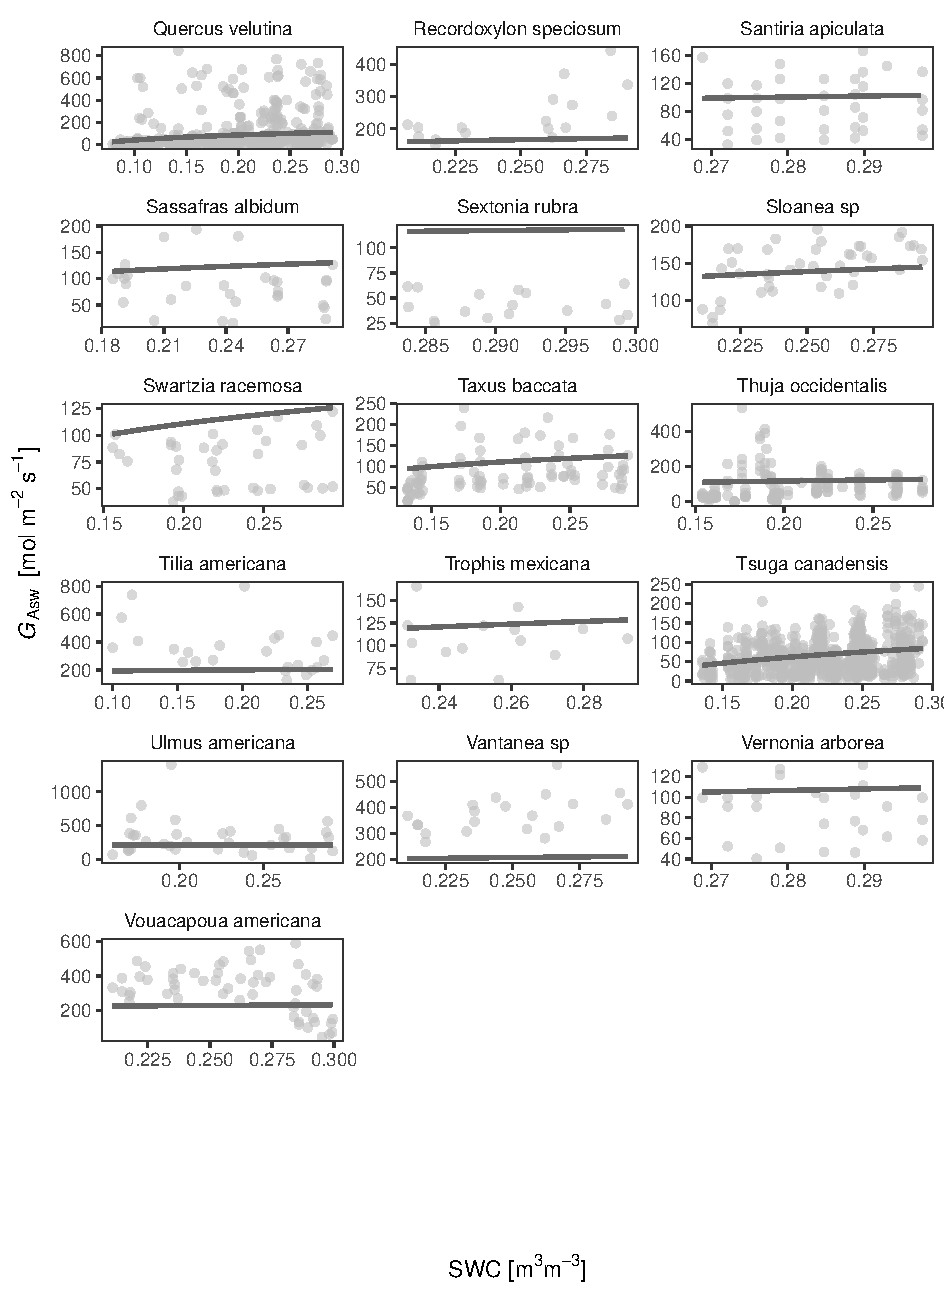
\includegraphics[width=1\linewidth]{figure/appendixD/ggg15} 

}

\caption{Species $G_{Asw}$ responses to SWC. Curves are fitted using a VPD reference level of 1 kPa.}\label{fig:unnamed-chunk-32}
\end{figure}
\begin{figure}[H]

{\centering 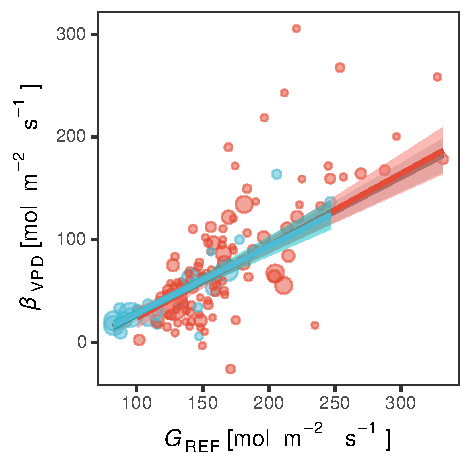
\includegraphics[width=1\linewidth]{figure/appendixD/fig_Gref_b1} 

}

\caption{Scatterplot between $G_{\text{REF}}$ and $\beta_{\text{VPD}}$ parameters. Grey line is global relationship. Blue and red lines are angiosperms and gymnosperms relationships, respectively. Shadow areas are 95\% confidence interval.}\label{fig:corrplot}
\end{figure}
\begin{figure}[H]

{\centering 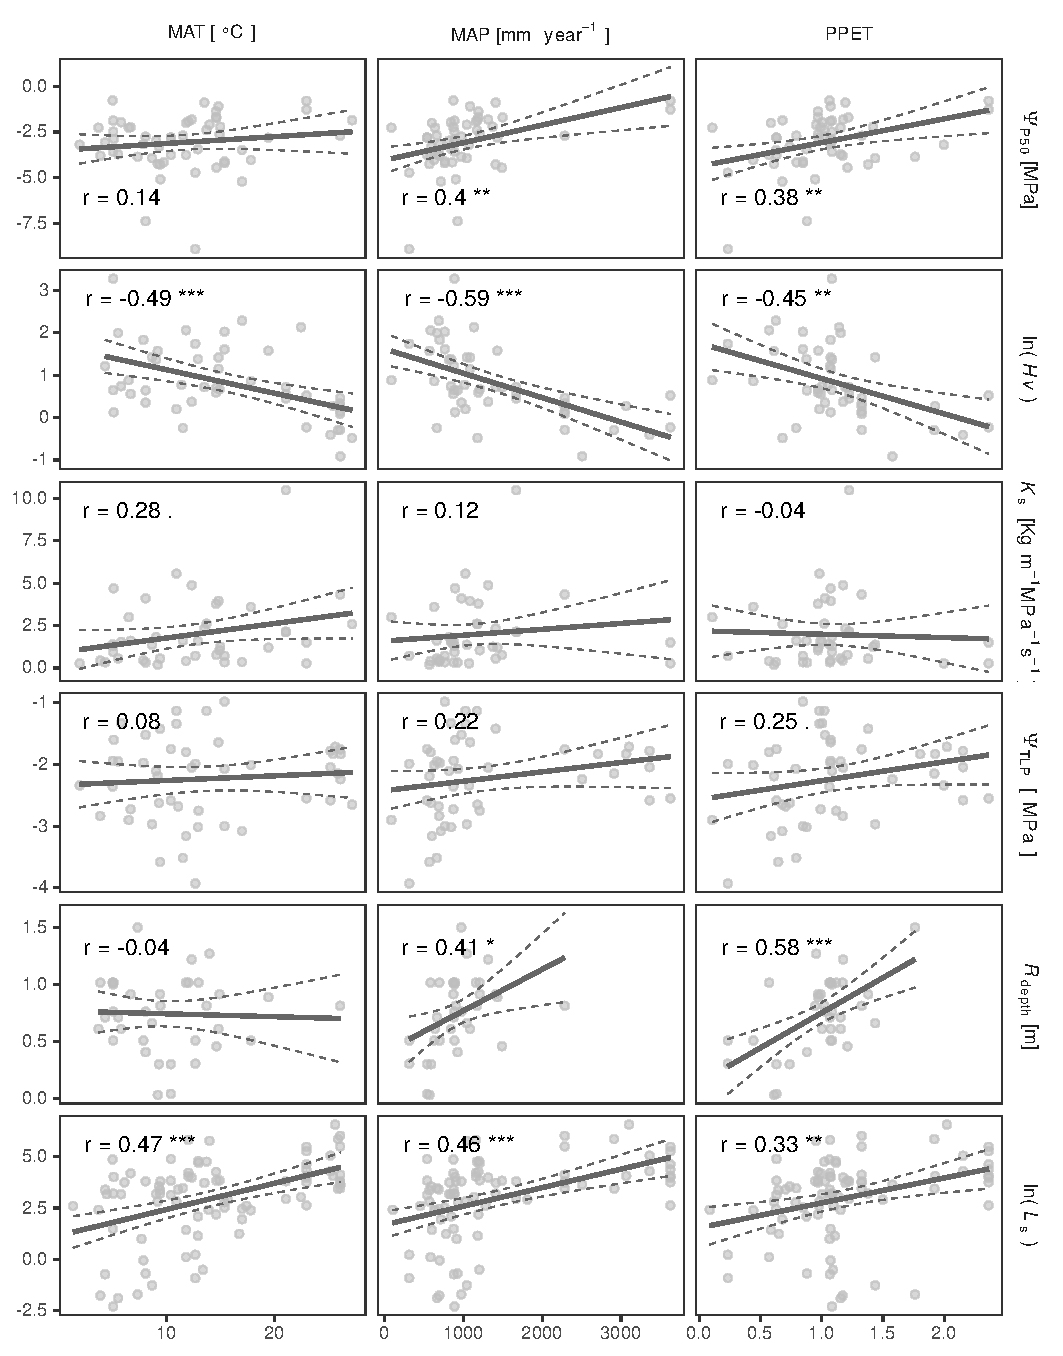
\includegraphics[width=1\linewidth]{figure/appendixD/fig7} 

}

\caption{Species' climatic variables and water relations traits relationships. MAP: mean annual precipitation, MAT: mean annual temperature, PPET: mean annual precipitation over potential evapotranspiration. All climatic variables were calculated as the weighted average of the characteristic plots of the trees of each species, using tree-days as weighting factor.}\label{fig:climatetraitsplot}
\end{figure}
\begin{figure}[H]

{\centering \includegraphics[width=1\linewidth]{figure/appendixD/fig22} 

}

\caption{Species' climatic variables and water use parameters relationships. MAP: mean annual precipitation, MAT: mean annual temperature, PPET: mean annual precipitation over potential evapotranspiration. All climatic variables were calculated as the weighted average of the characteristic plots of the trees of each species, using tree-days as weighting factor.}\label{fig:climateparamplot}
\end{figure}
\begin{figure}[H]

{\centering \includegraphics[width=1\linewidth]{figure/appendixD/figanggym} 

}

\caption{Boxplots of water relations traits for angiosperms and gymnosperms. Statistical significance level is showed as symbols: ., P < 0.1; *, P < 0.05; **, P < 0.01; ***, P < 0.001. Crosses are weighted means of each trait by groups}\label{fig:angiogymnoplotsAOVplot}
\end{figure}
\newpage

\section{Tables D}\label{tables-d}
\begin{table}[H]

\caption{\label{tab:plottreatment}SAPFLUXNET plot treatments included in this study (Poyatos $et$ $al.$ 2020).}
\centering
\begin{tabular}[t]{l}
\toprule
Plot treatment\\
\midrule
\\
None\\
Control\\
control\\
Ambient Control\\
Control - Unthinned\\
natural conditions\\
Reference\\
1Premortality\\
2premortality\\
distructive sampling\\
Girdling early successional\\
Pre-thinning\\
Before thinning\\
Before Thinning\\
non thinned\\
none (periodict thinning every 5-6 years  20 to 25\% of basal area)\\
Radiation Level\\
AMBIENT CO2 FACE rings\\
fertilization at plantation\\
AcaciaMonoculture\\
MixtureEucalyptusAndAcacia\\
EucalyptusMonoculture\\
Pre Irrigation\\
\bottomrule
\end{tabular}
\end{table}
\begingroup\fontsize{4.5}{6.5}\selectfont
\begin{longtable}[t]{>{\em\raggedright\arraybackslash}p{10em}>{\raggedright\arraybackslash}p{4em}>{\raggedright\arraybackslash}p{4em}>{\raggedleft\arraybackslash}p{3em}>{\raggedleft\arraybackslash}p{2em}>{\raggedleft\arraybackslash}p{2em}>{\raggedleft\arraybackslash}p{3em}>{\raggedleft\arraybackslash}p{3em}>{\raggedleft\arraybackslash}p{3em}>{\raggedleft\arraybackslash}p{3em}>{\raggedleft\arraybackslash}p{3em}>{\raggedleft\arraybackslash}p{3em}}
\caption{\label{tab:tabledata}Species resume table. CEP names are Cornell Ecology Programs species names. $\Psi_{\text{P50}}$: water potential at 50\% water conductivity loss [MPa], $K_\text{s}$: maximum sapwood water conductivity[Kg\;$\text{m}^{-1}\;\text{MPa}^{-1}\;\text{s}^{-1}$], $Hv$: Huber value [$\text{cm}^2_{\text{Asw}}\;\text{m}^{-2}_{\text{leaf}\;\text{area}}$], $\Psi_{\text{TLP}}$: water potential at turgor-loss point [MPa], $R_{\text{depth}}$: rooting depth [m], $L_{\text{s}}$: individual leaf area [$\text{cm}^2$].}\\
\toprule
\rotatebox{45}{$\text{Species}$} & \rotatebox{45}{$\text{CEP names}$} & \rotatebox{45}{$\text{Group}$} & \rotatebox{45}{$\# \; \text{tree-days}$} & \rotatebox{45}{$\# \; \text{trees}$} & \rotatebox{45}{$\# \; \text{plots}$} & \rotatebox{45}{$\Psi_{\text{P50}}$} & \rotatebox{45}{$K_{\text{s}}$} & \rotatebox{45}{$\Psi_{\text{TLP}}$} & \rotatebox{45}{$Hv$} & \rotatebox{45}{$R_{\text{depth}}$} & \rotatebox{45}{$L_{\text{s}}$}\\
\midrule
\endfirsthead
\caption[]{\label{tab:tabledata}Species resume table. CEP names are Cornell Ecology Programs species names. $\Psi_{\text{P50}}$: water potential at 50\% water conductivity loss [MPa], $K_\text{s}$: maximum sapwood water conductivity[Kg\;$\text{m}^{-1}\;\text{MPa}^{-1}\;\text{s}^{-1}$], $Hv$: Huber value [$\text{cm}^2_{\text{Asw}}\;\text{m}^{-2}_{\text{leaf}\;\text{area}}$], $\Psi_{\text{TLP}}$: water potential at turgor-loss point [MPa], $R_{\text{depth}}$: rooting depth [m], $L_{\text{s}}$: individual leaf area [$\text{cm}^2$]. \textit{(continued)}}\\
\toprule
\rotatebox{45}{$\text{Species}$} & \rotatebox{45}{$\text{CEP names}$} & \rotatebox{45}{$\text{Group}$} & \rotatebox{45}{$\# \; \text{tree-days}$} & \rotatebox{45}{$\# \; \text{trees}$} & \rotatebox{45}{$\# \; \text{plots}$} & \rotatebox{45}{$\Psi_{\text{P50}}$} & \rotatebox{45}{$K_{\text{s}}$} & \rotatebox{45}{$\Psi_{\text{TLP}}$} & \rotatebox{45}{$Hv$} & \rotatebox{45}{$R_{\text{depth}}$} & \rotatebox{45}{$L_{\text{s}}$}\\
\midrule
\endhead
\
\endfoot
\bottomrule
\endlastfoot
Abies balsamea & Abiebals & Gymnosperms & 855 & 19 & 1 & -2.479 & 1.292 &  & 26.600 & 0.508 & \\
Abies pinsapo & Abiepins & Gymnosperms & 11822 & 22 & 3 & -4.150 &  &  &  &  & \\
Acacia longifolia & Acaclong & Angiosperms & 2130 & 10 & 1 &  &  &  &  &  & 11.715\\
Acacia mearnsii & Acacmear & Angiosperms & 4555 & 23 & 2 &  &  &  & 4.134 &  & \\
Acacia tortilis & Acactort & Angiosperms & 1740 & 3 & 1 &  &  &  &  &  & \\
Acer rubrum & Acerrubr & Angiosperms & 17230 & 49 & 9 & -2.755 & 4.108 & -1.520 & 1.422 & 0.762 & 44.983\\
Acer saccharum & Acersacc & Angiosperms & 10928 & 156 & 8 & -2.873 & 4.695 & -1.600 & 1.134 & 1.016 & 55.675\\
Agathis australis & Agataust & Gymnosperms & 1272 & 6 & 1 & -2.210 & 1.250 &  &  &  & \\
Ampelocera macrocarpa & Ampemacr & Angiosperms & 100 & 2 & 1 &  &  &  &  &  & 103.560\\
Arbutus unedo & Arbuuned & Angiosperms & 1900 & 4 & 1 & -4.198 & 0.714 & -0.980 & 5.017 &  & 12.470\\
Aspidosperma desmanthum & Aspidesm & Angiosperms & 35 & 1 & 1 &  &  &  &  &  & 42.925\\
Avicennia marina & Avicmari & Angiosperms & 828 & 6 & 1 &  &  &  & 8.435 &  & 20.800\\
Betula alleghaniensis & Betualle & Angiosperms & 3750 & 16 & 2 &  &  &  &  &  & 29.938\\
Betula papyrifera & Betupapy & Angiosperms & 3869 & 21 & 2 & -1.966 & 1.538 & -1.330 & 2.096 & 0.610 & 23.942\\
Betula pendula & Betupend & Angiosperms & 9 & 1 & 1 & -2.265 &  &  &  & 0.610 & 11.177\\
Betula pubescens & Betupube & Angiosperms & 397 & 9 & 2 &  &  &  &  &  & 13.510\\
Betula sp. & Betusp & Angiosperms & 204 & 2 & 1 &  &  &  &  &  & \\
Brosimum alicastrum & Brosalic & Angiosperms & 40 & 1 & 1 &  &  &  & 1.685 &  & 58.953\\
Carapa guianensis & Caraguia & Angiosperms & 150 & 3 & 1 & -0.800 & 0.270 &  & 0.793 &  & \\
Carpinus betulus & Carpbetu & Angiosperms & 530 & 5 & 1 & -3.750 &  &  &  &  & 23.160\\
Carya glabra & Caryglab & Angiosperms & 47 & 1 & 1 & -2.100 &  &  &  & 1.270 & 324.425\\
Carya tomentosa & Carytome & Angiosperms & 645 & 10 & 2 &  &  &  &  &  & \\
Castanopsis acuminatissima & Castacum & Angiosperms & 96 & 8 & 1 &  & 10.490 &  & 1.570 &  & 45.000\\
Celtis laevigata & Celtlaev & Angiosperms & 745 & 13 & 2 &  &  &  &  &  & 13.580\\
Coprosma quadrifida & Coprquad & Angiosperms & 57 & 4 & 2 &  &  &  &  &  & 0.600\\
Cornus florida & Cornflor & Angiosperms & 126 & 1 & 1 & -4.442 & 0.768 &  & 2.034 & 0.457 & 46.343\\
Cryptocarya laevigata & Cryplaev & Angiosperms & 72 & 6 & 1 &  & 2.140 &  & 1.750 &  & 19.075\\
Cupania macrophylla & Cupamacr & Angiosperms & 40 & 1 & 1 &  &  &  &  &  & \\
Dicorynia guianensis & Dicoguia & Angiosperms & 596 & 9 & 2 &  &  & -1.712 &  &  & 717.500\\
Drimys brasiliensis & Drimbras & Angiosperms & 90 & 5 & 1 &  &  &  &  &  & 18.420\\
Elaeagnus angustifolia & Elaeangu & Angiosperms & 402 & 2 & 1 &  &  &  &  &  & 11.200\\
Eschweilera coriacea & Eschcori & Angiosperms & 249 & 4 & 2 &  &  & -1.828 & 1.312 &  & 58.654\\
Eschweilera grandiflora & Eschgran & Angiosperms & 378 & 2 & 1 &  &  & -1.754 & 0.746 &  & 62.085\\
Eschweillera sp. & Eschsp & Angiosperms & 40 & 1 & 1 &  &  &  &  &  & \\
Eucalyptus baxteri & Eucabaxt & Angiosperms & 112 & 4 & 2 &  &  &  &  &  & \\
Eucalyptus camaldulensis & Eucacama & Angiosperms & 564 & 3 & 1 & -4.025 & 3.600 & -2.010 & 2.364 & 0.508 & 10.910\\
Eucalyptus cypellocarpa & Eucacype & Angiosperms & 29 & 2 & 2 &  &  &  &  &  & \\
Eucalyptus globulus & Eucaglob & Angiosperms & 4555 & 23 & 2 & -1.100 & 3.950 & -1.640 & 3.155 & 0.610 & \\
Eucalyptus nitens & Eucanite & Angiosperms & 378 & 7 & 1 &  &  &  & 2.163 &  & \\
Eucalyptus obliqua & Eucaobli & Angiosperms & 2466 & 6 & 1 &  &  & -1.340 &  &  & 16.790\\
Eucalyptus radiata & Eucaradi & Angiosperms & 170 & 2 & 1 &  &  &  &  &  & \\
Eucalyptus rubida & Eucarubi & Angiosperms & 2055 & 5 & 1 &  & 5.560 & -1.130 & 1.222 &  & \\
Fagus grandifolia & Fagugran & Angiosperms & 6815 & 32 & 3 & -5.080 &  &  &  & 0.813 & 45.167\\
Fagus sylvatica & Fagusylv & Angiosperms & 15075 & 93 & 12 & -2.972 & 1.830 & -2.107 & 3.934 &  & 24.030\\
Fraxinus americana & Fraxamer & Angiosperms & 378 & 2 & 1 & -1.920 &  &  &  & 1.016 & 339.552\\
Fraxinus excelsior & Fraxexce & Angiosperms & 636 & 6 & 1 & -2.805 &  & -1.750 &  & 0.040 & 133.800\\
Fraxinus pennsylvanica & Fraxpenn & Angiosperms & 178 & 2 & 1 & -0.777 & 1.397 & -2.360 &  & 1.016 & \\
Genipa americana & Geniamer & Angiosperms & 40 & 1 & 1 & -1.270 & 1.500 & -2.550 &  &  & 242.210\\
Goupia glabra & Goupglab & Angiosperms & 172 & 3 & 3 &  &  &  &  &  & 31.288\\
Gymnanthes riparia & Gymnripa & Angiosperms & 150 & 3 & 1 &  &  &  &  &  & \\
Hevea brasiliensis & Hevebras & Angiosperms & 1302 & 6 & 1 & -1.859 & 2.582 & -2.650 & 0.618 &  & \\
Ilex aquifolium & Ilexaqui & Angiosperms & 567 & 3 & 1 & -4.241 & 0.186 & -2.190 & 4.825 & 0.030 & 16.770\\
Inga sp. & Ingasp & Angiosperms & 40 & 1 & 1 &  &  &  &  &  & \\
Iryanthera sagotiana & Iryasago & Angiosperms & 72 & 1 & 1 &  &  & -1.830 &  &  & \\
Juniperus monosperma & Junimono & Gymnosperms & 23650 & 15 & 3 & -8.882 & 0.710 & -3.930 & 5.700 & 0.305 & 0.400\\
Kandelia obovata & Kandobov & Angiosperms & 2584 & 8 & 1 &  &  &  &  &  & \\
Larix decidua & Larideci & Gymnosperms & 3127 & 23 & 5 & -3.791 & 0.434 & -2.835 &  & 1.016 & 0.170\\
Larix gmelinii & Larigmel & Gymnosperms & 303 & 3 & 1 &  &  &  &  &  & \\
Larix sibirica & Larisibi & Angiosperms & 516 & 3 & 1 &  &  &  &  &  & \\
Lecythis poiteaui & Lecypoit & Angiosperms & 90 & 2 & 1 &  &  & -2.581 &  &  & \\
Licania alba & Licaalba & Angiosperms & 141 & 3 & 1 &  &  & -2.044 & 0.664 &  & 157.435\\
Licania membranacea & Licamemb & Angiosperms & 217 & 2 & 2 &  &  & -2.239 & 0.401 &  & 38.313\\
Licania octandra & Licaocta & Angiosperms & 256 & 2 & 1 &  &  &  & 1.088 &  & 32.005\\
Licania rodriguesii & Licarodr & Angiosperms & 34 & 1 & 1 &  &  &  &  &  & \\
Liquidambar styraciflua & Liqustyr & Angiosperms & 742 & 23 & 3 & -2.622 & 1.042 &  & 1.949 & 0.914 & 47.104\\
Liriodendron tulipifera & Lirituli & Angiosperms & 2246 & 27 & 7 & -2.390 & 2.610 & -1.130 &  & 0.813 & 116.933\\
Macrolobium costaricense & Macrcost & Angiosperms & 40 & 1 & 1 &  &  &  &  &  & 79.840\\
Malus domestica & Maludome & Angiosperms & 1175 & 5 & 2 &  &  & -2.070 &  &  & 16.200\\
Manilkara bidentata & Manibide & Angiosperms & 500 & 2 & 1 & -2.700 & 4.333 &  & 1.309 & 0.813 & 45.229\\
Meliosma idiopoda & Meliidio & Angiosperms & 100 & 2 & 1 &  &  &  &  &  & \\
Mortoniodendron anisophyllum & Mortanis & Angiosperms & 100 & 2 & 1 &  &  &  &  &  & \\
Myrtaceae sp. & Myrtsp & Angiosperms & 72 & 6 & 1 &  &  &  &  &  & \\
Ostrya virginiana & Ostrvirg & Angiosperms & 549 & 3 & 2 &  &  &  &  &  & 23.994\\
Otoba novogranatensis & Otobnovo & Angiosperms & 100 & 2 & 1 &  &  &  &  &  & 196.140\\
Oxandra asbeckii & Oxanasbe & Angiosperms & 263 & 3 & 2 &  &  &  &  &  & \\
Palaquium luzoniense & Palaluzo & Angiosperms & 72 & 6 & 1 &  &  &  &  &  & \\
Picea abies & Piceabie & Gymnosperms & 11873 & 109 & 11 & -3.714 & 0.558 & -1.950 & 7.375 & 0.711 & 0.150\\
Picea sitchensis & Picesitc & Gymnosperms & 990 & 15 & 1 & -3.850 &  &  &  & 1.500 & 0.180\\
Pinus canariensis & Pinucana & Gymnosperms & 4890 & 10 & 1 &  &  &  &  &  & \\
Pinus cembra & Pinucemb & Gymnosperms & 1151 & 14 & 5 & -3.192 & 0.267 & -2.340 &  &  & \\
Pinus edulis & Pinuedul & Gymnosperms & 23715 & 15 & 3 & -4.718 &  & -1.990 &  & 0.508 & 1.250\\
Pinus halepensis & Pinuhale & Gymnosperms & 1329 & 3 & 1 & -4.105 & 0.335 & -3.000 & 7.590 &  & \\
Pinus nigra & Pinunigr & Gymnosperms & 11246 & 15 & 3 & -3.753 & 0.407 & -1.800 & 7.860 & 1.016 & 1.110\\
Pinus patula & Pinupatu & Gymnosperms & 152 & 8 & 1 &  &  &  &  &  & \\
Pinus pinaster & Pinupina & Gymnosperms & 2130 & 10 & 1 & -3.489 & 0.352 &  & 9.870 &  & \\
Pinus resinosa & Pinuresi & Gymnosperms & 1176 & 42 & 1 &  &  & -1.940 &  & 1.016 & 4.400\\
Pinus rigida & Pinurigi & Gymnosperms & 489 & 2 & 2 &  &  &  &  &  & 3.150\\
Pinus sibirica & Pinusibi & Gymnosperms & 516 & 3 & 1 &  &  &  &  &  & \\
Pinus strobus & Pinustro & Gymnosperms & 32538 & 60 & 4 &  &  &  &  &  & 2.700\\
Pinus sylvestris & Pinusylv & Gymnosperms & 42463 & 215 & 21 & -3.163 & 0.448 & -1.975 & 6.257 & 0.508 & 0.947\\
Pinus taeda & Pinutaed & Gymnosperms & 24380 & 97 & 4 & -2.810 & 1.197 &  & 4.848 & 0.889 & \\
Platea excelsa & Platexce & Angiosperms & 72 & 6 & 1 &  &  &  &  &  & \\
Pleuranthodendron lindenii & Pleulind & Angiosperms & 40 & 1 & 1 &  &  &  &  &  & 53.633\\
Populus canescens & Popucane & Angiosperms & 597 & 3 & 1 &  &  &  &  &  & \\
Populus euphratica & Popueuph & Angiosperms & 841 & 9 & 3 & -2.264 & 2.998 & -2.900 & 2.420 &  & \\
Populus grandidentata & Popugran & Angiosperms & 6888 & 12 & 1 &  &  &  &  &  & 42.608\\
Populus tremuloides & Poputrem & Angiosperms & 4455 & 99 & 1 & -1.876 & 0.934 &  & 1.910 & 1.000 & 24.690\\
Pouteria anomala & Poutanom & Angiosperms & 912 & 3 & 1 &  &  &  & 1.392 &  & 42.295\\
Pouteria firma & Poutfirm & Angiosperms & 72 & 6 & 1 &  &  &  &  &  & \\
Pouteria sp. & Poutsp & Angiosperms & 40 & 1 & 1 &  &  &  &  &  & \\
Pouteria viridis & Poutviri & Angiosperms & 100 & 2 & 1 &  &  &  &  &  & \\
Protium tenuifolium & Prottenu & Angiosperms & 242 & 2 & 1 &  &  &  & 1.587 &  & 413.810\\
Prunus serotina & Prunsero & Angiosperms & 100 & 1 & 1 & -4.270 & 0.550 & -1.420 &  & 0.914 & 24.759\\
Pseudotsuga menziesii & Pseumenz & Gymnosperms & 2985 & 18 & 3 & -3.926 & 1.366 & -2.970 & 4.153 & 0.660 & 0.280\\
Qualea rosea & Qualrose & Angiosperms & 141 & 3 & 1 &  &  & -1.779 &  &  & \\
Qualea tricolor & Qualtric & Angiosperms & 78 & 2 & 1 &  &  &  &  &  & \\
Quercus alba & Queralba & Angiosperms & 1094 & 9 & 5 & -1.818 & 4.877 & -2.050 & 1.454 & 1.219 & 54.302\\
Quercus cerris & Quercerr & Angiosperms & 284 & 2 & 1 &  &  & -3.580 &  &  & 29.190\\
Quercus coccinea & Quercocc & Angiosperms & 5343 & 11 & 3 &  &  &  &  &  & 121.678\\
Quercus faginea & Querfagi & Angiosperms & 6784 & 10 & 2 & -2.002 &  & -3.160 &  &  & 4.210\\
Quercus falcata & Querfalc & Angiosperms & 134 & 1 & 1 & -0.893 & 2.323 &  & 2.057 &  & 41.635\\
Quercus ilex & Querilex & Angiosperms & 65295 & 62 & 6 & -3.438 & 1.595 & -3.015 & 3.980 &  & 8.078\\
Quercus lyrata & Querlyra & Angiosperms & 745 & 13 & 2 &  &  &  &  &  & \\
Quercus michauxii & Quermich & Angiosperms & 132 & 4 & 1 & -1.700 &  &  &  &  & 71.498\\
Quercus montana & Quermont & Angiosperms & 5488 & 14 & 2 &  &  &  &  &  & \\
Quercus petraea & Querpetr & Angiosperms & 4617 & 29 & 5 & -3.294 &  & -2.624 &  & 0.300 & 35.000\\
Quercus phellos & Querphel & Angiosperms & 185 & 5 & 1 & -1.375 & 3.787 &  & 1.806 &  & 8.935\\
Quercus prinus & Querprin & Angiosperms & 316 & 2 & 1 & -1.700 &  &  &  &  & \\
Quercus pubescens & Querpube & Angiosperms & 6505 & 19 & 2 & -2.696 & 1.612 & -3.515 & 0.782 &  & 32.200\\
Quercus pyrenaica & Querpyre & Angiosperms & 6680 & 32 & 2 &  &  & -2.680 &  &  & 30.260\\
Quercus robur & Querrobu & Angiosperms & 636 & 6 & 1 & -2.802 &  & -2.583 &  & 0.300 & 46.537\\
Quercus rotundifolia & Querrotu & Angiosperms & 4796 & 10 & 2 &  &  &  &  &  & 3.460\\
Quercus rubra & Querrubr & Angiosperms & 15185 & 32 & 6 & -2.237 & 1.602 & -2.725 & 1.746 & 0.914 & 66.641\\
Quercus suber & Quersube & Angiosperms & 1816 & 4 & 1 & -5.200 &  & -3.080 &  &  & 7.030\\
Quercus velutina & Quervelu & Angiosperms & 5132 & 16 & 3 &  &  & -2.750 &  & 1.016 & 110.450\\
Recordoxylon speciosum & Recospec & Angiosperms & 41 & 1 & 1 &  &  &  &  &  & \\
Santiria apiculata & Santapic & Angiosperms & 55 & 5 & 1 &  &  &  &  &  & \\
Sassafras albidum & Sassalbi & Angiosperms & 117 & 1 & 1 &  &  &  &  &  & 68.080\\
Sextonia rubra & Sextrubr & Angiosperms & 34 & 1 & 1 &  &  &  &  &  & 74.000\\
Sloanea sp & Sloasp & Angiosperms & 156 & 2 & 2 &  &  &  &  &  & \\
Swartzia racemosa & Swarrace & Angiosperms & 476 & 2 & 1 &  &  &  & 1.156 &  & 246.450\\
Taxus baccata & Taxubacc & Gymnosperms & 922 & 2 & 1 & -7.360 & 0.320 &  & 1.900 & 0.406 & 0.500\\
Thuja occidentalis & Thujocci & Gymnosperms & 340 & 10 & 1 & -3.570 &  &  &  & 0.762 & 0.100\\
Tilia americana & Tiliamer & Angiosperms & 72 & 1 & 1 &  &  &  &  &  & 130.715\\
Trophis mexicana & Tropmexi & Angiosperms & 40 & 1 & 1 &  &  &  &  &  & 13.880\\
Tsuga canadensis & Tsugcana & Gymnosperms & 5739 & 24 & 2 & -3.070 & 0.329 &  & 3.362 & 0.711 & 0.480\\
Ulmus americana & Ulmuamer & Angiosperms & 133 & 1 & 1 &  &  &  &  &  & 56.993\\
Vantanea sp & Vantsp & Angiosperms & 69 & 1 & 1 &  &  &  &  &  & \\
Vernonia arborea & Vernarbo & Angiosperms & 36 & 3 & 1 &  & 2.110 &  & 2.060 &  & \\
Vouacapoua americana & Vouaamer & Angiosperms & 178 & 3 & 3 &  &  & -2.147 & 0.744 &  & 353.583\\*
\end{longtable}
\endgroup{}

\newpage
\begin{table}

\caption{\label{tab:tab1}Results of the linear models relating water use parameters calculated using $G'_{Asw}$ to water relations traits. Parameters are explained by individual traits using simple linear models with number of species-days as weighting factor.}
\centering
\resizebox{\linewidth}{!}{
\begin{tabular}[t]{llrllr}
\toprule
Parameter & Trait & $\text{N}\;\text{Species}$ & Intercept & Slope & $R^2$\\
\midrule
 & $ln(\rvert\Psi_{\text{P50}}\rvert)$ & 25 & 333.019 *** & -111.725 ** & 0.331\\
\cmidrule{2-6}
 & $ln(K_{\text{s}})$ & 19 & 196.081 *** & 81.935 ** & 0.359\\
\cmidrule{2-6}
 & $ln(Hv)$ & 20 & 297.029 *** & -71.225 * & 0.188\\
\cmidrule{2-6}
 & $\rvert\Psi_{\text{TLP}}\rvert$ & 25 & 196.754 ** & -4.398 & 0.000\\
\cmidrule{2-6}
 & $R_{\text{depth}}$ & 13 & -13.266 & 303.191 ** & 0.508\\
\cmidrule{2-6}
\multirow{-6}{*}{\raggedright\arraybackslash $G_{\text{REF}}'$} & $ln(L_{\text{s}})$ & 26 & 151.531 *** & 31.494 *** & 0.497\\
\cmidrule{1-6}
 & $ln(\rvert\Psi_{\text{P50}}\rvert)$ & 25 & 235.774 *** & -95.494 * & 0.215\\
\cmidrule{2-6}
 & $ln(K_{\text{s}})$ & 19 & 125.553 *** & 95.013 ** & 0.448\\
\cmidrule{2-6}
 & $ln(Hv)$ & 20 & 221.274 *** & -69.362 * & 0.153\\
\cmidrule{2-6}
 & $\rvert\Psi_{\text{TLP}}\rvert$ & 25 & 62.062 & 17.932 & 0.000\\
\cmidrule{2-6}
 & $R_{\text{depth}}$ & 13 & -74.639 * & 245.287 *** & 0.681\\
\cmidrule{2-6}
\multirow{-6}{*}{\raggedright\arraybackslash $\beta_{\text{VPD}}'$} & $ln(L_{\text{s}})$ & 26 & 69.367 *** & 31.574 *** & 0.409\\
\cmidrule{1-6}
 & $ln(\rvert\Psi_{\text{P50}}\rvert)$ & 25 & 34.052 . & 21.703 & 0.066\\
\cmidrule{2-6}
 & $ln(K_{\text{s}})$ & 19 & 57.145 *** & -19.246 . & 0.111\\
\cmidrule{2-6}
 & $ln(Hv)$ & 20 & 39.018 . & 13.555 & 0.008\\
\cmidrule{2-6}
 & $\rvert\Psi_{\text{TLP}}\rvert$ & 25 & 86.217 *** & -9.086 & 0.011\\
\cmidrule{2-6}
 & $R_{\text{depth}}$ & 13 & 94.44 *** & -29.023 & 0.038\\
\cmidrule{2-6}
\multirow{-6}{*}{\raggedright\arraybackslash $\beta_{\text{SWC}}'$} & $ln(L_{\text{s}})$ & 26 & 73.395 *** & -8.696 ** & 0.234\\
\bottomrule
\multicolumn{6}{l}{\textsuperscript{} Statistical significant levels: ., P < 0.1; *, P < 0.05; **, P < 0.01; ***, P < 0.001.}\\
\end{tabular}}
\end{table}
\begin{table}

\caption{\label{tab:tablaresultados}Results of the linear models relating water use parameters to water relations traits using REW instead of SWC. Parameters are explained by individual traits using simple linear models with number of species-days as weighting factor.}
\centering
\resizebox{\linewidth}{!}{
\begin{tabular}[t]{llrllr}
\toprule
Parameter & Trait & $\text{N}\;\text{Species}$ & Intercept & Slope & $R^2$\\
\midrule
 & $ln(\rvert\Psi_{\text{P50}}\rvert)$ & 55 & 198.741 *** & -70.836 *** & 0.328\\
\cmidrule{2-6}
 & $ln(K_{\text{s}})$ & 43 & 112.403 *** & 37.208 *** & 0.375\\
\cmidrule{2-6}
 & $ln(Hv)$ & 49 & 177.173 *** & -45.734 *** & 0.389\\
\cmidrule{2-6}
 & $\rvert\Psi_{\text{TLP}}\rvert$ & 48 & 171.577 *** & -24.124 ** & 0.118\\
\cmidrule{2-6}
 & $R_{\text{depth}}$ & 37 & 28.834 & 122.446 *** & 0.373\\
\cmidrule{2-6}
\multirow{-6}{*}{\raggedright\arraybackslash $G_{\text{REF}}$} & $ln(L_{\text{s}})$ & 86 & 86.92 *** & 17.171 *** & 0.488\\
\cmidrule{1-6}
 & $ln(\rvert\Psi_{\text{P50}}\rvert)$ & 55 & 109.036 *** & -48.046 *** & 0.240\\
\cmidrule{2-6}
 & $ln(K_{\text{s}})$ & 43 & 49.473 *** & 20.603 ** & 0.181\\
\cmidrule{2-6}
 & $ln(Hv)$ & 49 & 96.583 *** & -34.355 *** & 0.369\\
\cmidrule{2-6}
 & $\rvert\Psi_{\text{TLP}}\rvert$ & 48 & 79.314 *** & -12.005 & 0.037\\
\cmidrule{2-6}
 & $R_{\text{depth}}$ & 37 & -1.771 & 79.374 *** & 0.252\\
\cmidrule{2-6}
\multirow{-6}{*}{\raggedright\arraybackslash $\beta_{\text{VPD}}$} & $ln(L_{\text{s}})$ & 86 & 33.569 *** & 11.392 *** & 0.336\\
\cmidrule{1-6}
 & $ln(\rvert\Psi_{\text{P50}}\rvert)$ & 55 & 13.956 ** & -3 & 0.000\\
\cmidrule{2-6}
 & $ln(K_{\text{s}})$ & 43 & 11.426 *** & 1.256 & 0.000\\
\cmidrule{2-6}
 & $ln(Hv)$ & 49 & 11.166 *** & 0.339 & 0.000\\
\cmidrule{2-6}
 & $\rvert\Psi_{\text{TLP}}\rvert$ & 48 & 18.869 *** & -3.274 . & 0.054\\
\cmidrule{2-6}
 & $R_{\text{depth}}$ & 37 & 5.99 & 5.114 & 0.000\\
\cmidrule{2-6}
\multirow{-6}{*}{\raggedright\arraybackslash $\beta_{\text{REW}}$} & $ln(L_{\text{s}})$ & 86 & 15.63 *** & -0.373 & 0.000\\
\bottomrule
\multicolumn{6}{l}{\textsuperscript{} Statistical significant levels: ., P < 0.1; *, P < 0.05; **, P < 0.01; ***, P < 0.001.}\\
\end{tabular}}
\end{table}
\begin{table}

\caption{\label{tab:tablaresultadosPPETDBHaero}Results of the linear models relating water use parameters calculated using $G'_{Asw}$, water relations traits, climate  and tree height. Water use parameters are explained by individual traits, MAP (mean annual precipitation) and $H$ (tree height) using simple linear models using number of species-days as weighting factor. $\beta$ values are the slopes for each explanatory variable. NI = not included variable after model selection.}
\centering
\resizebox{\linewidth}{!}{
\begin{tabular}[t]{llrllllr}
\toprule
Parameter & Trait & $\text{N}\;\text{Species}$ & Intercept & $\beta_{\text{trait}}$ & $\beta_{\text{MAP}}$ & $\beta_{\text{H}}$ & $R^2$\\
\midrule
 & $ln(\rvert\Psi_{\text{P50}}\rvert)$ & 25 & 328.177 *** & -106.498 ** & NI & NI & 0.262\\
\cmidrule{2-8}
 & $ln(K_{\text{s}})$ & 19 & 199.257 *** & 74.161 ** & NI & NI & 0.317\\
\cmidrule{2-8}
 & $ln(Hv)$ & 20 & 296.21 *** & -68.395 * & NI & NI & 0.177\\
\cmidrule{2-8}
 & $\rvert\Psi_{\text{TLP}}\rvert$ & 25 & 72.695 & NI & 0.175 ** & NI & 0.240\\
\cmidrule{2-8}
 & $R_{\text{depth}}$ & 13 & 0.75 & 280.314 ** & NI & NI & 0.468\\
\cmidrule{2-8}
\multirow{-6}{*}{\raggedright\arraybackslash $G_{\text{REF}}'$} & $ln(L_{\text{s}})$ & 26 & 158.682 *** & 28.552 *** & NI & NI & 0.435\\
\cmidrule{1-8}
 & $ln(\rvert\Psi_{\text{P50}}\rvert)$ & 25 & -10.852 & NI & 0.274 *** & -5.198 ** & 0.476\\
\cmidrule{2-8}
 & $ln(K_{\text{s}})$ & 19 & 71.809 & 60.751 * & 0.153 . & -4.342 . & 0.539\\
\cmidrule{2-8}
 & $ln(Hv)$ & 20 & 149.585 . & -54.146 . & 0.177 * & -6.093 * & 0.432\\
\cmidrule{2-8}
 & $\rvert\Psi_{\text{TLP}}\rvert$ & 25 & -17.511 & NI & 0.29 *** & -5.639 ** & 0.522\\
\cmidrule{2-8}
 & $R_{\text{depth}}$ & 13 & -63.756 . & 226.165 *** & NI & NI & 0.630\\
\cmidrule{2-8}
\multirow{-6}{*}{\raggedright\arraybackslash $\beta_{\text{VPD}}'$} & $ln(L_{\text{s}})$ & 26 & 23.708 & 23.07 ** & 0.182 ** & -5.54 *** & 0.615\\
\cmidrule{1-8}
 & $ln(\rvert\Psi_{\text{P50}}\rvert)$ & 25 & 95.16 *** & NI & -0.084 ** & 1.953 ** & 0.366\\
\cmidrule{2-8}
 & $ln(K_{\text{s}})$ & 19 & 84.858 *** & NI & -0.072 * & 1.91 * & 0.261\\
\cmidrule{2-8}
 & $ln(Hv)$ & 20 & 78.013 ** & NI & -0.06 * & 1.809 . & 0.191\\
\cmidrule{2-8}
 & $\rvert\Psi_{\text{TLP}}\rvert$ & 25 & 98.488 *** & NI & -0.089 *** & 1.91 * & 0.388\\
\cmidrule{2-8}
 & $R_{\text{depth}}$ & 13 & 92.124 *** & NI & NI & -1.025 . & 0.173\\
\cmidrule{2-8}
\multirow{-6}{*}{\raggedright\arraybackslash $\beta_{\text{SWC}}'$} & $ln(L_{\text{s}})$ & 26 & 90.501 *** & -5.107 & -0.066 * & 2.011 ** & 0.402\\
\bottomrule
\multicolumn{8}{l}{\textsuperscript{} Statistical significant levels: ., P < 0.1; *, P < 0.05; **, P < 0.01; ***, P < 0.001.}\\
\end{tabular}}
\end{table}
\chapter*{References}\label{references}
\addcontentsline{toc}{chapter}{References}

\markboth{References}{References}

\noindent

\setlength{\parindent}{-0.20in} \setlength{\leftskip}{0.20in}
\setlength{\parskip}{8pt}

\hypertarget{refs}{}
\hypertarget{ref-Allen2015}{}
Allen, C. D., Breshears, D. D., \& McDowell, N. G. (2015). On
underestimation of global vulnerability to tree mortality and forest
die-off from hotter drought in the Anthropocene. \emph{Ecosphere},
\emph{6}(8), 1--55. \url{http://doi.org/10.1890/ES15-00203.1}

\hypertarget{ref-Barrett1995}{}
Barrett, D. J., Hatton, T. J., Ash, J. E., \& Ball, M. C. (1995).
Evaluation of the heat pulse velocity technique for measurement of sap
flow In rainforest and eucalypt forest species of south-eastern
Australia, (1), 463--469.

\hypertarget{ref-Barton2017}{}
Barton, K. (2017). \emph{MuMIn: Multi-Model Inference}. Retrieved from
\url{https://cran.r-project.org/package=MuMIn}

\hypertarget{ref-Bates2015}{}
Bates, D., Mächler, M., Bolker, B., \& Walker, S. (2015). Fitting Linear
Mixed-Effects Models Using \{lme4\}. \emph{Journal of Statistical
Software}, \emph{67}(1), 1--48.
\url{http://doi.org/10.18637/jss.v067.i01}

\hypertarget{ref-Becker1998}{}
Becker, P. (1998). Limitations of a compensation heat pulse velocity
system at low sap flow: implications for measurements at night and in
shaded trees. \emph{Tree Physiology}, \emph{18}(3), 177--184.
\url{http://doi.org/10.1093/treephys/18.3.177}

\hypertarget{ref-Bleby2004}{}
Bleby, T. M., Burgess, S. S. O., \& Adams, M. A. (2004). A validation,
comparison and error analysis of two heat-pulse methods for measuring
sap flow in Eucalyptus marginata saplings. \emph{Functional Plant
Biology}, \emph{31}(6), 645--658. \url{http://doi.org/10.1071/FP04013}

\hypertarget{ref-Bleby2008}{}
Bleby, T., McElrone, A., \& Burgess, S. (2008). Limitations of the HRM:
great at low flow rates, but not yet up to speed? In \emph{7th sap flow
workshop}. Seville.

\hypertarget{ref-Braun1999}{}
Braun, P., \& Schmid, J. (1999). Sap flow measurements in grapevines (
Vitis vinifera L .) 2. Granier measurements. \emph{Plant and Soil},
\emph{215}, 47--55.

\hypertarget{ref-Burgess2001}{}
Burgess, S. S., Adams, M. a, Turner, N. C., Beverly, C. R., Ong, C. K.,
Khan, a a, \& Bleby, T. M. (2001). An improved heat pulse method to
measure low and reverse rates of sap flow in woody plants. \emph{Tree
Physiology}, \emph{21}(9), 589--598.
\url{http://doi.org/10.1093/treephys/21.9.589}

\hypertarget{ref-Bush2010}{}
Bush, S. E., Hultine, K. R., Sperry, J. S., Ehleringer, J. R., \&
Phillips, N. (2010). Calibration of thermal dissipation sap flow probes
for ring- and diffuse-porous trees. \emph{Tree Physiology},
\emph{30}(12), 1545--1554. \url{http://doi.org/10.1093/treephys/tpq096}

\hypertarget{ref-Cabibel1991}{}
Cabibel, B., \& F, D. (1991). Mesures thermiques des flux de sève dans
les troncs et les racines et fonctionnement hydriques des arbres. I.
\emph{I.}, (fig 4).

\hypertarget{ref-Cain2009}{}
Cain, R. (2009). \emph{The climatic significance of tropical forest
edges and their representation in global climate models} (PhD thesis).
Durham University. Retrieved from \url{http://etheses.dur.ac.uk/302/}

\hypertarget{ref-Castelan-Estrada2002}{}
Castelan-Estrada, M., Vivin, P., \& Gaudillière, J. P. (2002).
Allometric relationships to estimate seasonal above-ground vegetative
and reproductive biomass of Vitis vinifera L. \emph{Annals of Botany},
\emph{89}(4), 401--408. \url{http://doi.org/10.1093/aob/mcf059}

\hypertarget{ref-Caterina2014}{}
Caterina, G. L., Will, R. E., Turton, D. J., Wilson, D. S., \& Zou, C.
B. (2014). Water use of Juniperus virginiana trees encroached into mesic
prairies in Oklahoma, USA. \emph{Ecohydrology}, \emph{7}(4), 1124--1134.
\url{http://doi.org/10.1002/eco.1444}

\hypertarget{ref-Chen2012}{}
Chen, X., Miller, G. R., Rubin, Y., \& Baldocchi, D. D. (2012). A
statistical method for estimating wood thermal diffusivity and probe
geometry using in situ heat response curves from sap flow measurements.
\emph{Tree Physiology}, \emph{32}(12), 1458--1470.
\url{http://doi.org/10.1093/treephys/tps100}

\hypertarget{ref-Clearwater2009}{}
Clearwater, M. J., Luo, Z., Mazzeo, M., \& Dichio, B. (2009). An
external heat pulse method for measurement of sap flow through fruit
pedicels, leaf petioles and other small-diameter stems. \emph{Plant,
Cell and Environment}, \emph{32}(12), 1652--1663.
\url{http://doi.org/10.1111/j.1365-3040.2009.02026.x}

\hypertarget{ref-Clearwater1999}{}
Clearwater, M. J., Meinzer, F. C., Andrade, J. L., Goldstein, G., \&
Holbrook, N. M. (1999). Potential errors in measurement of nonuniform
sap flow using heat dissipation probes. \emph{Tree Physiology},
\emph{19}(Equation 4), 681--687.
\url{http://doi.org/10.1093/treephys/19.10.681}

\hypertarget{ref-Cohen1981}{}
Cohen, Y., Fuchs, M., \& Green, G. C. (1981). Improvement of the heat
pulse method for determining sap flow in trees. \emph{Plant, Cell and
Environment}, \emph{4}, 391--397.
\url{http://doi.org/10.1111/j.1365-3040.1981.tb02117.x}

\hypertarget{ref-Cermak2004}{}
Čermák, J., Kučera, J., \& Nadezhdina, N. (2004). Sap flow measurements
with some thermodynamic methods, flow integration within trees and
scaling up from sample trees to entire forest stands. \emph{Trees -
Structure and Function}, \emph{18}(5), 529--546.
\url{http://doi.org/10.1007/s00468-004-0339-6}

\hypertarget{ref-DeOliveiraReis2006}{}
de Oliveira Reis, F., Campostrini, E., Sousa, E. F. de, \& Silva, M. G.
e. (2006). Sap flow in papaya plants: Laboratory calibrations and
relationships with gas exchanges under field conditions. \emph{Scientia
Horticulturae}, \emph{110}(3), 254--259.
\url{http://doi.org/10.1016/j.scienta.2006.07.010}

\hypertarget{ref-Diawara1991}{}
Diawara, a, Loustau, D., \& Berbigier, P. (1991). Comparison of 2
Methods for Estimating the Evaporation of A Pinus-Pinaster (Ait) Stand -
Sap Flow and Energy-Balance with Sensible Heat-Flux Measurements by An
Eddy Covariance Method. \emph{Agricultural and Forest Meteorology},
\emph{54}(1), 49--66. \url{http://doi.org/10.1016/0168-1923(91)90040-W}

\hypertarget{ref-Do2002}{}
Do, F., \& Rocheteau, a. (2002). Influence of natural temperature
gradients on measurements of xylem sap flow with thermal dissipation
probes. 2. Advantages and calibration of a noncontinuous heating system.
\emph{Tree Physiology}, \emph{22}(9), 649--654.
\url{http://doi.org/10.1093/treephys/22.9.649}

\hypertarget{ref-Fan2018}{}
Fan, J., Guyot, A., Ostergaard, K. T., \& Lockington, D. A. (2018).
Effects of earlywood and latewood on sap flux density-based
transpiration estimates in conifers. \emph{Agricultural and Forest
Meteorology}, \emph{249}(November 2017), 264--274.
\url{http://doi.org/10.1016/j.agrformet.2017.11.006}

\hypertarget{ref-Fathi2014}{}
Fathi, L. (2014). \emph{Structural and mechanical properties of the wood
from coconut palms, oil palms and date palms} (PhD thesis). Hamburg.

\hypertarget{ref-Frank2015}{}
Frank, D. C., Poulter, B., Saurer, M., Esper, J., Huntingford, C.,
Helle, G., \ldots{} Weigl, M. (2015). Water-use efficiency and
transpiration across European forests during the Anthropocene.
\emph{Nature Climate Change}, \emph{5}(6), 579--583.
\url{http://doi.org/10.1038/nclimate2614}

\hypertarget{ref-Fuchs2017}{}
Fuchs, S., Leuschner, C., Link, R., Coners, H., \& Schuldt, B. (2017).
Calibration and comparison of thermal dissipation, heat ratio and heat
field deformation sap flow probes for diffuse-porous trees.
\emph{Agricultural and Forest Meteorology}, \emph{244-245}(June),
151--161. \url{http://doi.org/10.1016/j.agrformet.2017.04.003}

\hypertarget{ref-Granier1985}{}
Granier, A., \& Une, A. G. (1985). Une nouvelle m ´ ethode pour la
mesure du flux de s ` eve brute dans le tronc des arbres.

\hypertarget{ref-Green1988}{}
Green, S. R., \& Clothier, B. E. (1988). Water use of kiwifruit vines
and apple trees by the heat pulse technique. \emph{Journal of
Experimental Botany}, \emph{39}(198), 115--123.

\hypertarget{ref-Green2003}{}
Green, S., Clothier, B., \& Jardine, B. (2003). Theory and Practical
Application of Heat Pulse to Measure Sap Flow. \emph{Agriculture}.

\hypertarget{ref-Green2009}{}
Green, S., Clothier, B., \& Perie, E. (2009). A re-analysis of heat
pulse theory across a wide range of sap flows. \emph{Acta
Horticulturae}, \emph{846}, 95--104.

\hypertarget{ref-Hanssens2013}{}
Hanssens, J., De Swaef, T., Nadezhdina, N., \& Steppe, K. (2013).
Measurement of sap flow dynamics through the tomato peduncle using a
non-invasive sensor based on the heat field deformation method.
\emph{Acta Horticulturae}, \emph{991}, 409--416.
\url{http://doi.org/10.17660/ActaHortic.2013.991.50}

\hypertarget{ref-Hatton1990}{}
Hatton, T. (1990). Integration of sapflow velocity to estimate plant
water use. \emph{Tree Physiology}, \emph{6}(v), 201--209.
\url{http://doi.org/10.1093/treephys/6.2.201}

\hypertarget{ref-Hatton1995}{}
Hatton, T. J., Moore, S. J., \& Reece, P. H. (1995). Estimating stand
transpiration in a Eucalyptus populnea woodland with the heat pulse
method: measurement errors and sampling strategies. \emph{Tree
Physiology}, \emph{15}(4), 219--227.
\url{http://doi.org/10.1093/treephys/15.4.219}

\hypertarget{ref-Hernandez-Santana2015}{}
Hernandez-Santana, V., Hernandez-Hernandez, A., Vadeboncoeur, M. A., \&
Asbjornsen, H. (2015). Scaling from single-point sap velocity
measurements to stand transpiration in a multispecies deciduous forest:
uncertainty sources, stand structure effect, and future scenarios.
\emph{Canadian Journal of Forest Research}, \emph{45}(11), 1489--1497.
\url{http://doi.org/10.1139/cjfr-2015-0009}

\hypertarget{ref-Hogg1997}{}
Hogg, E. H., Black, T. A., Hartog, G. den, Neumann, H. H., Zimmermann,
R., Hurdle, P. A., \ldots{} Oren, R. (1997). A comparison of sap flow
and eddy fluxes of water vapor from a boreal deciduous forest.
\emph{Journal of Geophysical Research}, \emph{102}(D24), 28929.
\url{http://doi.org/10.1029/96JD03881}

\hypertarget{ref-Holtta2015}{}
Hölttä, T., Linkosalo, T., Riikonen, A., Sevanto, S., \& Nikinmaa, E.
(2015). An analysis of Granier sap flow method, its sensitivity to heat
storage and a new approach to improve its time dynamics.
\emph{Agricultural and Forest Meteorology}, \emph{211-212}, 2--12.
\url{http://doi.org/10.1016/j.agrformet.2015.05.005}

\hypertarget{ref-Hultine2010}{}
Hultine, K. R., Nagler, P. L., Morino, K., Bush, S. E., Burtch, K. G.,
Dennison, P. E., \ldots{} Ehleringer, J. R. (2010). Sap flux-scaled
transpiration by tamarisk (Tamarix spp.) before, during and after
episodic defoliation by the saltcedar leaf beetle (Diorhabda
carinulata). \emph{Agricultural and Forest Meteorology}, \emph{150}(11),
1467--1475. \url{http://doi.org/10.1016/j.agrformet.2010.07.009}

\hypertarget{ref-Jasechko2013}{}
Jasechko, S., Sharp, Z. D., Gibson, J. J., Birks, S. J., Yi, Y., \&
Fawcett, P. J. (2013). Terrestrial water fluxes dominated by
transpiration. \emph{Nature}, \emph{496}(7445), 347--350.
\url{http://doi.org/10.1038/nature11983}

\hypertarget{ref-Kempe2014}{}
Kempe, A., Lautenschl??ger, T., Lange, A., \& Neinhuis, C. (2014). How
to become a tree without wood - biomechanical analysis of the stem of
Carica papaya L. \emph{Plant Biology}, \emph{16}(1), 264--271.
\url{http://doi.org/10.1111/plb.12035}

\hypertarget{ref-Konings2017}{}
Konings, A. G., Williams, A. P., \& Gentine, P. (2017). Sensitivity of
grassland productivity to aridity controlled by stomatal and xylem
regulation. \emph{Nature Geoscience}, \emph{10}(4), 284--288.
\url{http://doi.org/10.1038/ngeo2903}

\hypertarget{ref-Kool2014}{}
Kool, D., Agam, N., Lazarovitch, N., Heitman, J. L., Sauer, T. J., \&
Ben-gal, a. (2014). A review of approaches for evapotranspiration
partitioning Author ' s personal copy. \emph{Agricultural and Forest
Meteorology}, \emph{184}, 56--70.
\url{http://doi.org/10.1016/j.agrformet.2013.09.003}

\hypertarget{ref-Lenth2016}{}
Lenth, R. V. (2016). Least-Squares Means: The \{R\} Package \{lsmeans\}.
\emph{Journal of Statistical Software}, \emph{69}(1), 1--33.
\url{http://doi.org/10.18637/jss.v069.i01}

\hypertarget{ref-Looker2016}{}
Looker, N., Martin, J., Jencso, K., \& Hu, J. (2016). Contribution of
sapwood traits to uncertainty in conifer sap flow as estimated with the
heat-ratio method. \emph{Agricultural and Forest Meteorology},
\emph{223}, 60--71. \url{http://doi.org/10.1016/j.agrformet.2016.03.014}

\hypertarget{ref-Lu2002}{}
Lu, P. (2002). Whole-plant water use of some tropical and subtropical
tree crops and its application in irrigation management., (575(Vol. 2)),
781--789.

\hypertarget{ref-Lu1998}{}
Lu, P., \& Chacko, E. (1998). Evaluation of Granier's sap flux in young
mango trees sensor. \emph{Agronomie}, \emph{18}(August 1997), 461--471.

\hypertarget{ref-Lu2004}{}
Lu, P., Urban, L., \& Zhao, P. (2004). Granier's thermal dissipation
probe (TDP) method for measuring sap flow in trees: theory and practice.
\emph{Acta Botanica Sinica}, \emph{46}(6), 631--646.

\hypertarget{ref-MacLean1941}{}
MacLean, J. (1941). Thermal Conductivity of wood. \emph{Heating, Piping
\& Air Conditioning}, \emph{13}(6), 380--391.

\hypertarget{ref-Maranon-jimenez2018}{}
Marañón-Jiménez, S., Bulcke, J. den, Piayda, A., Van Acker, J., Cuntz,
M., Rebmann, C., \& Steppe, K. (2018). X-ray computed microtomography
characterizes the wound effect that causes sap flow underestimation by
thermal dissipation sensors. \emph{Tree Physiology}, \emph{38}(2),
287--301. \url{http://doi.org/10.1093/treephys/tpx103}

\hypertarget{ref-Martinez-Vilalta2007}{}
Martínez-Vilalta, J., Korakaki, E., Vanderklein, D., \& Mencuccini, M.
(2007). Below-ground hydraulic conductance is a function of
environmental conditions and tree size in Scots pine. \emph{Functional
Ecology}, \emph{21}(6), 1072--1083.
\url{http://doi.org/10.1111/j.1365-2435.2007.01332.x}

\hypertarget{ref-McCulloh2007}{}
McCulloh, K. a, Winter, K., Meinzer, F. C., Garcia, M., Aranda, J., \&
Lachenbruch, B. (2007). A comparison of daily water use estimates
derived from constant-heat sap-flow probe values and gravimetric
measurements in pot-grown saplings. \emph{Tree Physiology},
\emph{27}(9), 1355--1360.
\url{http://doi.org/10.1093/treephys/27.9.1355}

\hypertarget{ref-Mitchell2009}{}
Mitchell, R. J., Irwin, R. E., Flanagan, R. J., \& Karron, J. D. (2009).
Ecology and evolution of plant-pollinator interactions. \emph{Annals of
Botany}, \emph{103}(9), 1355--1363.
\url{http://doi.org/10.1093/aob/mcp122}

\hypertarget{ref-Montague2006}{}
Montague, T., \& Kjelgren, R. (2006). Use of Thermal Dissipation Probes
to Estimate Water Loss of Containerized Landscape Trees. \emph{Journal
of Environmental Horticulture}, \emph{24}(2), 95--104.

\hypertarget{ref-Nadezhdina2018}{}
Nadezhdina, N. (2018). Revisiting the heat field deformation (HFD)
method for measuring sap flow. \emph{IForest}, \emph{11}(1), 118--130.
\url{http://doi.org/10.3832/ifor2381-011}

\hypertarget{ref-Nadezhdina1998}{}
Nadezhdina, N., Cermák, J., \& Nadezhdin, V. (1998). Heat field
deformation method for sap flow measurements. Zidlochovice, Czech
Republic: IUFRO Publications.

\hypertarget{ref-Nakagawa2013}{}
Nakagawa, S., \& Schielzeth, H. (2013). A general and simple method for
obtaining R2 from generalized linear mixed-effects models. \emph{Methods
in Ecology and Evolution}, \emph{4}(2), 133--142.
\url{http://doi.org/10.1111/j.2041-210x.2012.00261.x}

\hypertarget{ref-Novick2016}{}
Novick, K. A., Ficklin, D. L., Stoy, P. C., Williams, C. A., Bohrer, G.,
Oishi, A. C. C., \ldots{} Phillips, R. P. (2016). The increasing
importance of atmospheric demand for ecosystem water and carbon fluxes.
\emph{Nature Climate Change}, \emph{1}(September), 1--5.
\url{http://doi.org/10.1038/nclimate3114}

\hypertarget{ref-Oishi2016}{}
Oishi, A. C., Hawthorne, D. A., \& Oren, R. (2016). Baseliner: An
open-source, interactive tool for processing sap flux data from thermal
dissipation probes. \emph{SoftwareX}, \emph{5}, 139--143.
\url{http://doi.org/10.1016/j.softx.2016.07.003}

\hypertarget{ref-Oishi2008}{}
Oishi, A. C., Oren, R., \& Stoy, P. C. (2008). Estimating components of
forest evapotranspiration: A footprint approach for scaling sap flux
measurements. \emph{Agricultural and Forest Meteorology},
\emph{148}(11), 1719--1732.
\url{http://doi.org/10.1016/j.agrformet.2008.06.013}

\hypertarget{ref-Oliveras2001}{}
Oliveras, I., \& Llorens, P. (2001). Medium-term sap flux monitoring in
a Scots pine stand: analysis of the operability of the heat dissipation
method for hydrological purposes. \emph{Tree Physiology}, \emph{21}(7),
473--480. \url{http://doi.org/10.1093/treephys/21.7.473}

\hypertarget{ref-Paudel2013}{}
Paudel, I., Kanety, T., \& Cohen, S. (2013). Inactive xylem can explain
differences in calibration factors for thermal dissipation probe sap
flow measurements. \emph{Tree Physiology}, \emph{33}(9), 986--1001.
\url{http://doi.org/10.1093/treephys/tpt070}

\hypertarget{ref-Pearsall2014}{}
Pearsall, K. R., Williams, L. E., Castorani, S., Bleby, T. M., \&
Mcelrone, A. J. (2014). Evaluating the potential of a novel dual
heat-pulse sensor to measure volumetric water use in grapevines under a
range of flow conditions. \emph{Functional Plant Biology}, \emph{41}(8),
874--883. \url{http://doi.org/10.1071/FP13156}

\hypertarget{ref-Peters2018}{}
Peters, R. L., Fonti, P., Frank, D. C., Poyatos, R., Pappas, C., Kahmen,
A., \ldots{} Steppe, K. (2018). Quantification of uncertainties in tree
sap flow measured with the thermal dissipation method. \emph{Under
Review}. \url{http://doi.org/10.1111/nph.15241}

\hypertarget{ref-Poyatos2016}{}
Poyatos, R., Granda, V., Molowny-Horas, R., Mencuccini, M., Steppe, K.,
\& Martínez-Vilalta, J. (2016). SAPFLUXNET: Towards a global database of
sap flow measurements. \emph{Tree Physiology}, \emph{36}(12),
1449--1455. \url{http://doi.org/10.1093/treephys/tpw110}

\hypertarget{ref-RCoreTeam2017}{}
R Core Team. (2017). \emph{R: A Language and Environment for Statistical
Computing}. Vienna, Austria: R Foundation for Statistical Computing.
Retrieved from \url{https://www.r-project.org/}

\hypertarget{ref-Ren2017}{}
Ren, R., Liu, G., Wen, M., Horton, R., Li, B., \& Si, B. (2017). The
effects of probe misalignment on sap flux density measurements and in
situ probe spacing correction methods. \emph{Agricultural and Forest
Meteorology}, \emph{232}, 176--185.
\url{http://doi.org/10.1016/j.agrformet.2016.08.009}

\hypertarget{ref-Reyes-Acosta2012}{}
Reyes-Acosta, J. L., Vandegehuchte, M. W., Steppe, K., \& Lubczynski, M.
W. (2012). Novel, cyclic heat dissipation method for the correction of
natural temperature gradients in sap flow measurements. Part 2.
Laboratory validation. \emph{Tree Physiology}, \emph{32}(7), 913--929.
\url{http://doi.org/10.1093/treephys/tps042}

\hypertarget{ref-Rubilar2017}{}
Rubilar, R. A., Hubbard, R. M., Yañez, M. A., Medina, A. M., \&
Valenzuela, H. E. (2017). Quantifying differences in thermal dissipation
probe calibrations for Eucalyptus globulus species and E. nitens ×
globulus hybrid. \emph{Trees - Structure and Function}, \emph{31}(4),
1263--1270. \url{http://doi.org/10.1007/s00468-017-1545-3}

\hypertarget{ref-Sakuratani1981}{}
Sakuratani, T. (1981). A Heat Balance Method for Measuring Water Flux in
the Stem of Intact Plants. \emph{J. Agr. Met.}, \emph{37}(1964), 9--17.
\url{http://doi.org/10.2480/agrmet.37.9}

\hypertarget{ref-Schielzeth2013}{}
Schielzeth, H., \& Nakagawa, S. (2013). Nested by design: Model fitting
and interpretation in a mixed model era. \emph{Methods in Ecology and
Evolution}, \emph{4}(1), 14--24.
\url{http://doi.org/10.1111/j.2041-210x.2012.00251.x}

\hypertarget{ref-Schlesinger2014}{}
Schlesinger, W. H., \& Jasechko, S. (2014). Transpiration in the global
water cycle. \emph{Agricultural and Forest Meteorology}, \emph{189-190},
115--117. \url{http://doi.org/10.1016/j.agrformet.2014.01.011}

\hypertarget{ref-Schreel2018}{}
Schreel, J. D. M., \& Steppe, K. (2018). Analysis of sap flow dynamics
in saplings with mini-HFD (heat field deformation) sensors. In
\emph{Acta horticulturae} (pp. 161--166). International Society for
Horticultural Science (ISHS), Leuven, Belgium.
\url{http://doi.org/10.17660/ActaHortic.2018.1222.33}

\hypertarget{ref-Shimizu2015}{}
Shimizu, T., Kumagai, T., Kobayashi, M., Tamai, K., Iida, S., Kabeya,
N., \ldots{} Shimizu, A. (2015). Estimation of annual forest
evapotranspiration from a coniferous plantation watershed in Japan (2):
Comparison of eddy covariance, water budget and sap-flow plus
interception loss. \emph{Journal of Hydrology}, \emph{522}, 250--264.
\url{http://doi.org/10.1016/j.jhydrol.2014.12.021}

\hypertarget{ref-Simpson1993}{}
Simpson, W. T. (1993). Specific Gravity , Moisture Content , and Density
Relationship for Wood. \emph{Gen Tech Rep Fplgtr76 Madison WI US
Department of Agriculture Forest Service Forest Products Laboratory 13
P}, \emph{Gen. Tech.}, 13. Retrieved from
\href{http://citeseerx.ist.psu.edu/viewdoc/download?doi=10.1.1.155.4926\%7B/\&\%7Drep=rep1\%7B/\&\%7Dtype=pdf}{http://citeseerx.ist.psu.edu/viewdoc/download?doi=10.1.1.155.4926\{\textbackslash{}\&\}rep=rep1\{\textbackslash{}\&\}type=pdf}

\hypertarget{ref-Smith1995}{}
Smith, D. M. (1995). \emph{Water Use by Windbreak Trees in the Sahel}
(PhD thesis). University of Edinburgh.

\hypertarget{ref-Smith1996}{}
Smith, D., \& Allen, S. (1996). Measurement of sap flow in plant.pdf.

\hypertarget{ref-Sperling2012}{}
Sperling, O., Shapira, O., Cohen, S., Tripler, E., Schwartz, A., \&
Lazarovitch, N. (2012). Estimating sap flux densities in date palm trees
using the heat dissipation method and weighing lysimeters. \emph{Tree
Physiology}, \emph{32}(9), 1171--1178.
\url{http://doi.org/10.1093/treephys/tps070}

\hypertarget{ref-Steppe2010}{}
Steppe, K., De Pauw, D. J. W., Doody, T. M., \& Teskey, R. O. (2010). A
comparison of sap flux density using thermal dissipation, heat pulse
velocity and heat field deformation methods. \emph{Agricultural and
Forest Meteorology}, \emph{150}(7-8), 1046--1056.
\url{http://doi.org/10.1016/j.agrformet.2010.04.004}

\hypertarget{ref-Steppe2015}{}
Steppe, K., Vandegehuchte, M. W., Tognetti, R., \& Mencuccini, M.
(2015). Sap flow as a key trait in the understanding of plant hydraulic
functioning. \emph{Tree Physiology}, \emph{35}(4), 341--345.
\url{http://doi.org/10.1093/treephys/tpv033}

\hypertarget{ref-Suleiman1999}{}
Suleiman, B. M., Larfeldt, J., Leckner, B., \& Gustavssor, M. (1999).
Thermal conductivity and diffusivity of wood. \emph{Wood Science and
Technology}, \emph{33}(6), 465--473.
\url{http://doi.org/10.1007/s002260050130}

\hypertarget{ref-Sun2012}{}
Sun, H., Aubrey, D. P., \& Teskey, R. O. (2012). A simple calibration
improved the accuracy of the thermal dissipation technique for sap flow
measurements in juvenile trees of six species. \emph{Trees - Structure
and Function}, \emph{26}(2), 631--640.
\url{http://doi.org/10.1007/s00468-011-0631-1}

\hypertarget{ref-Swanson1983}{}
Swanson, R. (1983). \emph{Numerical and experimental analyses of
implanted probe heat pulse velocity theory} (PhD thesis). Univ. Alberta,
Edmonton, Canada.

\hypertarget{ref-Swanson1981}{}
Swanson, R., \& Whitfield, W. (1981). A numerical analysis of heat pulse
velocity theor. \emph{Journal of Experimental Botany}, \emph{32}(126),
221--239.

\hypertarget{ref-Taneda2008}{}
Taneda, H., \& Sperry, J. S. (2008). A case-study of water transport in
co-occurring ring- versus diffuse-porous trees: Contrasts in
water-status, conducting capacity, cavitation and vessel refilling.
\emph{Tree Physiology}, \emph{28}(11), 1641--1651.
\url{http://doi.org/10.1093/treephys/28.11.1641}

\hypertarget{ref-Testi2009}{}
Testi, L., \& Villalobos, F. J. (2009). New approach for measuring low
sap velocities in trees. \emph{Agricultural and Forest Meteorology},
\emph{149}(3-4), 730--734.
\url{http://doi.org/10.1016/j.agrformet.2008.10.015}

\hypertarget{ref-Uddling2009}{}
Uddling, J., Teclaw, R. M., Pregitzer, K. S., \& Ellsworth, D. S.
(2009). Leaf and canopy conductance in aspen and aspen-birch forests
under free-air enrichment of carbon dioxide and ozone. \emph{Tree
Physiology}, \emph{29}(11), 1367--1380.
\url{http://doi.org/10.1093/treephys/tpp070}

\hypertarget{ref-Vandegehuchte2012}{}
Vandegehuchte, M. W., \& Steppe, K. (2012a). A triple-probe heat-pulse
method for measurement of thermal diffusivity in trees.
\emph{Agricultural and Forest Meteorology}, \emph{160}, 90--99.
\url{http://doi.org/10.1016/j.agrformet.2012.03.006}

\hypertarget{ref-Vandegehuchte2012a}{}
Vandegehuchte, M. W., \& Steppe, K. (2012b). Interpreting the Heat Field
Deformation method: Erroneous use of thermal diffusivity and improved
correlation between temperature ratio and sap flux density.
\emph{Agricultural and Forest Meteorology}, \emph{162-163}, 91--97.
\url{http://doi.org/10.1016/j.agrformet.2012.04.013}

\hypertarget{ref-Vandegehuchte2012c}{}
Vandegehuchte, M. W., \& Steppe, K. (2012c). Sapflow+: A four-needle
heat-pulse sap flow sensor enabling nonempirical sap flux density and
water content measurements. \emph{New Phytologist}, \emph{196}(1),
306--317. \url{http://doi.org/10.1111/j.1469-8137.2012.04237.x}

\hypertarget{ref-Vandegehuchte2013}{}
Vandegehuchte, M. W., \& Steppe, K. (2013). Sap- fl ux density
measurement methods : working principles and applicability.
\emph{Fumctional Plant Biology}, 213--223.
\url{http://doi.org/http://dx.doi.org/10.1071/FP12233}

\hypertarget{ref-Vandegehuchte2015}{}
Vandegehuchte, M. W., Burgess, S. S., Downey, A., \& Steppe, K. (2015).
Influence of stem temperature changes on heat pulse sap flux density
measurements. \emph{Tree Physiology}, \emph{35}(4), 346--353.
\url{http://doi.org/10.1093/treephys/tpu068}

\hypertarget{ref-Vandegehuchte2012b}{}
Vandegehuchte, M. W., Steppe, K., \& Phillips, N. (2012). Improving sap
flux density measurements by correctly determining thermal diffusivity,
differentiating between bound and unbound water. \emph{Tree Physiology},
\emph{32}(7), 930--942. \url{http://doi.org/10.1093/treephys/tps034}

\hypertarget{ref-Vergeynst2014}{}
Vergeynst, L. L., Vandegehuchte, M. W., McGuire, M. A., Teskey, R. O.,
\& Steppe, K. (2014). Changes in stem water content influence sap flux
density measurements with thermal dissipation probes. \emph{Trees -
Structure and Function}, \emph{28}(3), 949--955.
\url{http://doi.org/10.1007/s00468-014-0989-y}

\hypertarget{ref-Wei2017}{}
Wei, Z., Yoshimura, K., Wang, L., Miralles, D. G., Jasechko, S., \& Lee,
X. (2017). Revisiting the contribution of transpiration to global
terrestrial evapotranspiration. \emph{Geophysical Research Letters},
\emph{44}(6), 2792--2801. \url{http://doi.org/10.1002/2016GL072235}

\hypertarget{ref-insidewood}{}
Wheeler, E. A. (2011). Inside Wood -- A Web resource for hardwood
anatomy. \emph{IAWA Journal}, \emph{32}(2), 199--211.
\url{http://doi.org/https://doi.org/10.1163/22941932-90000051}

\hypertarget{ref-Wiedemann2013}{}
Wiedemann, A., Jiménez, S. M., Rebman, C., Cuntz, M., \& Herbst, M.
(2013). Empirical study of wound response dynamics on sap flow measured
with thermal dissipation probes. International Society for Horticultural
Science.

\hypertarget{ref-Wiedemann2016}{}
Wiedemann, A., Marañón-Jiménez, S., Rebmann, C., Herbst, M., Cuntz, M.,
Walther, B. A., \ldots{} Rahbek, C. (2016). An empirical study of the
wound effect on sap flux density measured with thermal dissipation
probes. \emph{Tree Physiology}, \emph{36}(12), 1471--1484.
\url{http://doi.org/10.1093/treephys/tpw071}

\hypertarget{ref-Wilson2001}{}
Wilson, K. B., Hanson, P. J., Mulholland, P. J., Baldocchi, D. D., \&
Wullschleger, S. D. (2001). A comparison of methods for determining
forest evapotranspiration and its components: Sap-flow, soil water
budget, eddy covariance and catchment water balance. \emph{Agricultural
and Forest Meteorology}, \emph{106}(2), 153--168.
\url{http://doi.org/10.1016/S0168-1923(00)00199-4}

\hypertarget{ref-Wullschleger2011}{}
Wullschleger, S. D., Childs, K. W., King, A. W., \& Hanson, P. J.
(2011). A model of heat transfer in sapwood and implications for sap
flux density measurements using thermal dissipation probes. \emph{Tree
Physiology}, \emph{31}(6), 669--679.
\url{http://doi.org/10.1093/treephys/tpr051}

\hypertarget{ref-Wullschleger1998}{}
Wullschleger, S. D., Meinzer, F. C., \& Vertessy, R. A. (1998). A review
of whole-plant water use studies in tree. \emph{Tree Physiology},
\emph{18}(8-9), 499--512.
\url{http://doi.org/10.1093/treephys/18.8-9.499}

\hypertarget{ref-Xie2018}{}
Xie, J., \& Wan, X. (2018). The accuracy of the thermal dissipation
technique for estimating sap flow is affected by the radial distribution
of conduit diameter and density. \emph{Acta Physiologiae Plantarum}.
\url{http://doi.org/10.1007/s11738-018-2659-y}

\hypertarget{ref-Zanne2010}{}
Zanne, A. E., Westoby, M., Falster, D. S., Ackerly, D. D., Loarie, S.
R., Arnold, S. E., \& Coomes, D. A. (2010). Angiosperm wood structure:
Global patterns in vessel anatomy and their relation to wood density and
potential conductivity. \emph{American Journal of Botany}, \emph{97}(2),
207--215. \url{http://doi.org/10.3732/ajb.0900178}

\hypertarget{ref-Zhang2014}{}
Zhang, Q., Manzoni, S., Katul, G., Porporato, A., \& Yang, D. (2014).
The hysteretic evapotranspiration---Vapor pressure deficit relation.
\emph{Journal of Geophysical Research: Biogeosciences}, \emph{119},
125--140. \url{http://doi.org/10.1002/2013JG002484.Received}


% Index?

\end{document}
